\documentclass[twoside]{book}

% Packages required by doxygen
\usepackage{fixltx2e}
\usepackage{calc}
\usepackage{doxygen}
\usepackage[export]{adjustbox} % also loads graphicx
\usepackage{graphicx}
\usepackage[utf8]{inputenc}
\usepackage{makeidx}
\usepackage{multicol}
\usepackage{multirow}
\PassOptionsToPackage{warn}{textcomp}
\usepackage{textcomp}
\usepackage[nointegrals]{wasysym}
\usepackage[table]{xcolor}

% Font selection
\usepackage[T1]{fontenc}
\usepackage[scaled=.90]{helvet}
\usepackage{courier}
\usepackage{amssymb}
\usepackage{sectsty}
\renewcommand{\familydefault}{\sfdefault}
\allsectionsfont{%
  \fontseries{bc}\selectfont%
  \color{darkgray}%
}
\renewcommand{\DoxyLabelFont}{%
  \fontseries{bc}\selectfont%
  \color{darkgray}%
}
\newcommand{\+}{\discretionary{\mbox{\scriptsize$\hookleftarrow$}}{}{}}

% Page & text layout
\usepackage{geometry}
\geometry{%
  a4paper,%
  top=2.5cm,%
  bottom=2.5cm,%
  left=2.5cm,%
  right=2.5cm%
}
\tolerance=750
\hfuzz=15pt
\hbadness=750
\setlength{\emergencystretch}{15pt}
\setlength{\parindent}{0cm}
\setlength{\parskip}{3ex plus 2ex minus 2ex}
\makeatletter
\renewcommand{\paragraph}{%
  \@startsection{paragraph}{4}{0ex}{-1.0ex}{1.0ex}{%
    \normalfont\normalsize\bfseries\SS@parafont%
  }%
}
\renewcommand{\subparagraph}{%
  \@startsection{subparagraph}{5}{0ex}{-1.0ex}{1.0ex}{%
    \normalfont\normalsize\bfseries\SS@subparafont%
  }%
}
\makeatother

% Headers & footers
\usepackage{fancyhdr}
\pagestyle{fancyplain}
\fancyhead[LE]{\fancyplain{}{\bfseries\thepage}}
\fancyhead[CE]{\fancyplain{}{}}
\fancyhead[RE]{\fancyplain{}{\bfseries\leftmark}}
\fancyhead[LO]{\fancyplain{}{\bfseries\rightmark}}
\fancyhead[CO]{\fancyplain{}{}}
\fancyhead[RO]{\fancyplain{}{\bfseries\thepage}}
\fancyfoot[LE]{\fancyplain{}{}}
\fancyfoot[CE]{\fancyplain{}{}}
\fancyfoot[RE]{\fancyplain{}{\bfseries\scriptsize Generated by Doxygen }}
\fancyfoot[LO]{\fancyplain{}{\bfseries\scriptsize Generated by Doxygen }}
\fancyfoot[CO]{\fancyplain{}{}}
\fancyfoot[RO]{\fancyplain{}{}}
\renewcommand{\footrulewidth}{0.4pt}
\renewcommand{\chaptermark}[1]{%
  \markboth{#1}{}%
}
\renewcommand{\sectionmark}[1]{%
  \markright{\thesection\ #1}%
}

% Indices & bibliography
\usepackage{natbib}
\usepackage[titles]{tocloft}
\setcounter{tocdepth}{3}
\setcounter{secnumdepth}{5}
\makeindex

% Hyperlinks (required, but should be loaded last)
\usepackage{ifpdf}
\ifpdf
  \usepackage[pdftex,pagebackref=true]{hyperref}
\else
  \usepackage[ps2pdf,pagebackref=true]{hyperref}
\fi
\hypersetup{%
  colorlinks=true,%
  linkcolor=blue,%
  citecolor=blue,%
  unicode%
}

% Custom commands
\newcommand{\clearemptydoublepage}{%
  \newpage{\pagestyle{empty}\cleardoublepage}%
}

\usepackage{caption}
\captionsetup{labelsep=space,justification=centering,font={bf},singlelinecheck=off,skip=4pt,position=top}

%===== C O N T E N T S =====

\begin{document}

% Titlepage & ToC
\hypersetup{pageanchor=false,
             bookmarksnumbered=true,
             pdfencoding=unicode
            }
\pagenumbering{alph}
\begin{titlepage}
\vspace*{7cm}
\begin{center}%
{\Large Roadfighter }\\
\vspace*{1cm}
{\large Generated by Doxygen 1.8.13}\\
\end{center}
\end{titlepage}
\clearemptydoublepage
\pagenumbering{roman}
\tableofcontents
\clearemptydoublepage
\pagenumbering{arabic}
\hypersetup{pageanchor=true}

%--- Begin generated contents ---
\chapter{R\+E\+A\+D\+ME}
\label{md_README}
\Hypertarget{md_README}
\section*{Road\+Fighter}

~\newline
 

$<$img src=\char`\"{}readme\+Files/roadfighter\+Screenshot.\+png\char`\"{} width=\char`\"{}512\char`\"{} )

\mbox{[}!\mbox{[}Build Status\mbox{]}(\href{https://travis-ci.com/thibautvangoethem/GevProgRoadFighter.svg?token=eqCtdW2odoztZxrP7EYN&branch=master}{\tt https\+://travis-\/ci.\+com/thibautvangoethem/\+Gev\+Prog\+Road\+Fighter.\+svg?token=eq\+Ctd\+W2odozt\+Zxr\+P7\+E\+Y\+N\&branch=master})\mbox{]}(\href{https://travis-ci.com/thibautvangoethem/GevProgRoadFighter}{\tt https\+://travis-\/ci.\+com/thibautvangoethem/\+Gev\+Prog\+Road\+Fighter})

This is a project made by Thibaut Van Goethem for the course \char`\"{}gevorderd programmeren\char`\"{} The project is an implementation of the N\+ES game roadfighter using S\+F\+ML 2.\+4

\subsection*{Requirements}

{\bfseries -\/ S\+F\+ML 2.\+4}~\newline
 {\bfseries -\/ cmake 3.\+6 minimum}~\newline
 {\bfseries -\/ a version of gcc/g++ or clang (tested with gcc 7.\+3.\+0 but most version should do)}~\newline
 {\bfseries -\/ linux (preferably ubuntu), other operating systems have not been tested}~\newline


\subsection*{how to run}

~\newline
 \subsubsection*{command line\+:}

~\newline
 {\bfseries -\/ clone the project from github}~\newline
 {\bfseries -\/ make new directory }~\newline
 {\bfseries -\/ cd into that directory}~\newline
 {\bfseries -\/ run cmake from the new directory onto the directory you cloned the project in}~\newline
 {\bfseries -\/ run make in the directory you made}~\newline
 {\bfseries -\/ the compiled version can now be found in the S\+F\+M\+L\+Conversion map and is named Gev\+Prog\+Road\+Fighter}~\newline
 ~\newline
 {\bfseries  note 1\+: if you were to move the compiled version be sure to also move the resources directory with it}~\newline
 {\bfseries  note 2\+: test made with the google framework can now also be run with the compiled version in the Tests directory}~\newline


\subsection*{controls}

{\bfseries left/right arrow key\+: move left/right}~\newline
 {\bfseries up/down arrow key\+: accelerate/decelerate}~\newline
 {\bfseries space\+: shoot (you can only shoot once in a certain time)}~\newline
 {\bfseries escape\+: pause game or exit at the end}~\newline
 
\chapter{Hierarchical Index}
\section{Class Hierarchy}
This inheritance list is sorted roughly, but not completely, alphabetically\+:\begin{DoxyCompactList}
\item \contentsline{section}{Clock}{\pageref{classClock}}{}
\item enable\+\_\+shared\+\_\+from\+\_\+this\begin{DoxyCompactList}
\item \contentsline{section}{roadfighter\+:\+:Entity\+\_\+\+Factory\+\_\+base}{\pageref{classroadfighter_1_1Entity__Factory__base}}{}
\begin{DoxyCompactList}
\item \contentsline{section}{roadfighter\+:\+:G\+L\+L\+\_\+\+Entity\+\_\+\+Factory}{\pageref{classroadfighter_1_1GLL__Entity__Factory}}{}
\item \contentsline{section}{S\+F\+M\+L\+\_\+\+Entity\+\_\+\+Factory}{\pageref{classSFML__Entity__Factory}}{}
\end{DoxyCompactList}
\end{DoxyCompactList}
\item \contentsline{section}{roadfighter\+:\+:Entity}{\pageref{classroadfighter_1_1Entity}}{}
\begin{DoxyCompactList}
\item \contentsline{section}{roadfighter\+:\+:Collision\+Object}{\pageref{classroadfighter_1_1CollisionObject}}{}
\begin{DoxyCompactList}
\item \contentsline{section}{roadfighter\+:\+:End}{\pageref{classroadfighter_1_1End}}{}
\begin{DoxyCompactList}
\item \contentsline{section}{S\+F\+M\+L\+End}{\pageref{classSFMLEnd}}{}
\end{DoxyCompactList}
\item \contentsline{section}{roadfighter\+:\+:Moving\+Object}{\pageref{classroadfighter_1_1MovingObject}}{}
\begin{DoxyCompactList}
\item \contentsline{section}{roadfighter\+:\+:Bonus\+Car}{\pageref{classroadfighter_1_1BonusCar}}{}
\begin{DoxyCompactList}
\item \contentsline{section}{S\+F\+M\+L\+Bonus\+Car}{\pageref{classSFMLBonusCar}}{}
\end{DoxyCompactList}
\item \contentsline{section}{roadfighter\+:\+:Bullet}{\pageref{classroadfighter_1_1Bullet}}{}
\begin{DoxyCompactList}
\item \contentsline{section}{S\+F\+M\+L\+Bullet}{\pageref{classSFMLBullet}}{}
\end{DoxyCompactList}
\item \contentsline{section}{roadfighter\+:\+:Passing\+Car}{\pageref{classroadfighter_1_1PassingCar}}{}
\begin{DoxyCompactList}
\item \contentsline{section}{S\+F\+M\+L\+Passing\+Car}{\pageref{classSFMLPassingCar}}{}
\end{DoxyCompactList}
\item \contentsline{section}{roadfighter\+:\+:Player\+Car}{\pageref{classroadfighter_1_1PlayerCar}}{}
\begin{DoxyCompactList}
\item \contentsline{section}{S\+F\+M\+L\+Player\+Car}{\pageref{classSFMLPlayerCar}}{}
\end{DoxyCompactList}
\item \contentsline{section}{roadfighter\+:\+:Racing\+Car}{\pageref{classroadfighter_1_1RacingCar}}{}
\begin{DoxyCompactList}
\item \contentsline{section}{S\+F\+M\+L\+Racing\+Car}{\pageref{classSFMLRacingCar}}{}
\end{DoxyCompactList}
\end{DoxyCompactList}
\end{DoxyCompactList}
\item \contentsline{section}{roadfighter\+:\+:World}{\pageref{classroadfighter_1_1World}}{}
\begin{DoxyCompactList}
\item \contentsline{section}{S\+F\+M\+L\+World}{\pageref{classSFMLWorld}}{}
\end{DoxyCompactList}
\end{DoxyCompactList}
\item \contentsline{section}{roadfighter\+:\+:Entity\+Transporter}{\pageref{classroadfighter_1_1EntityTransporter}}{}
\item \contentsline{section}{roadfighter\+:\+:high\+Score}{\pageref{structroadfighter_1_1highScore}}{}
\item \contentsline{section}{roadfighter\+:\+:High\+Score\+Manager}{\pageref{classroadfighter_1_1HighScoreManager}}{}
\item \contentsline{section}{roadfighter\+:\+:Input\+Controller}{\pageref{classroadfighter_1_1InputController}}{}
\item \contentsline{section}{roadfighter\+:\+:Location}{\pageref{classroadfighter_1_1Location}}{}
\item \contentsline{section}{Observable}{\pageref{classObservable}}{}
\begin{DoxyCompactList}
\item \contentsline{section}{roadfighter\+:\+:Moving\+Object}{\pageref{classroadfighter_1_1MovingObject}}{}
\end{DoxyCompactList}
\item \contentsline{section}{Observer\+Base}{\pageref{classObserverBase}}{}
\begin{DoxyCompactList}
\item \contentsline{section}{Score\+Observer}{\pageref{classScoreObserver}}{}
\end{DoxyCompactList}
\item \contentsline{section}{Random}{\pageref{classRandom}}{}
\item \contentsline{section}{roadfighter\+:\+:Road\+Fighter\+Game}{\pageref{classroadfighter_1_1RoadFighterGame}}{}
\item \contentsline{section}{S\+F\+M\+L\+Road\+Fighter}{\pageref{classSFMLRoadFighter}}{}
\item Sprite\begin{DoxyCompactList}
\item \contentsline{section}{S\+F\+M\+L\+Entity\+Sprite}{\pageref{classSFMLEntitySprite}}{}
\begin{DoxyCompactList}
\item \contentsline{section}{S\+F\+M\+L\+Bonus\+Car}{\pageref{classSFMLBonusCar}}{}
\item \contentsline{section}{S\+F\+M\+L\+Bullet}{\pageref{classSFMLBullet}}{}
\item \contentsline{section}{S\+F\+M\+L\+End}{\pageref{classSFMLEnd}}{}
\item \contentsline{section}{S\+F\+M\+L\+Passing\+Car}{\pageref{classSFMLPassingCar}}{}
\item \contentsline{section}{S\+F\+M\+L\+Player\+Car}{\pageref{classSFMLPlayerCar}}{}
\item \contentsline{section}{S\+F\+M\+L\+Racing\+Car}{\pageref{classSFMLRacingCar}}{}
\item \contentsline{section}{S\+F\+M\+L\+World}{\pageref{classSFMLWorld}}{}
\end{DoxyCompactList}
\end{DoxyCompactList}
\item \contentsline{section}{Transformation}{\pageref{classTransformation}}{}
\end{DoxyCompactList}

\chapter{Class Index}
\section{Class List}
Here are the classes, structs, unions and interfaces with brief descriptions\+:\begin{DoxyCompactList}
\item\contentsline{section}{\hyperlink{classroadfighter_1_1BonusCar}{roadfighter\+::\+Bonus\+Car} }{\pageref{classroadfighter_1_1BonusCar}}{}
\item\contentsline{section}{\hyperlink{classroadfighter_1_1Bullet}{roadfighter\+::\+Bullet} }{\pageref{classroadfighter_1_1Bullet}}{}
\item\contentsline{section}{\hyperlink{classroadfighter_1_1Clock}{roadfighter\+::\+Clock} }{\pageref{classroadfighter_1_1Clock}}{}
\item\contentsline{section}{\hyperlink{classroadfighter_1_1CollisionObject}{roadfighter\+::\+Collision\+Object} }{\pageref{classroadfighter_1_1CollisionObject}}{}
\item\contentsline{section}{\hyperlink{classroadfighter_1_1End}{roadfighter\+::\+End} }{\pageref{classroadfighter_1_1End}}{}
\item\contentsline{section}{\hyperlink{classroadfighter_1_1Entity}{roadfighter\+::\+Entity} }{\pageref{classroadfighter_1_1Entity}}{}
\item\contentsline{section}{\hyperlink{classroadfighter_1_1Entity__Factory__base}{roadfighter\+::\+Entity\+\_\+\+Factory\+\_\+base} }{\pageref{classroadfighter_1_1Entity__Factory__base}}{}
\item\contentsline{section}{\hyperlink{classEntityTests}{Entity\+Tests} }{\pageref{classEntityTests}}{}
\item\contentsline{section}{\hyperlink{classroadfighter_1_1EntityTransporter}{roadfighter\+::\+Entity\+Transporter} }{\pageref{classroadfighter_1_1EntityTransporter}}{}
\item\contentsline{section}{\hyperlink{classroadfighter_1_1GLL__Entity__Factory}{roadfighter\+::\+G\+L\+L\+\_\+\+Entity\+\_\+\+Factory} }{\pageref{classroadfighter_1_1GLL__Entity__Factory}}{}
\item\contentsline{section}{\hyperlink{classroadfighter_1_1GllException}{roadfighter\+::\+Gll\+Exception} }{\pageref{classroadfighter_1_1GllException}}{}
\item\contentsline{section}{\hyperlink{structroadfighter_1_1highScore}{roadfighter\+::high\+Score} }{\pageref{structroadfighter_1_1highScore}}{}
\item\contentsline{section}{\hyperlink{classroadfighter_1_1HighScoreManager}{roadfighter\+::\+High\+Score\+Manager} }{\pageref{classroadfighter_1_1HighScoreManager}}{}
\item\contentsline{section}{\hyperlink{classHighScoreTests}{High\+Score\+Tests} }{\pageref{classHighScoreTests}}{}
\item\contentsline{section}{\hyperlink{classroadfighter_1_1InputController}{roadfighter\+::\+Input\+Controller} }{\pageref{classroadfighter_1_1InputController}}{}
\item\contentsline{section}{\hyperlink{classInputTests}{Input\+Tests} }{\pageref{classInputTests}}{}
\item\contentsline{section}{\hyperlink{classroadfighter_1_1Location}{roadfighter\+::\+Location} }{\pageref{classroadfighter_1_1Location}}{}
\item\contentsline{section}{\hyperlink{classroadfighter_1_1MovingObject}{roadfighter\+::\+Moving\+Object} }{\pageref{classroadfighter_1_1MovingObject}}{}
\item\contentsline{section}{\hyperlink{exceptionnone}{none} }{\pageref{exceptionnone}}{}
\item\contentsline{section}{\hyperlink{classroadfighter_1_1Observable}{roadfighter\+::\+Observable} }{\pageref{classroadfighter_1_1Observable}}{}
\item\contentsline{section}{\hyperlink{classroadfighter_1_1ObserverBase}{roadfighter\+::\+Observer\+Base} }{\pageref{classroadfighter_1_1ObserverBase}}{}
\item\contentsline{section}{\hyperlink{classObserverTests}{Observer\+Tests} }{\pageref{classObserverTests}}{}
\item\contentsline{section}{\hyperlink{classroadfighter_1_1PassingCar}{roadfighter\+::\+Passing\+Car} }{\pageref{classroadfighter_1_1PassingCar}}{}
\item\contentsline{section}{\hyperlink{classroadfighter_1_1PlayerCar}{roadfighter\+::\+Player\+Car} }{\pageref{classroadfighter_1_1PlayerCar}}{}
\item\contentsline{section}{\hyperlink{classroadfighter_1_1RacingCar}{roadfighter\+::\+Racing\+Car} }{\pageref{classroadfighter_1_1RacingCar}}{}
\item\contentsline{section}{\hyperlink{classroadfighter_1_1Random}{roadfighter\+::\+Random} }{\pageref{classroadfighter_1_1Random}}{}
\item\contentsline{section}{\hyperlink{classroadfighter_1_1RoadFighterGame}{roadfighter\+::\+Road\+Fighter\+Game} }{\pageref{classroadfighter_1_1RoadFighterGame}}{}
\item\contentsline{section}{\hyperlink{classroadfighter_1_1ScoreObserver}{roadfighter\+::\+Score\+Observer} }{\pageref{classroadfighter_1_1ScoreObserver}}{}
\item\contentsline{section}{\hyperlink{classroadfighterSFML_1_1SFML__Entity__Factory}{roadfighter\+S\+F\+M\+L\+::\+S\+F\+M\+L\+\_\+\+Entity\+\_\+\+Factory} }{\pageref{classroadfighterSFML_1_1SFML__Entity__Factory}}{}
\item\contentsline{section}{\hyperlink{classroadfighterSFML_1_1SFMLBonusCar}{roadfighter\+S\+F\+M\+L\+::\+S\+F\+M\+L\+Bonus\+Car} }{\pageref{classroadfighterSFML_1_1SFMLBonusCar}}{}
\item\contentsline{section}{\hyperlink{classroadfighterSFML_1_1SFMLBullet}{roadfighter\+S\+F\+M\+L\+::\+S\+F\+M\+L\+Bullet} }{\pageref{classroadfighterSFML_1_1SFMLBullet}}{}
\item\contentsline{section}{\hyperlink{classroadfighterSFML_1_1SFMLConversionException}{roadfighter\+S\+F\+M\+L\+::\+S\+F\+M\+L\+Conversion\+Exception} }{\pageref{classroadfighterSFML_1_1SFMLConversionException}}{}
\item\contentsline{section}{\hyperlink{classroadfighterSFML_1_1SFMLEnd}{roadfighter\+S\+F\+M\+L\+::\+S\+F\+M\+L\+End} }{\pageref{classroadfighterSFML_1_1SFMLEnd}}{}
\item\contentsline{section}{\hyperlink{classroadfighterSFML_1_1SFMLEntitySprite}{roadfighter\+S\+F\+M\+L\+::\+S\+F\+M\+L\+Entity\+Sprite} }{\pageref{classroadfighterSFML_1_1SFMLEntitySprite}}{}
\item\contentsline{section}{\hyperlink{classroadfighterSFML_1_1SFMLPassingCar}{roadfighter\+S\+F\+M\+L\+::\+S\+F\+M\+L\+Passing\+Car} }{\pageref{classroadfighterSFML_1_1SFMLPassingCar}}{}
\item\contentsline{section}{\hyperlink{classroadfighterSFML_1_1SFMLPlayerCar}{roadfighter\+S\+F\+M\+L\+::\+S\+F\+M\+L\+Player\+Car} }{\pageref{classroadfighterSFML_1_1SFMLPlayerCar}}{}
\item\contentsline{section}{\hyperlink{classroadfighterSFML_1_1SFMLRacingCar}{roadfighter\+S\+F\+M\+L\+::\+S\+F\+M\+L\+Racing\+Car} }{\pageref{classroadfighterSFML_1_1SFMLRacingCar}}{}
\item\contentsline{section}{\hyperlink{classroadfighterSFML_1_1SFMLRoadFighter}{roadfighter\+S\+F\+M\+L\+::\+S\+F\+M\+L\+Road\+Fighter} }{\pageref{classroadfighterSFML_1_1SFMLRoadFighter}}{}
\item\contentsline{section}{\hyperlink{classroadfighterSFML_1_1SFMLWorld}{roadfighter\+S\+F\+M\+L\+::\+S\+F\+M\+L\+World} }{\pageref{classroadfighterSFML_1_1SFMLWorld}}{}
\item\contentsline{section}{\hyperlink{classroadfighterSFML_1_1Transformation}{roadfighter\+S\+F\+M\+L\+::\+Transformation} }{\pageref{classroadfighterSFML_1_1Transformation}}{}
\item\contentsline{section}{\hyperlink{classroadfighter_1_1World}{roadfighter\+::\+World} }{\pageref{classroadfighter_1_1World}}{}
\end{DoxyCompactList}

\chapter{File Index}
\section{File List}
Here is a list of all documented files with brief descriptions\+:\begin{DoxyCompactList}
\item\contentsline{section}{Game\+Logic/include/\hyperlink{Entity__Factory__base_8h}{Entity\+\_\+\+Factory\+\_\+base.\+h} }{\pageref{Entity__Factory__base_8h}}{}
\item\contentsline{section}{Game\+Logic/include/\hyperlink{EntityTransporter_8h}{Entity\+Transporter.\+h} }{\pageref{EntityTransporter_8h}}{}
\item\contentsline{section}{Game\+Logic/include/\hyperlink{GLL__Entity__Factory_8h}{G\+L\+L\+\_\+\+Entity\+\_\+\+Factory.\+h} }{\pageref{GLL__Entity__Factory_8h}}{}
\item\contentsline{section}{Game\+Logic/include/{\bfseries High\+Score\+Manager.\+h} }{\pageref{HighScoreManager_8h}}{}
\item\contentsline{section}{Game\+Logic/include/\hyperlink{InputController_8h}{Input\+Controller.\+h} }{\pageref{InputController_8h}}{}
\item\contentsline{section}{Game\+Logic/include/\hyperlink{Location_8h}{Location.\+h} }{\pageref{Location_8h}}{}
\item\contentsline{section}{Game\+Logic/include/\hyperlink{RoadFighterGame_8h}{Road\+Fighter\+Game.\+h} }{\pageref{RoadFighterGame_8h}}{}
\item\contentsline{section}{Game\+Logic/include/\+Entities/{\bfseries Bonus\+Car.\+h} }{\pageref{BonusCar_8h}}{}
\item\contentsline{section}{Game\+Logic/include/\+Entities/{\bfseries Bullet.\+h} }{\pageref{Bullet_8h}}{}
\item\contentsline{section}{Game\+Logic/include/\+Entities/{\bfseries Collision\+Object.\+h} }{\pageref{CollisionObject_8h}}{}
\item\contentsline{section}{Game\+Logic/include/\+Entities/{\bfseries End.\+h} }{\pageref{End_8h}}{}
\item\contentsline{section}{Game\+Logic/include/\+Entities/{\bfseries Entity.\+h} }{\pageref{Entity_8h}}{}
\item\contentsline{section}{Game\+Logic/include/\+Entities/{\bfseries Moving\+Object.\+h} }{\pageref{MovingObject_8h}}{}
\item\contentsline{section}{Game\+Logic/include/\+Entities/{\bfseries Passing\+Car.\+h} }{\pageref{PassingCar_8h}}{}
\item\contentsline{section}{Game\+Logic/include/\+Entities/{\bfseries Player\+Car.\+h} }{\pageref{PlayerCar_8h}}{}
\item\contentsline{section}{Game\+Logic/include/\+Entities/{\bfseries Racing\+Car.\+h} }{\pageref{RacingCar_8h}}{}
\item\contentsline{section}{Game\+Logic/include/\+Entities/{\bfseries World.\+h} }{\pageref{World_8h}}{}
\item\contentsline{section}{Game\+Logic/include/\+Observer/{\bfseries Observable.\+h} }{\pageref{Observable_8h}}{}
\item\contentsline{section}{Game\+Logic/include/\+Observer/{\bfseries Observer\+Base.\+h} }{\pageref{ObserverBase_8h}}{}
\item\contentsline{section}{Game\+Logic/include/\+Observer/{\bfseries Score\+Observer.\+h} }{\pageref{ScoreObserver_8h}}{}
\item\contentsline{section}{Game\+Logic/\+Utility/{\bfseries Clock.\+h} }{\pageref{Clock_8h}}{}
\item\contentsline{section}{Game\+Logic/\+Utility/{\bfseries Random.\+h} }{\pageref{Random_8h}}{}
\item\contentsline{section}{S\+F\+M\+L\+Conversion/\+Include/{\bfseries S\+F\+M\+L\+\_\+\+Entity\+\_\+\+Factory.\+h} }{\pageref{SFML__Entity__Factory_8h}}{}
\item\contentsline{section}{S\+F\+M\+L\+Conversion/\+Include/{\bfseries S\+F\+M\+L\+Road\+Fighter.\+h} }{\pageref{SFMLRoadFighter_8h}}{}
\item\contentsline{section}{S\+F\+M\+L\+Conversion/\+Include/{\bfseries Transformation.\+h} }{\pageref{Transformation_8h}}{}
\item\contentsline{section}{S\+F\+M\+L\+Conversion/\+Include/\+Entities/{\bfseries S\+F\+M\+L\+Bonus\+Car.\+h} }{\pageref{SFMLBonusCar_8h}}{}
\item\contentsline{section}{S\+F\+M\+L\+Conversion/\+Include/\+Entities/{\bfseries S\+F\+M\+L\+Bullet.\+h} }{\pageref{SFMLBullet_8h}}{}
\item\contentsline{section}{S\+F\+M\+L\+Conversion/\+Include/\+Entities/{\bfseries S\+F\+M\+L\+End.\+h} }{\pageref{SFMLEnd_8h}}{}
\item\contentsline{section}{S\+F\+M\+L\+Conversion/\+Include/\+Entities/{\bfseries S\+F\+M\+L\+Entity\+Sprite.\+h} }{\pageref{SFMLEntitySprite_8h}}{}
\item\contentsline{section}{S\+F\+M\+L\+Conversion/\+Include/\+Entities/{\bfseries S\+F\+M\+L\+Passing\+Car.\+h} }{\pageref{SFMLPassingCar_8h}}{}
\item\contentsline{section}{S\+F\+M\+L\+Conversion/\+Include/\+Entities/{\bfseries S\+F\+M\+L\+Player\+Car.\+h} }{\pageref{SFMLPlayerCar_8h}}{}
\item\contentsline{section}{S\+F\+M\+L\+Conversion/\+Include/\+Entities/{\bfseries S\+F\+M\+L\+Racing\+Car.\+h} }{\pageref{SFMLRacingCar_8h}}{}
\item\contentsline{section}{S\+F\+M\+L\+Conversion/\+Include/\+Entities/{\bfseries S\+F\+M\+L\+World.\+h} }{\pageref{SFMLWorld_8h}}{}
\end{DoxyCompactList}

\chapter{Class Documentation}
\hypertarget{classroadfighter_1_1BonusCar}{}\section{roadfighter\+:\+:Bonus\+Car Class Reference}
\label{classroadfighter_1_1BonusCar}\index{roadfighter\+::\+Bonus\+Car@{roadfighter\+::\+Bonus\+Car}}


Inheritance diagram for roadfighter\+:\+:Bonus\+Car\+:
\nopagebreak
\begin{figure}[H]
\begin{center}
\leavevmode
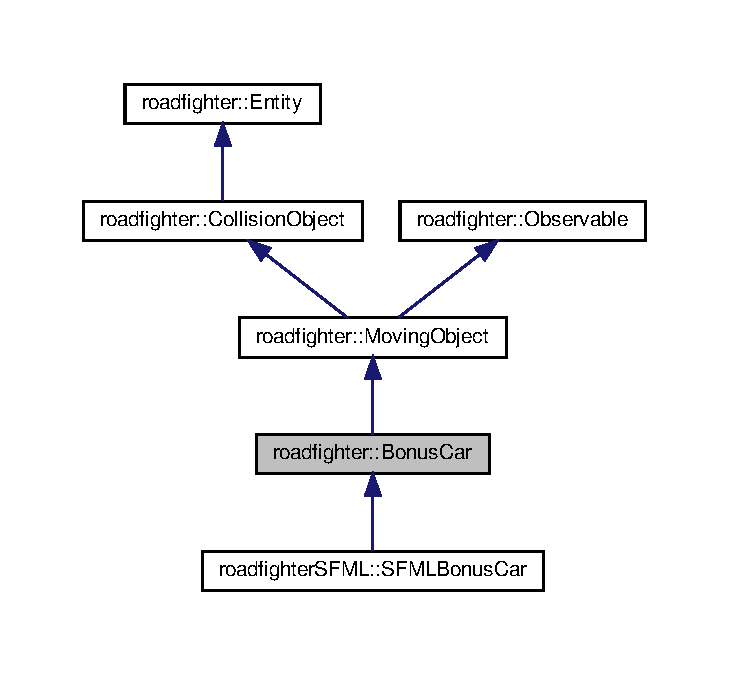
\includegraphics[width=350pt]{classroadfighter_1_1BonusCar__inherit__graph}
\end{center}
\end{figure}


Collaboration diagram for roadfighter\+:\+:Bonus\+Car\+:
\nopagebreak
\begin{figure}[H]
\begin{center}
\leavevmode
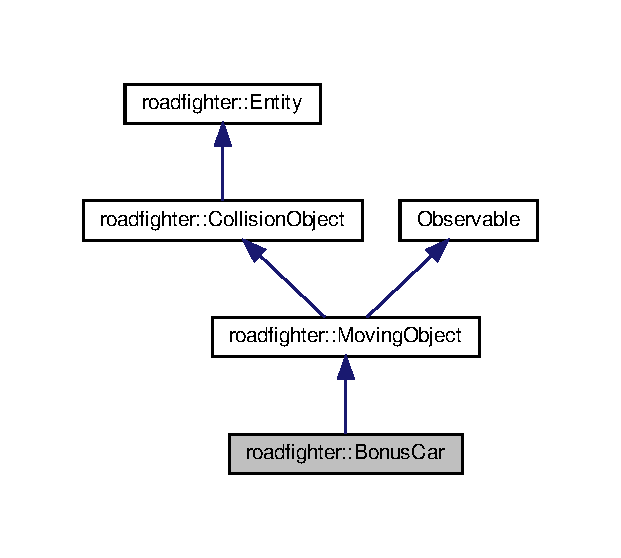
\includegraphics[width=350pt]{classroadfighter_1_1BonusCar__coll__graph}
\end{center}
\end{figure}
\subsection*{Public Member Functions}
\begin{DoxyCompactItemize}
\item 
\hyperlink{classroadfighter_1_1BonusCar_ac759d2c4005dab4bc923cf8e08f50115}{Bonus\+Car} (const \hyperlink{classroadfighter_1_1Location}{Location} \&m\+\_\+loc1, const \hyperlink{classroadfighter_1_1Location}{Location} \&m\+\_\+loc2, double vert\+Speed)
\item 
\hyperlink{classroadfighter_1_1BonusCar_ae0308526b0386e16442bbfdd291f3c29}{Bonus\+Car} (const \hyperlink{classroadfighter_1_1BonusCar}{Bonus\+Car} \&copy)=default
\item 
\hyperlink{classroadfighter_1_1BonusCar_a52b06b6ce44208f2df0e0679193008fa}{Bonus\+Car} (\hyperlink{classroadfighter_1_1BonusCar}{Bonus\+Car} \&\&move)=default
\item 
\hyperlink{classroadfighter_1_1BonusCar}{Bonus\+Car} \& \hyperlink{classroadfighter_1_1BonusCar_acd5303a50571433116089c1f63ab0a9e}{operator=} (const \hyperlink{classroadfighter_1_1BonusCar}{Bonus\+Car} \&other)=default
\item 
\hyperlink{classroadfighter_1_1BonusCar}{Bonus\+Car} \& \hyperlink{classroadfighter_1_1BonusCar_a9fd4f5d8559cd48aa408ff032b92c9f4}{operator=} (\hyperlink{classroadfighter_1_1BonusCar}{Bonus\+Car} \&\&other)=default
\item 
\hyperlink{classroadfighter_1_1BonusCar_a055742bdc09217d56c34c7f582cf7670}{$\sim$\+Bonus\+Car} () override=default
\item 
void \hyperlink{classroadfighter_1_1BonusCar_a21d55ad1e1595ac6c86ca20f8819778b}{update\+Logic} () override
\item 
void \hyperlink{classroadfighter_1_1BonusCar_a2d3d584ca34a5df3b3c833123a9bbc30}{update\+Movement} (double dt) override
\item 
bool \hyperlink{classroadfighter_1_1BonusCar_a19d01e92134634a82ae53f0d017956aa}{must\+Delete} () const override
\item 
void \hyperlink{classroadfighter_1_1BonusCar_ad1ce65b53e5652eac482a7b00c9a1d51}{collide\+With} (std\+::shared\+\_\+ptr$<$ \hyperlink{classroadfighter_1_1CollisionObject}{Collision\+Object} $>$ \&collided) override
\item 
void \hyperlink{classroadfighter_1_1BonusCar_aad0a2a41a1b84c6487c1fc204b5f7cb7}{crash} () override
\item 
void \hyperlink{classroadfighter_1_1BonusCar_a02edcd22a86c1f98642c3703ef8dfb16}{shot} () override
\item 
void \hyperlink{classroadfighter_1_1BonusCar_a3d2d15df036c419cd9ad4fbc6fcd4ad9}{bonus} () override
\item 
void \hyperlink{classroadfighter_1_1BonusCar_afb2d142de799694db896ba875d7d0c27}{win} () override
\end{DoxyCompactItemize}


\subsection{Constructor \& Destructor Documentation}
\mbox{\Hypertarget{classroadfighter_1_1BonusCar_ac759d2c4005dab4bc923cf8e08f50115}\label{classroadfighter_1_1BonusCar_ac759d2c4005dab4bc923cf8e08f50115}} 
\index{roadfighter\+::\+Bonus\+Car@{roadfighter\+::\+Bonus\+Car}!Bonus\+Car@{Bonus\+Car}}
\index{Bonus\+Car@{Bonus\+Car}!roadfighter\+::\+Bonus\+Car@{roadfighter\+::\+Bonus\+Car}}
\subsubsection{\texorpdfstring{Bonus\+Car()}{BonusCar()}\hspace{0.1cm}{\footnotesize\ttfamily [1/3]}}
{\footnotesize\ttfamily roadfighter\+::\+Bonus\+Car\+::\+Bonus\+Car (\begin{DoxyParamCaption}\item[{const \hyperlink{classroadfighter_1_1Location}{Location} \&}]{m\+\_\+loc1,  }\item[{const \hyperlink{classroadfighter_1_1Location}{Location} \&}]{m\+\_\+loc2,  }\item[{double}]{vert\+Speed }\end{DoxyParamCaption})}

constructor where location and speed is given 
\begin{DoxyParams}{Parameters}
{\em m\+\_\+loc1} & first location \\
\hline
{\em m\+\_\+loc2} & second location \\
\hline
{\em vert\+Speed} & \\
\hline
\end{DoxyParams}
\begin{DoxyReturn}{Returns}
none 
\end{DoxyReturn}

\begin{DoxyExceptions}{Exceptions}
{\em none} & \\
\hline
\end{DoxyExceptions}
\mbox{\Hypertarget{classroadfighter_1_1BonusCar_ae0308526b0386e16442bbfdd291f3c29}\label{classroadfighter_1_1BonusCar_ae0308526b0386e16442bbfdd291f3c29}} 
\index{roadfighter\+::\+Bonus\+Car@{roadfighter\+::\+Bonus\+Car}!Bonus\+Car@{Bonus\+Car}}
\index{Bonus\+Car@{Bonus\+Car}!roadfighter\+::\+Bonus\+Car@{roadfighter\+::\+Bonus\+Car}}
\subsubsection{\texorpdfstring{Bonus\+Car()}{BonusCar()}\hspace{0.1cm}{\footnotesize\ttfamily [2/3]}}
{\footnotesize\ttfamily roadfighter\+::\+Bonus\+Car\+::\+Bonus\+Car (\begin{DoxyParamCaption}\item[{const \hyperlink{classroadfighter_1_1BonusCar}{Bonus\+Car} \&}]{copy }\end{DoxyParamCaption})\hspace{0.3cm}{\ttfamily [default]}}

copy constructor 
\begin{DoxyParams}{Parameters}
{\em copy} & the other \hyperlink{classroadfighter_1_1BonusCar}{Bonus\+Car} that is being copied \\
\hline
\end{DoxyParams}
\mbox{\Hypertarget{classroadfighter_1_1BonusCar_a52b06b6ce44208f2df0e0679193008fa}\label{classroadfighter_1_1BonusCar_a52b06b6ce44208f2df0e0679193008fa}} 
\index{roadfighter\+::\+Bonus\+Car@{roadfighter\+::\+Bonus\+Car}!Bonus\+Car@{Bonus\+Car}}
\index{Bonus\+Car@{Bonus\+Car}!roadfighter\+::\+Bonus\+Car@{roadfighter\+::\+Bonus\+Car}}
\subsubsection{\texorpdfstring{Bonus\+Car()}{BonusCar()}\hspace{0.1cm}{\footnotesize\ttfamily [3/3]}}
{\footnotesize\ttfamily roadfighter\+::\+Bonus\+Car\+::\+Bonus\+Car (\begin{DoxyParamCaption}\item[{\hyperlink{classroadfighter_1_1BonusCar}{Bonus\+Car} \&\&}]{move }\end{DoxyParamCaption})\hspace{0.3cm}{\ttfamily [default]}}

move constructor 
\begin{DoxyParams}{Parameters}
{\em Move} & the other \hyperlink{classroadfighter_1_1BonusCar}{Bonus\+Car} that is being moved in this one \\
\hline
\end{DoxyParams}
\mbox{\Hypertarget{classroadfighter_1_1BonusCar_a055742bdc09217d56c34c7f582cf7670}\label{classroadfighter_1_1BonusCar_a055742bdc09217d56c34c7f582cf7670}} 
\index{roadfighter\+::\+Bonus\+Car@{roadfighter\+::\+Bonus\+Car}!````~Bonus\+Car@{$\sim$\+Bonus\+Car}}
\index{````~Bonus\+Car@{$\sim$\+Bonus\+Car}!roadfighter\+::\+Bonus\+Car@{roadfighter\+::\+Bonus\+Car}}
\subsubsection{\texorpdfstring{$\sim$\+Bonus\+Car()}{~BonusCar()}}
{\footnotesize\ttfamily roadfighter\+::\+Bonus\+Car\+::$\sim$\+Bonus\+Car (\begin{DoxyParamCaption}{ }\end{DoxyParamCaption})\hspace{0.3cm}{\ttfamily [override]}, {\ttfamily [default]}}

destructor for \hyperlink{classroadfighter_1_1BonusCar}{Bonus\+Car} 

\subsection{Member Function Documentation}
\mbox{\Hypertarget{classroadfighter_1_1BonusCar_a3d2d15df036c419cd9ad4fbc6fcd4ad9}\label{classroadfighter_1_1BonusCar_a3d2d15df036c419cd9ad4fbc6fcd4ad9}} 
\index{roadfighter\+::\+Bonus\+Car@{roadfighter\+::\+Bonus\+Car}!bonus@{bonus}}
\index{bonus@{bonus}!roadfighter\+::\+Bonus\+Car@{roadfighter\+::\+Bonus\+Car}}
\subsubsection{\texorpdfstring{bonus()}{bonus()}}
{\footnotesize\ttfamily void roadfighter\+::\+Bonus\+Car\+::bonus (\begin{DoxyParamCaption}{ }\end{DoxyParamCaption})\hspace{0.3cm}{\ttfamily [override]}, {\ttfamily [virtual]}}

this function handles the bonus actions of this car \begin{DoxyReturn}{Returns}
none 
\end{DoxyReturn}

\begin{DoxyExceptions}{Exceptions}
{\em none} & \\
\hline
\end{DoxyExceptions}


Reimplemented from \hyperlink{classroadfighter_1_1CollisionObject_ad35887bb3cfb8c054eaaee56306d6944}{roadfighter\+::\+Collision\+Object}.

\mbox{\Hypertarget{classroadfighter_1_1BonusCar_ad1ce65b53e5652eac482a7b00c9a1d51}\label{classroadfighter_1_1BonusCar_ad1ce65b53e5652eac482a7b00c9a1d51}} 
\index{roadfighter\+::\+Bonus\+Car@{roadfighter\+::\+Bonus\+Car}!collide\+With@{collide\+With}}
\index{collide\+With@{collide\+With}!roadfighter\+::\+Bonus\+Car@{roadfighter\+::\+Bonus\+Car}}
\subsubsection{\texorpdfstring{collide\+With()}{collideWith()}}
{\footnotesize\ttfamily void roadfighter\+::\+Bonus\+Car\+::collide\+With (\begin{DoxyParamCaption}\item[{std\+::shared\+\_\+ptr$<$ \hyperlink{classroadfighter_1_1CollisionObject}{Collision\+Object} $>$ \&}]{collided }\end{DoxyParamCaption})\hspace{0.3cm}{\ttfamily [override]}, {\ttfamily [virtual]}}

overidden function from collisionobject that handles what should happen must this car collide with another object for the bonus car it means the the collided function gets the bonus function called on them 
\begin{DoxyParams}{Parameters}
{\em collided} & another object this car collided with \\
\hline
\end{DoxyParams}
\begin{DoxyReturn}{Returns}
none 
\end{DoxyReturn}

\begin{DoxyExceptions}{Exceptions}
{\em none} & \\
\hline
\end{DoxyExceptions}


Reimplemented from \hyperlink{classroadfighter_1_1CollisionObject_a9eba85551432f548f2a0c20217a60f42}{roadfighter\+::\+Collision\+Object}.

\mbox{\Hypertarget{classroadfighter_1_1BonusCar_aad0a2a41a1b84c6487c1fc204b5f7cb7}\label{classroadfighter_1_1BonusCar_aad0a2a41a1b84c6487c1fc204b5f7cb7}} 
\index{roadfighter\+::\+Bonus\+Car@{roadfighter\+::\+Bonus\+Car}!crash@{crash}}
\index{crash@{crash}!roadfighter\+::\+Bonus\+Car@{roadfighter\+::\+Bonus\+Car}}
\subsubsection{\texorpdfstring{crash()}{crash()}}
{\footnotesize\ttfamily void roadfighter\+::\+Bonus\+Car\+::crash (\begin{DoxyParamCaption}{ }\end{DoxyParamCaption})\hspace{0.3cm}{\ttfamily [override]}, {\ttfamily [virtual]}}

this function handles the crashing of the bonuscar \begin{DoxyReturn}{Returns}
none 
\end{DoxyReturn}

\begin{DoxyExceptions}{Exceptions}
{\em none} & \\
\hline
\end{DoxyExceptions}


Reimplemented from \hyperlink{classroadfighter_1_1CollisionObject_a9a5265d810f0ed7583b60046ab3fa88c}{roadfighter\+::\+Collision\+Object}.

\mbox{\Hypertarget{classroadfighter_1_1BonusCar_a19d01e92134634a82ae53f0d017956aa}\label{classroadfighter_1_1BonusCar_a19d01e92134634a82ae53f0d017956aa}} 
\index{roadfighter\+::\+Bonus\+Car@{roadfighter\+::\+Bonus\+Car}!must\+Delete@{must\+Delete}}
\index{must\+Delete@{must\+Delete}!roadfighter\+::\+Bonus\+Car@{roadfighter\+::\+Bonus\+Car}}
\subsubsection{\texorpdfstring{must\+Delete()}{mustDelete()}}
{\footnotesize\ttfamily bool roadfighter\+::\+Bonus\+Car\+::must\+Delete (\begin{DoxyParamCaption}{ }\end{DoxyParamCaption}) const\hspace{0.3cm}{\ttfamily [override]}, {\ttfamily [virtual]}}

a function that will return true if the car should be removed from the game \begin{DoxyReturn}{Returns}
a bool 
\end{DoxyReturn}

\begin{DoxyExceptions}{Exceptions}
{\em none} & \\
\hline
\end{DoxyExceptions}


Reimplemented from \hyperlink{classroadfighter_1_1CollisionObject_a738071cd7b1b8cd4c8d455b5e552bd4c}{roadfighter\+::\+Collision\+Object}.

\mbox{\Hypertarget{classroadfighter_1_1BonusCar_acd5303a50571433116089c1f63ab0a9e}\label{classroadfighter_1_1BonusCar_acd5303a50571433116089c1f63ab0a9e}} 
\index{roadfighter\+::\+Bonus\+Car@{roadfighter\+::\+Bonus\+Car}!operator=@{operator=}}
\index{operator=@{operator=}!roadfighter\+::\+Bonus\+Car@{roadfighter\+::\+Bonus\+Car}}
\subsubsection{\texorpdfstring{operator=()}{operator=()}\hspace{0.1cm}{\footnotesize\ttfamily [1/2]}}
{\footnotesize\ttfamily \hyperlink{classroadfighter_1_1BonusCar}{Bonus\+Car}\& roadfighter\+::\+Bonus\+Car\+::operator= (\begin{DoxyParamCaption}\item[{const \hyperlink{classroadfighter_1_1BonusCar}{Bonus\+Car} \&}]{other }\end{DoxyParamCaption})\hspace{0.3cm}{\ttfamily [default]}}

copy assignment for \hyperlink{classroadfighter_1_1BonusCar}{Bonus\+Car} 
\begin{DoxyParams}{Parameters}
{\em other} & the \hyperlink{classroadfighter_1_1BonusCar}{Bonus\+Car} that is being copied \\
\hline
\end{DoxyParams}
\begin{DoxyReturn}{Returns}
a new \hyperlink{classroadfighter_1_1BonusCar}{Bonus\+Car} that is equal to the other one 
\end{DoxyReturn}
\mbox{\Hypertarget{classroadfighter_1_1BonusCar_a9fd4f5d8559cd48aa408ff032b92c9f4}\label{classroadfighter_1_1BonusCar_a9fd4f5d8559cd48aa408ff032b92c9f4}} 
\index{roadfighter\+::\+Bonus\+Car@{roadfighter\+::\+Bonus\+Car}!operator=@{operator=}}
\index{operator=@{operator=}!roadfighter\+::\+Bonus\+Car@{roadfighter\+::\+Bonus\+Car}}
\subsubsection{\texorpdfstring{operator=()}{operator=()}\hspace{0.1cm}{\footnotesize\ttfamily [2/2]}}
{\footnotesize\ttfamily \hyperlink{classroadfighter_1_1BonusCar}{Bonus\+Car}\& roadfighter\+::\+Bonus\+Car\+::operator= (\begin{DoxyParamCaption}\item[{\hyperlink{classroadfighter_1_1BonusCar}{Bonus\+Car} \&\&}]{other }\end{DoxyParamCaption})\hspace{0.3cm}{\ttfamily [default]}}

move assignment for \hyperlink{classroadfighter_1_1BonusCar}{Bonus\+Car} 
\begin{DoxyParams}{Parameters}
{\em other} & other \hyperlink{classroadfighter_1_1BonusCar}{Bonus\+Car} that is being moved \\
\hline
\end{DoxyParams}
\begin{DoxyReturn}{Returns}
a \hyperlink{classroadfighter_1_1BonusCar}{Bonus\+Car} that contains all the data of the first one 
\end{DoxyReturn}
\mbox{\Hypertarget{classroadfighter_1_1BonusCar_a02edcd22a86c1f98642c3703ef8dfb16}\label{classroadfighter_1_1BonusCar_a02edcd22a86c1f98642c3703ef8dfb16}} 
\index{roadfighter\+::\+Bonus\+Car@{roadfighter\+::\+Bonus\+Car}!shot@{shot}}
\index{shot@{shot}!roadfighter\+::\+Bonus\+Car@{roadfighter\+::\+Bonus\+Car}}
\subsubsection{\texorpdfstring{shot()}{shot()}}
{\footnotesize\ttfamily void roadfighter\+::\+Bonus\+Car\+::shot (\begin{DoxyParamCaption}{ }\end{DoxyParamCaption})\hspace{0.3cm}{\ttfamily [override]}, {\ttfamily [virtual]}}

this function handles the being shot of the bonuscar \begin{DoxyReturn}{Returns}
none 
\end{DoxyReturn}

\begin{DoxyExceptions}{Exceptions}
{\em none} & \\
\hline
\end{DoxyExceptions}


Reimplemented from \hyperlink{classroadfighter_1_1CollisionObject_a55d891b6d9b50abdc44f964a40a7777c}{roadfighter\+::\+Collision\+Object}.

\mbox{\Hypertarget{classroadfighter_1_1BonusCar_a21d55ad1e1595ac6c86ca20f8819778b}\label{classroadfighter_1_1BonusCar_a21d55ad1e1595ac6c86ca20f8819778b}} 
\index{roadfighter\+::\+Bonus\+Car@{roadfighter\+::\+Bonus\+Car}!update\+Logic@{update\+Logic}}
\index{update\+Logic@{update\+Logic}!roadfighter\+::\+Bonus\+Car@{roadfighter\+::\+Bonus\+Car}}
\subsubsection{\texorpdfstring{update\+Logic()}{updateLogic()}}
{\footnotesize\ttfamily void roadfighter\+::\+Bonus\+Car\+::update\+Logic (\begin{DoxyParamCaption}{ }\end{DoxyParamCaption})\hspace{0.3cm}{\ttfamily [override]}, {\ttfamily [virtual]}}

updates the logic of the bonus car \begin{DoxyReturn}{Returns}
none 
\end{DoxyReturn}

\begin{DoxyExceptions}{Exceptions}
{\em none} & \\
\hline
\end{DoxyExceptions}


Implements \hyperlink{classroadfighter_1_1Entity_a54c00f1af306290bae3e4b84e196566b}{roadfighter\+::\+Entity}.

\mbox{\Hypertarget{classroadfighter_1_1BonusCar_a2d3d584ca34a5df3b3c833123a9bbc30}\label{classroadfighter_1_1BonusCar_a2d3d584ca34a5df3b3c833123a9bbc30}} 
\index{roadfighter\+::\+Bonus\+Car@{roadfighter\+::\+Bonus\+Car}!update\+Movement@{update\+Movement}}
\index{update\+Movement@{update\+Movement}!roadfighter\+::\+Bonus\+Car@{roadfighter\+::\+Bonus\+Car}}
\subsubsection{\texorpdfstring{update\+Movement()}{updateMovement()}}
{\footnotesize\ttfamily void roadfighter\+::\+Bonus\+Car\+::update\+Movement (\begin{DoxyParamCaption}\item[{double}]{dt }\end{DoxyParamCaption})\hspace{0.3cm}{\ttfamily [override]}, {\ttfamily [virtual]}}

updates the movement of the bonus car with dt ticks 
\begin{DoxyParams}{Parameters}
{\em dt} & the amount of a tick the car should move forward \\
\hline
\end{DoxyParams}
\begin{DoxyReturn}{Returns}
none 
\end{DoxyReturn}

\begin{DoxyExceptions}{Exceptions}
{\em none} & \\
\hline
\end{DoxyExceptions}


Implements \hyperlink{classroadfighter_1_1Entity_a66614a11004d6f9516473f60b530f689}{roadfighter\+::\+Entity}.

\mbox{\Hypertarget{classroadfighter_1_1BonusCar_afb2d142de799694db896ba875d7d0c27}\label{classroadfighter_1_1BonusCar_afb2d142de799694db896ba875d7d0c27}} 
\index{roadfighter\+::\+Bonus\+Car@{roadfighter\+::\+Bonus\+Car}!win@{win}}
\index{win@{win}!roadfighter\+::\+Bonus\+Car@{roadfighter\+::\+Bonus\+Car}}
\subsubsection{\texorpdfstring{win()}{win()}}
{\footnotesize\ttfamily void roadfighter\+::\+Bonus\+Car\+::win (\begin{DoxyParamCaption}{ }\end{DoxyParamCaption})\hspace{0.3cm}{\ttfamily [override]}, {\ttfamily [virtual]}}

this function handles the win condition for this car \begin{DoxyReturn}{Returns}
none 
\end{DoxyReturn}

\begin{DoxyExceptions}{Exceptions}
{\em none} & \\
\hline
\end{DoxyExceptions}


Reimplemented from \hyperlink{classroadfighter_1_1CollisionObject_aa793e1b9943ee90bbb4129ddd06b9be7}{roadfighter\+::\+Collision\+Object}.



The documentation for this class was generated from the following files\+:\begin{DoxyCompactItemize}
\item 
Game\+Logic/include/\+Entities/\hyperlink{BonusCar_8h}{Bonus\+Car.\+h}\item 
Game\+Logic/\+Source/\+Entities/\hyperlink{BonusCar_8cpp}{Bonus\+Car.\+cpp}\end{DoxyCompactItemize}

\hypertarget{classroadfighter_1_1Bullet}{}\section{roadfighter\+:\+:Bullet Class Reference}
\label{classroadfighter_1_1Bullet}\index{roadfighter\+::\+Bullet@{roadfighter\+::\+Bullet}}


Inheritance diagram for roadfighter\+:\+:Bullet\+:
\nopagebreak
\begin{figure}[H]
\begin{center}
\leavevmode
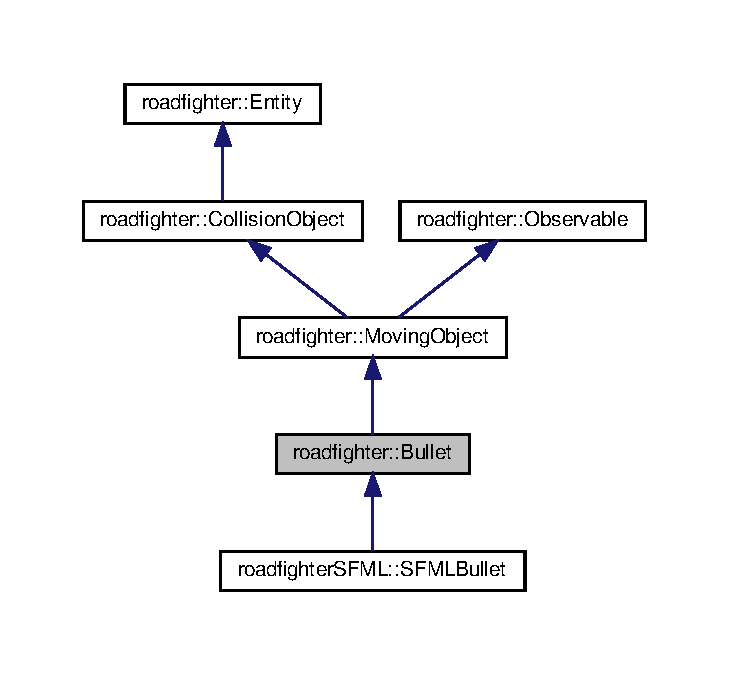
\includegraphics[width=350pt]{classroadfighter_1_1Bullet__inherit__graph}
\end{center}
\end{figure}


Collaboration diagram for roadfighter\+:\+:Bullet\+:
\nopagebreak
\begin{figure}[H]
\begin{center}
\leavevmode
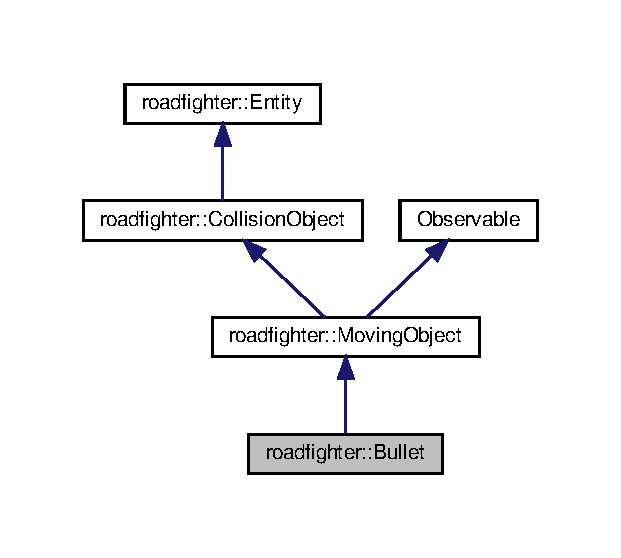
\includegraphics[width=350pt]{classroadfighter_1_1Bullet__coll__graph}
\end{center}
\end{figure}
\subsection*{Public Member Functions}
\begin{DoxyCompactItemize}
\item 
\hyperlink{classroadfighter_1_1Bullet_abae3f231af0b423fc6ca0d0d5639fed5}{Bullet} ()=default
\item 
\hyperlink{classroadfighter_1_1Bullet_a5ee7b1e8b458efef1c60ed1acebb8e9e}{Bullet} (const \hyperlink{classroadfighter_1_1Bullet}{Bullet} \&copy)=default
\item 
\hyperlink{classroadfighter_1_1Bullet_a20d663e607a956782dcaee5fc514da5c}{Bullet} (\hyperlink{classroadfighter_1_1Bullet}{Bullet} \&\&move)=default
\item 
\hyperlink{classroadfighter_1_1Bullet_a15ab9848b269b1ef463defbb6967deb0}{Bullet} (const \hyperlink{classroadfighter_1_1Location}{Location} \&m\+\_\+loc1, const \hyperlink{classroadfighter_1_1Location}{Location} \&m\+\_\+loc2, double vertspeed)
\item 
\hyperlink{classroadfighter_1_1Bullet}{Bullet} \& \hyperlink{classroadfighter_1_1Bullet_ab507000db2f726b8906ced3ea4c7782f}{operator=} (const \hyperlink{classroadfighter_1_1Bullet}{Bullet} \&other)=default
\item 
\hyperlink{classroadfighter_1_1Bullet}{Bullet} \& \hyperlink{classroadfighter_1_1Bullet_a7c63a2a326738605af30ad850272d3b7}{operator=} (\hyperlink{classroadfighter_1_1Bullet}{Bullet} \&\&other)=default
\item 
\hyperlink{classroadfighter_1_1Bullet_a297de09c51315af09bd676801cc4e2bd}{$\sim$\+Bullet} () override=default
\item 
void \hyperlink{classroadfighter_1_1Bullet_a36156632331e59c11abf5ae76024bc1f}{collide\+With} (std\+::shared\+\_\+ptr$<$ \hyperlink{classroadfighter_1_1CollisionObject}{Collision\+Object} $>$ \&collided) override
\item 
void \hyperlink{classroadfighter_1_1Bullet_ac96121377fffa9ed8ea94c333a841a7a}{crash} () override
\item 
void \hyperlink{classroadfighter_1_1Bullet_acaacd303f1f4e55c5029d4a4cbe1d9b1}{shot} () override
\item 
void \hyperlink{classroadfighter_1_1Bullet_a642ca8467a0ffea844d18d4917b2f49e}{bonus} () override
\item 
void \hyperlink{classroadfighter_1_1Bullet_a566adb0235665312365cd65536c2aafc}{win} () override
\item 
void \hyperlink{classroadfighter_1_1Bullet_a13aa730279ee8590d0eb2f9e6c01f265}{update\+Logic} () override
\item 
bool \hyperlink{classroadfighter_1_1Bullet_a0f87b693a1583522e551ba1324fcd067}{must\+Delete} () const override
\end{DoxyCompactItemize}


\subsection{Constructor \& Destructor Documentation}
\mbox{\Hypertarget{classroadfighter_1_1Bullet_abae3f231af0b423fc6ca0d0d5639fed5}\label{classroadfighter_1_1Bullet_abae3f231af0b423fc6ca0d0d5639fed5}} 
\index{roadfighter\+::\+Bullet@{roadfighter\+::\+Bullet}!Bullet@{Bullet}}
\index{Bullet@{Bullet}!roadfighter\+::\+Bullet@{roadfighter\+::\+Bullet}}
\subsubsection{\texorpdfstring{Bullet()}{Bullet()}\hspace{0.1cm}{\footnotesize\ttfamily [1/4]}}
{\footnotesize\ttfamily roadfighter\+::\+Bullet\+::\+Bullet (\begin{DoxyParamCaption}{ }\end{DoxyParamCaption})\hspace{0.3cm}{\ttfamily [default]}}

default constructor for \hyperlink{classroadfighter_1_1Bullet}{Bullet} \mbox{\Hypertarget{classroadfighter_1_1Bullet_a5ee7b1e8b458efef1c60ed1acebb8e9e}\label{classroadfighter_1_1Bullet_a5ee7b1e8b458efef1c60ed1acebb8e9e}} 
\index{roadfighter\+::\+Bullet@{roadfighter\+::\+Bullet}!Bullet@{Bullet}}
\index{Bullet@{Bullet}!roadfighter\+::\+Bullet@{roadfighter\+::\+Bullet}}
\subsubsection{\texorpdfstring{Bullet()}{Bullet()}\hspace{0.1cm}{\footnotesize\ttfamily [2/4]}}
{\footnotesize\ttfamily roadfighter\+::\+Bullet\+::\+Bullet (\begin{DoxyParamCaption}\item[{const \hyperlink{classroadfighter_1_1Bullet}{Bullet} \&}]{copy }\end{DoxyParamCaption})\hspace{0.3cm}{\ttfamily [default]}}

copy constructor 
\begin{DoxyParams}{Parameters}
{\em copy} & the other \hyperlink{classroadfighter_1_1Bullet}{Bullet} that is being copied \\
\hline
\end{DoxyParams}
\mbox{\Hypertarget{classroadfighter_1_1Bullet_a20d663e607a956782dcaee5fc514da5c}\label{classroadfighter_1_1Bullet_a20d663e607a956782dcaee5fc514da5c}} 
\index{roadfighter\+::\+Bullet@{roadfighter\+::\+Bullet}!Bullet@{Bullet}}
\index{Bullet@{Bullet}!roadfighter\+::\+Bullet@{roadfighter\+::\+Bullet}}
\subsubsection{\texorpdfstring{Bullet()}{Bullet()}\hspace{0.1cm}{\footnotesize\ttfamily [3/4]}}
{\footnotesize\ttfamily roadfighter\+::\+Bullet\+::\+Bullet (\begin{DoxyParamCaption}\item[{\hyperlink{classroadfighter_1_1Bullet}{Bullet} \&\&}]{move }\end{DoxyParamCaption})\hspace{0.3cm}{\ttfamily [default]}}

move constructor 
\begin{DoxyParams}{Parameters}
{\em Move} & the other \hyperlink{classroadfighter_1_1Bullet}{Bullet} that is being moved in this one \\
\hline
\end{DoxyParams}
\mbox{\Hypertarget{classroadfighter_1_1Bullet_a15ab9848b269b1ef463defbb6967deb0}\label{classroadfighter_1_1Bullet_a15ab9848b269b1ef463defbb6967deb0}} 
\index{roadfighter\+::\+Bullet@{roadfighter\+::\+Bullet}!Bullet@{Bullet}}
\index{Bullet@{Bullet}!roadfighter\+::\+Bullet@{roadfighter\+::\+Bullet}}
\subsubsection{\texorpdfstring{Bullet()}{Bullet()}\hspace{0.1cm}{\footnotesize\ttfamily [4/4]}}
{\footnotesize\ttfamily roadfighter\+::\+Bullet\+::\+Bullet (\begin{DoxyParamCaption}\item[{const \hyperlink{classroadfighter_1_1Location}{Location} \&}]{m\+\_\+loc1,  }\item[{const \hyperlink{classroadfighter_1_1Location}{Location} \&}]{m\+\_\+loc2,  }\item[{double}]{vertspeed }\end{DoxyParamCaption})}

constructor by values 
\begin{DoxyParams}{Parameters}
{\em m\+\_\+loc1} & first gamelocation(upper left corner) \\
\hline
{\em m\+\_\+loc2} & second gamelocation (upper right corner) \\
\hline
{\em m\+\_\+max\+Vert\+Speed} & \\
\hline
{\em m\+\_\+vert\+Accel} & \\
\hline
{\em m\+\_\+hor\+Accel} & constructor where all variables are given \\
\hline
{\em m\+\_\+loc1} & first location \\
\hline
{\em m\+\_\+loc2} & second location \\
\hline
{\em vertspeed} & vertical speed \\
\hline
\end{DoxyParams}
\begin{DoxyReturn}{Returns}
none  none 
\end{DoxyReturn}
\mbox{\Hypertarget{classroadfighter_1_1Bullet_a297de09c51315af09bd676801cc4e2bd}\label{classroadfighter_1_1Bullet_a297de09c51315af09bd676801cc4e2bd}} 
\index{roadfighter\+::\+Bullet@{roadfighter\+::\+Bullet}!````~Bullet@{$\sim$\+Bullet}}
\index{````~Bullet@{$\sim$\+Bullet}!roadfighter\+::\+Bullet@{roadfighter\+::\+Bullet}}
\subsubsection{\texorpdfstring{$\sim$\+Bullet()}{~Bullet()}}
{\footnotesize\ttfamily roadfighter\+::\+Bullet\+::$\sim$\+Bullet (\begin{DoxyParamCaption}{ }\end{DoxyParamCaption})\hspace{0.3cm}{\ttfamily [override]}, {\ttfamily [default]}}

destructor for \hyperlink{classroadfighter_1_1Bullet}{Bullet} 

\subsection{Member Function Documentation}
\mbox{\Hypertarget{classroadfighter_1_1Bullet_a642ca8467a0ffea844d18d4917b2f49e}\label{classroadfighter_1_1Bullet_a642ca8467a0ffea844d18d4917b2f49e}} 
\index{roadfighter\+::\+Bullet@{roadfighter\+::\+Bullet}!bonus@{bonus}}
\index{bonus@{bonus}!roadfighter\+::\+Bullet@{roadfighter\+::\+Bullet}}
\subsubsection{\texorpdfstring{bonus()}{bonus()}}
{\footnotesize\ttfamily void roadfighter\+::\+Bullet\+::bonus (\begin{DoxyParamCaption}{ }\end{DoxyParamCaption})\hspace{0.3cm}{\ttfamily [override]}, {\ttfamily [virtual]}}

this function handles the bonus function of the bullet \begin{DoxyReturn}{Returns}
none 
\end{DoxyReturn}

\begin{DoxyExceptions}{Exceptions}
{\em none} & \\
\hline
\end{DoxyExceptions}


Reimplemented from \hyperlink{classroadfighter_1_1CollisionObject_ad35887bb3cfb8c054eaaee56306d6944}{roadfighter\+::\+Collision\+Object}.

\mbox{\Hypertarget{classroadfighter_1_1Bullet_a36156632331e59c11abf5ae76024bc1f}\label{classroadfighter_1_1Bullet_a36156632331e59c11abf5ae76024bc1f}} 
\index{roadfighter\+::\+Bullet@{roadfighter\+::\+Bullet}!collide\+With@{collide\+With}}
\index{collide\+With@{collide\+With}!roadfighter\+::\+Bullet@{roadfighter\+::\+Bullet}}
\subsubsection{\texorpdfstring{collide\+With()}{collideWith()}}
{\footnotesize\ttfamily void roadfighter\+::\+Bullet\+::collide\+With (\begin{DoxyParamCaption}\item[{std\+::shared\+\_\+ptr$<$ \hyperlink{classroadfighter_1_1CollisionObject}{Collision\+Object} $>$ \&}]{collided }\end{DoxyParamCaption})\hspace{0.3cm}{\ttfamily [override]}, {\ttfamily [virtual]}}

this function handles what should happen must a object colldie with this bullet here it means the object get shot 
\begin{DoxyParams}{Parameters}
{\em collided} & the object the bullet collides with \\
\hline
\end{DoxyParams}
\begin{DoxyReturn}{Returns}
none 
\end{DoxyReturn}

\begin{DoxyExceptions}{Exceptions}
{\em none} & \\
\hline
\end{DoxyExceptions}


Reimplemented from \hyperlink{classroadfighter_1_1CollisionObject_a9eba85551432f548f2a0c20217a60f42}{roadfighter\+::\+Collision\+Object}.

\mbox{\Hypertarget{classroadfighter_1_1Bullet_ac96121377fffa9ed8ea94c333a841a7a}\label{classroadfighter_1_1Bullet_ac96121377fffa9ed8ea94c333a841a7a}} 
\index{roadfighter\+::\+Bullet@{roadfighter\+::\+Bullet}!crash@{crash}}
\index{crash@{crash}!roadfighter\+::\+Bullet@{roadfighter\+::\+Bullet}}
\subsubsection{\texorpdfstring{crash()}{crash()}}
{\footnotesize\ttfamily void roadfighter\+::\+Bullet\+::crash (\begin{DoxyParamCaption}{ }\end{DoxyParamCaption})\hspace{0.3cm}{\ttfamily [override]}, {\ttfamily [virtual]}}

this function handles the crash of a bullet \begin{DoxyReturn}{Returns}
none 
\end{DoxyReturn}

\begin{DoxyExceptions}{Exceptions}
{\em none} & \\
\hline
\end{DoxyExceptions}


Reimplemented from \hyperlink{classroadfighter_1_1CollisionObject_a9a5265d810f0ed7583b60046ab3fa88c}{roadfighter\+::\+Collision\+Object}.

\mbox{\Hypertarget{classroadfighter_1_1Bullet_a0f87b693a1583522e551ba1324fcd067}\label{classroadfighter_1_1Bullet_a0f87b693a1583522e551ba1324fcd067}} 
\index{roadfighter\+::\+Bullet@{roadfighter\+::\+Bullet}!must\+Delete@{must\+Delete}}
\index{must\+Delete@{must\+Delete}!roadfighter\+::\+Bullet@{roadfighter\+::\+Bullet}}
\subsubsection{\texorpdfstring{must\+Delete()}{mustDelete()}}
{\footnotesize\ttfamily bool roadfighter\+::\+Bullet\+::must\+Delete (\begin{DoxyParamCaption}{ }\end{DoxyParamCaption}) const\hspace{0.3cm}{\ttfamily [override]}, {\ttfamily [virtual]}}

overidden function that denotes whether the bullet must be deleted or not \begin{DoxyReturn}{Returns}
a bool 
\end{DoxyReturn}

\begin{DoxyExceptions}{Exceptions}
{\em none} & \\
\hline
\end{DoxyExceptions}


Reimplemented from \hyperlink{classroadfighter_1_1CollisionObject_a738071cd7b1b8cd4c8d455b5e552bd4c}{roadfighter\+::\+Collision\+Object}.

\mbox{\Hypertarget{classroadfighter_1_1Bullet_ab507000db2f726b8906ced3ea4c7782f}\label{classroadfighter_1_1Bullet_ab507000db2f726b8906ced3ea4c7782f}} 
\index{roadfighter\+::\+Bullet@{roadfighter\+::\+Bullet}!operator=@{operator=}}
\index{operator=@{operator=}!roadfighter\+::\+Bullet@{roadfighter\+::\+Bullet}}
\subsubsection{\texorpdfstring{operator=()}{operator=()}\hspace{0.1cm}{\footnotesize\ttfamily [1/2]}}
{\footnotesize\ttfamily \hyperlink{classroadfighter_1_1Bullet}{Bullet}\& roadfighter\+::\+Bullet\+::operator= (\begin{DoxyParamCaption}\item[{const \hyperlink{classroadfighter_1_1Bullet}{Bullet} \&}]{other }\end{DoxyParamCaption})\hspace{0.3cm}{\ttfamily [default]}}

copy assigment for \hyperlink{classroadfighter_1_1Bullet}{Bullet} 
\begin{DoxyParams}{Parameters}
{\em other} & the \hyperlink{classroadfighter_1_1Bullet}{Bullet} that is being copied \\
\hline
\end{DoxyParams}
\begin{DoxyReturn}{Returns}
a new \hyperlink{classroadfighter_1_1Bullet}{Bullet} that is equal to the other one 
\end{DoxyReturn}
\mbox{\Hypertarget{classroadfighter_1_1Bullet_a7c63a2a326738605af30ad850272d3b7}\label{classroadfighter_1_1Bullet_a7c63a2a326738605af30ad850272d3b7}} 
\index{roadfighter\+::\+Bullet@{roadfighter\+::\+Bullet}!operator=@{operator=}}
\index{operator=@{operator=}!roadfighter\+::\+Bullet@{roadfighter\+::\+Bullet}}
\subsubsection{\texorpdfstring{operator=()}{operator=()}\hspace{0.1cm}{\footnotesize\ttfamily [2/2]}}
{\footnotesize\ttfamily \hyperlink{classroadfighter_1_1Bullet}{Bullet}\& roadfighter\+::\+Bullet\+::operator= (\begin{DoxyParamCaption}\item[{\hyperlink{classroadfighter_1_1Bullet}{Bullet} \&\&}]{other }\end{DoxyParamCaption})\hspace{0.3cm}{\ttfamily [default]}}

move assignment for \hyperlink{classroadfighter_1_1Bullet}{Bullet} 
\begin{DoxyParams}{Parameters}
{\em other} & other \hyperlink{classroadfighter_1_1Bullet}{Bullet} that is being moved \\
\hline
\end{DoxyParams}
\begin{DoxyReturn}{Returns}
a \hyperlink{classroadfighter_1_1Bullet}{Bullet} that contains all the data of the first one 
\end{DoxyReturn}
\mbox{\Hypertarget{classroadfighter_1_1Bullet_acaacd303f1f4e55c5029d4a4cbe1d9b1}\label{classroadfighter_1_1Bullet_acaacd303f1f4e55c5029d4a4cbe1d9b1}} 
\index{roadfighter\+::\+Bullet@{roadfighter\+::\+Bullet}!shot@{shot}}
\index{shot@{shot}!roadfighter\+::\+Bullet@{roadfighter\+::\+Bullet}}
\subsubsection{\texorpdfstring{shot()}{shot()}}
{\footnotesize\ttfamily void roadfighter\+::\+Bullet\+::shot (\begin{DoxyParamCaption}{ }\end{DoxyParamCaption})\hspace{0.3cm}{\ttfamily [override]}, {\ttfamily [virtual]}}

this function handles the shot logic of the bullet \begin{DoxyReturn}{Returns}
none 
\end{DoxyReturn}

\begin{DoxyExceptions}{Exceptions}
{\em none} & \\
\hline
\end{DoxyExceptions}


Reimplemented from \hyperlink{classroadfighter_1_1CollisionObject_a55d891b6d9b50abdc44f964a40a7777c}{roadfighter\+::\+Collision\+Object}.

\mbox{\Hypertarget{classroadfighter_1_1Bullet_a13aa730279ee8590d0eb2f9e6c01f265}\label{classroadfighter_1_1Bullet_a13aa730279ee8590d0eb2f9e6c01f265}} 
\index{roadfighter\+::\+Bullet@{roadfighter\+::\+Bullet}!update\+Logic@{update\+Logic}}
\index{update\+Logic@{update\+Logic}!roadfighter\+::\+Bullet@{roadfighter\+::\+Bullet}}
\subsubsection{\texorpdfstring{update\+Logic()}{updateLogic()}}
{\footnotesize\ttfamily void roadfighter\+::\+Bullet\+::update\+Logic (\begin{DoxyParamCaption}{ }\end{DoxyParamCaption})\hspace{0.3cm}{\ttfamily [override]}, {\ttfamily [virtual]}}

overidden function that updates the logic of the bullet \begin{DoxyReturn}{Returns}
none 
\end{DoxyReturn}

\begin{DoxyExceptions}{Exceptions}
{\em none} & \\
\hline
\end{DoxyExceptions}


Implements \hyperlink{classroadfighter_1_1Entity_a54c00f1af306290bae3e4b84e196566b}{roadfighter\+::\+Entity}.

\mbox{\Hypertarget{classroadfighter_1_1Bullet_a566adb0235665312365cd65536c2aafc}\label{classroadfighter_1_1Bullet_a566adb0235665312365cd65536c2aafc}} 
\index{roadfighter\+::\+Bullet@{roadfighter\+::\+Bullet}!win@{win}}
\index{win@{win}!roadfighter\+::\+Bullet@{roadfighter\+::\+Bullet}}
\subsubsection{\texorpdfstring{win()}{win()}}
{\footnotesize\ttfamily void roadfighter\+::\+Bullet\+::win (\begin{DoxyParamCaption}{ }\end{DoxyParamCaption})\hspace{0.3cm}{\ttfamily [override]}, {\ttfamily [virtual]}}

this function handles the win condition of a bullet \begin{DoxyReturn}{Returns}
none 
\end{DoxyReturn}

\begin{DoxyExceptions}{Exceptions}
{\em } & \\
\hline
\end{DoxyExceptions}


Reimplemented from \hyperlink{classroadfighter_1_1CollisionObject_aa793e1b9943ee90bbb4129ddd06b9be7}{roadfighter\+::\+Collision\+Object}.



The documentation for this class was generated from the following files\+:\begin{DoxyCompactItemize}
\item 
Game\+Logic/include/\+Entities/\hyperlink{Bullet_8h}{Bullet.\+h}\item 
Game\+Logic/\+Source/\+Entities/\hyperlink{Bullet_8cpp}{Bullet.\+cpp}\end{DoxyCompactItemize}

\hypertarget{classClock}{}\section{Clock Class Reference}
\label{classClock}\index{Clock@{Clock}}


{\ttfamily \#include $<$Clock.\+h$>$}

\subsection*{Public Member Functions}
\begin{DoxyCompactItemize}
\item 
\hyperlink{classClock_adbc370eb6b5f8d01645cf440188160a8}{Clock} ()
\item 
void \hyperlink{classClock_a775bf97123b58c768571868341d28b08}{restart} ()
\item 
double \hyperlink{classClock_af7e4352c60e4268d43a0489dfb541c9f}{get\+Time\+As\+Seconds} ()
\end{DoxyCompactItemize}


\subsection{Detailed Description}
an encapsulation for the c++ clock library to make it easier to use 

\subsection{Constructor \& Destructor Documentation}
\mbox{\Hypertarget{classClock_adbc370eb6b5f8d01645cf440188160a8}\label{classClock_adbc370eb6b5f8d01645cf440188160a8}} 
\index{Clock@{Clock}!Clock@{Clock}}
\index{Clock@{Clock}!Clock@{Clock}}
\subsubsection{\texorpdfstring{Clock()}{Clock()}}
{\footnotesize\ttfamily Clock\+::\+Clock (\begin{DoxyParamCaption}{ }\end{DoxyParamCaption})}

default and only constructor, the time starts teh second this clock is created 

\subsection{Member Function Documentation}
\mbox{\Hypertarget{classClock_af7e4352c60e4268d43a0489dfb541c9f}\label{classClock_af7e4352c60e4268d43a0489dfb541c9f}} 
\index{Clock@{Clock}!get\+Time\+As\+Seconds@{get\+Time\+As\+Seconds}}
\index{get\+Time\+As\+Seconds@{get\+Time\+As\+Seconds}!Clock@{Clock}}
\subsubsection{\texorpdfstring{get\+Time\+As\+Seconds()}{getTimeAsSeconds()}}
{\footnotesize\ttfamily double Clock\+::get\+Time\+As\+Seconds (\begin{DoxyParamCaption}{ }\end{DoxyParamCaption})}

gets the amount of time that has passed since construction or last reset \begin{DoxyReturn}{Returns}
this time as seconds in a double 
\end{DoxyReturn}
\mbox{\Hypertarget{classClock_a775bf97123b58c768571868341d28b08}\label{classClock_a775bf97123b58c768571868341d28b08}} 
\index{Clock@{Clock}!restart@{restart}}
\index{restart@{restart}!Clock@{Clock}}
\subsubsection{\texorpdfstring{restart()}{restart()}}
{\footnotesize\ttfamily void Clock\+::restart (\begin{DoxyParamCaption}{ }\end{DoxyParamCaption})}

restart the clock 

The documentation for this class was generated from the following files\+:\begin{DoxyCompactItemize}
\item 
Game\+Logic/\+Utility/Clock.\+h\item 
Game\+Logic/\+Utility/Clock.\+cpp\end{DoxyCompactItemize}

\hypertarget{classroadfighter_1_1CollisionObject}{}\section{roadfighter\+:\+:Collision\+Object Class Reference}
\label{classroadfighter_1_1CollisionObject}\index{roadfighter\+::\+Collision\+Object@{roadfighter\+::\+Collision\+Object}}


Inheritance diagram for roadfighter\+:\+:Collision\+Object\+:
\nopagebreak
\begin{figure}[H]
\begin{center}
\leavevmode
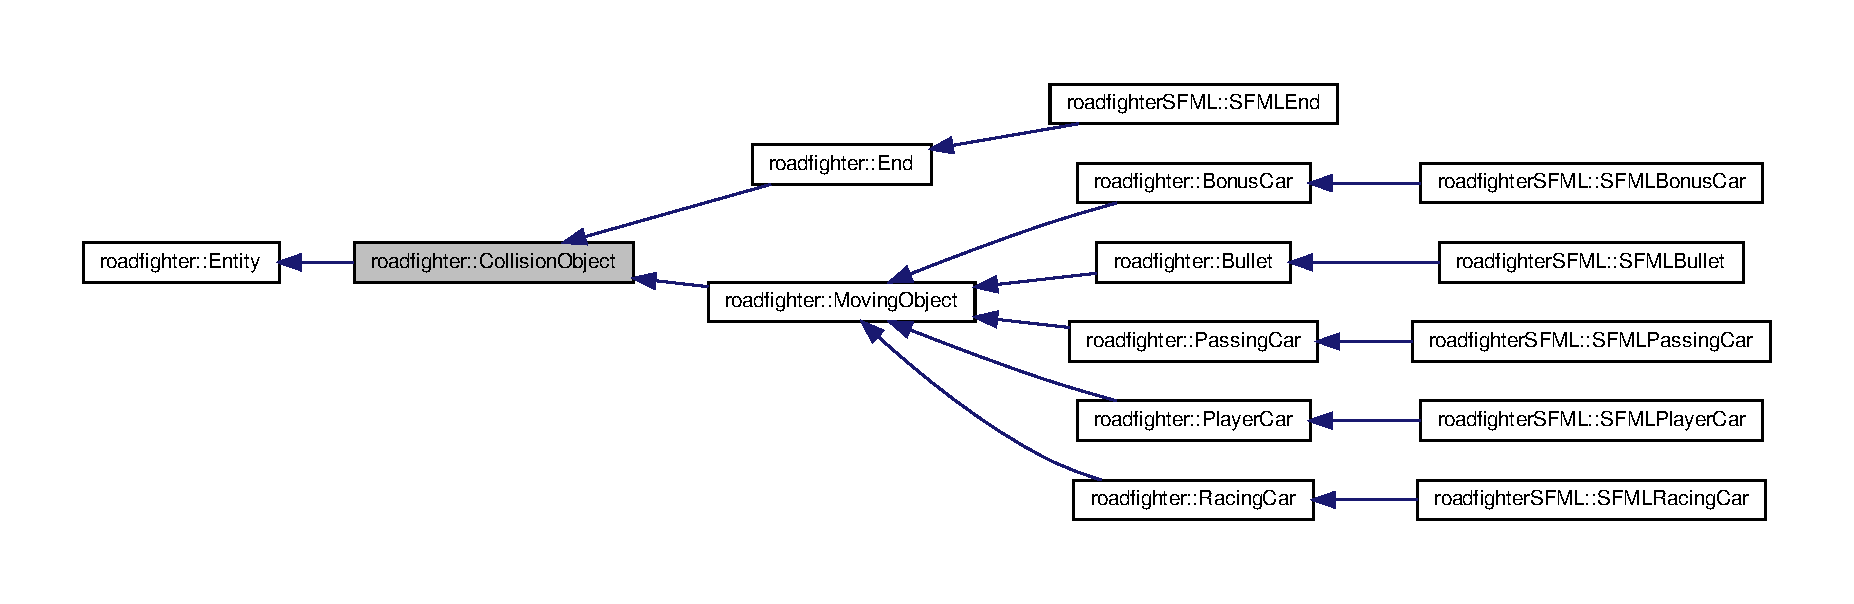
\includegraphics[width=350pt]{classroadfighter_1_1CollisionObject__inherit__graph}
\end{center}
\end{figure}


Collaboration diagram for roadfighter\+:\+:Collision\+Object\+:\nopagebreak
\begin{figure}[H]
\begin{center}
\leavevmode
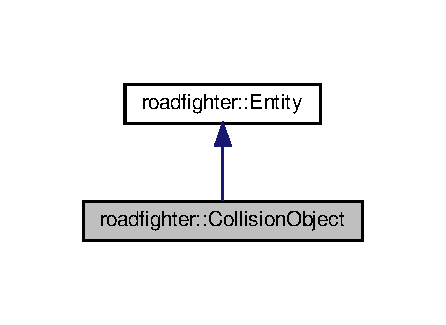
\includegraphics[width=214pt]{classroadfighter_1_1CollisionObject__coll__graph}
\end{center}
\end{figure}
\subsection*{Public Member Functions}
\begin{DoxyCompactItemize}
\item 
\hyperlink{classroadfighter_1_1CollisionObject_aa627fcee5f0f313b29d601452dadc3b0}{Collision\+Object} ()=default
\item 
\hyperlink{classroadfighter_1_1CollisionObject_a79e8e65670d1b424f1c4fadf1adde094}{Collision\+Object} (const \hyperlink{classroadfighter_1_1Location}{Location} \&m\+\_\+loc1, const \hyperlink{classroadfighter_1_1Location}{Location} \&m\+\_\+loc2)
\item 
\hyperlink{classroadfighter_1_1CollisionObject_ac19de6256e1421e1c91e98e3ba136326}{Collision\+Object} (const \hyperlink{classroadfighter_1_1CollisionObject}{Collision\+Object} \&copy)=default
\item 
\hyperlink{classroadfighter_1_1CollisionObject_a45af317bbabd99cf64e0ba87241df509}{Collision\+Object} (\hyperlink{classroadfighter_1_1CollisionObject}{Collision\+Object} \&\&move)=default
\item 
\hyperlink{classroadfighter_1_1CollisionObject}{Collision\+Object} \& \hyperlink{classroadfighter_1_1CollisionObject_a880034efde5a30ccc98c2ff3a2dc7c84}{operator=} (const \hyperlink{classroadfighter_1_1CollisionObject}{Collision\+Object} \&other)=default
\item 
\hyperlink{classroadfighter_1_1CollisionObject}{Collision\+Object} \& \hyperlink{classroadfighter_1_1CollisionObject_a68b62353ad431b65f2dbacee983b6660}{operator=} (\hyperlink{classroadfighter_1_1CollisionObject}{Collision\+Object} \&\&other)=default
\item 
virtual \hyperlink{classroadfighter_1_1CollisionObject_aabc3bc7bef3a50923856fd82e39f59a1}{$\sim$\+Collision\+Object} ()=default
\item 
virtual bool \hyperlink{classroadfighter_1_1CollisionObject_a738071cd7b1b8cd4c8d455b5e552bd4c}{must\+Delete} () const
\item 
const \hyperlink{classroadfighter_1_1Location}{Location} \& \hyperlink{classroadfighter_1_1CollisionObject_a73baa1faea7a399a944e6a6f1d04ad86}{get\+Loc1} () const
\item 
void \hyperlink{classroadfighter_1_1CollisionObject_a3e0d924b453c9003a4992046fa3c52e1}{set\+Loc1} (const \hyperlink{classroadfighter_1_1Location}{Location} \&m\+\_\+loc1)
\item 
const \hyperlink{classroadfighter_1_1Location}{Location} \& \hyperlink{classroadfighter_1_1CollisionObject_aa7412cf56663bc98b1454a8ae54ac2b0}{get\+Loc2} () const
\item 
void \hyperlink{classroadfighter_1_1CollisionObject_a8f566d1ea28f2ed16723572617abd583}{set\+Loc2} (const \hyperlink{classroadfighter_1_1Location}{Location} \&m\+\_\+loc2)
\item 
bool \hyperlink{classroadfighter_1_1CollisionObject_a426a06907212c866a22cba7ec84ebe65}{check\+Collision} (std\+::shared\+\_\+ptr$<$ \hyperlink{classroadfighter_1_1CollisionObject}{Collision\+Object} $>$ \&check) const
\item 
virtual void \hyperlink{classroadfighter_1_1CollisionObject_a9eba85551432f548f2a0c20217a60f42}{collide\+With} (std\+::shared\+\_\+ptr$<$ \hyperlink{classroadfighter_1_1CollisionObject}{Collision\+Object} $>$ \&collided)
\item 
virtual void \hyperlink{classroadfighter_1_1CollisionObject_a9a5265d810f0ed7583b60046ab3fa88c}{crash} ()
\item 
virtual void \hyperlink{classroadfighter_1_1CollisionObject_a55d891b6d9b50abdc44f964a40a7777c}{shot} ()
\item 
virtual void \hyperlink{classroadfighter_1_1CollisionObject_ad35887bb3cfb8c054eaaee56306d6944}{bonus} ()
\item 
virtual void \hyperlink{classroadfighter_1_1CollisionObject_aa793e1b9943ee90bbb4129ddd06b9be7}{win} ()
\item 
bool \hyperlink{classroadfighter_1_1CollisionObject_a2891183d9769adbc9a9c0dc65db1af10}{is\+Delete} () const
\item 
void \hyperlink{classroadfighter_1_1CollisionObject_a454547da963cd4d7e09f57bc64a0f984}{set\+Delete} (bool m\+\_\+delete)
\item 
void \hyperlink{classroadfighter_1_1CollisionObject_aaf92d0fe335daa016b5131835602bc1d}{vert\+Move} (double amount)
\item 
void \hyperlink{classroadfighter_1_1CollisionObject_a907fbb9f4a45996690b4f35bc4256e47}{hor\+Move} (double amount)
\item 
double \hyperlink{classroadfighter_1_1CollisionObject_a0c83b40afb7be4ed3b501a79c2a81b9b}{getheight} () const
\item 
double \hyperlink{classroadfighter_1_1CollisionObject_ab8692ffb0324d39a96f31c780f7a8172}{get\+Width} () const
\item 
bool \hyperlink{classroadfighter_1_1CollisionObject_ad93e53a2b4fdc7c7882a566b74cecfad}{operator==} (const \hyperlink{classroadfighter_1_1CollisionObject}{Collision\+Object} \&rhs) const
\item 
bool \hyperlink{classroadfighter_1_1CollisionObject_ada8d62684274b10fc4f19e441413da23}{operator!=} (const \hyperlink{classroadfighter_1_1CollisionObject}{Collision\+Object} \&rhs) const
\item 
bool \hyperlink{classroadfighter_1_1CollisionObject_a4e5e9b3749d6506ad037118f1ead8c53}{is\+Immune} () const
\item 
void \hyperlink{classroadfighter_1_1CollisionObject_a5be38a4125e25e85ff094aeca94c7d8e}{set\+Immune} (bool immune)
\end{DoxyCompactItemize}


\subsection{Constructor \& Destructor Documentation}
\mbox{\Hypertarget{classroadfighter_1_1CollisionObject_aa627fcee5f0f313b29d601452dadc3b0}\label{classroadfighter_1_1CollisionObject_aa627fcee5f0f313b29d601452dadc3b0}} 
\index{roadfighter\+::\+Collision\+Object@{roadfighter\+::\+Collision\+Object}!Collision\+Object@{Collision\+Object}}
\index{Collision\+Object@{Collision\+Object}!roadfighter\+::\+Collision\+Object@{roadfighter\+::\+Collision\+Object}}
\subsubsection{\texorpdfstring{Collision\+Object()}{CollisionObject()}\hspace{0.1cm}{\footnotesize\ttfamily [1/4]}}
{\footnotesize\ttfamily roadfighter\+::\+Collision\+Object\+::\+Collision\+Object (\begin{DoxyParamCaption}{ }\end{DoxyParamCaption})\hspace{0.3cm}{\ttfamily [default]}}

default constructor for \hyperlink{classroadfighter_1_1CollisionObject}{Collision\+Object} \mbox{\Hypertarget{classroadfighter_1_1CollisionObject_a79e8e65670d1b424f1c4fadf1adde094}\label{classroadfighter_1_1CollisionObject_a79e8e65670d1b424f1c4fadf1adde094}} 
\index{roadfighter\+::\+Collision\+Object@{roadfighter\+::\+Collision\+Object}!Collision\+Object@{Collision\+Object}}
\index{Collision\+Object@{Collision\+Object}!roadfighter\+::\+Collision\+Object@{roadfighter\+::\+Collision\+Object}}
\subsubsection{\texorpdfstring{Collision\+Object()}{CollisionObject()}\hspace{0.1cm}{\footnotesize\ttfamily [2/4]}}
{\footnotesize\ttfamily roadfighter\+::\+Collision\+Object\+::\+Collision\+Object (\begin{DoxyParamCaption}\item[{const \hyperlink{classroadfighter_1_1Location}{Location} \&}]{m\+\_\+loc1,  }\item[{const \hyperlink{classroadfighter_1_1Location}{Location} \&}]{m\+\_\+loc2 }\end{DoxyParamCaption})}

a non default constructor for collision\+Object where both positions are given 
\begin{DoxyParams}{Parameters}
{\em m\+\_\+loc1} & first location \\
\hline
{\em m\+\_\+loc2} & second location \\
\hline
\end{DoxyParams}
\begin{DoxyReturn}{Returns}
none 
\end{DoxyReturn}

\begin{DoxyExceptions}{Exceptions}
{\em none} & \\
\hline
\end{DoxyExceptions}
\mbox{\Hypertarget{classroadfighter_1_1CollisionObject_ac19de6256e1421e1c91e98e3ba136326}\label{classroadfighter_1_1CollisionObject_ac19de6256e1421e1c91e98e3ba136326}} 
\index{roadfighter\+::\+Collision\+Object@{roadfighter\+::\+Collision\+Object}!Collision\+Object@{Collision\+Object}}
\index{Collision\+Object@{Collision\+Object}!roadfighter\+::\+Collision\+Object@{roadfighter\+::\+Collision\+Object}}
\subsubsection{\texorpdfstring{Collision\+Object()}{CollisionObject()}\hspace{0.1cm}{\footnotesize\ttfamily [3/4]}}
{\footnotesize\ttfamily roadfighter\+::\+Collision\+Object\+::\+Collision\+Object (\begin{DoxyParamCaption}\item[{const \hyperlink{classroadfighter_1_1CollisionObject}{Collision\+Object} \&}]{copy }\end{DoxyParamCaption})\hspace{0.3cm}{\ttfamily [default]}}

copy constructor 
\begin{DoxyParams}{Parameters}
{\em copy} & the other \hyperlink{classroadfighter_1_1CollisionObject}{Collision\+Object} that is being copied \\
\hline
\end{DoxyParams}
\mbox{\Hypertarget{classroadfighter_1_1CollisionObject_a45af317bbabd99cf64e0ba87241df509}\label{classroadfighter_1_1CollisionObject_a45af317bbabd99cf64e0ba87241df509}} 
\index{roadfighter\+::\+Collision\+Object@{roadfighter\+::\+Collision\+Object}!Collision\+Object@{Collision\+Object}}
\index{Collision\+Object@{Collision\+Object}!roadfighter\+::\+Collision\+Object@{roadfighter\+::\+Collision\+Object}}
\subsubsection{\texorpdfstring{Collision\+Object()}{CollisionObject()}\hspace{0.1cm}{\footnotesize\ttfamily [4/4]}}
{\footnotesize\ttfamily roadfighter\+::\+Collision\+Object\+::\+Collision\+Object (\begin{DoxyParamCaption}\item[{\hyperlink{classroadfighter_1_1CollisionObject}{Collision\+Object} \&\&}]{move }\end{DoxyParamCaption})\hspace{0.3cm}{\ttfamily [default]}}

move constructor 
\begin{DoxyParams}{Parameters}
{\em Move} & the other \hyperlink{classroadfighter_1_1CollisionObject}{Collision\+Object} that is being moved in this one \\
\hline
\end{DoxyParams}
\mbox{\Hypertarget{classroadfighter_1_1CollisionObject_aabc3bc7bef3a50923856fd82e39f59a1}\label{classroadfighter_1_1CollisionObject_aabc3bc7bef3a50923856fd82e39f59a1}} 
\index{roadfighter\+::\+Collision\+Object@{roadfighter\+::\+Collision\+Object}!````~Collision\+Object@{$\sim$\+Collision\+Object}}
\index{````~Collision\+Object@{$\sim$\+Collision\+Object}!roadfighter\+::\+Collision\+Object@{roadfighter\+::\+Collision\+Object}}
\subsubsection{\texorpdfstring{$\sim$\+Collision\+Object()}{~CollisionObject()}}
{\footnotesize\ttfamily virtual roadfighter\+::\+Collision\+Object\+::$\sim$\+Collision\+Object (\begin{DoxyParamCaption}{ }\end{DoxyParamCaption})\hspace{0.3cm}{\ttfamily [virtual]}, {\ttfamily [default]}}

destructor for \hyperlink{classroadfighter_1_1CollisionObject}{Collision\+Object} 

\subsection{Member Function Documentation}
\mbox{\Hypertarget{classroadfighter_1_1CollisionObject_ad35887bb3cfb8c054eaaee56306d6944}\label{classroadfighter_1_1CollisionObject_ad35887bb3cfb8c054eaaee56306d6944}} 
\index{roadfighter\+::\+Collision\+Object@{roadfighter\+::\+Collision\+Object}!bonus@{bonus}}
\index{bonus@{bonus}!roadfighter\+::\+Collision\+Object@{roadfighter\+::\+Collision\+Object}}
\subsubsection{\texorpdfstring{bonus()}{bonus()}}
{\footnotesize\ttfamily virtual void roadfighter\+::\+Collision\+Object\+::bonus (\begin{DoxyParamCaption}{ }\end{DoxyParamCaption})\hspace{0.3cm}{\ttfamily [inline]}, {\ttfamily [virtual]}}

a function that can be overriden that will say what the object will do must it get a bonus it will do nothing by default 

Reimplemented in \hyperlink{classroadfighter_1_1PlayerCar_a0f0626a6ea7d25e3ba01a8289d54acac}{roadfighter\+::\+Player\+Car}, \hyperlink{classroadfighter_1_1RacingCar_a5858dd3f2c7bb49782b29c0a90846a6c}{roadfighter\+::\+Racing\+Car}, \hyperlink{classroadfighter_1_1Bullet_a642ca8467a0ffea844d18d4917b2f49e}{roadfighter\+::\+Bullet}, \hyperlink{classroadfighter_1_1BonusCar_a3d2d15df036c419cd9ad4fbc6fcd4ad9}{roadfighter\+::\+Bonus\+Car}, and \hyperlink{classroadfighter_1_1PassingCar_a43d55e28efe840d81c1b87216920eb69}{roadfighter\+::\+Passing\+Car}.

\mbox{\Hypertarget{classroadfighter_1_1CollisionObject_a426a06907212c866a22cba7ec84ebe65}\label{classroadfighter_1_1CollisionObject_a426a06907212c866a22cba7ec84ebe65}} 
\index{roadfighter\+::\+Collision\+Object@{roadfighter\+::\+Collision\+Object}!check\+Collision@{check\+Collision}}
\index{check\+Collision@{check\+Collision}!roadfighter\+::\+Collision\+Object@{roadfighter\+::\+Collision\+Object}}
\subsubsection{\texorpdfstring{check\+Collision()}{checkCollision()}}
{\footnotesize\ttfamily bool roadfighter\+::\+Collision\+Object\+::check\+Collision (\begin{DoxyParamCaption}\item[{std\+::shared\+\_\+ptr$<$ \hyperlink{classroadfighter_1_1CollisionObject}{Collision\+Object} $>$ \&}]{check }\end{DoxyParamCaption}) const}

this function checks whether 2 collisionobjects collide 
\begin{DoxyParams}{Parameters}
{\em check} & the collisionobject you are checking with \\
\hline
\end{DoxyParams}
\begin{DoxyReturn}{Returns}
a bool that is true if they collide 
\end{DoxyReturn}

\begin{DoxyExceptions}{Exceptions}
{\em none} & \\
\hline
\end{DoxyExceptions}
\mbox{\Hypertarget{classroadfighter_1_1CollisionObject_a9eba85551432f548f2a0c20217a60f42}\label{classroadfighter_1_1CollisionObject_a9eba85551432f548f2a0c20217a60f42}} 
\index{roadfighter\+::\+Collision\+Object@{roadfighter\+::\+Collision\+Object}!collide\+With@{collide\+With}}
\index{collide\+With@{collide\+With}!roadfighter\+::\+Collision\+Object@{roadfighter\+::\+Collision\+Object}}
\subsubsection{\texorpdfstring{collide\+With()}{collideWith()}}
{\footnotesize\ttfamily virtual void roadfighter\+::\+Collision\+Object\+::collide\+With (\begin{DoxyParamCaption}\item[{std\+::shared\+\_\+ptr$<$ \hyperlink{classroadfighter_1_1CollisionObject}{Collision\+Object} $>$ \&}]{collided }\end{DoxyParamCaption})\hspace{0.3cm}{\ttfamily [inline]}, {\ttfamily [virtual]}}

a function that can be overriden that will say what will happen to an object must it collide with this one 
\begin{DoxyParams}{Parameters}
{\em collided} & the object this one collided with it will do nothing by default \\
\hline
\end{DoxyParams}


Reimplemented in \hyperlink{classroadfighter_1_1PlayerCar_ab62e40d949ac12f402fdaaab15c69b81}{roadfighter\+::\+Player\+Car}, \hyperlink{classroadfighter_1_1RacingCar_a1de00cf7c8df548e8ab57a27cefb7345}{roadfighter\+::\+Racing\+Car}, \hyperlink{classroadfighter_1_1Bullet_a36156632331e59c11abf5ae76024bc1f}{roadfighter\+::\+Bullet}, \hyperlink{classroadfighter_1_1BonusCar_ad1ce65b53e5652eac482a7b00c9a1d51}{roadfighter\+::\+Bonus\+Car}, \hyperlink{classroadfighter_1_1PassingCar_a04ee71b75c90f21efef591756855bf37}{roadfighter\+::\+Passing\+Car}, and \hyperlink{classroadfighter_1_1End_a56dfbe6f0c760a5728b58fc9d9f40486}{roadfighter\+::\+End}.

\mbox{\Hypertarget{classroadfighter_1_1CollisionObject_a9a5265d810f0ed7583b60046ab3fa88c}\label{classroadfighter_1_1CollisionObject_a9a5265d810f0ed7583b60046ab3fa88c}} 
\index{roadfighter\+::\+Collision\+Object@{roadfighter\+::\+Collision\+Object}!crash@{crash}}
\index{crash@{crash}!roadfighter\+::\+Collision\+Object@{roadfighter\+::\+Collision\+Object}}
\subsubsection{\texorpdfstring{crash()}{crash()}}
{\footnotesize\ttfamily virtual void roadfighter\+::\+Collision\+Object\+::crash (\begin{DoxyParamCaption}{ }\end{DoxyParamCaption})\hspace{0.3cm}{\ttfamily [inline]}, {\ttfamily [virtual]}}

a function that can be overriden that will say what the object will do must it crash it will do nothing by default 

Reimplemented in \hyperlink{classroadfighter_1_1PlayerCar_a330d071af729d7afbfcfd7ef92516544}{roadfighter\+::\+Player\+Car}, \hyperlink{classroadfighter_1_1RacingCar_a2f5018f17852d75682afd78e806b8e4c}{roadfighter\+::\+Racing\+Car}, \hyperlink{classroadfighter_1_1Bullet_ac96121377fffa9ed8ea94c333a841a7a}{roadfighter\+::\+Bullet}, \hyperlink{classroadfighter_1_1BonusCar_aad0a2a41a1b84c6487c1fc204b5f7cb7}{roadfighter\+::\+Bonus\+Car}, and \hyperlink{classroadfighter_1_1PassingCar_a5c437fb5164d2735881a469650db048d}{roadfighter\+::\+Passing\+Car}.

\mbox{\Hypertarget{classroadfighter_1_1CollisionObject_a0c83b40afb7be4ed3b501a79c2a81b9b}\label{classroadfighter_1_1CollisionObject_a0c83b40afb7be4ed3b501a79c2a81b9b}} 
\index{roadfighter\+::\+Collision\+Object@{roadfighter\+::\+Collision\+Object}!getheight@{getheight}}
\index{getheight@{getheight}!roadfighter\+::\+Collision\+Object@{roadfighter\+::\+Collision\+Object}}
\subsubsection{\texorpdfstring{getheight()}{getheight()}}
{\footnotesize\ttfamily double roadfighter\+::\+Collision\+Object\+::getheight (\begin{DoxyParamCaption}{ }\end{DoxyParamCaption}) const}

this function calculates and returns the height of the object \begin{DoxyReturn}{Returns}
a double 
\end{DoxyReturn}

\begin{DoxyExceptions}{Exceptions}
{\em none} & \\
\hline
\end{DoxyExceptions}
\mbox{\Hypertarget{classroadfighter_1_1CollisionObject_a73baa1faea7a399a944e6a6f1d04ad86}\label{classroadfighter_1_1CollisionObject_a73baa1faea7a399a944e6a6f1d04ad86}} 
\index{roadfighter\+::\+Collision\+Object@{roadfighter\+::\+Collision\+Object}!get\+Loc1@{get\+Loc1}}
\index{get\+Loc1@{get\+Loc1}!roadfighter\+::\+Collision\+Object@{roadfighter\+::\+Collision\+Object}}
\subsubsection{\texorpdfstring{get\+Loc1()}{getLoc1()}}
{\footnotesize\ttfamily const \hyperlink{classroadfighter_1_1Location}{Location} \& roadfighter\+::\+Collision\+Object\+::get\+Loc1 (\begin{DoxyParamCaption}{ }\end{DoxyParamCaption}) const}

getter for loc1 \begin{DoxyReturn}{Returns}
a gamelocation 
\end{DoxyReturn}

\begin{DoxyExceptions}{Exceptions}
{\em none} & \\
\hline
\end{DoxyExceptions}
\mbox{\Hypertarget{classroadfighter_1_1CollisionObject_aa7412cf56663bc98b1454a8ae54ac2b0}\label{classroadfighter_1_1CollisionObject_aa7412cf56663bc98b1454a8ae54ac2b0}} 
\index{roadfighter\+::\+Collision\+Object@{roadfighter\+::\+Collision\+Object}!get\+Loc2@{get\+Loc2}}
\index{get\+Loc2@{get\+Loc2}!roadfighter\+::\+Collision\+Object@{roadfighter\+::\+Collision\+Object}}
\subsubsection{\texorpdfstring{get\+Loc2()}{getLoc2()}}
{\footnotesize\ttfamily const \hyperlink{classroadfighter_1_1Location}{Location} \& roadfighter\+::\+Collision\+Object\+::get\+Loc2 (\begin{DoxyParamCaption}{ }\end{DoxyParamCaption}) const}

getter for loc2 \begin{DoxyReturn}{Returns}
a gamelocation 
\end{DoxyReturn}

\begin{DoxyExceptions}{Exceptions}
{\em none} & \\
\hline
\end{DoxyExceptions}
\mbox{\Hypertarget{classroadfighter_1_1CollisionObject_ab8692ffb0324d39a96f31c780f7a8172}\label{classroadfighter_1_1CollisionObject_ab8692ffb0324d39a96f31c780f7a8172}} 
\index{roadfighter\+::\+Collision\+Object@{roadfighter\+::\+Collision\+Object}!get\+Width@{get\+Width}}
\index{get\+Width@{get\+Width}!roadfighter\+::\+Collision\+Object@{roadfighter\+::\+Collision\+Object}}
\subsubsection{\texorpdfstring{get\+Width()}{getWidth()}}
{\footnotesize\ttfamily double roadfighter\+::\+Collision\+Object\+::get\+Width (\begin{DoxyParamCaption}{ }\end{DoxyParamCaption}) const}

this function calculates and returns the width of the object \begin{DoxyReturn}{Returns}
a double 
\end{DoxyReturn}

\begin{DoxyExceptions}{Exceptions}
{\em none} & \\
\hline
\end{DoxyExceptions}
\mbox{\Hypertarget{classroadfighter_1_1CollisionObject_a907fbb9f4a45996690b4f35bc4256e47}\label{classroadfighter_1_1CollisionObject_a907fbb9f4a45996690b4f35bc4256e47}} 
\index{roadfighter\+::\+Collision\+Object@{roadfighter\+::\+Collision\+Object}!hor\+Move@{hor\+Move}}
\index{hor\+Move@{hor\+Move}!roadfighter\+::\+Collision\+Object@{roadfighter\+::\+Collision\+Object}}
\subsubsection{\texorpdfstring{hor\+Move()}{horMove()}}
{\footnotesize\ttfamily void roadfighter\+::\+Collision\+Object\+::hor\+Move (\begin{DoxyParamCaption}\item[{double}]{amount }\end{DoxyParamCaption})}

function that moves the collisionobject horizontaly 
\begin{DoxyParams}{Parameters}
{\em amount} & the amount it must forward/backward \\
\hline
\end{DoxyParams}
\begin{DoxyReturn}{Returns}
none 
\end{DoxyReturn}

\begin{DoxyExceptions}{Exceptions}
{\em \hyperlink{classroadfighter_1_1GllException}{Gll\+Exception}} & \\
\hline
\end{DoxyExceptions}
\mbox{\Hypertarget{classroadfighter_1_1CollisionObject_a2891183d9769adbc9a9c0dc65db1af10}\label{classroadfighter_1_1CollisionObject_a2891183d9769adbc9a9c0dc65db1af10}} 
\index{roadfighter\+::\+Collision\+Object@{roadfighter\+::\+Collision\+Object}!is\+Delete@{is\+Delete}}
\index{is\+Delete@{is\+Delete}!roadfighter\+::\+Collision\+Object@{roadfighter\+::\+Collision\+Object}}
\subsubsection{\texorpdfstring{is\+Delete()}{isDelete()}}
{\footnotesize\ttfamily bool roadfighter\+::\+Collision\+Object\+::is\+Delete (\begin{DoxyParamCaption}{ }\end{DoxyParamCaption}) const}

getter for m\+\_\+delete \begin{DoxyReturn}{Returns}
a bool 
\end{DoxyReturn}

\begin{DoxyExceptions}{Exceptions}
{\em none} & \\
\hline
\end{DoxyExceptions}
\mbox{\Hypertarget{classroadfighter_1_1CollisionObject_a4e5e9b3749d6506ad037118f1ead8c53}\label{classroadfighter_1_1CollisionObject_a4e5e9b3749d6506ad037118f1ead8c53}} 
\index{roadfighter\+::\+Collision\+Object@{roadfighter\+::\+Collision\+Object}!is\+Immune@{is\+Immune}}
\index{is\+Immune@{is\+Immune}!roadfighter\+::\+Collision\+Object@{roadfighter\+::\+Collision\+Object}}
\subsubsection{\texorpdfstring{is\+Immune()}{isImmune()}}
{\footnotesize\ttfamily bool roadfighter\+::\+Collision\+Object\+::is\+Immune (\begin{DoxyParamCaption}{ }\end{DoxyParamCaption}) const}

a getter for the immunity of the object \begin{DoxyReturn}{Returns}
a bool 
\end{DoxyReturn}

\begin{DoxyExceptions}{Exceptions}
{\em none} & \\
\hline
\end{DoxyExceptions}
\mbox{\Hypertarget{classroadfighter_1_1CollisionObject_a738071cd7b1b8cd4c8d455b5e552bd4c}\label{classroadfighter_1_1CollisionObject_a738071cd7b1b8cd4c8d455b5e552bd4c}} 
\index{roadfighter\+::\+Collision\+Object@{roadfighter\+::\+Collision\+Object}!must\+Delete@{must\+Delete}}
\index{must\+Delete@{must\+Delete}!roadfighter\+::\+Collision\+Object@{roadfighter\+::\+Collision\+Object}}
\subsubsection{\texorpdfstring{must\+Delete()}{mustDelete()}}
{\footnotesize\ttfamily bool roadfighter\+::\+Collision\+Object\+::must\+Delete (\begin{DoxyParamCaption}{ }\end{DoxyParamCaption}) const\hspace{0.3cm}{\ttfamily [virtual]}}

a function that should be overriden and is used to denote whether an object should be deleted or not \begin{DoxyReturn}{Returns}
a bool 
\end{DoxyReturn}

\begin{DoxyExceptions}{Exceptions}
{\em none} & \\
\hline
\end{DoxyExceptions}


Reimplemented in \hyperlink{classroadfighter_1_1Bullet_a0f87b693a1583522e551ba1324fcd067}{roadfighter\+::\+Bullet}, \hyperlink{classroadfighter_1_1PlayerCar_aaf4dc181a4d21e544aecd7a8e538cfd6}{roadfighter\+::\+Player\+Car}, \hyperlink{classroadfighter_1_1RacingCar_a300bccb330cc8e84834edd5f85354a10}{roadfighter\+::\+Racing\+Car}, \hyperlink{classroadfighter_1_1BonusCar_a19d01e92134634a82ae53f0d017956aa}{roadfighter\+::\+Bonus\+Car}, and \hyperlink{classroadfighter_1_1PassingCar_a96b365c19d4e6e940d3827319434a022}{roadfighter\+::\+Passing\+Car}.

\mbox{\Hypertarget{classroadfighter_1_1CollisionObject_ada8d62684274b10fc4f19e441413da23}\label{classroadfighter_1_1CollisionObject_ada8d62684274b10fc4f19e441413da23}} 
\index{roadfighter\+::\+Collision\+Object@{roadfighter\+::\+Collision\+Object}!operator"!=@{operator"!=}}
\index{operator"!=@{operator"!=}!roadfighter\+::\+Collision\+Object@{roadfighter\+::\+Collision\+Object}}
\subsubsection{\texorpdfstring{operator"!=()}{operator!=()}}
{\footnotesize\ttfamily bool roadfighter\+::\+Collision\+Object\+::operator!= (\begin{DoxyParamCaption}\item[{const \hyperlink{classroadfighter_1_1CollisionObject}{Collision\+Object} \&}]{rhs }\end{DoxyParamCaption}) const}

unequality operator 
\begin{DoxyParams}{Parameters}
{\em rhs} & object you are comparing to \\
\hline
\end{DoxyParams}
\begin{DoxyReturn}{Returns}
bool that says whether they are not equal or equal 
\end{DoxyReturn}
\mbox{\Hypertarget{classroadfighter_1_1CollisionObject_a880034efde5a30ccc98c2ff3a2dc7c84}\label{classroadfighter_1_1CollisionObject_a880034efde5a30ccc98c2ff3a2dc7c84}} 
\index{roadfighter\+::\+Collision\+Object@{roadfighter\+::\+Collision\+Object}!operator=@{operator=}}
\index{operator=@{operator=}!roadfighter\+::\+Collision\+Object@{roadfighter\+::\+Collision\+Object}}
\subsubsection{\texorpdfstring{operator=()}{operator=()}\hspace{0.1cm}{\footnotesize\ttfamily [1/2]}}
{\footnotesize\ttfamily \hyperlink{classroadfighter_1_1CollisionObject}{Collision\+Object}\& roadfighter\+::\+Collision\+Object\+::operator= (\begin{DoxyParamCaption}\item[{const \hyperlink{classroadfighter_1_1CollisionObject}{Collision\+Object} \&}]{other }\end{DoxyParamCaption})\hspace{0.3cm}{\ttfamily [default]}}

copy assigment for \hyperlink{classroadfighter_1_1CollisionObject}{Collision\+Object} 
\begin{DoxyParams}{Parameters}
{\em other} & the \hyperlink{classroadfighter_1_1CollisionObject}{Collision\+Object} that is being copied \\
\hline
\end{DoxyParams}
\begin{DoxyReturn}{Returns}
a new \hyperlink{classroadfighter_1_1CollisionObject}{Collision\+Object} that is equal to the other one 
\end{DoxyReturn}
\mbox{\Hypertarget{classroadfighter_1_1CollisionObject_a68b62353ad431b65f2dbacee983b6660}\label{classroadfighter_1_1CollisionObject_a68b62353ad431b65f2dbacee983b6660}} 
\index{roadfighter\+::\+Collision\+Object@{roadfighter\+::\+Collision\+Object}!operator=@{operator=}}
\index{operator=@{operator=}!roadfighter\+::\+Collision\+Object@{roadfighter\+::\+Collision\+Object}}
\subsubsection{\texorpdfstring{operator=()}{operator=()}\hspace{0.1cm}{\footnotesize\ttfamily [2/2]}}
{\footnotesize\ttfamily \hyperlink{classroadfighter_1_1CollisionObject}{Collision\+Object}\& roadfighter\+::\+Collision\+Object\+::operator= (\begin{DoxyParamCaption}\item[{\hyperlink{classroadfighter_1_1CollisionObject}{Collision\+Object} \&\&}]{other }\end{DoxyParamCaption})\hspace{0.3cm}{\ttfamily [default]}}

move assignment for \hyperlink{classroadfighter_1_1CollisionObject}{Collision\+Object} 
\begin{DoxyParams}{Parameters}
{\em other} & other \hyperlink{classroadfighter_1_1CollisionObject}{Collision\+Object} that is being moved \\
\hline
\end{DoxyParams}
\begin{DoxyReturn}{Returns}
a \hyperlink{classroadfighter_1_1CollisionObject}{Collision\+Object} that contains all the data of the first one 
\end{DoxyReturn}
\mbox{\Hypertarget{classroadfighter_1_1CollisionObject_ad93e53a2b4fdc7c7882a566b74cecfad}\label{classroadfighter_1_1CollisionObject_ad93e53a2b4fdc7c7882a566b74cecfad}} 
\index{roadfighter\+::\+Collision\+Object@{roadfighter\+::\+Collision\+Object}!operator==@{operator==}}
\index{operator==@{operator==}!roadfighter\+::\+Collision\+Object@{roadfighter\+::\+Collision\+Object}}
\subsubsection{\texorpdfstring{operator==()}{operator==()}}
{\footnotesize\ttfamily bool roadfighter\+::\+Collision\+Object\+::operator== (\begin{DoxyParamCaption}\item[{const \hyperlink{classroadfighter_1_1CollisionObject}{Collision\+Object} \&}]{rhs }\end{DoxyParamCaption}) const}

equality operator 
\begin{DoxyParams}{Parameters}
{\em rhs} & object you are comparing to \\
\hline
\end{DoxyParams}
\begin{DoxyReturn}{Returns}
bool that says whether they are equal or not 
\end{DoxyReturn}
\mbox{\Hypertarget{classroadfighter_1_1CollisionObject_a454547da963cd4d7e09f57bc64a0f984}\label{classroadfighter_1_1CollisionObject_a454547da963cd4d7e09f57bc64a0f984}} 
\index{roadfighter\+::\+Collision\+Object@{roadfighter\+::\+Collision\+Object}!set\+Delete@{set\+Delete}}
\index{set\+Delete@{set\+Delete}!roadfighter\+::\+Collision\+Object@{roadfighter\+::\+Collision\+Object}}
\subsubsection{\texorpdfstring{set\+Delete()}{setDelete()}}
{\footnotesize\ttfamily void roadfighter\+::\+Collision\+Object\+::set\+Delete (\begin{DoxyParamCaption}\item[{bool}]{m\+\_\+delete }\end{DoxyParamCaption})}

setter for m\+\_\+delete 
\begin{DoxyParams}{Parameters}
{\em m\+\_\+delete} & a bool \\
\hline
\end{DoxyParams}
\begin{DoxyReturn}{Returns}
none 
\end{DoxyReturn}

\begin{DoxyExceptions}{Exceptions}
{\em none} & \\
\hline
\end{DoxyExceptions}
\mbox{\Hypertarget{classroadfighter_1_1CollisionObject_a5be38a4125e25e85ff094aeca94c7d8e}\label{classroadfighter_1_1CollisionObject_a5be38a4125e25e85ff094aeca94c7d8e}} 
\index{roadfighter\+::\+Collision\+Object@{roadfighter\+::\+Collision\+Object}!set\+Immune@{set\+Immune}}
\index{set\+Immune@{set\+Immune}!roadfighter\+::\+Collision\+Object@{roadfighter\+::\+Collision\+Object}}
\subsubsection{\texorpdfstring{set\+Immune()}{setImmune()}}
{\footnotesize\ttfamily void roadfighter\+::\+Collision\+Object\+::set\+Immune (\begin{DoxyParamCaption}\item[{bool}]{immune }\end{DoxyParamCaption})}

setter for the immunity of the object 
\begin{DoxyParams}{Parameters}
{\em immune} & a bool \\
\hline
\end{DoxyParams}
\begin{DoxyReturn}{Returns}
none 
\end{DoxyReturn}

\begin{DoxyExceptions}{Exceptions}
{\em none} & \\
\hline
\end{DoxyExceptions}
\mbox{\Hypertarget{classroadfighter_1_1CollisionObject_a3e0d924b453c9003a4992046fa3c52e1}\label{classroadfighter_1_1CollisionObject_a3e0d924b453c9003a4992046fa3c52e1}} 
\index{roadfighter\+::\+Collision\+Object@{roadfighter\+::\+Collision\+Object}!set\+Loc1@{set\+Loc1}}
\index{set\+Loc1@{set\+Loc1}!roadfighter\+::\+Collision\+Object@{roadfighter\+::\+Collision\+Object}}
\subsubsection{\texorpdfstring{set\+Loc1()}{setLoc1()}}
{\footnotesize\ttfamily void roadfighter\+::\+Collision\+Object\+::set\+Loc1 (\begin{DoxyParamCaption}\item[{const \hyperlink{classroadfighter_1_1Location}{Location} \&}]{m\+\_\+loc1 }\end{DoxyParamCaption})}

setter for loc1 
\begin{DoxyParams}{Parameters}
{\em m\+\_\+loc1} & a gamelocation \\
\hline
\end{DoxyParams}
\begin{DoxyReturn}{Returns}
none 
\end{DoxyReturn}

\begin{DoxyExceptions}{Exceptions}
{\em none} & \\
\hline
\end{DoxyExceptions}
\mbox{\Hypertarget{classroadfighter_1_1CollisionObject_a8f566d1ea28f2ed16723572617abd583}\label{classroadfighter_1_1CollisionObject_a8f566d1ea28f2ed16723572617abd583}} 
\index{roadfighter\+::\+Collision\+Object@{roadfighter\+::\+Collision\+Object}!set\+Loc2@{set\+Loc2}}
\index{set\+Loc2@{set\+Loc2}!roadfighter\+::\+Collision\+Object@{roadfighter\+::\+Collision\+Object}}
\subsubsection{\texorpdfstring{set\+Loc2()}{setLoc2()}}
{\footnotesize\ttfamily void roadfighter\+::\+Collision\+Object\+::set\+Loc2 (\begin{DoxyParamCaption}\item[{const \hyperlink{classroadfighter_1_1Location}{Location} \&}]{m\+\_\+loc2 }\end{DoxyParamCaption})}

setter for loc2 
\begin{DoxyParams}{Parameters}
{\em m\+\_\+loc2} & a gamelocation \\
\hline
\end{DoxyParams}
\begin{DoxyReturn}{Returns}
none 
\end{DoxyReturn}

\begin{DoxyExceptions}{Exceptions}
{\em none} & \\
\hline
\end{DoxyExceptions}
\mbox{\Hypertarget{classroadfighter_1_1CollisionObject_a55d891b6d9b50abdc44f964a40a7777c}\label{classroadfighter_1_1CollisionObject_a55d891b6d9b50abdc44f964a40a7777c}} 
\index{roadfighter\+::\+Collision\+Object@{roadfighter\+::\+Collision\+Object}!shot@{shot}}
\index{shot@{shot}!roadfighter\+::\+Collision\+Object@{roadfighter\+::\+Collision\+Object}}
\subsubsection{\texorpdfstring{shot()}{shot()}}
{\footnotesize\ttfamily virtual void roadfighter\+::\+Collision\+Object\+::shot (\begin{DoxyParamCaption}{ }\end{DoxyParamCaption})\hspace{0.3cm}{\ttfamily [inline]}, {\ttfamily [virtual]}}

a function that can be overriden that will say what the object will do must it been shot it will do nothing by default 

Reimplemented in \hyperlink{classroadfighter_1_1PlayerCar_a592556a1c6326c9d9a70691f036eaafc}{roadfighter\+::\+Player\+Car}, \hyperlink{classroadfighter_1_1RacingCar_a20c4363a1d31cc17d7d82c8f9a219d2d}{roadfighter\+::\+Racing\+Car}, \hyperlink{classroadfighter_1_1Bullet_acaacd303f1f4e55c5029d4a4cbe1d9b1}{roadfighter\+::\+Bullet}, \hyperlink{classroadfighter_1_1BonusCar_a02edcd22a86c1f98642c3703ef8dfb16}{roadfighter\+::\+Bonus\+Car}, and \hyperlink{classroadfighter_1_1PassingCar_ac04b801b789bf880011d5cdb1ffdec59}{roadfighter\+::\+Passing\+Car}.

\mbox{\Hypertarget{classroadfighter_1_1CollisionObject_aaf92d0fe335daa016b5131835602bc1d}\label{classroadfighter_1_1CollisionObject_aaf92d0fe335daa016b5131835602bc1d}} 
\index{roadfighter\+::\+Collision\+Object@{roadfighter\+::\+Collision\+Object}!vert\+Move@{vert\+Move}}
\index{vert\+Move@{vert\+Move}!roadfighter\+::\+Collision\+Object@{roadfighter\+::\+Collision\+Object}}
\subsubsection{\texorpdfstring{vert\+Move()}{vertMove()}}
{\footnotesize\ttfamily void roadfighter\+::\+Collision\+Object\+::vert\+Move (\begin{DoxyParamCaption}\item[{double}]{amount }\end{DoxyParamCaption})}

this function moves the object forward/backward by \char`\"{}amount\char`\"{} space 
\begin{DoxyParams}{Parameters}
{\em amount} & the amount it is moving (negative is forward!!) \\
\hline
\end{DoxyParams}
\begin{DoxyReturn}{Returns}
none 
\end{DoxyReturn}

\begin{DoxyExceptions}{Exceptions}
{\em none} & \\
\hline
\end{DoxyExceptions}
\mbox{\Hypertarget{classroadfighter_1_1CollisionObject_aa793e1b9943ee90bbb4129ddd06b9be7}\label{classroadfighter_1_1CollisionObject_aa793e1b9943ee90bbb4129ddd06b9be7}} 
\index{roadfighter\+::\+Collision\+Object@{roadfighter\+::\+Collision\+Object}!win@{win}}
\index{win@{win}!roadfighter\+::\+Collision\+Object@{roadfighter\+::\+Collision\+Object}}
\subsubsection{\texorpdfstring{win()}{win()}}
{\footnotesize\ttfamily virtual void roadfighter\+::\+Collision\+Object\+::win (\begin{DoxyParamCaption}{ }\end{DoxyParamCaption})\hspace{0.3cm}{\ttfamily [inline]}, {\ttfamily [virtual]}}

a function that can be overriden that will say what the object will do must it win it will do nothing by default 

Reimplemented in \hyperlink{classroadfighter_1_1Bullet_a566adb0235665312365cd65536c2aafc}{roadfighter\+::\+Bullet}, \hyperlink{classroadfighter_1_1PlayerCar_a12f0da24565a4fe64a7bf17fc7c37152}{roadfighter\+::\+Player\+Car}, \hyperlink{classroadfighter_1_1BonusCar_afb2d142de799694db896ba875d7d0c27}{roadfighter\+::\+Bonus\+Car}, \hyperlink{classroadfighter_1_1PassingCar_a365d8befb1c2fd34337fc25665ccc73f}{roadfighter\+::\+Passing\+Car}, and \hyperlink{classroadfighter_1_1RacingCar_a24293ac56920da01d29fe99aee8d3ea6}{roadfighter\+::\+Racing\+Car}.



The documentation for this class was generated from the following files\+:\begin{DoxyCompactItemize}
\item 
Game\+Logic/include/\+Entities/\hyperlink{CollisionObject_8h}{Collision\+Object.\+h}\item 
Game\+Logic/\+Source/\+Entities/\hyperlink{CollisionObject_8cpp}{Collision\+Object.\+cpp}\end{DoxyCompactItemize}

\hypertarget{classroadfighter_1_1End}{}\section{roadfighter\+:\+:End Class Reference}
\label{classroadfighter_1_1End}\index{roadfighter\+::\+End@{roadfighter\+::\+End}}


Inheritance diagram for roadfighter\+:\+:End\+:
\nopagebreak
\begin{figure}[H]
\begin{center}
\leavevmode
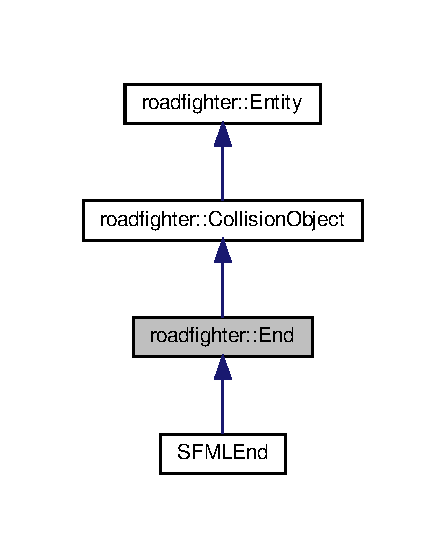
\includegraphics[width=218pt]{classroadfighter_1_1End__inherit__graph}
\end{center}
\end{figure}


Collaboration diagram for roadfighter\+:\+:End\+:\nopagebreak
\begin{figure}[H]
\begin{center}
\leavevmode
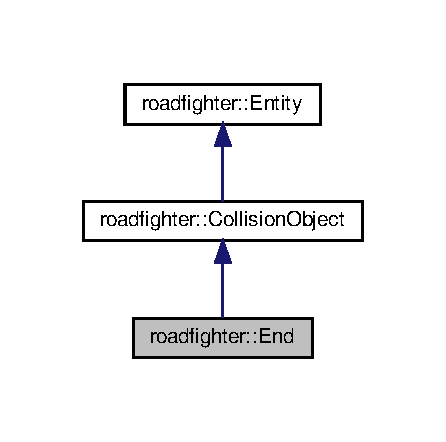
\includegraphics[width=214pt]{classroadfighter_1_1End__coll__graph}
\end{center}
\end{figure}
\subsection*{Public Member Functions}
\begin{DoxyCompactItemize}
\item 
void \hyperlink{classroadfighter_1_1End_a56dfbe6f0c760a5728b58fc9d9f40486}{collide\+With} (std\+::shared\+\_\+ptr$<$ \hyperlink{classroadfighter_1_1CollisionObject}{Collision\+Object} $>$ \&collided) override
\item 
void \hyperlink{classroadfighter_1_1End_aee4a4fed3e7bd5f85f183351280e54f9}{update\+Logic} () override
\item 
void \hyperlink{classroadfighter_1_1End_a6ea4afe8b07f96801fb2a67b82d6b71c}{update\+Movement} (double dt) override
\item 
\hyperlink{classroadfighter_1_1End_ab5806203f3fb473a220b3cce19f2fb0c}{End} (const \hyperlink{classroadfighter_1_1Location}{Location} \&m\+\_\+loc1, const \hyperlink{classroadfighter_1_1Location}{Location} \&m\+\_\+loc2)
\end{DoxyCompactItemize}


\subsection{Constructor \& Destructor Documentation}
\mbox{\Hypertarget{classroadfighter_1_1End_ab5806203f3fb473a220b3cce19f2fb0c}\label{classroadfighter_1_1End_ab5806203f3fb473a220b3cce19f2fb0c}} 
\index{roadfighter\+::\+End@{roadfighter\+::\+End}!End@{End}}
\index{End@{End}!roadfighter\+::\+End@{roadfighter\+::\+End}}
\subsubsection{\texorpdfstring{End()}{End()}}
{\footnotesize\ttfamily roadfighter\+::\+End\+::\+End (\begin{DoxyParamCaption}\item[{const \hyperlink{classroadfighter_1_1Location}{Location} \&}]{m\+\_\+loc1,  }\item[{const \hyperlink{classroadfighter_1_1Location}{Location} \&}]{m\+\_\+loc2 }\end{DoxyParamCaption})}

constructor for end where all the parameters are given 
\begin{DoxyParams}{Parameters}
{\em m\+\_\+loc1} & first location \\
\hline
{\em m\+\_\+loc2} & second location \\
\hline
\end{DoxyParams}
\begin{DoxyReturn}{Returns}
none 
\end{DoxyReturn}

\begin{DoxyExceptions}{Exceptions}
{\em none} & \\
\hline
\end{DoxyExceptions}


\subsection{Member Function Documentation}
\mbox{\Hypertarget{classroadfighter_1_1End_a56dfbe6f0c760a5728b58fc9d9f40486}\label{classroadfighter_1_1End_a56dfbe6f0c760a5728b58fc9d9f40486}} 
\index{roadfighter\+::\+End@{roadfighter\+::\+End}!collide\+With@{collide\+With}}
\index{collide\+With@{collide\+With}!roadfighter\+::\+End@{roadfighter\+::\+End}}
\subsubsection{\texorpdfstring{collide\+With()}{collideWith()}}
{\footnotesize\ttfamily void roadfighter\+::\+End\+::collide\+With (\begin{DoxyParamCaption}\item[{std\+::shared\+\_\+ptr$<$ \hyperlink{classroadfighter_1_1CollisionObject}{Collision\+Object} $>$ \&}]{collided }\end{DoxyParamCaption})\hspace{0.3cm}{\ttfamily [override]}, {\ttfamily [virtual]}}

a function that will handle what will happen when an object collides with this one 
\begin{DoxyParams}{Parameters}
{\em collided} & the object it collides with \\
\hline
\end{DoxyParams}
\begin{DoxyReturn}{Returns}
none 
\end{DoxyReturn}

\begin{DoxyExceptions}{Exceptions}
{\em none} & \\
\hline
\end{DoxyExceptions}


Reimplemented from \hyperlink{classroadfighter_1_1CollisionObject_a9eba85551432f548f2a0c20217a60f42}{roadfighter\+::\+Collision\+Object}.

\mbox{\Hypertarget{classroadfighter_1_1End_aee4a4fed3e7bd5f85f183351280e54f9}\label{classroadfighter_1_1End_aee4a4fed3e7bd5f85f183351280e54f9}} 
\index{roadfighter\+::\+End@{roadfighter\+::\+End}!update\+Logic@{update\+Logic}}
\index{update\+Logic@{update\+Logic}!roadfighter\+::\+End@{roadfighter\+::\+End}}
\subsubsection{\texorpdfstring{update\+Logic()}{updateLogic()}}
{\footnotesize\ttfamily void roadfighter\+::\+End\+::update\+Logic (\begin{DoxyParamCaption}{ }\end{DoxyParamCaption})\hspace{0.3cm}{\ttfamily [override]}, {\ttfamily [virtual]}}

this function updates the logic of the end object it does nothing because there is no logic in the end object \begin{DoxyReturn}{Returns}
none 
\end{DoxyReturn}

\begin{DoxyExceptions}{Exceptions}
{\em none} & \\
\hline
\end{DoxyExceptions}


Implements \hyperlink{classroadfighter_1_1Entity_a54c00f1af306290bae3e4b84e196566b}{roadfighter\+::\+Entity}.

\mbox{\Hypertarget{classroadfighter_1_1End_a6ea4afe8b07f96801fb2a67b82d6b71c}\label{classroadfighter_1_1End_a6ea4afe8b07f96801fb2a67b82d6b71c}} 
\index{roadfighter\+::\+End@{roadfighter\+::\+End}!update\+Movement@{update\+Movement}}
\index{update\+Movement@{update\+Movement}!roadfighter\+::\+End@{roadfighter\+::\+End}}
\subsubsection{\texorpdfstring{update\+Movement()}{updateMovement()}}
{\footnotesize\ttfamily void roadfighter\+::\+End\+::update\+Movement (\begin{DoxyParamCaption}\item[{double}]{dt }\end{DoxyParamCaption})\hspace{0.3cm}{\ttfamily [override]}, {\ttfamily [virtual]}}

this function can update the movement of a collisionobject but as the end object doesnt move the function will do nothing 
\begin{DoxyParams}{Parameters}
{\em dt} & the amount of a tick this object will move forward with \\
\hline
\end{DoxyParams}
\begin{DoxyReturn}{Returns}
none 
\end{DoxyReturn}

\begin{DoxyExceptions}{Exceptions}
{\em none} & \\
\hline
\end{DoxyExceptions}


Implements \hyperlink{classroadfighter_1_1Entity_a66614a11004d6f9516473f60b530f689}{roadfighter\+::\+Entity}.



The documentation for this class was generated from the following files\+:\begin{DoxyCompactItemize}
\item 
Game\+Logic/include/\+Entities/\hyperlink{End_8h}{End.\+h}\item 
Game\+Logic/\+Source/\+Entities/\hyperlink{End_8cpp}{End.\+cpp}\end{DoxyCompactItemize}

\hypertarget{classroadfighter_1_1Entity}{}\section{roadfighter\+:\+:Entity Class Reference}
\label{classroadfighter_1_1Entity}\index{roadfighter\+::\+Entity@{roadfighter\+::\+Entity}}


Inheritance diagram for roadfighter\+:\+:Entity\+:\nopagebreak
\begin{figure}[H]
\begin{center}
\leavevmode
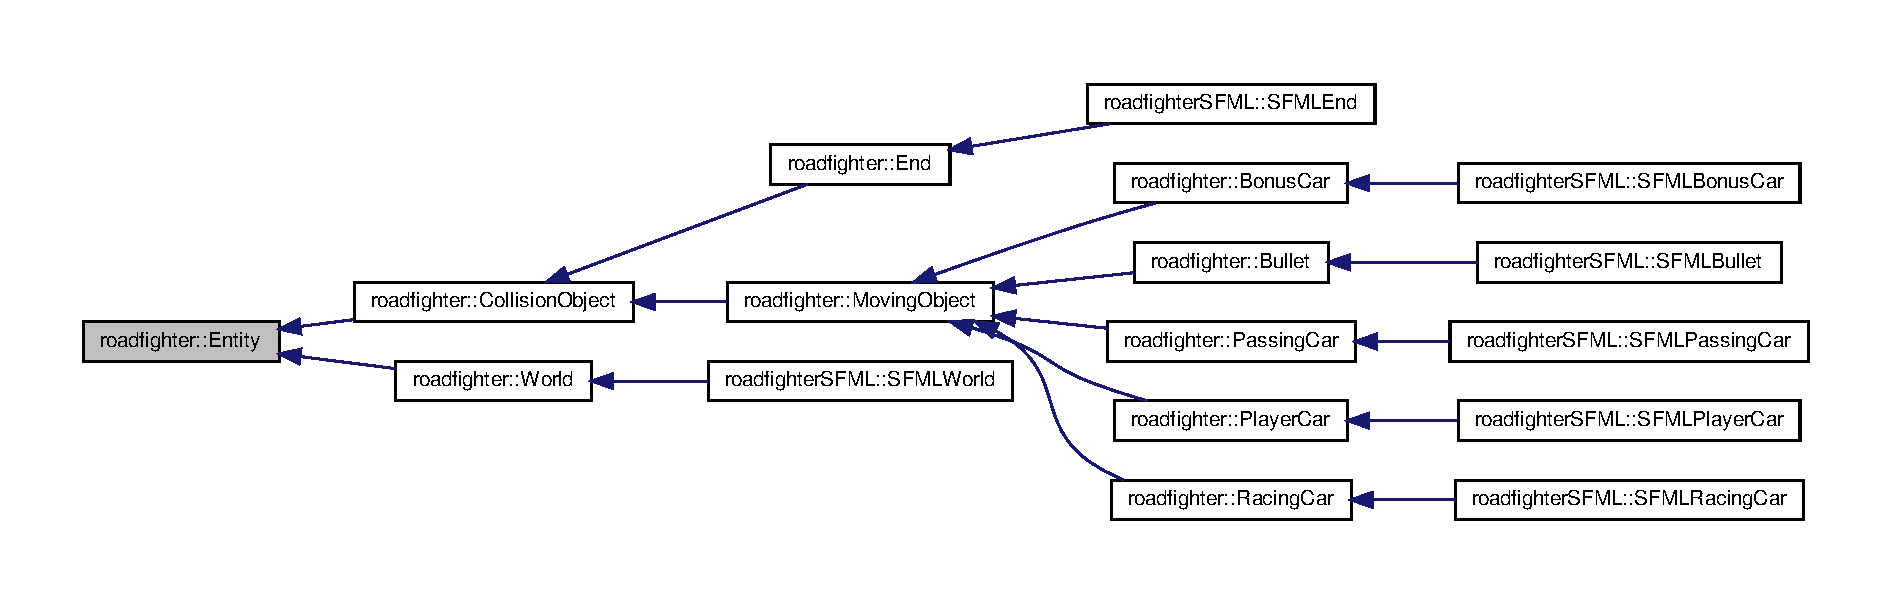
\includegraphics[width=350pt]{classroadfighter_1_1Entity__inherit__graph}
\end{center}
\end{figure}
\subsection*{Public Member Functions}
\begin{DoxyCompactItemize}
\item 
virtual void \hyperlink{classroadfighter_1_1Entity_a54c00f1af306290bae3e4b84e196566b}{update\+Logic} ()=0
\item 
virtual void \hyperlink{classroadfighter_1_1Entity_a66614a11004d6f9516473f60b530f689}{update\+Movement} (double dt)=0
\item 
virtual void \hyperlink{classroadfighter_1_1Entity_ac516f8005f969ad5a86c252e5a3640ee}{draw} ()=0
\end{DoxyCompactItemize}


\subsection{Member Function Documentation}
\mbox{\Hypertarget{classroadfighter_1_1Entity_ac516f8005f969ad5a86c252e5a3640ee}\label{classroadfighter_1_1Entity_ac516f8005f969ad5a86c252e5a3640ee}} 
\index{roadfighter\+::\+Entity@{roadfighter\+::\+Entity}!draw@{draw}}
\index{draw@{draw}!roadfighter\+::\+Entity@{roadfighter\+::\+Entity}}
\subsubsection{\texorpdfstring{draw()}{draw()}}
{\footnotesize\ttfamily virtual void roadfighter\+::\+Entity\+::draw (\begin{DoxyParamCaption}{ }\end{DoxyParamCaption})\hspace{0.3cm}{\ttfamily [pure virtual]}}

virtual void function that is used to draw the entity this function is not overriden in the game logic itself and should be implemented by the creator of the graphics implementation 

Implemented in \hyperlink{classroadfighter_1_1World_a90534263a154d6d7c1e8aef4e0138881}{roadfighter\+::\+World}, \hyperlink{classSFMLPlayerCar_ab4adedb2554e5f5eb59b7565a592c2b2}{S\+F\+M\+L\+Player\+Car}, \hyperlink{classSFMLBonusCar_a95d6a17fdbd099db1fe080da1581da20}{S\+F\+M\+L\+Bonus\+Car}, \hyperlink{classSFMLBullet_a2b774898d1f369ab6d1e58659dab389a}{S\+F\+M\+L\+Bullet}, \hyperlink{classSFMLPassingCar_ad860ff5f0eea98fffaa51381c9424e8d}{S\+F\+M\+L\+Passing\+Car}, \hyperlink{classSFMLRacingCar_a2b1c8b9ad2b80c9e18990cb078d2d62d}{S\+F\+M\+L\+Racing\+Car}, \hyperlink{classSFMLWorld_aa0e1deda989ca494937054c5f5b139b0}{S\+F\+M\+L\+World}, and \hyperlink{classSFMLEnd_aee51982a63f9c1c6495f539528683989}{S\+F\+M\+L\+End}.

\mbox{\Hypertarget{classroadfighter_1_1Entity_a54c00f1af306290bae3e4b84e196566b}\label{classroadfighter_1_1Entity_a54c00f1af306290bae3e4b84e196566b}} 
\index{roadfighter\+::\+Entity@{roadfighter\+::\+Entity}!update\+Logic@{update\+Logic}}
\index{update\+Logic@{update\+Logic}!roadfighter\+::\+Entity@{roadfighter\+::\+Entity}}
\subsubsection{\texorpdfstring{update\+Logic()}{updateLogic()}}
{\footnotesize\ttfamily virtual void roadfighter\+::\+Entity\+::update\+Logic (\begin{DoxyParamCaption}{ }\end{DoxyParamCaption})\hspace{0.3cm}{\ttfamily [pure virtual]}}

virtual void function that should be used to update the logic of the entity 

Implemented in \hyperlink{classroadfighter_1_1MovingObject_a2c5d69054a59fc5c6d7458f864ee9d57}{roadfighter\+::\+Moving\+Object}, \hyperlink{classroadfighter_1_1Bullet_a13aa730279ee8590d0eb2f9e6c01f265}{roadfighter\+::\+Bullet}, \hyperlink{classroadfighter_1_1PlayerCar_a01480487ca7978a50a3c6609f1ebe6df}{roadfighter\+::\+Player\+Car}, \hyperlink{classroadfighter_1_1World_a066592a75c8a38e241013707b429206c}{roadfighter\+::\+World}, \hyperlink{classroadfighter_1_1RacingCar_af3f3b4c368ba61c13dc9b99004895c5d}{roadfighter\+::\+Racing\+Car}, \hyperlink{classroadfighter_1_1BonusCar_a21d55ad1e1595ac6c86ca20f8819778b}{roadfighter\+::\+Bonus\+Car}, \hyperlink{classroadfighter_1_1PassingCar_ac3fe3087290121bf44880f94efa3a916}{roadfighter\+::\+Passing\+Car}, and \hyperlink{classroadfighter_1_1End_aee4a4fed3e7bd5f85f183351280e54f9}{roadfighter\+::\+End}.

\mbox{\Hypertarget{classroadfighter_1_1Entity_a66614a11004d6f9516473f60b530f689}\label{classroadfighter_1_1Entity_a66614a11004d6f9516473f60b530f689}} 
\index{roadfighter\+::\+Entity@{roadfighter\+::\+Entity}!update\+Movement@{update\+Movement}}
\index{update\+Movement@{update\+Movement}!roadfighter\+::\+Entity@{roadfighter\+::\+Entity}}
\subsubsection{\texorpdfstring{update\+Movement()}{updateMovement()}}
{\footnotesize\ttfamily virtual void roadfighter\+::\+Entity\+::update\+Movement (\begin{DoxyParamCaption}\item[{double}]{dt }\end{DoxyParamCaption})\hspace{0.3cm}{\ttfamily [pure virtual]}}

virtual void function that should be used to update the movement of the entity 
\begin{DoxyParams}{Parameters}
{\em dt} & \\
\hline
\end{DoxyParams}


Implemented in \hyperlink{classroadfighter_1_1MovingObject_ac1918d96dac118c4bd7d99168d92867c}{roadfighter\+::\+Moving\+Object}, \hyperlink{classroadfighter_1_1PlayerCar_aa1dcbec01dde1b212e4919b61338edde}{roadfighter\+::\+Player\+Car}, \hyperlink{classroadfighter_1_1World_a880776b589376b1b4fd5ed4f26de4482}{roadfighter\+::\+World}, \hyperlink{classroadfighter_1_1BonusCar_a2d3d584ca34a5df3b3c833123a9bbc30}{roadfighter\+::\+Bonus\+Car}, \hyperlink{classroadfighter_1_1PassingCar_ade5ebca5d7dbdb75bd9eee5817972363}{roadfighter\+::\+Passing\+Car}, \hyperlink{classroadfighter_1_1RacingCar_a2e8f3c63381a1fe432cddcc1f34fb935}{roadfighter\+::\+Racing\+Car}, and \hyperlink{classroadfighter_1_1End_a6ea4afe8b07f96801fb2a67b82d6b71c}{roadfighter\+::\+End}.



The documentation for this class was generated from the following file\+:\begin{DoxyCompactItemize}
\item 
Game\+Logic/include/\+Entities/Entity.\+h\end{DoxyCompactItemize}

\hypertarget{classroadfighter_1_1Entity__Factory__base}{}\section{roadfighter\+:\+:Entity\+\_\+\+Factory\+\_\+base Class Reference}
\label{classroadfighter_1_1Entity__Factory__base}\index{roadfighter\+::\+Entity\+\_\+\+Factory\+\_\+base@{roadfighter\+::\+Entity\+\_\+\+Factory\+\_\+base}}


Inheritance diagram for roadfighter\+:\+:Entity\+\_\+\+Factory\+\_\+base\+:
\nopagebreak
\begin{figure}[H]
\begin{center}
\leavevmode
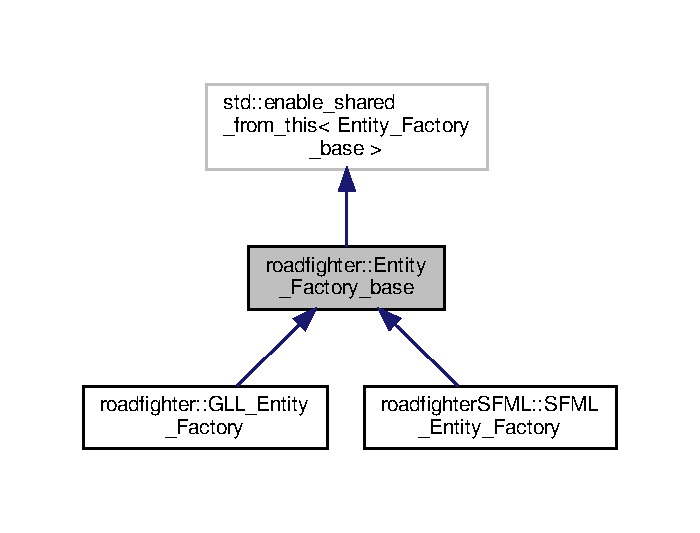
\includegraphics[width=336pt]{classroadfighter_1_1Entity__Factory__base__inherit__graph}
\end{center}
\end{figure}


Collaboration diagram for roadfighter\+:\+:Entity\+\_\+\+Factory\+\_\+base\+:\nopagebreak
\begin{figure}[H]
\begin{center}
\leavevmode
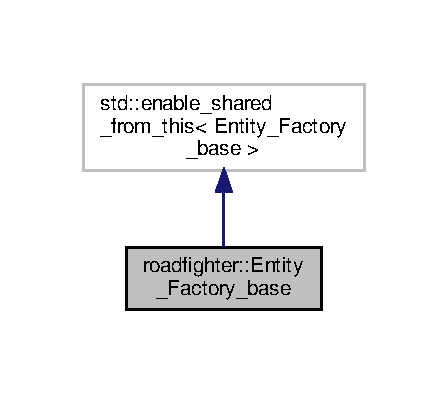
\includegraphics[width=215pt]{classroadfighter_1_1Entity__Factory__base__coll__graph}
\end{center}
\end{figure}
\subsection*{Public Member Functions}
\begin{DoxyCompactItemize}
\item 
virtual std\+::shared\+\_\+ptr$<$ \hyperlink{classroadfighter_1_1Entity}{Entity} $>$ \hyperlink{classroadfighter_1_1Entity__Factory__base_a5241bdb886a9f1b086d009a0f6478045}{create\+Bullet} (double x, double y, double v\+Speed)=0
\item 
virtual std\+::shared\+\_\+ptr$<$ \hyperlink{classroadfighter_1_1Entity}{Entity} $>$ \hyperlink{classroadfighter_1_1Entity__Factory__base_aa21b8cb23696844b7349ccf2c87d10fa}{creat\+Passing\+Car} (double x, double y, double v\+Speed)=0
\item 
virtual std\+::shared\+\_\+ptr$<$ \hyperlink{classroadfighter_1_1Entity}{Entity} $>$ \hyperlink{classroadfighter_1_1Entity__Factory__base_a3021f69b62b9df33706096381664d58f}{create\+Player\+Car} (double x, double y, double max, double v\+Accel, double h\+Accel, double fuel)=0
\item 
virtual std\+::shared\+\_\+ptr$<$ \hyperlink{classroadfighter_1_1Entity}{Entity} $>$ \hyperlink{classroadfighter_1_1Entity__Factory__base_a17b9c30501b8a11624bee8f1c24a6b7e}{create\+Racing\+Car} (double x, double y, double max, double v\+Accel, double h\+Accel)=0
\item 
virtual std\+::shared\+\_\+ptr$<$ \hyperlink{classroadfighter_1_1Entity}{Entity} $>$ \hyperlink{classroadfighter_1_1Entity__Factory__base_a888f537d2deed2d90a391c1900e9fdb6}{create\+Bonus\+Car} (double x, double y, double v\+Speed)=0
\item 
virtual std\+::shared\+\_\+ptr$<$ \hyperlink{classroadfighter_1_1Entity}{Entity} $>$ \hyperlink{classroadfighter_1_1Entity__Factory__base_a791574991ccbe7ff95f28e5651ed2cb1}{create\+End} (double y)=0
\item 
virtual std\+::shared\+\_\+ptr$<$ \hyperlink{classroadfighter_1_1Entity}{Entity} $>$ \hyperlink{classroadfighter_1_1Entity__Factory__base_aa24de6bbeb80c25e96f3e24d6bcb5169}{create\+World} ()=0
\item 
virtual \hyperlink{classroadfighter_1_1Entity__Factory__base_a19ec21ceb4fd132712ef1bf131b4be9b}{$\sim$\+Entity\+\_\+\+Factory\+\_\+base} ()=default
\item 
\hyperlink{classroadfighter_1_1Entity__Factory__base_a2c498f47c9cae7c34052b3b10e0cb3d2}{Entity\+\_\+\+Factory\+\_\+base} ()
\item 
void \hyperlink{classroadfighter_1_1Entity__Factory__base_a6c9363d763f34f39a44eaf02c6cb9f87}{set\+Controller} (const std\+::shared\+\_\+ptr$<$ \hyperlink{classroadfighter_1_1InputController}{Input\+Controller} $>$ \&m\+\_\+controller)
\item 
void \hyperlink{classroadfighter_1_1Entity__Factory__base_ab3338a586002c58ad7581e1046be9ba5}{set\+Transporter} (const std\+::shared\+\_\+ptr$<$ \hyperlink{classroadfighter_1_1EntityTransporter}{Entity\+Transporter} $>$ \&m\+\_\+\+Transporter)
\item 
const std\+::shared\+\_\+ptr$<$ \hyperlink{classroadfighter_1_1InputController}{Input\+Controller} $>$ \& \hyperlink{classroadfighter_1_1Entity__Factory__base_a3ea098a47127d87d64a6a8623035007a}{get\+Controller} () const
\item 
const std\+::shared\+\_\+ptr$<$ \hyperlink{classroadfighter_1_1EntityTransporter}{Entity\+Transporter} $>$ \& \hyperlink{classroadfighter_1_1Entity__Factory__base_a4a8d467738722cfb4f343de72a4a355a}{get\+Transporter} () const
\item 
const std\+::shared\+\_\+ptr$<$ \hyperlink{classroadfighter_1_1ObserverBase}{Observer\+Base} $>$ \& \hyperlink{classroadfighter_1_1Entity__Factory__base_a7b45161be0cda25b24375f6e99594bcc}{get\+Score\+Observer} () const
\item 
void \hyperlink{classroadfighter_1_1Entity__Factory__base_a59240ab3a76f6d54b051bc560b6d3aa1}{set\+Score\+Observer} (const std\+::shared\+\_\+ptr$<$ \hyperlink{classroadfighter_1_1ObserverBase}{Observer\+Base} $>$ \&m\+\_\+score\+Observer)
\end{DoxyCompactItemize}


\subsection{Constructor \& Destructor Documentation}
\mbox{\Hypertarget{classroadfighter_1_1Entity__Factory__base_a19ec21ceb4fd132712ef1bf131b4be9b}\label{classroadfighter_1_1Entity__Factory__base_a19ec21ceb4fd132712ef1bf131b4be9b}} 
\index{roadfighter\+::\+Entity\+\_\+\+Factory\+\_\+base@{roadfighter\+::\+Entity\+\_\+\+Factory\+\_\+base}!````~Entity\+\_\+\+Factory\+\_\+base@{$\sim$\+Entity\+\_\+\+Factory\+\_\+base}}
\index{````~Entity\+\_\+\+Factory\+\_\+base@{$\sim$\+Entity\+\_\+\+Factory\+\_\+base}!roadfighter\+::\+Entity\+\_\+\+Factory\+\_\+base@{roadfighter\+::\+Entity\+\_\+\+Factory\+\_\+base}}
\subsubsection{\texorpdfstring{$\sim$\+Entity\+\_\+\+Factory\+\_\+base()}{~Entity\_Factory\_base()}}
{\footnotesize\ttfamily virtual roadfighter\+::\+Entity\+\_\+\+Factory\+\_\+base\+::$\sim$\+Entity\+\_\+\+Factory\+\_\+base (\begin{DoxyParamCaption}{ }\end{DoxyParamCaption})\hspace{0.3cm}{\ttfamily [virtual]}, {\ttfamily [default]}}

virtual destructor \mbox{\Hypertarget{classroadfighter_1_1Entity__Factory__base_a2c498f47c9cae7c34052b3b10e0cb3d2}\label{classroadfighter_1_1Entity__Factory__base_a2c498f47c9cae7c34052b3b10e0cb3d2}} 
\index{roadfighter\+::\+Entity\+\_\+\+Factory\+\_\+base@{roadfighter\+::\+Entity\+\_\+\+Factory\+\_\+base}!Entity\+\_\+\+Factory\+\_\+base@{Entity\+\_\+\+Factory\+\_\+base}}
\index{Entity\+\_\+\+Factory\+\_\+base@{Entity\+\_\+\+Factory\+\_\+base}!roadfighter\+::\+Entity\+\_\+\+Factory\+\_\+base@{roadfighter\+::\+Entity\+\_\+\+Factory\+\_\+base}}
\subsubsection{\texorpdfstring{Entity\+\_\+\+Factory\+\_\+base()}{Entity\_Factory\_base()}}
{\footnotesize\ttfamily roadfighter\+::\+Entity\+\_\+\+Factory\+\_\+base\+::\+Entity\+\_\+\+Factory\+\_\+base (\begin{DoxyParamCaption}{ }\end{DoxyParamCaption})}

constructor for base entity factory \begin{DoxyReturn}{Returns}
none 
\end{DoxyReturn}

\begin{DoxyExceptions}{Exceptions}
{\em none} & \\
\hline
\end{DoxyExceptions}


\subsection{Member Function Documentation}
\mbox{\Hypertarget{classroadfighter_1_1Entity__Factory__base_a888f537d2deed2d90a391c1900e9fdb6}\label{classroadfighter_1_1Entity__Factory__base_a888f537d2deed2d90a391c1900e9fdb6}} 
\index{roadfighter\+::\+Entity\+\_\+\+Factory\+\_\+base@{roadfighter\+::\+Entity\+\_\+\+Factory\+\_\+base}!create\+Bonus\+Car@{create\+Bonus\+Car}}
\index{create\+Bonus\+Car@{create\+Bonus\+Car}!roadfighter\+::\+Entity\+\_\+\+Factory\+\_\+base@{roadfighter\+::\+Entity\+\_\+\+Factory\+\_\+base}}
\subsubsection{\texorpdfstring{create\+Bonus\+Car()}{createBonusCar()}}
{\footnotesize\ttfamily virtual std\+::shared\+\_\+ptr$<$\hyperlink{classroadfighter_1_1Entity}{Entity}$>$ roadfighter\+::\+Entity\+\_\+\+Factory\+\_\+base\+::create\+Bonus\+Car (\begin{DoxyParamCaption}\item[{double}]{x,  }\item[{double}]{y,  }\item[{double}]{v\+Speed }\end{DoxyParamCaption})\hspace{0.3cm}{\ttfamily [pure virtual]}}

base factory method for creating a \hyperlink{classroadfighter_1_1BonusCar}{Bonus\+Car} 
\begin{DoxyParams}{Parameters}
{\em x} & coordinate of the bonus car (the middle) \\
\hline
{\em y} & coordinate of the passing bonus car (the middle) \\
\hline
{\em v\+Speed} & the set speed of the passingcar \\
\hline
\end{DoxyParams}
\begin{DoxyReturn}{Returns}
a shared pointer to an entity 
\end{DoxyReturn}


Implemented in \hyperlink{classroadfighterSFML_1_1SFML__Entity__Factory_a61a1a52caf4c051ce0880eb19ae028eb}{roadfighter\+S\+F\+M\+L\+::\+S\+F\+M\+L\+\_\+\+Entity\+\_\+\+Factory}, and \hyperlink{classroadfighter_1_1GLL__Entity__Factory_a2a6a8d397d43c48894adb6c9d9ed0947}{roadfighter\+::\+G\+L\+L\+\_\+\+Entity\+\_\+\+Factory}.

\mbox{\Hypertarget{classroadfighter_1_1Entity__Factory__base_a5241bdb886a9f1b086d009a0f6478045}\label{classroadfighter_1_1Entity__Factory__base_a5241bdb886a9f1b086d009a0f6478045}} 
\index{roadfighter\+::\+Entity\+\_\+\+Factory\+\_\+base@{roadfighter\+::\+Entity\+\_\+\+Factory\+\_\+base}!create\+Bullet@{create\+Bullet}}
\index{create\+Bullet@{create\+Bullet}!roadfighter\+::\+Entity\+\_\+\+Factory\+\_\+base@{roadfighter\+::\+Entity\+\_\+\+Factory\+\_\+base}}
\subsubsection{\texorpdfstring{create\+Bullet()}{createBullet()}}
{\footnotesize\ttfamily virtual std\+::shared\+\_\+ptr$<$\hyperlink{classroadfighter_1_1Entity}{Entity}$>$ roadfighter\+::\+Entity\+\_\+\+Factory\+\_\+base\+::create\+Bullet (\begin{DoxyParamCaption}\item[{double}]{x,  }\item[{double}]{y,  }\item[{double}]{v\+Speed }\end{DoxyParamCaption})\hspace{0.3cm}{\ttfamily [pure virtual]}}

base factory method for creating a bullet \begin{DoxyReturn}{Returns}
a shared pointer to an \hyperlink{classroadfighter_1_1Entity}{Entity} 
\end{DoxyReturn}


Implemented in \hyperlink{classroadfighterSFML_1_1SFML__Entity__Factory_aa8da7f42177db63a837596100c21dc88}{roadfighter\+S\+F\+M\+L\+::\+S\+F\+M\+L\+\_\+\+Entity\+\_\+\+Factory}, and \hyperlink{classroadfighter_1_1GLL__Entity__Factory_a7fcd57b8a2ae18240476f6dc64216822}{roadfighter\+::\+G\+L\+L\+\_\+\+Entity\+\_\+\+Factory}.

\mbox{\Hypertarget{classroadfighter_1_1Entity__Factory__base_a791574991ccbe7ff95f28e5651ed2cb1}\label{classroadfighter_1_1Entity__Factory__base_a791574991ccbe7ff95f28e5651ed2cb1}} 
\index{roadfighter\+::\+Entity\+\_\+\+Factory\+\_\+base@{roadfighter\+::\+Entity\+\_\+\+Factory\+\_\+base}!create\+End@{create\+End}}
\index{create\+End@{create\+End}!roadfighter\+::\+Entity\+\_\+\+Factory\+\_\+base@{roadfighter\+::\+Entity\+\_\+\+Factory\+\_\+base}}
\subsubsection{\texorpdfstring{create\+End()}{createEnd()}}
{\footnotesize\ttfamily virtual std\+::shared\+\_\+ptr$<$\hyperlink{classroadfighter_1_1Entity}{Entity}$>$ roadfighter\+::\+Entity\+\_\+\+Factory\+\_\+base\+::create\+End (\begin{DoxyParamCaption}\item[{double}]{y }\end{DoxyParamCaption})\hspace{0.3cm}{\ttfamily [pure virtual]}}

base factory method for creating a \hyperlink{classroadfighter_1_1End}{End} 
\begin{DoxyParams}{Parameters}
{\em y} & coordinate of the end \\
\hline
\end{DoxyParams}
\begin{DoxyReturn}{Returns}
a shared pointer to an entity 
\end{DoxyReturn}


Implemented in \hyperlink{classroadfighterSFML_1_1SFML__Entity__Factory_ac7136d6a99235606f220508719535e08}{roadfighter\+S\+F\+M\+L\+::\+S\+F\+M\+L\+\_\+\+Entity\+\_\+\+Factory}, and \hyperlink{classroadfighter_1_1GLL__Entity__Factory_ae26222829d8295cef0aa708a7ee909b7}{roadfighter\+::\+G\+L\+L\+\_\+\+Entity\+\_\+\+Factory}.

\mbox{\Hypertarget{classroadfighter_1_1Entity__Factory__base_a3021f69b62b9df33706096381664d58f}\label{classroadfighter_1_1Entity__Factory__base_a3021f69b62b9df33706096381664d58f}} 
\index{roadfighter\+::\+Entity\+\_\+\+Factory\+\_\+base@{roadfighter\+::\+Entity\+\_\+\+Factory\+\_\+base}!create\+Player\+Car@{create\+Player\+Car}}
\index{create\+Player\+Car@{create\+Player\+Car}!roadfighter\+::\+Entity\+\_\+\+Factory\+\_\+base@{roadfighter\+::\+Entity\+\_\+\+Factory\+\_\+base}}
\subsubsection{\texorpdfstring{create\+Player\+Car()}{createPlayerCar()}}
{\footnotesize\ttfamily virtual std\+::shared\+\_\+ptr$<$\hyperlink{classroadfighter_1_1Entity}{Entity}$>$ roadfighter\+::\+Entity\+\_\+\+Factory\+\_\+base\+::create\+Player\+Car (\begin{DoxyParamCaption}\item[{double}]{x,  }\item[{double}]{y,  }\item[{double}]{max,  }\item[{double}]{v\+Accel,  }\item[{double}]{h\+Accel,  }\item[{double}]{fuel }\end{DoxyParamCaption})\hspace{0.3cm}{\ttfamily [pure virtual]}}

base factory method for crating the player car 
\begin{DoxyParams}{Parameters}
{\em x} & xcoordinate of the player car (the middle) \\
\hline
{\em y} & coordinate of the player car (the middle) \\
\hline
{\em max} & the max vertical speed \\
\hline
{\em v\+Accel} & the vertical acceleration per tick \\
\hline
{\em h\+Accel} & the horizontal acceleration per tick \\
\hline
{\em fuel} & the starting fuel of the car \\
\hline
\end{DoxyParams}
\begin{DoxyReturn}{Returns}
a shared pointer to an entity 
\end{DoxyReturn}


Implemented in \hyperlink{classroadfighterSFML_1_1SFML__Entity__Factory_a3ac3b1c7e0f692fbf37b7bdbe6738806}{roadfighter\+S\+F\+M\+L\+::\+S\+F\+M\+L\+\_\+\+Entity\+\_\+\+Factory}, and \hyperlink{classroadfighter_1_1GLL__Entity__Factory_a45992523d105bd284b7aeed6cb41ce8a}{roadfighter\+::\+G\+L\+L\+\_\+\+Entity\+\_\+\+Factory}.

\mbox{\Hypertarget{classroadfighter_1_1Entity__Factory__base_a17b9c30501b8a11624bee8f1c24a6b7e}\label{classroadfighter_1_1Entity__Factory__base_a17b9c30501b8a11624bee8f1c24a6b7e}} 
\index{roadfighter\+::\+Entity\+\_\+\+Factory\+\_\+base@{roadfighter\+::\+Entity\+\_\+\+Factory\+\_\+base}!create\+Racing\+Car@{create\+Racing\+Car}}
\index{create\+Racing\+Car@{create\+Racing\+Car}!roadfighter\+::\+Entity\+\_\+\+Factory\+\_\+base@{roadfighter\+::\+Entity\+\_\+\+Factory\+\_\+base}}
\subsubsection{\texorpdfstring{create\+Racing\+Car()}{createRacingCar()}}
{\footnotesize\ttfamily virtual std\+::shared\+\_\+ptr$<$\hyperlink{classroadfighter_1_1Entity}{Entity}$>$ roadfighter\+::\+Entity\+\_\+\+Factory\+\_\+base\+::create\+Racing\+Car (\begin{DoxyParamCaption}\item[{double}]{x,  }\item[{double}]{y,  }\item[{double}]{max,  }\item[{double}]{v\+Accel,  }\item[{double}]{h\+Accel }\end{DoxyParamCaption})\hspace{0.3cm}{\ttfamily [pure virtual]}}

base factory method for crating a racing car 
\begin{DoxyParams}{Parameters}
{\em x} & xcoordinate of the racing car (the middle) \\
\hline
{\em y} & coordinate of the racing car (the middle) \\
\hline
{\em max} & the max vertical speed \\
\hline
{\em v\+Accel} & the vertical acceleration per tick \\
\hline
{\em h\+Accel} & the horizontal acceleration per tick \\
\hline
\end{DoxyParams}
\begin{DoxyReturn}{Returns}
a shared pointer to an entity 
\end{DoxyReturn}


Implemented in \hyperlink{classroadfighterSFML_1_1SFML__Entity__Factory_a0002a898c840c69f86bf2756ffa27703}{roadfighter\+S\+F\+M\+L\+::\+S\+F\+M\+L\+\_\+\+Entity\+\_\+\+Factory}, and \hyperlink{classroadfighter_1_1GLL__Entity__Factory_a81737f6acc8d3c460b4d244cf06baeec}{roadfighter\+::\+G\+L\+L\+\_\+\+Entity\+\_\+\+Factory}.

\mbox{\Hypertarget{classroadfighter_1_1Entity__Factory__base_aa24de6bbeb80c25e96f3e24d6bcb5169}\label{classroadfighter_1_1Entity__Factory__base_aa24de6bbeb80c25e96f3e24d6bcb5169}} 
\index{roadfighter\+::\+Entity\+\_\+\+Factory\+\_\+base@{roadfighter\+::\+Entity\+\_\+\+Factory\+\_\+base}!create\+World@{create\+World}}
\index{create\+World@{create\+World}!roadfighter\+::\+Entity\+\_\+\+Factory\+\_\+base@{roadfighter\+::\+Entity\+\_\+\+Factory\+\_\+base}}
\subsubsection{\texorpdfstring{create\+World()}{createWorld()}}
{\footnotesize\ttfamily virtual std\+::shared\+\_\+ptr$<$\hyperlink{classroadfighter_1_1Entity}{Entity}$>$ roadfighter\+::\+Entity\+\_\+\+Factory\+\_\+base\+::create\+World (\begin{DoxyParamCaption}{ }\end{DoxyParamCaption})\hspace{0.3cm}{\ttfamily [pure virtual]}}

base factory method for creating the world \begin{DoxyReturn}{Returns}
a shared pointer to an entity 
\end{DoxyReturn}


Implemented in \hyperlink{classroadfighterSFML_1_1SFML__Entity__Factory_a163d8547144ca9509721d2a3aef0fa89}{roadfighter\+S\+F\+M\+L\+::\+S\+F\+M\+L\+\_\+\+Entity\+\_\+\+Factory}, and \hyperlink{classroadfighter_1_1GLL__Entity__Factory_a80f9f647f1192ddc098b2aa4f0172168}{roadfighter\+::\+G\+L\+L\+\_\+\+Entity\+\_\+\+Factory}.

\mbox{\Hypertarget{classroadfighter_1_1Entity__Factory__base_aa21b8cb23696844b7349ccf2c87d10fa}\label{classroadfighter_1_1Entity__Factory__base_aa21b8cb23696844b7349ccf2c87d10fa}} 
\index{roadfighter\+::\+Entity\+\_\+\+Factory\+\_\+base@{roadfighter\+::\+Entity\+\_\+\+Factory\+\_\+base}!creat\+Passing\+Car@{creat\+Passing\+Car}}
\index{creat\+Passing\+Car@{creat\+Passing\+Car}!roadfighter\+::\+Entity\+\_\+\+Factory\+\_\+base@{roadfighter\+::\+Entity\+\_\+\+Factory\+\_\+base}}
\subsubsection{\texorpdfstring{creat\+Passing\+Car()}{creatPassingCar()}}
{\footnotesize\ttfamily virtual std\+::shared\+\_\+ptr$<$\hyperlink{classroadfighter_1_1Entity}{Entity}$>$ roadfighter\+::\+Entity\+\_\+\+Factory\+\_\+base\+::creat\+Passing\+Car (\begin{DoxyParamCaption}\item[{double}]{x,  }\item[{double}]{y,  }\item[{double}]{v\+Speed }\end{DoxyParamCaption})\hspace{0.3cm}{\ttfamily [pure virtual]}}

base factory method for creating a \hyperlink{classroadfighter_1_1PassingCar}{Passing\+Car} 
\begin{DoxyParams}{Parameters}
{\em x} & coordinate of the passing car (the middle) \\
\hline
{\em y} & coordinate of the passing car (the middle) \\
\hline
{\em v\+Speed} & the set speed of the passingcar \\
\hline
\end{DoxyParams}
\begin{DoxyReturn}{Returns}
a shared pointer to an entity 
\end{DoxyReturn}


Implemented in \hyperlink{classroadfighterSFML_1_1SFML__Entity__Factory_a3944854c727ab2c6c5007acff997c0b4}{roadfighter\+S\+F\+M\+L\+::\+S\+F\+M\+L\+\_\+\+Entity\+\_\+\+Factory}, and \hyperlink{classroadfighter_1_1GLL__Entity__Factory_aa176b2bec6007989c5cf3658840123c7}{roadfighter\+::\+G\+L\+L\+\_\+\+Entity\+\_\+\+Factory}.

\mbox{\Hypertarget{classroadfighter_1_1Entity__Factory__base_a3ea098a47127d87d64a6a8623035007a}\label{classroadfighter_1_1Entity__Factory__base_a3ea098a47127d87d64a6a8623035007a}} 
\index{roadfighter\+::\+Entity\+\_\+\+Factory\+\_\+base@{roadfighter\+::\+Entity\+\_\+\+Factory\+\_\+base}!get\+Controller@{get\+Controller}}
\index{get\+Controller@{get\+Controller}!roadfighter\+::\+Entity\+\_\+\+Factory\+\_\+base@{roadfighter\+::\+Entity\+\_\+\+Factory\+\_\+base}}
\subsubsection{\texorpdfstring{get\+Controller()}{getController()}}
{\footnotesize\ttfamily const std\+::shared\+\_\+ptr$<$ \hyperlink{classroadfighter_1_1InputController}{Input\+Controller} $>$ \& roadfighter\+::\+Entity\+\_\+\+Factory\+\_\+base\+::get\+Controller (\begin{DoxyParamCaption}{ }\end{DoxyParamCaption}) const}

getter for the controller \begin{DoxyReturn}{Returns}
a shared pointer to the movecontroller 
\end{DoxyReturn}
\mbox{\Hypertarget{classroadfighter_1_1Entity__Factory__base_a7b45161be0cda25b24375f6e99594bcc}\label{classroadfighter_1_1Entity__Factory__base_a7b45161be0cda25b24375f6e99594bcc}} 
\index{roadfighter\+::\+Entity\+\_\+\+Factory\+\_\+base@{roadfighter\+::\+Entity\+\_\+\+Factory\+\_\+base}!get\+Score\+Observer@{get\+Score\+Observer}}
\index{get\+Score\+Observer@{get\+Score\+Observer}!roadfighter\+::\+Entity\+\_\+\+Factory\+\_\+base@{roadfighter\+::\+Entity\+\_\+\+Factory\+\_\+base}}
\subsubsection{\texorpdfstring{get\+Score\+Observer()}{getScoreObserver()}}
{\footnotesize\ttfamily const std\+::shared\+\_\+ptr$<$ \hyperlink{classroadfighter_1_1ObserverBase}{Observer\+Base} $>$ \& roadfighter\+::\+Entity\+\_\+\+Factory\+\_\+base\+::get\+Score\+Observer (\begin{DoxyParamCaption}{ }\end{DoxyParamCaption}) const}

getter for the scoreobserver \begin{DoxyReturn}{Returns}
reference to std\+::shared\+\_\+ptr$<$\+Observer\+Base$>$ 
\end{DoxyReturn}

\begin{DoxyExceptions}{Exceptions}
{\em none} & \\
\hline
\end{DoxyExceptions}
\mbox{\Hypertarget{classroadfighter_1_1Entity__Factory__base_a4a8d467738722cfb4f343de72a4a355a}\label{classroadfighter_1_1Entity__Factory__base_a4a8d467738722cfb4f343de72a4a355a}} 
\index{roadfighter\+::\+Entity\+\_\+\+Factory\+\_\+base@{roadfighter\+::\+Entity\+\_\+\+Factory\+\_\+base}!get\+Transporter@{get\+Transporter}}
\index{get\+Transporter@{get\+Transporter}!roadfighter\+::\+Entity\+\_\+\+Factory\+\_\+base@{roadfighter\+::\+Entity\+\_\+\+Factory\+\_\+base}}
\subsubsection{\texorpdfstring{get\+Transporter()}{getTransporter()}}
{\footnotesize\ttfamily const std\+::shared\+\_\+ptr$<$ \hyperlink{classroadfighter_1_1EntityTransporter}{Entity\+Transporter} $>$ \& roadfighter\+::\+Entity\+\_\+\+Factory\+\_\+base\+::get\+Transporter (\begin{DoxyParamCaption}{ }\end{DoxyParamCaption}) const}

getter for the transporter \begin{DoxyReturn}{Returns}
a shared pointer to the entitytransporter 
\end{DoxyReturn}

\begin{DoxyExceptions}{Exceptions}
{\em none} & \\
\hline
\end{DoxyExceptions}
\mbox{\Hypertarget{classroadfighter_1_1Entity__Factory__base_a6c9363d763f34f39a44eaf02c6cb9f87}\label{classroadfighter_1_1Entity__Factory__base_a6c9363d763f34f39a44eaf02c6cb9f87}} 
\index{roadfighter\+::\+Entity\+\_\+\+Factory\+\_\+base@{roadfighter\+::\+Entity\+\_\+\+Factory\+\_\+base}!set\+Controller@{set\+Controller}}
\index{set\+Controller@{set\+Controller}!roadfighter\+::\+Entity\+\_\+\+Factory\+\_\+base@{roadfighter\+::\+Entity\+\_\+\+Factory\+\_\+base}}
\subsubsection{\texorpdfstring{set\+Controller()}{setController()}}
{\footnotesize\ttfamily void roadfighter\+::\+Entity\+\_\+\+Factory\+\_\+base\+::set\+Controller (\begin{DoxyParamCaption}\item[{const std\+::shared\+\_\+ptr$<$ \hyperlink{classroadfighter_1_1InputController}{Input\+Controller} $>$ \&}]{m\+\_\+controller }\end{DoxyParamCaption})}

sets the controller of the factory 
\begin{DoxyParams}{Parameters}
{\em m\+\_\+controller} & a movecontroller that will be given to all playercars created with this factory \\
\hline
\end{DoxyParams}
\mbox{\Hypertarget{classroadfighter_1_1Entity__Factory__base_a59240ab3a76f6d54b051bc560b6d3aa1}\label{classroadfighter_1_1Entity__Factory__base_a59240ab3a76f6d54b051bc560b6d3aa1}} 
\index{roadfighter\+::\+Entity\+\_\+\+Factory\+\_\+base@{roadfighter\+::\+Entity\+\_\+\+Factory\+\_\+base}!set\+Score\+Observer@{set\+Score\+Observer}}
\index{set\+Score\+Observer@{set\+Score\+Observer}!roadfighter\+::\+Entity\+\_\+\+Factory\+\_\+base@{roadfighter\+::\+Entity\+\_\+\+Factory\+\_\+base}}
\subsubsection{\texorpdfstring{set\+Score\+Observer()}{setScoreObserver()}}
{\footnotesize\ttfamily void roadfighter\+::\+Entity\+\_\+\+Factory\+\_\+base\+::set\+Score\+Observer (\begin{DoxyParamCaption}\item[{const std\+::shared\+\_\+ptr$<$ \hyperlink{classroadfighter_1_1ObserverBase}{Observer\+Base} $>$ \&}]{m\+\_\+score\+Observer }\end{DoxyParamCaption})}

setter for the score observer 
\begin{DoxyParams}{Parameters}
{\em m\+\_\+score\+Observer} & the new scoreobserver \\
\hline
\end{DoxyParams}
\begin{DoxyReturn}{Returns}
none 
\end{DoxyReturn}

\begin{DoxyExceptions}{Exceptions}
{\em none} & \\
\hline
\end{DoxyExceptions}
\mbox{\Hypertarget{classroadfighter_1_1Entity__Factory__base_ab3338a586002c58ad7581e1046be9ba5}\label{classroadfighter_1_1Entity__Factory__base_ab3338a586002c58ad7581e1046be9ba5}} 
\index{roadfighter\+::\+Entity\+\_\+\+Factory\+\_\+base@{roadfighter\+::\+Entity\+\_\+\+Factory\+\_\+base}!set\+Transporter@{set\+Transporter}}
\index{set\+Transporter@{set\+Transporter}!roadfighter\+::\+Entity\+\_\+\+Factory\+\_\+base@{roadfighter\+::\+Entity\+\_\+\+Factory\+\_\+base}}
\subsubsection{\texorpdfstring{set\+Transporter()}{setTransporter()}}
{\footnotesize\ttfamily void roadfighter\+::\+Entity\+\_\+\+Factory\+\_\+base\+::set\+Transporter (\begin{DoxyParamCaption}\item[{const std\+::shared\+\_\+ptr$<$ \hyperlink{classroadfighter_1_1EntityTransporter}{Entity\+Transporter} $>$ \&}]{m\+\_\+\+Transporter }\end{DoxyParamCaption})}

setter for the transporter 
\begin{DoxyParams}{Parameters}
{\em m\+\_\+\+Transporter} & an entitytransporter that will be given to the world \\
\hline
\end{DoxyParams}


The documentation for this class was generated from the following files\+:\begin{DoxyCompactItemize}
\item 
Game\+Logic/include/\hyperlink{Entity__Factory__base_8h}{Entity\+\_\+\+Factory\+\_\+base.\+h}\item 
Game\+Logic/\+Source/\hyperlink{Entity__Factory__base_8cpp}{Entity\+\_\+\+Factory\+\_\+base.\+cpp}\end{DoxyCompactItemize}

\hypertarget{classroadfighter_1_1EntityTransporter}{}\section{roadfighter\+:\+:Entity\+Transporter Class Reference}
\label{classroadfighter_1_1EntityTransporter}\index{roadfighter\+::\+Entity\+Transporter@{roadfighter\+::\+Entity\+Transporter}}
\subsection*{Public Member Functions}
\begin{DoxyCompactItemize}
\item 
void \hyperlink{classroadfighter_1_1EntityTransporter_ac5f01c9a0b33b25f29864bd00acf0611}{add\+Entity} (std\+::shared\+\_\+ptr$<$ \hyperlink{classroadfighter_1_1Entity}{Entity} $>$ to\+Add)
\item 
std\+::vector$<$ std\+::shared\+\_\+ptr$<$ \hyperlink{classroadfighter_1_1Entity}{Entity} $>$ $>$ \& \hyperlink{classroadfighter_1_1EntityTransporter_ac19204b4b7104561957b3a741fd6ceb5}{get\+Entities} ()
\item 
void \hyperlink{classroadfighter_1_1EntityTransporter_ac0e443566db9213272103952eb697d92}{clear} ()
\end{DoxyCompactItemize}


\subsection{Member Function Documentation}
\mbox{\Hypertarget{classroadfighter_1_1EntityTransporter_ac5f01c9a0b33b25f29864bd00acf0611}\label{classroadfighter_1_1EntityTransporter_ac5f01c9a0b33b25f29864bd00acf0611}} 
\index{roadfighter\+::\+Entity\+Transporter@{roadfighter\+::\+Entity\+Transporter}!add\+Entity@{add\+Entity}}
\index{add\+Entity@{add\+Entity}!roadfighter\+::\+Entity\+Transporter@{roadfighter\+::\+Entity\+Transporter}}
\subsubsection{\texorpdfstring{add\+Entity()}{addEntity()}}
{\footnotesize\ttfamily void roadfighter\+::\+Entity\+Transporter\+::add\+Entity (\begin{DoxyParamCaption}\item[{std\+::shared\+\_\+ptr$<$ \hyperlink{classroadfighter_1_1Entity}{Entity} $>$}]{to\+Add }\end{DoxyParamCaption})}

add an entity to the transporter 
\begin{DoxyParams}{Parameters}
{\em to\+Add} & a shared pointer to an entity \\
\hline
\end{DoxyParams}
\begin{DoxyReturn}{Returns}
none 
\end{DoxyReturn}

\begin{DoxyExceptions}{Exceptions}
{\em none} & \\
\hline
\end{DoxyExceptions}
\mbox{\Hypertarget{classroadfighter_1_1EntityTransporter_ac0e443566db9213272103952eb697d92}\label{classroadfighter_1_1EntityTransporter_ac0e443566db9213272103952eb697d92}} 
\index{roadfighter\+::\+Entity\+Transporter@{roadfighter\+::\+Entity\+Transporter}!clear@{clear}}
\index{clear@{clear}!roadfighter\+::\+Entity\+Transporter@{roadfighter\+::\+Entity\+Transporter}}
\subsubsection{\texorpdfstring{clear()}{clear()}}
{\footnotesize\ttfamily void roadfighter\+::\+Entity\+Transporter\+::clear (\begin{DoxyParamCaption}{ }\end{DoxyParamCaption})}

removes all the entities that are currently in the vector \begin{DoxyReturn}{Returns}
none 
\end{DoxyReturn}

\begin{DoxyExceptions}{Exceptions}
{\em none} & \\
\hline
\end{DoxyExceptions}
\mbox{\Hypertarget{classroadfighter_1_1EntityTransporter_ac19204b4b7104561957b3a741fd6ceb5}\label{classroadfighter_1_1EntityTransporter_ac19204b4b7104561957b3a741fd6ceb5}} 
\index{roadfighter\+::\+Entity\+Transporter@{roadfighter\+::\+Entity\+Transporter}!get\+Entities@{get\+Entities}}
\index{get\+Entities@{get\+Entities}!roadfighter\+::\+Entity\+Transporter@{roadfighter\+::\+Entity\+Transporter}}
\subsubsection{\texorpdfstring{get\+Entities()}{getEntities()}}
{\footnotesize\ttfamily std\+::vector$<$ std\+::shared\+\_\+ptr$<$ \hyperlink{classroadfighter_1_1Entity}{roadfighter\+::\+Entity} $>$ $>$ \& roadfighter\+::\+Entity\+Transporter\+::get\+Entities (\begin{DoxyParamCaption}{ }\end{DoxyParamCaption})}

gets all the entities currently in the transporter \begin{DoxyReturn}{Returns}
a vector of shard pointers to entities 
\end{DoxyReturn}

\begin{DoxyExceptions}{Exceptions}
{\em none} & \\
\hline
\end{DoxyExceptions}


The documentation for this class was generated from the following files\+:\begin{DoxyCompactItemize}
\item 
Game\+Logic/include/\hyperlink{EntityTransporter_8h}{Entity\+Transporter.\+h}\item 
Game\+Logic/\+Source/\hyperlink{EntityTransporter_8cpp}{Entity\+Transporter.\+cpp}\end{DoxyCompactItemize}

\hypertarget{classroadfighter_1_1GLL__Entity__Factory}{}\section{roadfighter\+:\+:G\+L\+L\+\_\+\+Entity\+\_\+\+Factory Class Reference}
\label{classroadfighter_1_1GLL__Entity__Factory}\index{roadfighter\+::\+G\+L\+L\+\_\+\+Entity\+\_\+\+Factory@{roadfighter\+::\+G\+L\+L\+\_\+\+Entity\+\_\+\+Factory}}


Inheritance diagram for roadfighter\+:\+:G\+L\+L\+\_\+\+Entity\+\_\+\+Factory\+:\nopagebreak
\begin{figure}[H]
\begin{center}
\leavevmode
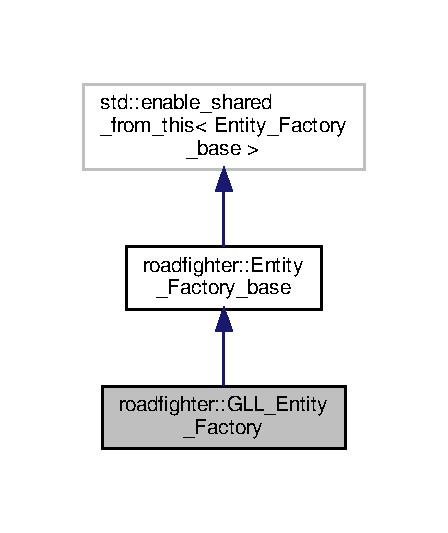
\includegraphics[width=215pt]{classroadfighter_1_1GLL__Entity__Factory__inherit__graph}
\end{center}
\end{figure}


Collaboration diagram for roadfighter\+:\+:G\+L\+L\+\_\+\+Entity\+\_\+\+Factory\+:\nopagebreak
\begin{figure}[H]
\begin{center}
\leavevmode
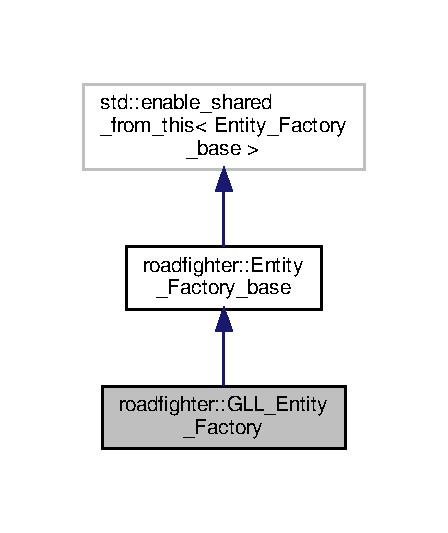
\includegraphics[width=215pt]{classroadfighter_1_1GLL__Entity__Factory__coll__graph}
\end{center}
\end{figure}
\subsection*{Public Member Functions}
\begin{DoxyCompactItemize}
\item 
\hyperlink{classroadfighter_1_1GLL__Entity__Factory_ab9689b5c0b2eae42b1b5e3dc1dcc46e0}{G\+L\+L\+\_\+\+Entity\+\_\+\+Factory} ()=default
\item 
std\+::shared\+\_\+ptr$<$ \hyperlink{classroadfighter_1_1Entity}{Entity} $>$ \hyperlink{classroadfighter_1_1GLL__Entity__Factory_a7fcd57b8a2ae18240476f6dc64216822}{create\+Bullet} (double x, double y, double v\+Speed) override
\item 
std\+::shared\+\_\+ptr$<$ \hyperlink{classroadfighter_1_1Entity}{Entity} $>$ \hyperlink{classroadfighter_1_1GLL__Entity__Factory_aa176b2bec6007989c5cf3658840123c7}{creat\+Passing\+Car} (double x, double y, double v\+Speed) override
\item 
std\+::shared\+\_\+ptr$<$ \hyperlink{classroadfighter_1_1Entity}{Entity} $>$ \hyperlink{classroadfighter_1_1GLL__Entity__Factory_a45992523d105bd284b7aeed6cb41ce8a}{create\+Player\+Car} (double x, double y, double max, double v\+Accel, double h\+Accel, double fuel) override
\item 
std\+::shared\+\_\+ptr$<$ \hyperlink{classroadfighter_1_1Entity}{Entity} $>$ \hyperlink{classroadfighter_1_1GLL__Entity__Factory_a81737f6acc8d3c460b4d244cf06baeec}{create\+Racing\+Car} (double x, double y, double max, double v\+Accel, double h\+Accel) override
\item 
std\+::shared\+\_\+ptr$<$ \hyperlink{classroadfighter_1_1Entity}{Entity} $>$ \hyperlink{classroadfighter_1_1GLL__Entity__Factory_a2a6a8d397d43c48894adb6c9d9ed0947}{create\+Bonus\+Car} (double x, double y, double v\+Speed) override
\item 
std\+::shared\+\_\+ptr$<$ \hyperlink{classroadfighter_1_1Entity}{Entity} $>$ \hyperlink{classroadfighter_1_1GLL__Entity__Factory_a80f9f647f1192ddc098b2aa4f0172168}{create\+World} () override
\item 
std\+::shared\+\_\+ptr$<$ \hyperlink{classroadfighter_1_1Entity}{Entity} $>$ \hyperlink{classroadfighter_1_1GLL__Entity__Factory_ae26222829d8295cef0aa708a7ee909b7}{create\+End} (double y) override
\end{DoxyCompactItemize}


\subsection{Constructor \& Destructor Documentation}
\mbox{\Hypertarget{classroadfighter_1_1GLL__Entity__Factory_ab9689b5c0b2eae42b1b5e3dc1dcc46e0}\label{classroadfighter_1_1GLL__Entity__Factory_ab9689b5c0b2eae42b1b5e3dc1dcc46e0}} 
\index{roadfighter\+::\+G\+L\+L\+\_\+\+Entity\+\_\+\+Factory@{roadfighter\+::\+G\+L\+L\+\_\+\+Entity\+\_\+\+Factory}!G\+L\+L\+\_\+\+Entity\+\_\+\+Factory@{G\+L\+L\+\_\+\+Entity\+\_\+\+Factory}}
\index{G\+L\+L\+\_\+\+Entity\+\_\+\+Factory@{G\+L\+L\+\_\+\+Entity\+\_\+\+Factory}!roadfighter\+::\+G\+L\+L\+\_\+\+Entity\+\_\+\+Factory@{roadfighter\+::\+G\+L\+L\+\_\+\+Entity\+\_\+\+Factory}}
\subsubsection{\texorpdfstring{G\+L\+L\+\_\+\+Entity\+\_\+\+Factory()}{GLL\_Entity\_Factory()}}
{\footnotesize\ttfamily roadfighter\+::\+G\+L\+L\+\_\+\+Entity\+\_\+\+Factory\+::\+G\+L\+L\+\_\+\+Entity\+\_\+\+Factory (\begin{DoxyParamCaption}{ }\end{DoxyParamCaption})\hspace{0.3cm}{\ttfamily [default]}}

default constructor 

\subsection{Member Function Documentation}
\mbox{\Hypertarget{classroadfighter_1_1GLL__Entity__Factory_a2a6a8d397d43c48894adb6c9d9ed0947}\label{classroadfighter_1_1GLL__Entity__Factory_a2a6a8d397d43c48894adb6c9d9ed0947}} 
\index{roadfighter\+::\+G\+L\+L\+\_\+\+Entity\+\_\+\+Factory@{roadfighter\+::\+G\+L\+L\+\_\+\+Entity\+\_\+\+Factory}!create\+Bonus\+Car@{create\+Bonus\+Car}}
\index{create\+Bonus\+Car@{create\+Bonus\+Car}!roadfighter\+::\+G\+L\+L\+\_\+\+Entity\+\_\+\+Factory@{roadfighter\+::\+G\+L\+L\+\_\+\+Entity\+\_\+\+Factory}}
\subsubsection{\texorpdfstring{create\+Bonus\+Car()}{createBonusCar()}}
{\footnotesize\ttfamily std\+::shared\+\_\+ptr$<$ \hyperlink{classroadfighter_1_1Entity}{Entity} $>$ roadfighter\+::\+G\+L\+L\+\_\+\+Entity\+\_\+\+Factory\+::create\+Bonus\+Car (\begin{DoxyParamCaption}\item[{double}]{x,  }\item[{double}]{y,  }\item[{double}]{v\+Speed }\end{DoxyParamCaption})\hspace{0.3cm}{\ttfamily [override]}, {\ttfamily [virtual]}}

an overriden factory method for creating a \hyperlink{classroadfighter_1_1BonusCar}{Bonus\+Car} 
\begin{DoxyParams}{Parameters}
{\em x} & coordinate of the bonus car (the middle) \\
\hline
{\em y} & coordinate of the passing bonus car (the middle) \\
\hline
{\em v\+Speed} & the set speed of the passingcar \\
\hline
\end{DoxyParams}
\begin{DoxyReturn}{Returns}
a shared pointer to an entity 
\end{DoxyReturn}

\begin{DoxyExceptions}{Exceptions}
{\em none} & \\
\hline
\end{DoxyExceptions}


Implements \hyperlink{classroadfighter_1_1Entity__Factory__base_a888f537d2deed2d90a391c1900e9fdb6}{roadfighter\+::\+Entity\+\_\+\+Factory\+\_\+base}.

\mbox{\Hypertarget{classroadfighter_1_1GLL__Entity__Factory_a7fcd57b8a2ae18240476f6dc64216822}\label{classroadfighter_1_1GLL__Entity__Factory_a7fcd57b8a2ae18240476f6dc64216822}} 
\index{roadfighter\+::\+G\+L\+L\+\_\+\+Entity\+\_\+\+Factory@{roadfighter\+::\+G\+L\+L\+\_\+\+Entity\+\_\+\+Factory}!create\+Bullet@{create\+Bullet}}
\index{create\+Bullet@{create\+Bullet}!roadfighter\+::\+G\+L\+L\+\_\+\+Entity\+\_\+\+Factory@{roadfighter\+::\+G\+L\+L\+\_\+\+Entity\+\_\+\+Factory}}
\subsubsection{\texorpdfstring{create\+Bullet()}{createBullet()}}
{\footnotesize\ttfamily std\+::shared\+\_\+ptr$<$ \hyperlink{classroadfighter_1_1Entity}{Entity} $>$ roadfighter\+::\+G\+L\+L\+\_\+\+Entity\+\_\+\+Factory\+::create\+Bullet (\begin{DoxyParamCaption}\item[{double}]{x,  }\item[{double}]{y,  }\item[{double}]{v\+Speed }\end{DoxyParamCaption})\hspace{0.3cm}{\ttfamily [override]}, {\ttfamily [virtual]}}

an overriden factory method for creating a bullet \begin{DoxyReturn}{Returns}
a shared pointer to an \hyperlink{classroadfighter_1_1Entity}{Entity} 
\end{DoxyReturn}

\begin{DoxyExceptions}{Exceptions}
{\em none} & \\
\hline
\end{DoxyExceptions}


Implements \hyperlink{classroadfighter_1_1Entity__Factory__base_a5241bdb886a9f1b086d009a0f6478045}{roadfighter\+::\+Entity\+\_\+\+Factory\+\_\+base}.

\mbox{\Hypertarget{classroadfighter_1_1GLL__Entity__Factory_ae26222829d8295cef0aa708a7ee909b7}\label{classroadfighter_1_1GLL__Entity__Factory_ae26222829d8295cef0aa708a7ee909b7}} 
\index{roadfighter\+::\+G\+L\+L\+\_\+\+Entity\+\_\+\+Factory@{roadfighter\+::\+G\+L\+L\+\_\+\+Entity\+\_\+\+Factory}!create\+End@{create\+End}}
\index{create\+End@{create\+End}!roadfighter\+::\+G\+L\+L\+\_\+\+Entity\+\_\+\+Factory@{roadfighter\+::\+G\+L\+L\+\_\+\+Entity\+\_\+\+Factory}}
\subsubsection{\texorpdfstring{create\+End()}{createEnd()}}
{\footnotesize\ttfamily std\+::shared\+\_\+ptr$<$ \hyperlink{classroadfighter_1_1Entity}{Entity} $>$ roadfighter\+::\+G\+L\+L\+\_\+\+Entity\+\_\+\+Factory\+::create\+End (\begin{DoxyParamCaption}\item[{double}]{y }\end{DoxyParamCaption})\hspace{0.3cm}{\ttfamily [override]}, {\ttfamily [virtual]}}

an overriden factory method to create an end object 
\begin{DoxyParams}{Parameters}
{\em y} & the y value of th end object \\
\hline
\end{DoxyParams}
\begin{DoxyReturn}{Returns}
a shared pointer to the end 
\end{DoxyReturn}

\begin{DoxyExceptions}{Exceptions}
{\em none} & \\
\hline
\end{DoxyExceptions}


Implements \hyperlink{classroadfighter_1_1Entity__Factory__base_a791574991ccbe7ff95f28e5651ed2cb1}{roadfighter\+::\+Entity\+\_\+\+Factory\+\_\+base}.

\mbox{\Hypertarget{classroadfighter_1_1GLL__Entity__Factory_a45992523d105bd284b7aeed6cb41ce8a}\label{classroadfighter_1_1GLL__Entity__Factory_a45992523d105bd284b7aeed6cb41ce8a}} 
\index{roadfighter\+::\+G\+L\+L\+\_\+\+Entity\+\_\+\+Factory@{roadfighter\+::\+G\+L\+L\+\_\+\+Entity\+\_\+\+Factory}!create\+Player\+Car@{create\+Player\+Car}}
\index{create\+Player\+Car@{create\+Player\+Car}!roadfighter\+::\+G\+L\+L\+\_\+\+Entity\+\_\+\+Factory@{roadfighter\+::\+G\+L\+L\+\_\+\+Entity\+\_\+\+Factory}}
\subsubsection{\texorpdfstring{create\+Player\+Car()}{createPlayerCar()}}
{\footnotesize\ttfamily std\+::shared\+\_\+ptr$<$ \hyperlink{classroadfighter_1_1Entity}{Entity} $>$ roadfighter\+::\+G\+L\+L\+\_\+\+Entity\+\_\+\+Factory\+::create\+Player\+Car (\begin{DoxyParamCaption}\item[{double}]{x,  }\item[{double}]{y,  }\item[{double}]{max,  }\item[{double}]{v\+Accel,  }\item[{double}]{h\+Accel,  }\item[{double}]{fuel }\end{DoxyParamCaption})\hspace{0.3cm}{\ttfamily [override]}, {\ttfamily [virtual]}}

an overriden factory method for crating the player car 
\begin{DoxyParams}{Parameters}
{\em x} & xcoordinate of the player car (the middle) \\
\hline
{\em y} & coordinate of the player car (the middle) \\
\hline
{\em max} & the max vertical speed \\
\hline
{\em v\+Accel} & the vertical acceleration per tick \\
\hline
{\em h\+Accel} & the horizontal acceleration per tick \\
\hline
{\em fuel} & the starting fuel of the car \\
\hline
\end{DoxyParams}
\begin{DoxyReturn}{Returns}
a shared pointer to an entity 
\end{DoxyReturn}

\begin{DoxyExceptions}{Exceptions}
{\em none} & \\
\hline
\end{DoxyExceptions}


Implements \hyperlink{classroadfighter_1_1Entity__Factory__base_a3021f69b62b9df33706096381664d58f}{roadfighter\+::\+Entity\+\_\+\+Factory\+\_\+base}.

\mbox{\Hypertarget{classroadfighter_1_1GLL__Entity__Factory_a81737f6acc8d3c460b4d244cf06baeec}\label{classroadfighter_1_1GLL__Entity__Factory_a81737f6acc8d3c460b4d244cf06baeec}} 
\index{roadfighter\+::\+G\+L\+L\+\_\+\+Entity\+\_\+\+Factory@{roadfighter\+::\+G\+L\+L\+\_\+\+Entity\+\_\+\+Factory}!create\+Racing\+Car@{create\+Racing\+Car}}
\index{create\+Racing\+Car@{create\+Racing\+Car}!roadfighter\+::\+G\+L\+L\+\_\+\+Entity\+\_\+\+Factory@{roadfighter\+::\+G\+L\+L\+\_\+\+Entity\+\_\+\+Factory}}
\subsubsection{\texorpdfstring{create\+Racing\+Car()}{createRacingCar()}}
{\footnotesize\ttfamily std\+::shared\+\_\+ptr$<$ \hyperlink{classroadfighter_1_1Entity}{Entity} $>$ roadfighter\+::\+G\+L\+L\+\_\+\+Entity\+\_\+\+Factory\+::create\+Racing\+Car (\begin{DoxyParamCaption}\item[{double}]{x,  }\item[{double}]{y,  }\item[{double}]{max,  }\item[{double}]{v\+Accel,  }\item[{double}]{h\+Accel }\end{DoxyParamCaption})\hspace{0.3cm}{\ttfamily [override]}, {\ttfamily [virtual]}}

an overriden factory method for crating a racing car 
\begin{DoxyParams}{Parameters}
{\em x} & xcoordinate of the racing car (the middle) \\
\hline
{\em y} & coordinate of the racing car (the middle) \\
\hline
{\em max} & the max vertical speed \\
\hline
{\em v\+Accel} & the vertical acceleration per tick \\
\hline
{\em h\+Accel} & the horizontal acceleration per tick \\
\hline
\end{DoxyParams}
\begin{DoxyReturn}{Returns}
a shared pointer to an entity 
\end{DoxyReturn}

\begin{DoxyExceptions}{Exceptions}
{\em none} & \\
\hline
\end{DoxyExceptions}


Implements \hyperlink{classroadfighter_1_1Entity__Factory__base_a17b9c30501b8a11624bee8f1c24a6b7e}{roadfighter\+::\+Entity\+\_\+\+Factory\+\_\+base}.

\mbox{\Hypertarget{classroadfighter_1_1GLL__Entity__Factory_a80f9f647f1192ddc098b2aa4f0172168}\label{classroadfighter_1_1GLL__Entity__Factory_a80f9f647f1192ddc098b2aa4f0172168}} 
\index{roadfighter\+::\+G\+L\+L\+\_\+\+Entity\+\_\+\+Factory@{roadfighter\+::\+G\+L\+L\+\_\+\+Entity\+\_\+\+Factory}!create\+World@{create\+World}}
\index{create\+World@{create\+World}!roadfighter\+::\+G\+L\+L\+\_\+\+Entity\+\_\+\+Factory@{roadfighter\+::\+G\+L\+L\+\_\+\+Entity\+\_\+\+Factory}}
\subsubsection{\texorpdfstring{create\+World()}{createWorld()}}
{\footnotesize\ttfamily std\+::shared\+\_\+ptr$<$ \hyperlink{classroadfighter_1_1Entity}{Entity} $>$ roadfighter\+::\+G\+L\+L\+\_\+\+Entity\+\_\+\+Factory\+::create\+World (\begin{DoxyParamCaption}{ }\end{DoxyParamCaption})\hspace{0.3cm}{\ttfamily [override]}, {\ttfamily [virtual]}}

an overriden factory method for creating the world \begin{DoxyReturn}{Returns}
a shared pointer to an entity 
\end{DoxyReturn}

\begin{DoxyExceptions}{Exceptions}
{\em none} & \\
\hline
\end{DoxyExceptions}


Implements \hyperlink{classroadfighter_1_1Entity__Factory__base_aa24de6bbeb80c25e96f3e24d6bcb5169}{roadfighter\+::\+Entity\+\_\+\+Factory\+\_\+base}.

\mbox{\Hypertarget{classroadfighter_1_1GLL__Entity__Factory_aa176b2bec6007989c5cf3658840123c7}\label{classroadfighter_1_1GLL__Entity__Factory_aa176b2bec6007989c5cf3658840123c7}} 
\index{roadfighter\+::\+G\+L\+L\+\_\+\+Entity\+\_\+\+Factory@{roadfighter\+::\+G\+L\+L\+\_\+\+Entity\+\_\+\+Factory}!creat\+Passing\+Car@{creat\+Passing\+Car}}
\index{creat\+Passing\+Car@{creat\+Passing\+Car}!roadfighter\+::\+G\+L\+L\+\_\+\+Entity\+\_\+\+Factory@{roadfighter\+::\+G\+L\+L\+\_\+\+Entity\+\_\+\+Factory}}
\subsubsection{\texorpdfstring{creat\+Passing\+Car()}{creatPassingCar()}}
{\footnotesize\ttfamily std\+::shared\+\_\+ptr$<$ \hyperlink{classroadfighter_1_1Entity}{Entity} $>$ roadfighter\+::\+G\+L\+L\+\_\+\+Entity\+\_\+\+Factory\+::creat\+Passing\+Car (\begin{DoxyParamCaption}\item[{double}]{x,  }\item[{double}]{y,  }\item[{double}]{v\+Speed }\end{DoxyParamCaption})\hspace{0.3cm}{\ttfamily [override]}, {\ttfamily [virtual]}}

an overriden factory method for creating a \hyperlink{classroadfighter_1_1PassingCar}{Passing\+Car} 
\begin{DoxyParams}{Parameters}
{\em x} & coordinate of the passing car (the middle) \\
\hline
{\em y} & coordinate of the passing car (the middle) \\
\hline
{\em v\+Speed} & the set speed of the passingcar \\
\hline
\end{DoxyParams}
\begin{DoxyReturn}{Returns}
a shared pointer to an entity 
\end{DoxyReturn}

\begin{DoxyExceptions}{Exceptions}
{\em none} & \\
\hline
\end{DoxyExceptions}


Implements \hyperlink{classroadfighter_1_1Entity__Factory__base_aa21b8cb23696844b7349ccf2c87d10fa}{roadfighter\+::\+Entity\+\_\+\+Factory\+\_\+base}.



The documentation for this class was generated from the following files\+:\begin{DoxyCompactItemize}
\item 
Game\+Logic/include/\hyperlink{GLL__Entity__Factory_8h}{G\+L\+L\+\_\+\+Entity\+\_\+\+Factory.\+h}\item 
Game\+Logic/\+Source/\hyperlink{GLL__Entity__Factory_8cpp}{G\+L\+L\+\_\+\+Entity\+\_\+\+Factory.\+cpp}\end{DoxyCompactItemize}

\hypertarget{structroadfighter_1_1highScore}{}\section{roadfighter\+:\+:high\+Score Struct Reference}
\label{structroadfighter_1_1highScore}\index{roadfighter\+::high\+Score@{roadfighter\+::high\+Score}}
\subsection*{Public Member Functions}
\begin{DoxyCompactItemize}
\item 
\mbox{\Hypertarget{structroadfighter_1_1highScore_a3a67cd6ffadc68d7ef497a2d8bd83c05}\label{structroadfighter_1_1highScore_a3a67cd6ffadc68d7ef497a2d8bd83c05}} 
{\bfseries high\+Score} (const std\+::string \&name, unsigned int score)
\end{DoxyCompactItemize}
\subsection*{Public Attributes}
\begin{DoxyCompactItemize}
\item 
\mbox{\Hypertarget{structroadfighter_1_1highScore_a9d1ffd2a7ea8a0eaedda4668be5c4994}\label{structroadfighter_1_1highScore_a9d1ffd2a7ea8a0eaedda4668be5c4994}} 
std\+::string {\bfseries name}
\item 
\mbox{\Hypertarget{structroadfighter_1_1highScore_a244094acbf1e4bac6af7983ff732c678}\label{structroadfighter_1_1highScore_a244094acbf1e4bac6af7983ff732c678}} 
unsigned int {\bfseries score}
\end{DoxyCompactItemize}


The documentation for this struct was generated from the following files\+:\begin{DoxyCompactItemize}
\item 
Game\+Logic/include/\hyperlink{HighScoreManager_8h}{High\+Score\+Manager.\+h}\item 
Game\+Logic/\+Source/\hyperlink{HighScoreManager_8cpp}{High\+Score\+Manager.\+cpp}\end{DoxyCompactItemize}

\hypertarget{classroadfighter_1_1HighScoreManager}{}\section{roadfighter\+:\+:High\+Score\+Manager Class Reference}
\label{classroadfighter_1_1HighScoreManager}\index{roadfighter\+::\+High\+Score\+Manager@{roadfighter\+::\+High\+Score\+Manager}}
\subsection*{Static Public Member Functions}
\begin{DoxyCompactItemize}
\item 
\mbox{\Hypertarget{classroadfighter_1_1HighScoreManager_a9c40cba8af2b9db8bf76ed81c250f52d}\label{classroadfighter_1_1HighScoreManager_a9c40cba8af2b9db8bf76ed81c250f52d}} 
static void {\bfseries add\+High\+Score} (const std\+::string \&name, unsigned int score)
\item 
\mbox{\Hypertarget{classroadfighter_1_1HighScoreManager_af5f73f94d50829ec3f13792c5fbb33bb}\label{classroadfighter_1_1HighScoreManager_af5f73f94d50829ec3f13792c5fbb33bb}} 
static std\+::vector$<$ \hyperlink{structroadfighter_1_1highScore}{high\+Score} $>$ {\bfseries gethigh\+Scores} ()
\item 
\mbox{\Hypertarget{classroadfighter_1_1HighScoreManager_aa3b964a1c4631093aa2542a0cd8c4f00}\label{classroadfighter_1_1HighScoreManager_aa3b964a1c4631093aa2542a0cd8c4f00}} 
static void {\bfseries write\+High\+Scores} (std\+::vector$<$ \hyperlink{structroadfighter_1_1highScore}{high\+Score} $>$ \&towrite)
\end{DoxyCompactItemize}


The documentation for this class was generated from the following files\+:\begin{DoxyCompactItemize}
\item 
Game\+Logic/include/High\+Score\+Manager.\+h\item 
Game\+Logic/\+Source/High\+Score\+Manager.\+cpp\end{DoxyCompactItemize}

\hypertarget{classroadfighter_1_1InputController}{}\section{roadfighter\+:\+:Input\+Controller Class Reference}
\label{classroadfighter_1_1InputController}\index{roadfighter\+::\+Input\+Controller@{roadfighter\+::\+Input\+Controller}}
\subsection*{Public Member Functions}
\begin{DoxyCompactItemize}
\item 
\hyperlink{classroadfighter_1_1InputController_ae1647309708d4053f7f993452436c6de}{Input\+Controller} ()=default
\item 
void \hyperlink{classroadfighter_1_1InputController_a3c22763233f67e98dfbd5dc2774804f7}{move\+Left} ()
\item 
void \hyperlink{classroadfighter_1_1InputController_ae67a4ee406d64253bf62b90b766f28bb}{move\+Right} ()
\item 
void \hyperlink{classroadfighter_1_1InputController_aa5d545e2810c9b9b46b219d9baa1e32e}{stop\+Horizontal\+Move} ()
\item 
void \hyperlink{classroadfighter_1_1InputController_a9a3281103fedbc1e86dd936731209ee9}{stop\+Vertical\+Move} ()
\item 
void \hyperlink{classroadfighter_1_1InputController_a8b8656f81620db2af82d5bf9ca60fac0}{accelerate} ()
\item 
void \hyperlink{classroadfighter_1_1InputController_ab7e35b651a8b388e927a7d8d1a228f80}{decelerate} ()
\item 
void \hyperlink{classroadfighter_1_1InputController_a02d3a5d5c84eee14ff52adb92d4367cb}{set\+Vert\+Move} (E\+Vert\+Move move)
\item 
void \hyperlink{classroadfighter_1_1InputController_a1b1efa38b003c59f50dbafcd20d781e4}{set\+Hor\+Move} (E\+Hor\+Move move)
\item 
E\+Vert\+Move \hyperlink{classroadfighter_1_1InputController_a345eeddef99bff95e238f9dd822daf77}{get\+Next\+Vert\+Move} () const
\item 
E\+Hor\+Move \hyperlink{classroadfighter_1_1InputController_aef3c083d96e5478256255aa77f2d964e}{get\+Next\+Hor\+Move} () const
\item 
void \hyperlink{classroadfighter_1_1InputController_a729813bffe0b3180acc07ce54f6c7078}{set\+None} ()
\item 
void \hyperlink{classroadfighter_1_1InputController_a63ba4cb79605531878f2e12f5564194a}{shoot} ()
\item 
void \hyperlink{classroadfighter_1_1InputController_a0bc4209941f91c548673f85905fb3ead}{no\+Shoot} ()
\item 
bool \hyperlink{classroadfighter_1_1InputController_aba6e5f98ed035840c5319b17c3291046}{must\+Shoot} () const
\item 
void \hyperlink{classroadfighter_1_1InputController_a962ec0e6e8247ca42db314c04ce65399}{set\+Text} (const std\+::string \&newtext)
\item 
std\+::string \hyperlink{classroadfighter_1_1InputController_ae8e47099a39fd61e18cdd89b34fb5d5c}{get\+Text} () const
\end{DoxyCompactItemize}


\subsection{Constructor \& Destructor Documentation}
\mbox{\Hypertarget{classroadfighter_1_1InputController_ae1647309708d4053f7f993452436c6de}\label{classroadfighter_1_1InputController_ae1647309708d4053f7f993452436c6de}} 
\index{roadfighter\+::\+Input\+Controller@{roadfighter\+::\+Input\+Controller}!Input\+Controller@{Input\+Controller}}
\index{Input\+Controller@{Input\+Controller}!roadfighter\+::\+Input\+Controller@{roadfighter\+::\+Input\+Controller}}
\subsubsection{\texorpdfstring{Input\+Controller()}{InputController()}}
{\footnotesize\ttfamily roadfighter\+::\+Input\+Controller\+::\+Input\+Controller (\begin{DoxyParamCaption}{ }\end{DoxyParamCaption})\hspace{0.3cm}{\ttfamily [default]}}

default constructor 

\subsection{Member Function Documentation}
\mbox{\Hypertarget{classroadfighter_1_1InputController_a8b8656f81620db2af82d5bf9ca60fac0}\label{classroadfighter_1_1InputController_a8b8656f81620db2af82d5bf9ca60fac0}} 
\index{roadfighter\+::\+Input\+Controller@{roadfighter\+::\+Input\+Controller}!accelerate@{accelerate}}
\index{accelerate@{accelerate}!roadfighter\+::\+Input\+Controller@{roadfighter\+::\+Input\+Controller}}
\subsubsection{\texorpdfstring{accelerate()}{accelerate()}}
{\footnotesize\ttfamily void roadfighter\+::\+Input\+Controller\+::accelerate (\begin{DoxyParamCaption}{ }\end{DoxyParamCaption})}

this function sets the vertical move to accelerate \begin{DoxyReturn}{Returns}
none 
\end{DoxyReturn}

\begin{DoxyExceptions}{Exceptions}
{\em none} & \\
\hline
\end{DoxyExceptions}
\mbox{\Hypertarget{classroadfighter_1_1InputController_ab7e35b651a8b388e927a7d8d1a228f80}\label{classroadfighter_1_1InputController_ab7e35b651a8b388e927a7d8d1a228f80}} 
\index{roadfighter\+::\+Input\+Controller@{roadfighter\+::\+Input\+Controller}!decelerate@{decelerate}}
\index{decelerate@{decelerate}!roadfighter\+::\+Input\+Controller@{roadfighter\+::\+Input\+Controller}}
\subsubsection{\texorpdfstring{decelerate()}{decelerate()}}
{\footnotesize\ttfamily void roadfighter\+::\+Input\+Controller\+::decelerate (\begin{DoxyParamCaption}{ }\end{DoxyParamCaption})}

this function sets the horizontal move to decelerate \begin{DoxyReturn}{Returns}
none 
\end{DoxyReturn}

\begin{DoxyExceptions}{Exceptions}
{\em none} & \\
\hline
\end{DoxyExceptions}
\mbox{\Hypertarget{classroadfighter_1_1InputController_aef3c083d96e5478256255aa77f2d964e}\label{classroadfighter_1_1InputController_aef3c083d96e5478256255aa77f2d964e}} 
\index{roadfighter\+::\+Input\+Controller@{roadfighter\+::\+Input\+Controller}!get\+Next\+Hor\+Move@{get\+Next\+Hor\+Move}}
\index{get\+Next\+Hor\+Move@{get\+Next\+Hor\+Move}!roadfighter\+::\+Input\+Controller@{roadfighter\+::\+Input\+Controller}}
\subsubsection{\texorpdfstring{get\+Next\+Hor\+Move()}{getNextHorMove()}}
{\footnotesize\ttfamily E\+Hor\+Move roadfighter\+::\+Input\+Controller\+::get\+Next\+Hor\+Move (\begin{DoxyParamCaption}{ }\end{DoxyParamCaption}) const}

a getter for the horizontalmove \begin{DoxyReturn}{Returns}
an E\+Hor\+Move enum 
\end{DoxyReturn}

\begin{DoxyExceptions}{Exceptions}
{\em none} & \\
\hline
\end{DoxyExceptions}
\mbox{\Hypertarget{classroadfighter_1_1InputController_a345eeddef99bff95e238f9dd822daf77}\label{classroadfighter_1_1InputController_a345eeddef99bff95e238f9dd822daf77}} 
\index{roadfighter\+::\+Input\+Controller@{roadfighter\+::\+Input\+Controller}!get\+Next\+Vert\+Move@{get\+Next\+Vert\+Move}}
\index{get\+Next\+Vert\+Move@{get\+Next\+Vert\+Move}!roadfighter\+::\+Input\+Controller@{roadfighter\+::\+Input\+Controller}}
\subsubsection{\texorpdfstring{get\+Next\+Vert\+Move()}{getNextVertMove()}}
{\footnotesize\ttfamily E\+Vert\+Move roadfighter\+::\+Input\+Controller\+::get\+Next\+Vert\+Move (\begin{DoxyParamCaption}{ }\end{DoxyParamCaption}) const}

getter for the vertivalmove \begin{DoxyReturn}{Returns}
an E\+Vert\+Move enum 
\end{DoxyReturn}

\begin{DoxyExceptions}{Exceptions}
{\em none} & \\
\hline
\end{DoxyExceptions}
\mbox{\Hypertarget{classroadfighter_1_1InputController_ae8e47099a39fd61e18cdd89b34fb5d5c}\label{classroadfighter_1_1InputController_ae8e47099a39fd61e18cdd89b34fb5d5c}} 
\index{roadfighter\+::\+Input\+Controller@{roadfighter\+::\+Input\+Controller}!get\+Text@{get\+Text}}
\index{get\+Text@{get\+Text}!roadfighter\+::\+Input\+Controller@{roadfighter\+::\+Input\+Controller}}
\subsubsection{\texorpdfstring{get\+Text()}{getText()}}
{\footnotesize\ttfamily std\+::string roadfighter\+::\+Input\+Controller\+::get\+Text (\begin{DoxyParamCaption}{ }\end{DoxyParamCaption}) const}

getter for the text \begin{DoxyReturn}{Returns}
a string that is the text 
\end{DoxyReturn}

\begin{DoxyExceptions}{Exceptions}
{\em none} & \\
\hline
\end{DoxyExceptions}
\mbox{\Hypertarget{classroadfighter_1_1InputController_a3c22763233f67e98dfbd5dc2774804f7}\label{classroadfighter_1_1InputController_a3c22763233f67e98dfbd5dc2774804f7}} 
\index{roadfighter\+::\+Input\+Controller@{roadfighter\+::\+Input\+Controller}!move\+Left@{move\+Left}}
\index{move\+Left@{move\+Left}!roadfighter\+::\+Input\+Controller@{roadfighter\+::\+Input\+Controller}}
\subsubsection{\texorpdfstring{move\+Left()}{moveLeft()}}
{\footnotesize\ttfamily void roadfighter\+::\+Input\+Controller\+::move\+Left (\begin{DoxyParamCaption}{ }\end{DoxyParamCaption})}

this function sets the horizontal move to left \begin{DoxyReturn}{Returns}
none 
\end{DoxyReturn}

\begin{DoxyExceptions}{Exceptions}
{\em none} & \\
\hline
\end{DoxyExceptions}
\mbox{\Hypertarget{classroadfighter_1_1InputController_ae67a4ee406d64253bf62b90b766f28bb}\label{classroadfighter_1_1InputController_ae67a4ee406d64253bf62b90b766f28bb}} 
\index{roadfighter\+::\+Input\+Controller@{roadfighter\+::\+Input\+Controller}!move\+Right@{move\+Right}}
\index{move\+Right@{move\+Right}!roadfighter\+::\+Input\+Controller@{roadfighter\+::\+Input\+Controller}}
\subsubsection{\texorpdfstring{move\+Right()}{moveRight()}}
{\footnotesize\ttfamily void roadfighter\+::\+Input\+Controller\+::move\+Right (\begin{DoxyParamCaption}{ }\end{DoxyParamCaption})}

this function sets the horizontal move to the right \begin{DoxyReturn}{Returns}
none 
\end{DoxyReturn}

\begin{DoxyExceptions}{Exceptions}
{\em none} & \\
\hline
\end{DoxyExceptions}
\mbox{\Hypertarget{classroadfighter_1_1InputController_aba6e5f98ed035840c5319b17c3291046}\label{classroadfighter_1_1InputController_aba6e5f98ed035840c5319b17c3291046}} 
\index{roadfighter\+::\+Input\+Controller@{roadfighter\+::\+Input\+Controller}!must\+Shoot@{must\+Shoot}}
\index{must\+Shoot@{must\+Shoot}!roadfighter\+::\+Input\+Controller@{roadfighter\+::\+Input\+Controller}}
\subsubsection{\texorpdfstring{must\+Shoot()}{mustShoot()}}
{\footnotesize\ttfamily bool roadfighter\+::\+Input\+Controller\+::must\+Shoot (\begin{DoxyParamCaption}{ }\end{DoxyParamCaption}) const}

getter for the shoot bool \begin{DoxyReturn}{Returns}
a bool 
\end{DoxyReturn}

\begin{DoxyExceptions}{Exceptions}
{\em none} & \\
\hline
\end{DoxyExceptions}
\mbox{\Hypertarget{classroadfighter_1_1InputController_a0bc4209941f91c548673f85905fb3ead}\label{classroadfighter_1_1InputController_a0bc4209941f91c548673f85905fb3ead}} 
\index{roadfighter\+::\+Input\+Controller@{roadfighter\+::\+Input\+Controller}!no\+Shoot@{no\+Shoot}}
\index{no\+Shoot@{no\+Shoot}!roadfighter\+::\+Input\+Controller@{roadfighter\+::\+Input\+Controller}}
\subsubsection{\texorpdfstring{no\+Shoot()}{noShoot()}}
{\footnotesize\ttfamily void roadfighter\+::\+Input\+Controller\+::no\+Shoot (\begin{DoxyParamCaption}{ }\end{DoxyParamCaption})}

simple function that sets the shoot bool on false \mbox{\Hypertarget{classroadfighter_1_1InputController_a1b1efa38b003c59f50dbafcd20d781e4}\label{classroadfighter_1_1InputController_a1b1efa38b003c59f50dbafcd20d781e4}} 
\index{roadfighter\+::\+Input\+Controller@{roadfighter\+::\+Input\+Controller}!set\+Hor\+Move@{set\+Hor\+Move}}
\index{set\+Hor\+Move@{set\+Hor\+Move}!roadfighter\+::\+Input\+Controller@{roadfighter\+::\+Input\+Controller}}
\subsubsection{\texorpdfstring{set\+Hor\+Move()}{setHorMove()}}
{\footnotesize\ttfamily void roadfighter\+::\+Input\+Controller\+::set\+Hor\+Move (\begin{DoxyParamCaption}\item[{E\+Hor\+Move}]{move }\end{DoxyParamCaption})}

setter for the horizontal move 
\begin{DoxyParams}{Parameters}
{\em move} & a E\+Hor\+Move enum \\
\hline
\end{DoxyParams}
\begin{DoxyReturn}{Returns}
none 
\end{DoxyReturn}

\begin{DoxyExceptions}{Exceptions}
{\em none} & \\
\hline
\end{DoxyExceptions}
\mbox{\Hypertarget{classroadfighter_1_1InputController_a729813bffe0b3180acc07ce54f6c7078}\label{classroadfighter_1_1InputController_a729813bffe0b3180acc07ce54f6c7078}} 
\index{roadfighter\+::\+Input\+Controller@{roadfighter\+::\+Input\+Controller}!set\+None@{set\+None}}
\index{set\+None@{set\+None}!roadfighter\+::\+Input\+Controller@{roadfighter\+::\+Input\+Controller}}
\subsubsection{\texorpdfstring{set\+None()}{setNone()}}
{\footnotesize\ttfamily void roadfighter\+::\+Input\+Controller\+::set\+None (\begin{DoxyParamCaption}{ }\end{DoxyParamCaption})}

a function that sets all movement types in the controller to none or empty \begin{DoxyReturn}{Returns}
none 
\end{DoxyReturn}

\begin{DoxyExceptions}{Exceptions}
{\em none} & \\
\hline
\end{DoxyExceptions}
\mbox{\Hypertarget{classroadfighter_1_1InputController_a962ec0e6e8247ca42db314c04ce65399}\label{classroadfighter_1_1InputController_a962ec0e6e8247ca42db314c04ce65399}} 
\index{roadfighter\+::\+Input\+Controller@{roadfighter\+::\+Input\+Controller}!set\+Text@{set\+Text}}
\index{set\+Text@{set\+Text}!roadfighter\+::\+Input\+Controller@{roadfighter\+::\+Input\+Controller}}
\subsubsection{\texorpdfstring{set\+Text()}{setText()}}
{\footnotesize\ttfamily void roadfighter\+::\+Input\+Controller\+::set\+Text (\begin{DoxyParamCaption}\item[{const std\+::string \&}]{newtext }\end{DoxyParamCaption})}

setter for the text 
\begin{DoxyParams}{Parameters}
{\em newtext} & a string that will become the new text \\
\hline
\end{DoxyParams}
\begin{DoxyReturn}{Returns}
none 
\end{DoxyReturn}

\begin{DoxyExceptions}{Exceptions}
{\em none} & \\
\hline
\end{DoxyExceptions}
\mbox{\Hypertarget{classroadfighter_1_1InputController_a02d3a5d5c84eee14ff52adb92d4367cb}\label{classroadfighter_1_1InputController_a02d3a5d5c84eee14ff52adb92d4367cb}} 
\index{roadfighter\+::\+Input\+Controller@{roadfighter\+::\+Input\+Controller}!set\+Vert\+Move@{set\+Vert\+Move}}
\index{set\+Vert\+Move@{set\+Vert\+Move}!roadfighter\+::\+Input\+Controller@{roadfighter\+::\+Input\+Controller}}
\subsubsection{\texorpdfstring{set\+Vert\+Move()}{setVertMove()}}
{\footnotesize\ttfamily void roadfighter\+::\+Input\+Controller\+::set\+Vert\+Move (\begin{DoxyParamCaption}\item[{E\+Vert\+Move}]{move }\end{DoxyParamCaption})}

setter for the verticalmove 
\begin{DoxyParams}{Parameters}
{\em move} & a E\+Vertmove enum \\
\hline
\end{DoxyParams}
\begin{DoxyReturn}{Returns}
none 
\end{DoxyReturn}
\mbox{\Hypertarget{classroadfighter_1_1InputController_a63ba4cb79605531878f2e12f5564194a}\label{classroadfighter_1_1InputController_a63ba4cb79605531878f2e12f5564194a}} 
\index{roadfighter\+::\+Input\+Controller@{roadfighter\+::\+Input\+Controller}!shoot@{shoot}}
\index{shoot@{shoot}!roadfighter\+::\+Input\+Controller@{roadfighter\+::\+Input\+Controller}}
\subsubsection{\texorpdfstring{shoot()}{shoot()}}
{\footnotesize\ttfamily void roadfighter\+::\+Input\+Controller\+::shoot (\begin{DoxyParamCaption}{ }\end{DoxyParamCaption})}

simple function that sets the shoot bool on true \begin{DoxyReturn}{Returns}
none 
\end{DoxyReturn}

\begin{DoxyExceptions}{Exceptions}
{\em none} & \\
\hline
\end{DoxyExceptions}
\mbox{\Hypertarget{classroadfighter_1_1InputController_aa5d545e2810c9b9b46b219d9baa1e32e}\label{classroadfighter_1_1InputController_aa5d545e2810c9b9b46b219d9baa1e32e}} 
\index{roadfighter\+::\+Input\+Controller@{roadfighter\+::\+Input\+Controller}!stop\+Horizontal\+Move@{stop\+Horizontal\+Move}}
\index{stop\+Horizontal\+Move@{stop\+Horizontal\+Move}!roadfighter\+::\+Input\+Controller@{roadfighter\+::\+Input\+Controller}}
\subsubsection{\texorpdfstring{stop\+Horizontal\+Move()}{stopHorizontalMove()}}
{\footnotesize\ttfamily void roadfighter\+::\+Input\+Controller\+::stop\+Horizontal\+Move (\begin{DoxyParamCaption}{ }\end{DoxyParamCaption})}

this function sets the horizontal move to h\+\_\+none \begin{DoxyReturn}{Returns}
none 
\end{DoxyReturn}

\begin{DoxyExceptions}{Exceptions}
{\em none} & \\
\hline
\end{DoxyExceptions}
\mbox{\Hypertarget{classroadfighter_1_1InputController_a9a3281103fedbc1e86dd936731209ee9}\label{classroadfighter_1_1InputController_a9a3281103fedbc1e86dd936731209ee9}} 
\index{roadfighter\+::\+Input\+Controller@{roadfighter\+::\+Input\+Controller}!stop\+Vertical\+Move@{stop\+Vertical\+Move}}
\index{stop\+Vertical\+Move@{stop\+Vertical\+Move}!roadfighter\+::\+Input\+Controller@{roadfighter\+::\+Input\+Controller}}
\subsubsection{\texorpdfstring{stop\+Vertical\+Move()}{stopVerticalMove()}}
{\footnotesize\ttfamily void roadfighter\+::\+Input\+Controller\+::stop\+Vertical\+Move (\begin{DoxyParamCaption}{ }\end{DoxyParamCaption})}

this function sets the vertical move to v\+\_\+none \begin{DoxyReturn}{Returns}
none 
\end{DoxyReturn}

\begin{DoxyExceptions}{Exceptions}
{\em none} & \\
\hline
\end{DoxyExceptions}


The documentation for this class was generated from the following files\+:\begin{DoxyCompactItemize}
\item 
Game\+Logic/include/\hyperlink{InputController_8h}{Input\+Controller.\+h}\item 
Game\+Logic/\+Source/\hyperlink{InputController_8cpp}{Input\+Controller.\+cpp}\end{DoxyCompactItemize}

\hypertarget{classroadfighter_1_1Location}{}\section{roadfighter\+:\+:Location Class Reference}
\label{classroadfighter_1_1Location}\index{roadfighter\+::\+Location@{roadfighter\+::\+Location}}
\subsection*{Public Member Functions}
\begin{DoxyCompactItemize}
\item 
\hyperlink{classroadfighter_1_1Location_a395576ed62896c91fde69ec96067b76d}{Location} ()=default
\item 
\hyperlink{classroadfighter_1_1Location_a4c8cbcc76ddad6145cf0930c7840abc2}{Location} (double x, double y)
\item 
\hyperlink{classroadfighter_1_1Location_ac3e3afdb0b4c32abdd92d771d1ddf2be}{Location} (const \hyperlink{classroadfighter_1_1Location}{Location} \&copy)=default
\item 
\hyperlink{classroadfighter_1_1Location_a62ad632660a51914e36ec61bc8f3aa8d}{Location} (\hyperlink{classroadfighter_1_1Location}{Location} \&\&move)=default
\item 
\hyperlink{classroadfighter_1_1Location}{Location} \& \hyperlink{classroadfighter_1_1Location_a44b584ce6b39f638d08709ae370feaf4}{operator=} (const \hyperlink{classroadfighter_1_1Location}{Location} \&other)
\item 
\hyperlink{classroadfighter_1_1Location}{Location} \& \hyperlink{classroadfighter_1_1Location_a638a7648859525b0f56cc2fcc49de6f2}{operator=} (\hyperlink{classroadfighter_1_1Location}{Location} \&\&other) noexcept
\item 
virtual \hyperlink{classroadfighter_1_1Location_a074a1b1dd7011f53da1f1cd18669f074}{$\sim$\+Location} ()=default
\item 
double \hyperlink{classroadfighter_1_1Location_aa06be0d4efd3bcf984c65d85506057fd}{getX} () const
\item 
void \hyperlink{classroadfighter_1_1Location_ac58576927a3841e2ac0f3a14238be14f}{setX} (double x)
\item 
double \hyperlink{classroadfighter_1_1Location_ae249866ad25f0127591f1abd478a17cd}{getY} () const
\item 
void \hyperlink{classroadfighter_1_1Location_ace0dc3e91d430176c43ec88c2bc4677c}{setY} (double y)
\item 
bool \hyperlink{classroadfighter_1_1Location_a41950b871d6b83269c063e9d34bbc24c}{operator==} (const \hyperlink{classroadfighter_1_1Location}{Location} \&rhs) const
\item 
\mbox{\Hypertarget{classroadfighter_1_1Location_a877f37551c7d4bfda9a5c10402a3b878}\label{classroadfighter_1_1Location_a877f37551c7d4bfda9a5c10402a3b878}} 
bool {\bfseries operator!=} (const \hyperlink{classroadfighter_1_1Location}{Location} \&rhs) const
\item 
\mbox{\Hypertarget{classroadfighter_1_1Location_a2c2d74f423031ac1ca6c7652c5e52016}\label{classroadfighter_1_1Location_a2c2d74f423031ac1ca6c7652c5e52016}} 
bool {\bfseries operator$<$} (const \hyperlink{classroadfighter_1_1Location}{Location} \&rhs) const
\item 
\mbox{\Hypertarget{classroadfighter_1_1Location_a64fb72368cace631d2908dca9d75029e}\label{classroadfighter_1_1Location_a64fb72368cace631d2908dca9d75029e}} 
bool {\bfseries operator$>$} (const \hyperlink{classroadfighter_1_1Location}{Location} \&rhs) const
\item 
\mbox{\Hypertarget{classroadfighter_1_1Location_ac0c597b886d5f83d34e8937338d46564}\label{classroadfighter_1_1Location_ac0c597b886d5f83d34e8937338d46564}} 
bool {\bfseries operator$<$=} (const \hyperlink{classroadfighter_1_1Location}{Location} \&rhs) const
\item 
\mbox{\Hypertarget{classroadfighter_1_1Location_ab0be37114084b90dd99dbec1f1745a38}\label{classroadfighter_1_1Location_ab0be37114084b90dd99dbec1f1745a38}} 
bool {\bfseries operator$>$=} (const \hyperlink{classroadfighter_1_1Location}{Location} \&rhs) const
\end{DoxyCompactItemize}
\subsection*{Friends}
\begin{DoxyCompactItemize}
\item 
std\+::ostream \& \hyperlink{classroadfighter_1_1Location_aec4517a843218b97cd7d4d6fccc07449}{operator$<$$<$} (std\+::ostream \&os, const \hyperlink{classroadfighter_1_1Location}{Location} \&location)
\end{DoxyCompactItemize}


\subsection{Constructor \& Destructor Documentation}
\mbox{\Hypertarget{classroadfighter_1_1Location_a395576ed62896c91fde69ec96067b76d}\label{classroadfighter_1_1Location_a395576ed62896c91fde69ec96067b76d}} 
\index{roadfighter\+::\+Location@{roadfighter\+::\+Location}!Location@{Location}}
\index{Location@{Location}!roadfighter\+::\+Location@{roadfighter\+::\+Location}}
\subsubsection{\texorpdfstring{Location()}{Location()}\hspace{0.1cm}{\footnotesize\ttfamily [1/4]}}
{\footnotesize\ttfamily roadfighter\+::\+Location\+::\+Location (\begin{DoxyParamCaption}{ }\end{DoxyParamCaption})\hspace{0.3cm}{\ttfamily [default]}}

default constructor for \hyperlink{classroadfighter_1_1Location}{Location} \mbox{\Hypertarget{classroadfighter_1_1Location_a4c8cbcc76ddad6145cf0930c7840abc2}\label{classroadfighter_1_1Location_a4c8cbcc76ddad6145cf0930c7840abc2}} 
\index{roadfighter\+::\+Location@{roadfighter\+::\+Location}!Location@{Location}}
\index{Location@{Location}!roadfighter\+::\+Location@{roadfighter\+::\+Location}}
\subsubsection{\texorpdfstring{Location()}{Location()}\hspace{0.1cm}{\footnotesize\ttfamily [2/4]}}
{\footnotesize\ttfamily roadfighter\+::\+Location\+::\+Location (\begin{DoxyParamCaption}\item[{double}]{x,  }\item[{double}]{y }\end{DoxyParamCaption})}

constructor by value 
\begin{DoxyParams}{Parameters}
{\em x} & \\
\hline
{\em y} & \\
\hline
\end{DoxyParams}
\begin{DoxyReturn}{Returns}
none  none 
\end{DoxyReturn}
\mbox{\Hypertarget{classroadfighter_1_1Location_ac3e3afdb0b4c32abdd92d771d1ddf2be}\label{classroadfighter_1_1Location_ac3e3afdb0b4c32abdd92d771d1ddf2be}} 
\index{roadfighter\+::\+Location@{roadfighter\+::\+Location}!Location@{Location}}
\index{Location@{Location}!roadfighter\+::\+Location@{roadfighter\+::\+Location}}
\subsubsection{\texorpdfstring{Location()}{Location()}\hspace{0.1cm}{\footnotesize\ttfamily [3/4]}}
{\footnotesize\ttfamily roadfighter\+::\+Location\+::\+Location (\begin{DoxyParamCaption}\item[{const \hyperlink{classroadfighter_1_1Location}{Location} \&}]{copy }\end{DoxyParamCaption})\hspace{0.3cm}{\ttfamily [default]}}

copy constructor 
\begin{DoxyParams}{Parameters}
{\em copy} & the other \hyperlink{classroadfighter_1_1Location}{Location} that is being copied \\
\hline
\end{DoxyParams}
\mbox{\Hypertarget{classroadfighter_1_1Location_a62ad632660a51914e36ec61bc8f3aa8d}\label{classroadfighter_1_1Location_a62ad632660a51914e36ec61bc8f3aa8d}} 
\index{roadfighter\+::\+Location@{roadfighter\+::\+Location}!Location@{Location}}
\index{Location@{Location}!roadfighter\+::\+Location@{roadfighter\+::\+Location}}
\subsubsection{\texorpdfstring{Location()}{Location()}\hspace{0.1cm}{\footnotesize\ttfamily [4/4]}}
{\footnotesize\ttfamily roadfighter\+::\+Location\+::\+Location (\begin{DoxyParamCaption}\item[{\hyperlink{classroadfighter_1_1Location}{Location} \&\&}]{move }\end{DoxyParamCaption})\hspace{0.3cm}{\ttfamily [default]}}

move constructor 
\begin{DoxyParams}{Parameters}
{\em Move} & the other \hyperlink{classroadfighter_1_1Location}{Location} that is being moved in this one \\
\hline
\end{DoxyParams}
\mbox{\Hypertarget{classroadfighter_1_1Location_a074a1b1dd7011f53da1f1cd18669f074}\label{classroadfighter_1_1Location_a074a1b1dd7011f53da1f1cd18669f074}} 
\index{roadfighter\+::\+Location@{roadfighter\+::\+Location}!````~Location@{$\sim$\+Location}}
\index{````~Location@{$\sim$\+Location}!roadfighter\+::\+Location@{roadfighter\+::\+Location}}
\subsubsection{\texorpdfstring{$\sim$\+Location()}{~Location()}}
{\footnotesize\ttfamily virtual roadfighter\+::\+Location\+::$\sim$\+Location (\begin{DoxyParamCaption}{ }\end{DoxyParamCaption})\hspace{0.3cm}{\ttfamily [virtual]}, {\ttfamily [default]}}

destructor for \hyperlink{classroadfighter_1_1Location}{Location} 

\subsection{Member Function Documentation}
\mbox{\Hypertarget{classroadfighter_1_1Location_aa06be0d4efd3bcf984c65d85506057fd}\label{classroadfighter_1_1Location_aa06be0d4efd3bcf984c65d85506057fd}} 
\index{roadfighter\+::\+Location@{roadfighter\+::\+Location}!getX@{getX}}
\index{getX@{getX}!roadfighter\+::\+Location@{roadfighter\+::\+Location}}
\subsubsection{\texorpdfstring{get\+X()}{getX()}}
{\footnotesize\ttfamily double roadfighter\+::\+Location\+::getX (\begin{DoxyParamCaption}{ }\end{DoxyParamCaption}) const}

getter for the x coordinate \begin{DoxyReturn}{Returns}
a double 
\end{DoxyReturn}

\begin{DoxyExceptions}{Exceptions}
{\em none} & \\
\hline
\end{DoxyExceptions}
\mbox{\Hypertarget{classroadfighter_1_1Location_ae249866ad25f0127591f1abd478a17cd}\label{classroadfighter_1_1Location_ae249866ad25f0127591f1abd478a17cd}} 
\index{roadfighter\+::\+Location@{roadfighter\+::\+Location}!getY@{getY}}
\index{getY@{getY}!roadfighter\+::\+Location@{roadfighter\+::\+Location}}
\subsubsection{\texorpdfstring{get\+Y()}{getY()}}
{\footnotesize\ttfamily double roadfighter\+::\+Location\+::getY (\begin{DoxyParamCaption}{ }\end{DoxyParamCaption}) const}

getter for the y coordinate \begin{DoxyReturn}{Returns}
a double 
\end{DoxyReturn}

\begin{DoxyExceptions}{Exceptions}
{\em none} & \\
\hline
\end{DoxyExceptions}
\mbox{\Hypertarget{classroadfighter_1_1Location_a44b584ce6b39f638d08709ae370feaf4}\label{classroadfighter_1_1Location_a44b584ce6b39f638d08709ae370feaf4}} 
\index{roadfighter\+::\+Location@{roadfighter\+::\+Location}!operator=@{operator=}}
\index{operator=@{operator=}!roadfighter\+::\+Location@{roadfighter\+::\+Location}}
\subsubsection{\texorpdfstring{operator=()}{operator=()}\hspace{0.1cm}{\footnotesize\ttfamily [1/2]}}
{\footnotesize\ttfamily \hyperlink{classroadfighter_1_1Location}{Location} \& roadfighter\+::\+Location\+::operator= (\begin{DoxyParamCaption}\item[{const \hyperlink{classroadfighter_1_1Location}{Location} \&}]{other }\end{DoxyParamCaption})\hspace{0.3cm}{\ttfamily [default]}}

copy assigment for \hyperlink{classroadfighter_1_1Location}{Location} 
\begin{DoxyParams}{Parameters}
{\em other} & the \hyperlink{classroadfighter_1_1Location}{Location} that is being copied \\
\hline
\end{DoxyParams}
\begin{DoxyReturn}{Returns}
a new \hyperlink{classroadfighter_1_1Location}{Location} that is equal to the other one 
\end{DoxyReturn}

\begin{DoxyExceptions}{Exceptions}
{\em none} & \\
\hline
\end{DoxyExceptions}
\mbox{\Hypertarget{classroadfighter_1_1Location_a638a7648859525b0f56cc2fcc49de6f2}\label{classroadfighter_1_1Location_a638a7648859525b0f56cc2fcc49de6f2}} 
\index{roadfighter\+::\+Location@{roadfighter\+::\+Location}!operator=@{operator=}}
\index{operator=@{operator=}!roadfighter\+::\+Location@{roadfighter\+::\+Location}}
\subsubsection{\texorpdfstring{operator=()}{operator=()}\hspace{0.1cm}{\footnotesize\ttfamily [2/2]}}
{\footnotesize\ttfamily \hyperlink{classroadfighter_1_1Location}{Location} \& roadfighter\+::\+Location\+::operator= (\begin{DoxyParamCaption}\item[{\hyperlink{classroadfighter_1_1Location}{Location} \&\&}]{other }\end{DoxyParamCaption})\hspace{0.3cm}{\ttfamily [noexcept]}}

move assignment for \hyperlink{classroadfighter_1_1Location}{Location} 
\begin{DoxyParams}{Parameters}
{\em other} & other \hyperlink{classroadfighter_1_1Location}{Location} that is being moved \\
\hline
\end{DoxyParams}
\begin{DoxyReturn}{Returns}
a \hyperlink{classroadfighter_1_1Location}{Location} that contains all the data of the first one
\end{DoxyReturn}
move assignment for \hyperlink{classroadfighter_1_1Location}{Location} 
\begin{DoxyParams}{Parameters}
{\em other} & other \hyperlink{classroadfighter_1_1Location}{Location} that is being moved \\
\hline
\end{DoxyParams}
\begin{DoxyReturn}{Returns}
a \hyperlink{classroadfighter_1_1Location}{Location} that contains all the data of the first one 
\end{DoxyReturn}

\begin{DoxyExceptions}{Exceptions}
{\em none} & \\
\hline
\end{DoxyExceptions}
\mbox{\Hypertarget{classroadfighter_1_1Location_a41950b871d6b83269c063e9d34bbc24c}\label{classroadfighter_1_1Location_a41950b871d6b83269c063e9d34bbc24c}} 
\index{roadfighter\+::\+Location@{roadfighter\+::\+Location}!operator==@{operator==}}
\index{operator==@{operator==}!roadfighter\+::\+Location@{roadfighter\+::\+Location}}
\subsubsection{\texorpdfstring{operator==()}{operator==()}}
{\footnotesize\ttfamily bool roadfighter\+::\+Location\+::operator== (\begin{DoxyParamCaption}\item[{const \hyperlink{classroadfighter_1_1Location}{Location} \&}]{rhs }\end{DoxyParamCaption}) const}

equality operators 
\begin{DoxyParams}{Parameters}
{\em rhs} & the location you are comparing to \\
\hline
\end{DoxyParams}
\begin{DoxyReturn}{Returns}
a bool 
\end{DoxyReturn}
\mbox{\Hypertarget{classroadfighter_1_1Location_ac58576927a3841e2ac0f3a14238be14f}\label{classroadfighter_1_1Location_ac58576927a3841e2ac0f3a14238be14f}} 
\index{roadfighter\+::\+Location@{roadfighter\+::\+Location}!setX@{setX}}
\index{setX@{setX}!roadfighter\+::\+Location@{roadfighter\+::\+Location}}
\subsubsection{\texorpdfstring{set\+X()}{setX()}}
{\footnotesize\ttfamily void roadfighter\+::\+Location\+::setX (\begin{DoxyParamCaption}\item[{double}]{x }\end{DoxyParamCaption})}

setter for the x coordinate 
\begin{DoxyParams}{Parameters}
{\em x} & a double \\
\hline
\end{DoxyParams}
\begin{DoxyReturn}{Returns}
none 
\end{DoxyReturn}

\begin{DoxyExceptions}{Exceptions}
{\em none} & \\
\hline
\end{DoxyExceptions}
\mbox{\Hypertarget{classroadfighter_1_1Location_ace0dc3e91d430176c43ec88c2bc4677c}\label{classroadfighter_1_1Location_ace0dc3e91d430176c43ec88c2bc4677c}} 
\index{roadfighter\+::\+Location@{roadfighter\+::\+Location}!setY@{setY}}
\index{setY@{setY}!roadfighter\+::\+Location@{roadfighter\+::\+Location}}
\subsubsection{\texorpdfstring{set\+Y()}{setY()}}
{\footnotesize\ttfamily void roadfighter\+::\+Location\+::setY (\begin{DoxyParamCaption}\item[{double}]{y }\end{DoxyParamCaption})}

setter for the y coordinate 
\begin{DoxyParams}{Parameters}
{\em y} & a double \\
\hline
\end{DoxyParams}
\begin{DoxyReturn}{Returns}
none 
\end{DoxyReturn}

\begin{DoxyExceptions}{Exceptions}
{\em none} & \\
\hline
\end{DoxyExceptions}


\subsection{Friends And Related Function Documentation}
\mbox{\Hypertarget{classroadfighter_1_1Location_aec4517a843218b97cd7d4d6fccc07449}\label{classroadfighter_1_1Location_aec4517a843218b97cd7d4d6fccc07449}} 
\index{roadfighter\+::\+Location@{roadfighter\+::\+Location}!operator$<$$<$@{operator$<$$<$}}
\index{operator$<$$<$@{operator$<$$<$}!roadfighter\+::\+Location@{roadfighter\+::\+Location}}
\subsubsection{\texorpdfstring{operator$<$$<$}{operator<<}}
{\footnotesize\ttfamily std\+::ostream\& operator$<$$<$ (\begin{DoxyParamCaption}\item[{std\+::ostream \&}]{os,  }\item[{const \hyperlink{classroadfighter_1_1Location}{Location} \&}]{location }\end{DoxyParamCaption})\hspace{0.3cm}{\ttfamily [friend]}}

ostream operator 
\begin{DoxyParams}{Parameters}
{\em os} & ostream object you are writing to \\
\hline
{\em location} & the location you are writing on the ostream object \\
\hline
\end{DoxyParams}
\begin{DoxyReturn}{Returns}
the sotream object with the location wrtiten on it 
\end{DoxyReturn}


The documentation for this class was generated from the following files\+:\begin{DoxyCompactItemize}
\item 
Game\+Logic/include/\hyperlink{Location_8h}{Location.\+h}\item 
Game\+Logic/\+Source/\hyperlink{Location_8cpp}{Location.\+cpp}\end{DoxyCompactItemize}

\hypertarget{classroadfighter_1_1MovingObject}{}\section{roadfighter\+:\+:Moving\+Object Class Reference}
\label{classroadfighter_1_1MovingObject}\index{roadfighter\+::\+Moving\+Object@{roadfighter\+::\+Moving\+Object}}


Inheritance diagram for roadfighter\+:\+:Moving\+Object\+:
\nopagebreak
\begin{figure}[H]
\begin{center}
\leavevmode
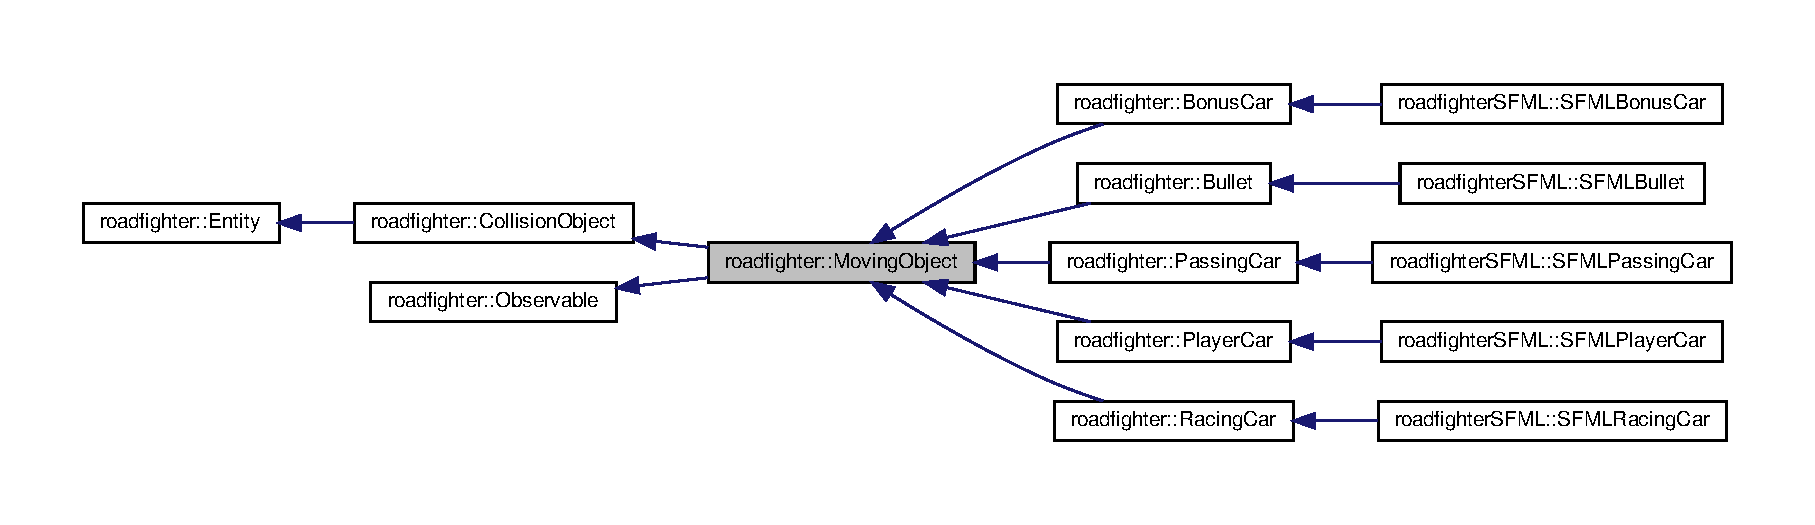
\includegraphics[width=350pt]{classroadfighter_1_1MovingObject__inherit__graph}
\end{center}
\end{figure}


Collaboration diagram for roadfighter\+:\+:Moving\+Object\+:
\nopagebreak
\begin{figure}[H]
\begin{center}
\leavevmode
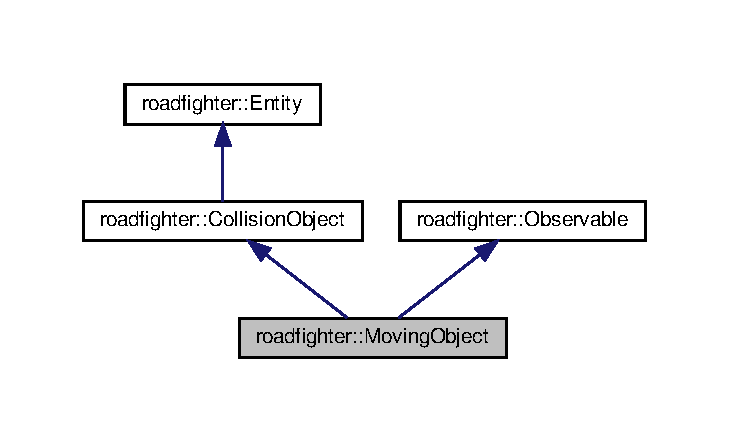
\includegraphics[width=350pt]{classroadfighter_1_1MovingObject__coll__graph}
\end{center}
\end{figure}
\subsection*{Public Member Functions}
\begin{DoxyCompactItemize}
\item 
\hyperlink{classroadfighter_1_1MovingObject_acd1afb2c2845299fc2b6a7e729368ba9}{Moving\+Object} ()=default
\item 
\hyperlink{classroadfighter_1_1MovingObject_ae9c48dc389d0a594ea7bd108849e467f}{Moving\+Object} (const \hyperlink{classroadfighter_1_1MovingObject}{Moving\+Object} \&copy)=default
\item 
\hyperlink{classroadfighter_1_1MovingObject_a759ad597bca6a44c49adf7082fe44469}{Moving\+Object} (\hyperlink{classroadfighter_1_1MovingObject}{Moving\+Object} \&\&move)=default
\item 
\hyperlink{classroadfighter_1_1MovingObject_a5da76d54101b6f2847dc9cdde8dd40cf}{Moving\+Object} (const \hyperlink{classroadfighter_1_1Location}{Location} \&m\+\_\+loc1, const \hyperlink{classroadfighter_1_1Location}{Location} \&m\+\_\+loc2, double m\+\_\+max\+Vert\+Speed, double m\+\_\+vert\+Accel, double m\+\_\+hor\+Accel)
\item 
\hyperlink{classroadfighter_1_1MovingObject}{Moving\+Object} \& \hyperlink{classroadfighter_1_1MovingObject_a46d710b11219a0e973eb1e4d3b375851}{operator=} (const \hyperlink{classroadfighter_1_1MovingObject}{Moving\+Object} \&other)=default
\item 
\hyperlink{classroadfighter_1_1MovingObject}{Moving\+Object} \& \hyperlink{classroadfighter_1_1MovingObject_ae2150a0937d9e1b978bcdf2ba1628677}{operator=} (\hyperlink{classroadfighter_1_1MovingObject}{Moving\+Object} \&\&other)=default
\item 
\hyperlink{classroadfighter_1_1MovingObject_aabb801baf353d53a36998983abbb803a}{$\sim$\+Moving\+Object} () override=default
\item 
virtual void \hyperlink{classroadfighter_1_1MovingObject_ac9f197ee0e91754d2fd653c0b8c84c57}{stop} ()
\item 
virtual void \hyperlink{classroadfighter_1_1MovingObject_ab516489c0569b625c41a1bb9cac19d97}{accelerate} (double dt)
\item 
void \hyperlink{classroadfighter_1_1MovingObject_a7382aeb5c2e7254dde2cc571c85a8fbb}{set\+Vertical\+Speed} (double m\+\_\+\+Vertical\+Speed)
\item 
void \hyperlink{classroadfighter_1_1MovingObject_a9aa56ab17060aabcae8604633993323f}{set\+Vertical\+Speed\+Unbounded} (double m\+\_\+\+Vertical\+Speed)
\item 
void \hyperlink{classroadfighter_1_1MovingObject_a20321fab6dfee452486f80d744d7002d}{set\+Horizontal\+Speed} (double Horizontal\+Speed)
\item 
void \hyperlink{classroadfighter_1_1MovingObject_ac1918d96dac118c4bd7d99168d92867c}{update\+Movement} (double dt) override
\item 
double \hyperlink{classroadfighter_1_1MovingObject_a26e23531dea4a66777f7a3fd61fa4a21}{get\+Horizontal\+Speed} () const
\item 
double \hyperlink{classroadfighter_1_1MovingObject_a50a29cec3ac0234325691f2efd0e7fe1}{get\+Vertical\+Speed} () const
\item 
double \hyperlink{classroadfighter_1_1MovingObject_a299e4d456864595ba066c89f7de58afe}{get\+Vert\+Accel} () const
\item 
double \hyperlink{classroadfighter_1_1MovingObject_a00ed8d1d735142a802792954089e2081}{get\+Hor\+Accel} () const
\item 
E\+Status \hyperlink{classroadfighter_1_1MovingObject_a05cbcd45fb2827a26f54500a897862b4}{get\+Status} () const
\item 
void \hyperlink{classroadfighter_1_1MovingObject_ab1f380b45e20697c45b6ed7b466ca0e9}{set\+Status} (E\+Status m\+\_\+status)
\item 
int \hyperlink{classroadfighter_1_1MovingObject_a447e1cfbdca177040016cd25f736d7df}{get\+Time\+Out} () const
\item 
void \hyperlink{classroadfighter_1_1MovingObject_a3e0c64a4f67f03e84fc388127123c2df}{set\+Time\+Out} (int m\+\_\+time\+Out)
\item 
void \hyperlink{classroadfighter_1_1MovingObject_aa968b69523ee3cfe64fcd5342732ba5a}{decrement\+Time\+Out} ()
\item 
void \hyperlink{classroadfighter_1_1MovingObject_a2c5d69054a59fc5c6d7458f864ee9d57}{update\+Logic} () override
\item 
void \hyperlink{classroadfighter_1_1MovingObject_a193dbc310915e3f81071170b3250516e}{set\+Max\+Vert\+Speed} (double m\+\_\+max\+Vert\+Speed)
\item 
void \hyperlink{classroadfighter_1_1MovingObject_a47bcc94c24b3b6b047ecf45c22574d09}{set\+Hor\+Accel} (double m\+\_\+hor\+Accel)
\item 
void \hyperlink{classroadfighter_1_1MovingObject_a52313182d28796bf27762047c8b289fd}{set\+Vert\+Accel} (double m\+\_\+vert\+Accel)
\item 
double \hyperlink{classroadfighter_1_1MovingObject_a5291cd441cc9b4f4650ff14c584f28d2}{get\+Max\+Vert\+Speed} () const
\end{DoxyCompactItemize}


\subsection{Constructor \& Destructor Documentation}
\mbox{\Hypertarget{classroadfighter_1_1MovingObject_acd1afb2c2845299fc2b6a7e729368ba9}\label{classroadfighter_1_1MovingObject_acd1afb2c2845299fc2b6a7e729368ba9}} 
\index{roadfighter\+::\+Moving\+Object@{roadfighter\+::\+Moving\+Object}!Moving\+Object@{Moving\+Object}}
\index{Moving\+Object@{Moving\+Object}!roadfighter\+::\+Moving\+Object@{roadfighter\+::\+Moving\+Object}}
\subsubsection{\texorpdfstring{Moving\+Object()}{MovingObject()}\hspace{0.1cm}{\footnotesize\ttfamily [1/4]}}
{\footnotesize\ttfamily roadfighter\+::\+Moving\+Object\+::\+Moving\+Object (\begin{DoxyParamCaption}{ }\end{DoxyParamCaption})\hspace{0.3cm}{\ttfamily [default]}}

default constructor for Car \mbox{\Hypertarget{classroadfighter_1_1MovingObject_ae9c48dc389d0a594ea7bd108849e467f}\label{classroadfighter_1_1MovingObject_ae9c48dc389d0a594ea7bd108849e467f}} 
\index{roadfighter\+::\+Moving\+Object@{roadfighter\+::\+Moving\+Object}!Moving\+Object@{Moving\+Object}}
\index{Moving\+Object@{Moving\+Object}!roadfighter\+::\+Moving\+Object@{roadfighter\+::\+Moving\+Object}}
\subsubsection{\texorpdfstring{Moving\+Object()}{MovingObject()}\hspace{0.1cm}{\footnotesize\ttfamily [2/4]}}
{\footnotesize\ttfamily roadfighter\+::\+Moving\+Object\+::\+Moving\+Object (\begin{DoxyParamCaption}\item[{const \hyperlink{classroadfighter_1_1MovingObject}{Moving\+Object} \&}]{copy }\end{DoxyParamCaption})\hspace{0.3cm}{\ttfamily [default]}}

copy constructor 
\begin{DoxyParams}{Parameters}
{\em copy} & the other Car that is being copied \\
\hline
\end{DoxyParams}
\mbox{\Hypertarget{classroadfighter_1_1MovingObject_a759ad597bca6a44c49adf7082fe44469}\label{classroadfighter_1_1MovingObject_a759ad597bca6a44c49adf7082fe44469}} 
\index{roadfighter\+::\+Moving\+Object@{roadfighter\+::\+Moving\+Object}!Moving\+Object@{Moving\+Object}}
\index{Moving\+Object@{Moving\+Object}!roadfighter\+::\+Moving\+Object@{roadfighter\+::\+Moving\+Object}}
\subsubsection{\texorpdfstring{Moving\+Object()}{MovingObject()}\hspace{0.1cm}{\footnotesize\ttfamily [3/4]}}
{\footnotesize\ttfamily roadfighter\+::\+Moving\+Object\+::\+Moving\+Object (\begin{DoxyParamCaption}\item[{\hyperlink{classroadfighter_1_1MovingObject}{Moving\+Object} \&\&}]{move }\end{DoxyParamCaption})\hspace{0.3cm}{\ttfamily [default]}}

move constructor 
\begin{DoxyParams}{Parameters}
{\em Move} & the other Car that is being moved in this one \\
\hline
\end{DoxyParams}
\mbox{\Hypertarget{classroadfighter_1_1MovingObject_a5da76d54101b6f2847dc9cdde8dd40cf}\label{classroadfighter_1_1MovingObject_a5da76d54101b6f2847dc9cdde8dd40cf}} 
\index{roadfighter\+::\+Moving\+Object@{roadfighter\+::\+Moving\+Object}!Moving\+Object@{Moving\+Object}}
\index{Moving\+Object@{Moving\+Object}!roadfighter\+::\+Moving\+Object@{roadfighter\+::\+Moving\+Object}}
\subsubsection{\texorpdfstring{Moving\+Object()}{MovingObject()}\hspace{0.1cm}{\footnotesize\ttfamily [4/4]}}
{\footnotesize\ttfamily roadfighter\+::\+Moving\+Object\+::\+Moving\+Object (\begin{DoxyParamCaption}\item[{const \hyperlink{classroadfighter_1_1Location}{Location} \&}]{m\+\_\+loc1,  }\item[{const \hyperlink{classroadfighter_1_1Location}{Location} \&}]{m\+\_\+loc2,  }\item[{double}]{m\+\_\+max\+Vert\+Speed,  }\item[{double}]{m\+\_\+vert\+Accel,  }\item[{double}]{m\+\_\+hor\+Accel }\end{DoxyParamCaption})}

constructor where all the parameters are given 
\begin{DoxyParams}{Parameters}
{\em m\+\_\+loc1} & first location \\
\hline
{\em m\+\_\+loc2} & second location \\
\hline
{\em m\+\_\+max\+Vert\+Speed} & \\
\hline
{\em m\+\_\+vert\+Accel} & \\
\hline
{\em m\+\_\+hor\+Accel} & \\
\hline
\end{DoxyParams}
\begin{DoxyReturn}{Returns}
none 
\end{DoxyReturn}

\begin{DoxyExceptions}{Exceptions}
{\em none} & \\
\hline
\end{DoxyExceptions}
\mbox{\Hypertarget{classroadfighter_1_1MovingObject_aabb801baf353d53a36998983abbb803a}\label{classroadfighter_1_1MovingObject_aabb801baf353d53a36998983abbb803a}} 
\index{roadfighter\+::\+Moving\+Object@{roadfighter\+::\+Moving\+Object}!````~Moving\+Object@{$\sim$\+Moving\+Object}}
\index{````~Moving\+Object@{$\sim$\+Moving\+Object}!roadfighter\+::\+Moving\+Object@{roadfighter\+::\+Moving\+Object}}
\subsubsection{\texorpdfstring{$\sim$\+Moving\+Object()}{~MovingObject()}}
{\footnotesize\ttfamily roadfighter\+::\+Moving\+Object\+::$\sim$\+Moving\+Object (\begin{DoxyParamCaption}{ }\end{DoxyParamCaption})\hspace{0.3cm}{\ttfamily [override]}, {\ttfamily [default]}}

destructor for Car 

\subsection{Member Function Documentation}
\mbox{\Hypertarget{classroadfighter_1_1MovingObject_ab516489c0569b625c41a1bb9cac19d97}\label{classroadfighter_1_1MovingObject_ab516489c0569b625c41a1bb9cac19d97}} 
\index{roadfighter\+::\+Moving\+Object@{roadfighter\+::\+Moving\+Object}!accelerate@{accelerate}}
\index{accelerate@{accelerate}!roadfighter\+::\+Moving\+Object@{roadfighter\+::\+Moving\+Object}}
\subsubsection{\texorpdfstring{accelerate()}{accelerate()}}
{\footnotesize\ttfamily void roadfighter\+::\+Moving\+Object\+::accelerate (\begin{DoxyParamCaption}\item[{double}]{dt }\end{DoxyParamCaption})\hspace{0.3cm}{\ttfamily [virtual]}}

a function that accelerates the car with the verticalaccel$\ast$dt 
\begin{DoxyParams}{Parameters}
{\em dt} & teh amount of a tick that has passed since previous one \\
\hline
\end{DoxyParams}
\begin{DoxyReturn}{Returns}
none  none 
\end{DoxyReturn}
\mbox{\Hypertarget{classroadfighter_1_1MovingObject_aa968b69523ee3cfe64fcd5342732ba5a}\label{classroadfighter_1_1MovingObject_aa968b69523ee3cfe64fcd5342732ba5a}} 
\index{roadfighter\+::\+Moving\+Object@{roadfighter\+::\+Moving\+Object}!decrement\+Time\+Out@{decrement\+Time\+Out}}
\index{decrement\+Time\+Out@{decrement\+Time\+Out}!roadfighter\+::\+Moving\+Object@{roadfighter\+::\+Moving\+Object}}
\subsubsection{\texorpdfstring{decrement\+Time\+Out()}{decrementTimeOut()}}
{\footnotesize\ttfamily void roadfighter\+::\+Moving\+Object\+::decrement\+Time\+Out (\begin{DoxyParamCaption}{ }\end{DoxyParamCaption})}

a function that subtracts one of the timeout \begin{DoxyReturn}{Returns}
none 
\end{DoxyReturn}

\begin{DoxyExceptions}{Exceptions}
{\em none} & \\
\hline
\end{DoxyExceptions}
\mbox{\Hypertarget{classroadfighter_1_1MovingObject_a00ed8d1d735142a802792954089e2081}\label{classroadfighter_1_1MovingObject_a00ed8d1d735142a802792954089e2081}} 
\index{roadfighter\+::\+Moving\+Object@{roadfighter\+::\+Moving\+Object}!get\+Hor\+Accel@{get\+Hor\+Accel}}
\index{get\+Hor\+Accel@{get\+Hor\+Accel}!roadfighter\+::\+Moving\+Object@{roadfighter\+::\+Moving\+Object}}
\subsubsection{\texorpdfstring{get\+Hor\+Accel()}{getHorAccel()}}
{\footnotesize\ttfamily double roadfighter\+::\+Moving\+Object\+::get\+Hor\+Accel (\begin{DoxyParamCaption}{ }\end{DoxyParamCaption}) const}

getter for horizontal acceleration \begin{DoxyReturn}{Returns}
double 
\end{DoxyReturn}

\begin{DoxyExceptions}{Exceptions}
{\em none} & \\
\hline
\end{DoxyExceptions}
\mbox{\Hypertarget{classroadfighter_1_1MovingObject_a26e23531dea4a66777f7a3fd61fa4a21}\label{classroadfighter_1_1MovingObject_a26e23531dea4a66777f7a3fd61fa4a21}} 
\index{roadfighter\+::\+Moving\+Object@{roadfighter\+::\+Moving\+Object}!get\+Horizontal\+Speed@{get\+Horizontal\+Speed}}
\index{get\+Horizontal\+Speed@{get\+Horizontal\+Speed}!roadfighter\+::\+Moving\+Object@{roadfighter\+::\+Moving\+Object}}
\subsubsection{\texorpdfstring{get\+Horizontal\+Speed()}{getHorizontalSpeed()}}
{\footnotesize\ttfamily double roadfighter\+::\+Moving\+Object\+::get\+Horizontal\+Speed (\begin{DoxyParamCaption}{ }\end{DoxyParamCaption}) const}

getter for the current horizontalspeed \begin{DoxyReturn}{Returns}
a double 
\end{DoxyReturn}

\begin{DoxyExceptions}{Exceptions}
{\em none} & \\
\hline
\end{DoxyExceptions}
\mbox{\Hypertarget{classroadfighter_1_1MovingObject_a5291cd441cc9b4f4650ff14c584f28d2}\label{classroadfighter_1_1MovingObject_a5291cd441cc9b4f4650ff14c584f28d2}} 
\index{roadfighter\+::\+Moving\+Object@{roadfighter\+::\+Moving\+Object}!get\+Max\+Vert\+Speed@{get\+Max\+Vert\+Speed}}
\index{get\+Max\+Vert\+Speed@{get\+Max\+Vert\+Speed}!roadfighter\+::\+Moving\+Object@{roadfighter\+::\+Moving\+Object}}
\subsubsection{\texorpdfstring{get\+Max\+Vert\+Speed()}{getMaxVertSpeed()}}
{\footnotesize\ttfamily double roadfighter\+::\+Moving\+Object\+::get\+Max\+Vert\+Speed (\begin{DoxyParamCaption}{ }\end{DoxyParamCaption}) const}

getter for the maximum vertical speed \begin{DoxyReturn}{Returns}
the max vertical speed  none 
\end{DoxyReturn}
\mbox{\Hypertarget{classroadfighter_1_1MovingObject_a05cbcd45fb2827a26f54500a897862b4}\label{classroadfighter_1_1MovingObject_a05cbcd45fb2827a26f54500a897862b4}} 
\index{roadfighter\+::\+Moving\+Object@{roadfighter\+::\+Moving\+Object}!get\+Status@{get\+Status}}
\index{get\+Status@{get\+Status}!roadfighter\+::\+Moving\+Object@{roadfighter\+::\+Moving\+Object}}
\subsubsection{\texorpdfstring{get\+Status()}{getStatus()}}
{\footnotesize\ttfamily E\+Status roadfighter\+::\+Moving\+Object\+::get\+Status (\begin{DoxyParamCaption}{ }\end{DoxyParamCaption}) const}

getter for current status of the moving object \begin{DoxyReturn}{Returns}
an E\+Status enum 
\end{DoxyReturn}

\begin{DoxyExceptions}{Exceptions}
{\em none} & \\
\hline
\end{DoxyExceptions}
\mbox{\Hypertarget{classroadfighter_1_1MovingObject_a447e1cfbdca177040016cd25f736d7df}\label{classroadfighter_1_1MovingObject_a447e1cfbdca177040016cd25f736d7df}} 
\index{roadfighter\+::\+Moving\+Object@{roadfighter\+::\+Moving\+Object}!get\+Time\+Out@{get\+Time\+Out}}
\index{get\+Time\+Out@{get\+Time\+Out}!roadfighter\+::\+Moving\+Object@{roadfighter\+::\+Moving\+Object}}
\subsubsection{\texorpdfstring{get\+Time\+Out()}{getTimeOut()}}
{\footnotesize\ttfamily int roadfighter\+::\+Moving\+Object\+::get\+Time\+Out (\begin{DoxyParamCaption}{ }\end{DoxyParamCaption}) const}

getter for the current time\+Out \begin{DoxyReturn}{Returns}
an int 
\end{DoxyReturn}

\begin{DoxyExceptions}{Exceptions}
{\em none} & \\
\hline
\end{DoxyExceptions}
\mbox{\Hypertarget{classroadfighter_1_1MovingObject_a299e4d456864595ba066c89f7de58afe}\label{classroadfighter_1_1MovingObject_a299e4d456864595ba066c89f7de58afe}} 
\index{roadfighter\+::\+Moving\+Object@{roadfighter\+::\+Moving\+Object}!get\+Vert\+Accel@{get\+Vert\+Accel}}
\index{get\+Vert\+Accel@{get\+Vert\+Accel}!roadfighter\+::\+Moving\+Object@{roadfighter\+::\+Moving\+Object}}
\subsubsection{\texorpdfstring{get\+Vert\+Accel()}{getVertAccel()}}
{\footnotesize\ttfamily double roadfighter\+::\+Moving\+Object\+::get\+Vert\+Accel (\begin{DoxyParamCaption}{ }\end{DoxyParamCaption}) const}

getter for vertical acceleration \begin{DoxyReturn}{Returns}
double 
\end{DoxyReturn}

\begin{DoxyExceptions}{Exceptions}
{\em none} & \\
\hline
\end{DoxyExceptions}
\mbox{\Hypertarget{classroadfighter_1_1MovingObject_a50a29cec3ac0234325691f2efd0e7fe1}\label{classroadfighter_1_1MovingObject_a50a29cec3ac0234325691f2efd0e7fe1}} 
\index{roadfighter\+::\+Moving\+Object@{roadfighter\+::\+Moving\+Object}!get\+Vertical\+Speed@{get\+Vertical\+Speed}}
\index{get\+Vertical\+Speed@{get\+Vertical\+Speed}!roadfighter\+::\+Moving\+Object@{roadfighter\+::\+Moving\+Object}}
\subsubsection{\texorpdfstring{get\+Vertical\+Speed()}{getVerticalSpeed()}}
{\footnotesize\ttfamily double roadfighter\+::\+Moving\+Object\+::get\+Vertical\+Speed (\begin{DoxyParamCaption}{ }\end{DoxyParamCaption}) const}

getter for current vertical speed \begin{DoxyReturn}{Returns}
a double 
\end{DoxyReturn}

\begin{DoxyExceptions}{Exceptions}
{\em none} & \\
\hline
\end{DoxyExceptions}
\mbox{\Hypertarget{classroadfighter_1_1MovingObject_a46d710b11219a0e973eb1e4d3b375851}\label{classroadfighter_1_1MovingObject_a46d710b11219a0e973eb1e4d3b375851}} 
\index{roadfighter\+::\+Moving\+Object@{roadfighter\+::\+Moving\+Object}!operator=@{operator=}}
\index{operator=@{operator=}!roadfighter\+::\+Moving\+Object@{roadfighter\+::\+Moving\+Object}}
\subsubsection{\texorpdfstring{operator=()}{operator=()}\hspace{0.1cm}{\footnotesize\ttfamily [1/2]}}
{\footnotesize\ttfamily \hyperlink{classroadfighter_1_1MovingObject}{Moving\+Object}\& roadfighter\+::\+Moving\+Object\+::operator= (\begin{DoxyParamCaption}\item[{const \hyperlink{classroadfighter_1_1MovingObject}{Moving\+Object} \&}]{other }\end{DoxyParamCaption})\hspace{0.3cm}{\ttfamily [default]}}

copy assigment for Car 
\begin{DoxyParams}{Parameters}
{\em other} & the Car that is being copied \\
\hline
\end{DoxyParams}
\begin{DoxyReturn}{Returns}
a new Car that is equal to the other one 
\end{DoxyReturn}
\mbox{\Hypertarget{classroadfighter_1_1MovingObject_ae2150a0937d9e1b978bcdf2ba1628677}\label{classroadfighter_1_1MovingObject_ae2150a0937d9e1b978bcdf2ba1628677}} 
\index{roadfighter\+::\+Moving\+Object@{roadfighter\+::\+Moving\+Object}!operator=@{operator=}}
\index{operator=@{operator=}!roadfighter\+::\+Moving\+Object@{roadfighter\+::\+Moving\+Object}}
\subsubsection{\texorpdfstring{operator=()}{operator=()}\hspace{0.1cm}{\footnotesize\ttfamily [2/2]}}
{\footnotesize\ttfamily \hyperlink{classroadfighter_1_1MovingObject}{Moving\+Object}\& roadfighter\+::\+Moving\+Object\+::operator= (\begin{DoxyParamCaption}\item[{\hyperlink{classroadfighter_1_1MovingObject}{Moving\+Object} \&\&}]{other }\end{DoxyParamCaption})\hspace{0.3cm}{\ttfamily [default]}}

move assignment for Car 
\begin{DoxyParams}{Parameters}
{\em other} & other Car that is being moved \\
\hline
\end{DoxyParams}
\begin{DoxyReturn}{Returns}
a Car that contains all the data of the first one 
\end{DoxyReturn}
\mbox{\Hypertarget{classroadfighter_1_1MovingObject_a47bcc94c24b3b6b047ecf45c22574d09}\label{classroadfighter_1_1MovingObject_a47bcc94c24b3b6b047ecf45c22574d09}} 
\index{roadfighter\+::\+Moving\+Object@{roadfighter\+::\+Moving\+Object}!set\+Hor\+Accel@{set\+Hor\+Accel}}
\index{set\+Hor\+Accel@{set\+Hor\+Accel}!roadfighter\+::\+Moving\+Object@{roadfighter\+::\+Moving\+Object}}
\subsubsection{\texorpdfstring{set\+Hor\+Accel()}{setHorAccel()}}
{\footnotesize\ttfamily void roadfighter\+::\+Moving\+Object\+::set\+Hor\+Accel (\begin{DoxyParamCaption}\item[{double}]{m\+\_\+hor\+Accel }\end{DoxyParamCaption})}

setter for the current horizontal acceleration 
\begin{DoxyParams}{Parameters}
{\em m\+\_\+hor\+Accel} & the new horizontal acceleration \\
\hline
\end{DoxyParams}
\begin{DoxyReturn}{Returns}
none 
\end{DoxyReturn}

\begin{DoxyExceptions}{Exceptions}
{\em none} & \\
\hline
\end{DoxyExceptions}
\mbox{\Hypertarget{classroadfighter_1_1MovingObject_a20321fab6dfee452486f80d744d7002d}\label{classroadfighter_1_1MovingObject_a20321fab6dfee452486f80d744d7002d}} 
\index{roadfighter\+::\+Moving\+Object@{roadfighter\+::\+Moving\+Object}!set\+Horizontal\+Speed@{set\+Horizontal\+Speed}}
\index{set\+Horizontal\+Speed@{set\+Horizontal\+Speed}!roadfighter\+::\+Moving\+Object@{roadfighter\+::\+Moving\+Object}}
\subsubsection{\texorpdfstring{set\+Horizontal\+Speed()}{setHorizontalSpeed()}}
{\footnotesize\ttfamily void roadfighter\+::\+Moving\+Object\+::set\+Horizontal\+Speed (\begin{DoxyParamCaption}\item[{double}]{Horizontal\+Speed }\end{DoxyParamCaption})}

setter for horizontalspeed 
\begin{DoxyParams}{Parameters}
{\em m\+\_\+\+Horizontal\+Speed} & the new horizontalspeed \\
\hline
\end{DoxyParams}
\begin{DoxyReturn}{Returns}
none 
\end{DoxyReturn}

\begin{DoxyExceptions}{Exceptions}
{\em none} & \\
\hline
\end{DoxyExceptions}
\mbox{\Hypertarget{classroadfighter_1_1MovingObject_a193dbc310915e3f81071170b3250516e}\label{classroadfighter_1_1MovingObject_a193dbc310915e3f81071170b3250516e}} 
\index{roadfighter\+::\+Moving\+Object@{roadfighter\+::\+Moving\+Object}!set\+Max\+Vert\+Speed@{set\+Max\+Vert\+Speed}}
\index{set\+Max\+Vert\+Speed@{set\+Max\+Vert\+Speed}!roadfighter\+::\+Moving\+Object@{roadfighter\+::\+Moving\+Object}}
\subsubsection{\texorpdfstring{set\+Max\+Vert\+Speed()}{setMaxVertSpeed()}}
{\footnotesize\ttfamily void roadfighter\+::\+Moving\+Object\+::set\+Max\+Vert\+Speed (\begin{DoxyParamCaption}\item[{double}]{m\+\_\+max\+Vert\+Speed }\end{DoxyParamCaption})}

setter for the maxvertspeed 
\begin{DoxyParams}{Parameters}
{\em m\+\_\+max\+Vert\+Speed} & the new max speed \\
\hline
\end{DoxyParams}
\begin{DoxyReturn}{Returns}
none  none 
\end{DoxyReturn}
\mbox{\Hypertarget{classroadfighter_1_1MovingObject_ab1f380b45e20697c45b6ed7b466ca0e9}\label{classroadfighter_1_1MovingObject_ab1f380b45e20697c45b6ed7b466ca0e9}} 
\index{roadfighter\+::\+Moving\+Object@{roadfighter\+::\+Moving\+Object}!set\+Status@{set\+Status}}
\index{set\+Status@{set\+Status}!roadfighter\+::\+Moving\+Object@{roadfighter\+::\+Moving\+Object}}
\subsubsection{\texorpdfstring{set\+Status()}{setStatus()}}
{\footnotesize\ttfamily void roadfighter\+::\+Moving\+Object\+::set\+Status (\begin{DoxyParamCaption}\item[{E\+Status}]{m\+\_\+status }\end{DoxyParamCaption})}

setter for the status 
\begin{DoxyParams}{Parameters}
{\em m\+\_\+status} & an E\+Status enum \\
\hline
\end{DoxyParams}
\begin{DoxyReturn}{Returns}
none 
\end{DoxyReturn}

\begin{DoxyExceptions}{Exceptions}
{\em none} & \\
\hline
\end{DoxyExceptions}
\mbox{\Hypertarget{classroadfighter_1_1MovingObject_a3e0c64a4f67f03e84fc388127123c2df}\label{classroadfighter_1_1MovingObject_a3e0c64a4f67f03e84fc388127123c2df}} 
\index{roadfighter\+::\+Moving\+Object@{roadfighter\+::\+Moving\+Object}!set\+Time\+Out@{set\+Time\+Out}}
\index{set\+Time\+Out@{set\+Time\+Out}!roadfighter\+::\+Moving\+Object@{roadfighter\+::\+Moving\+Object}}
\subsubsection{\texorpdfstring{set\+Time\+Out()}{setTimeOut()}}
{\footnotesize\ttfamily void roadfighter\+::\+Moving\+Object\+::set\+Time\+Out (\begin{DoxyParamCaption}\item[{int}]{m\+\_\+time\+Out }\end{DoxyParamCaption})}

setter for the timeout 
\begin{DoxyParams}{Parameters}
{\em m\+\_\+time\+Out} & an int \\
\hline
\end{DoxyParams}
\begin{DoxyReturn}{Returns}
none 
\end{DoxyReturn}

\begin{DoxyExceptions}{Exceptions}
{\em none} & \\
\hline
\end{DoxyExceptions}
\mbox{\Hypertarget{classroadfighter_1_1MovingObject_a52313182d28796bf27762047c8b289fd}\label{classroadfighter_1_1MovingObject_a52313182d28796bf27762047c8b289fd}} 
\index{roadfighter\+::\+Moving\+Object@{roadfighter\+::\+Moving\+Object}!set\+Vert\+Accel@{set\+Vert\+Accel}}
\index{set\+Vert\+Accel@{set\+Vert\+Accel}!roadfighter\+::\+Moving\+Object@{roadfighter\+::\+Moving\+Object}}
\subsubsection{\texorpdfstring{set\+Vert\+Accel()}{setVertAccel()}}
{\footnotesize\ttfamily void roadfighter\+::\+Moving\+Object\+::set\+Vert\+Accel (\begin{DoxyParamCaption}\item[{double}]{m\+\_\+vert\+Accel }\end{DoxyParamCaption})}

setter for the vertical acceleration 
\begin{DoxyParams}{Parameters}
{\em m\+\_\+vert\+Accel} & the new vertical accelertaion \\
\hline
\end{DoxyParams}
\begin{DoxyReturn}{Returns}
none 
\end{DoxyReturn}

\begin{DoxyExceptions}{Exceptions}
{\em none} & \\
\hline
\end{DoxyExceptions}
\mbox{\Hypertarget{classroadfighter_1_1MovingObject_a7382aeb5c2e7254dde2cc571c85a8fbb}\label{classroadfighter_1_1MovingObject_a7382aeb5c2e7254dde2cc571c85a8fbb}} 
\index{roadfighter\+::\+Moving\+Object@{roadfighter\+::\+Moving\+Object}!set\+Vertical\+Speed@{set\+Vertical\+Speed}}
\index{set\+Vertical\+Speed@{set\+Vertical\+Speed}!roadfighter\+::\+Moving\+Object@{roadfighter\+::\+Moving\+Object}}
\subsubsection{\texorpdfstring{set\+Vertical\+Speed()}{setVerticalSpeed()}}
{\footnotesize\ttfamily void roadfighter\+::\+Moving\+Object\+::set\+Vertical\+Speed (\begin{DoxyParamCaption}\item[{double}]{m\+\_\+\+Vertical\+Speed }\end{DoxyParamCaption})}

setter for verticalspeed 
\begin{DoxyParams}{Parameters}
{\em m\+\_\+\+Vertical\+Speed} & the new verticalspeed \\
\hline
\end{DoxyParams}
\begin{DoxyReturn}{Returns}
none 
\end{DoxyReturn}

\begin{DoxyExceptions}{Exceptions}
{\em none} & \\
\hline
\end{DoxyExceptions}
\mbox{\Hypertarget{classroadfighter_1_1MovingObject_a9aa56ab17060aabcae8604633993323f}\label{classroadfighter_1_1MovingObject_a9aa56ab17060aabcae8604633993323f}} 
\index{roadfighter\+::\+Moving\+Object@{roadfighter\+::\+Moving\+Object}!set\+Vertical\+Speed\+Unbounded@{set\+Vertical\+Speed\+Unbounded}}
\index{set\+Vertical\+Speed\+Unbounded@{set\+Vertical\+Speed\+Unbounded}!roadfighter\+::\+Moving\+Object@{roadfighter\+::\+Moving\+Object}}
\subsubsection{\texorpdfstring{set\+Vertical\+Speed\+Unbounded()}{setVerticalSpeedUnbounded()}}
{\footnotesize\ttfamily void roadfighter\+::\+Moving\+Object\+::set\+Vertical\+Speed\+Unbounded (\begin{DoxyParamCaption}\item[{double}]{m\+\_\+\+Vertical\+Speed }\end{DoxyParamCaption})}

setter for verticalspeed were there is no check if you are above the maxvertspeed 
\begin{DoxyParams}{Parameters}
{\em m\+\_\+\+Vertical\+Speed} & the new verticalspeed \\
\hline
\end{DoxyParams}
\begin{DoxyReturn}{Returns}
none  none 
\end{DoxyReturn}
\mbox{\Hypertarget{classroadfighter_1_1MovingObject_ac9f197ee0e91754d2fd653c0b8c84c57}\label{classroadfighter_1_1MovingObject_ac9f197ee0e91754d2fd653c0b8c84c57}} 
\index{roadfighter\+::\+Moving\+Object@{roadfighter\+::\+Moving\+Object}!stop@{stop}}
\index{stop@{stop}!roadfighter\+::\+Moving\+Object@{roadfighter\+::\+Moving\+Object}}
\subsubsection{\texorpdfstring{stop()}{stop()}}
{\footnotesize\ttfamily void roadfighter\+::\+Moving\+Object\+::stop (\begin{DoxyParamCaption}{ }\end{DoxyParamCaption})\hspace{0.3cm}{\ttfamily [virtual]}}

a function that sets the vertical and horizontal speed to 0 \begin{DoxyReturn}{Returns}
none 
\end{DoxyReturn}

\begin{DoxyExceptions}{Exceptions}
{\em none} & \\
\hline
\end{DoxyExceptions}
\mbox{\Hypertarget{classroadfighter_1_1MovingObject_a2c5d69054a59fc5c6d7458f864ee9d57}\label{classroadfighter_1_1MovingObject_a2c5d69054a59fc5c6d7458f864ee9d57}} 
\index{roadfighter\+::\+Moving\+Object@{roadfighter\+::\+Moving\+Object}!update\+Logic@{update\+Logic}}
\index{update\+Logic@{update\+Logic}!roadfighter\+::\+Moving\+Object@{roadfighter\+::\+Moving\+Object}}
\subsubsection{\texorpdfstring{update\+Logic()}{updateLogic()}}
{\footnotesize\ttfamily void roadfighter\+::\+Moving\+Object\+::update\+Logic (\begin{DoxyParamCaption}{ }\end{DoxyParamCaption})\hspace{0.3cm}{\ttfamily [override]}, {\ttfamily [virtual]}}

this function updates the logic of a movingobject this only means that the verticalspeed gets changed according to the current acceleration \begin{DoxyReturn}{Returns}
none 
\end{DoxyReturn}

\begin{DoxyExceptions}{Exceptions}
{\em none} & \\
\hline
\end{DoxyExceptions}


Implements \hyperlink{classroadfighter_1_1Entity_a54c00f1af306290bae3e4b84e196566b}{roadfighter\+::\+Entity}.



Reimplemented in \hyperlink{classroadfighter_1_1PlayerCar_a01480487ca7978a50a3c6609f1ebe6df}{roadfighter\+::\+Player\+Car}, \hyperlink{classroadfighter_1_1RacingCar_af3f3b4c368ba61c13dc9b99004895c5d}{roadfighter\+::\+Racing\+Car}, and \hyperlink{classroadfighter_1_1PassingCar_ac3fe3087290121bf44880f94efa3a916}{roadfighter\+::\+Passing\+Car}.

\mbox{\Hypertarget{classroadfighter_1_1MovingObject_ac1918d96dac118c4bd7d99168d92867c}\label{classroadfighter_1_1MovingObject_ac1918d96dac118c4bd7d99168d92867c}} 
\index{roadfighter\+::\+Moving\+Object@{roadfighter\+::\+Moving\+Object}!update\+Movement@{update\+Movement}}
\index{update\+Movement@{update\+Movement}!roadfighter\+::\+Moving\+Object@{roadfighter\+::\+Moving\+Object}}
\subsubsection{\texorpdfstring{update\+Movement()}{updateMovement()}}
{\footnotesize\ttfamily void roadfighter\+::\+Moving\+Object\+::update\+Movement (\begin{DoxyParamCaption}\item[{double}]{dt }\end{DoxyParamCaption})\hspace{0.3cm}{\ttfamily [override]}, {\ttfamily [virtual]}}

a function that updates the car 
\begin{DoxyParams}{Parameters}
{\em dt} & the amount of ticks that have passed since the previous one overriden from entity class \\
\hline
\end{DoxyParams}
\begin{DoxyReturn}{Returns}
none 
\end{DoxyReturn}

\begin{DoxyExceptions}{Exceptions}
{\em none} & \\
\hline
\end{DoxyExceptions}


Implements \hyperlink{classroadfighter_1_1Entity_a66614a11004d6f9516473f60b530f689}{roadfighter\+::\+Entity}.



Reimplemented in \hyperlink{classroadfighter_1_1PlayerCar_aa1dcbec01dde1b212e4919b61338edde}{roadfighter\+::\+Player\+Car}, \hyperlink{classroadfighter_1_1PassingCar_ade5ebca5d7dbdb75bd9eee5817972363}{roadfighter\+::\+Passing\+Car}, and \hyperlink{classroadfighter_1_1RacingCar_a2e8f3c63381a1fe432cddcc1f34fb935}{roadfighter\+::\+Racing\+Car}.



The documentation for this class was generated from the following files\+:\begin{DoxyCompactItemize}
\item 
Game\+Logic/include/\+Entities/\hyperlink{MovingObject_8h}{Moving\+Object.\+h}\item 
Game\+Logic/\+Source/\+Entities/\hyperlink{MovingObject_8cpp}{Moving\+Object.\+cpp}\end{DoxyCompactItemize}

\hypertarget{classObservable}{}\section{Observable Class Reference}
\label{classObservable}\index{Observable@{Observable}}


Inheritance diagram for Observable\+:\nopagebreak
\begin{figure}[H]
\begin{center}
\leavevmode
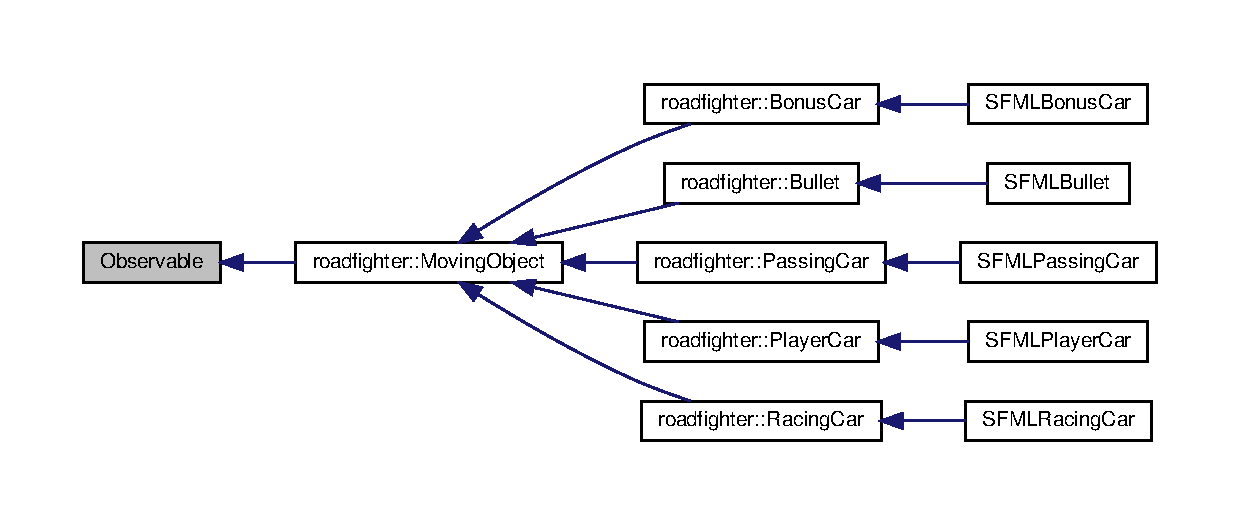
\includegraphics[width=350pt]{classObservable__inherit__graph}
\end{center}
\end{figure}
\subsection*{Public Member Functions}
\begin{DoxyCompactItemize}
\item 
\mbox{\Hypertarget{classObservable_a6b67eac0111f9fd37ee182b0b617421b}\label{classObservable_a6b67eac0111f9fd37ee182b0b617421b}} 
void {\bfseries attach} (std\+::shared\+\_\+ptr$<$ \hyperlink{classObserverBase}{Observer\+Base} $>$ to\+Attach)
\item 
\mbox{\Hypertarget{classObservable_ab0523c2c587f258b3f37976ec4951e35}\label{classObservable_ab0523c2c587f258b3f37976ec4951e35}} 
void {\bfseries detach} ()
\item 
\mbox{\Hypertarget{classObservable_a7dcfb78aab73c197ed731c449454820b}\label{classObservable_a7dcfb78aab73c197ed731c449454820b}} 
virtual void {\bfseries notify} (int amount)
\end{DoxyCompactItemize}


The documentation for this class was generated from the following files\+:\begin{DoxyCompactItemize}
\item 
Game\+Logic/include/\+Observer/Observable.\+h\item 
Game\+Logic/\+Source/\+Observer/Observable.\+cpp\end{DoxyCompactItemize}

\hypertarget{classObserverBase}{}\section{Observer\+Base Class Reference}
\label{classObserverBase}\index{Observer\+Base@{Observer\+Base}}


Inheritance diagram for Observer\+Base\+:\nopagebreak
\begin{figure}[H]
\begin{center}
\leavevmode
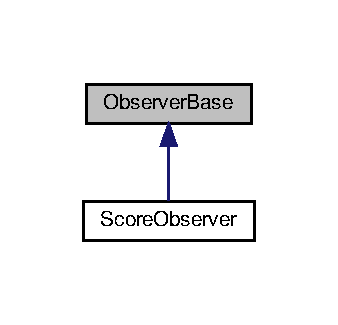
\includegraphics[width=162pt]{classObserverBase__inherit__graph}
\end{center}
\end{figure}
\subsection*{Public Member Functions}
\begin{DoxyCompactItemize}
\item 
\mbox{\Hypertarget{classObserverBase_ae174a3136f06a9e17a7410f02aab1480}\label{classObserverBase_ae174a3136f06a9e17a7410f02aab1480}} 
virtual void {\bfseries update} (int amount)=0
\end{DoxyCompactItemize}


The documentation for this class was generated from the following file\+:\begin{DoxyCompactItemize}
\item 
Game\+Logic/include/\+Observer/Observer\+Base.\+h\end{DoxyCompactItemize}

\hypertarget{classroadfighter_1_1PassingCar}{}\section{roadfighter\+:\+:Passing\+Car Class Reference}
\label{classroadfighter_1_1PassingCar}\index{roadfighter\+::\+Passing\+Car@{roadfighter\+::\+Passing\+Car}}


Inheritance diagram for roadfighter\+:\+:Passing\+Car\+:\nopagebreak
\begin{figure}[H]
\begin{center}
\leavevmode
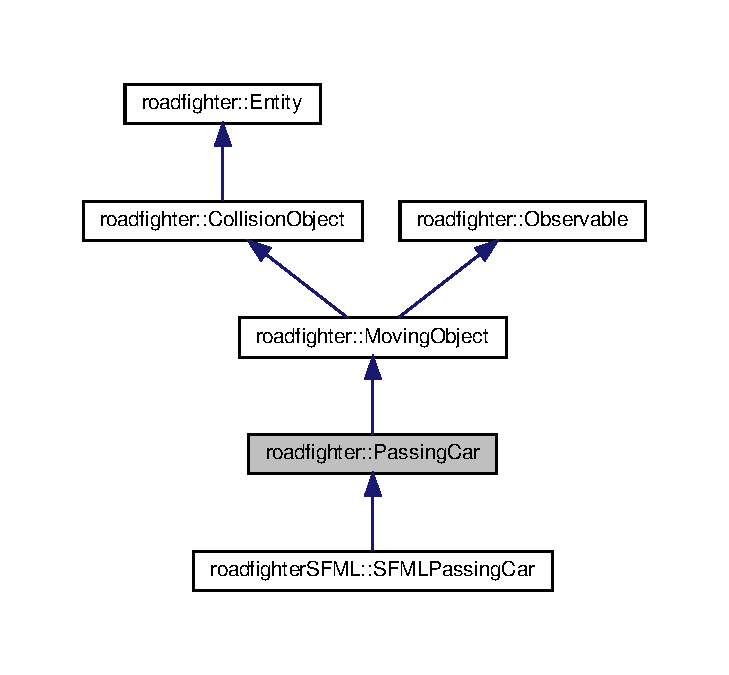
\includegraphics[width=298pt]{classroadfighter_1_1PassingCar__inherit__graph}
\end{center}
\end{figure}


Collaboration diagram for roadfighter\+:\+:Passing\+Car\+:\nopagebreak
\begin{figure}[H]
\begin{center}
\leavevmode
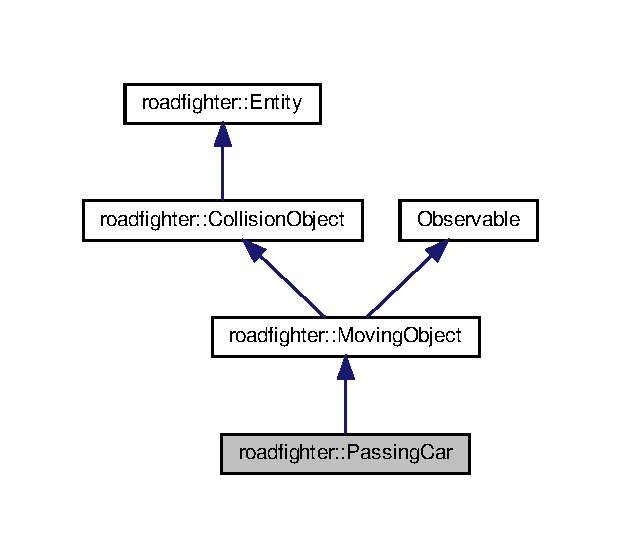
\includegraphics[width=298pt]{classroadfighter_1_1PassingCar__coll__graph}
\end{center}
\end{figure}
\subsection*{Public Member Functions}
\begin{DoxyCompactItemize}
\item 
\hyperlink{classroadfighter_1_1PassingCar_af071c33cd301f1558054423d30b0b0fd}{Passing\+Car} ()=default
\item 
\mbox{\Hypertarget{classroadfighter_1_1PassingCar_a0492e46e1930b2eec14622a61d33acc2}\label{classroadfighter_1_1PassingCar_a0492e46e1930b2eec14622a61d33acc2}} 
{\bfseries Passing\+Car} (const \hyperlink{classroadfighter_1_1Location}{Location} \&m\+\_\+loc1, const \hyperlink{classroadfighter_1_1Location}{Location} \&m\+\_\+loc2, double vert\+Speed)
\item 
\hyperlink{classroadfighter_1_1PassingCar_abf5e19562be7b8d2ff71557fb2027aae}{Passing\+Car} (const \hyperlink{classroadfighter_1_1PassingCar}{Passing\+Car} \&copy)=default
\item 
\hyperlink{classroadfighter_1_1PassingCar_aabea2fb415c816c0308399cd49732d83}{Passing\+Car} (\hyperlink{classroadfighter_1_1PassingCar}{Passing\+Car} \&\&move)=default
\item 
\hyperlink{classroadfighter_1_1PassingCar}{Passing\+Car} \& \hyperlink{classroadfighter_1_1PassingCar_aa3cbe5aa96205e8b7f4ba99531e47735}{operator=} (const \hyperlink{classroadfighter_1_1PassingCar}{Passing\+Car} \&other)=default
\item 
\hyperlink{classroadfighter_1_1PassingCar}{Passing\+Car} \& \hyperlink{classroadfighter_1_1PassingCar_a5cae5b484691e5975d2b9d59254108ad}{operator=} (\hyperlink{classroadfighter_1_1PassingCar}{Passing\+Car} \&\&other)=default
\item 
\hyperlink{classroadfighter_1_1PassingCar_ab590a845658cdb5aae74c0a922548aa8}{$\sim$\+Passing\+Car} () override=default
\item 
void \hyperlink{classroadfighter_1_1PassingCar_ac3fe3087290121bf44880f94efa3a916}{update\+Logic} () override
\item 
void \hyperlink{classroadfighter_1_1PassingCar_ade5ebca5d7dbdb75bd9eee5817972363}{update\+Movement} (double dt) override
\item 
bool \hyperlink{classroadfighter_1_1PassingCar_a96b365c19d4e6e940d3827319434a022}{must\+Delete} () const override
\item 
void \hyperlink{classroadfighter_1_1PassingCar_a04ee71b75c90f21efef591756855bf37}{collide\+With} (std\+::shared\+\_\+ptr$<$ \hyperlink{classroadfighter_1_1CollisionObject}{Collision\+Object} $>$ \&collided) override
\item 
void \hyperlink{classroadfighter_1_1PassingCar_a5c437fb5164d2735881a469650db048d}{crash} () override
\item 
void \hyperlink{classroadfighter_1_1PassingCar_ac04b801b789bf880011d5cdb1ffdec59}{shot} () override
\item 
void \hyperlink{classroadfighter_1_1PassingCar_a43d55e28efe840d81c1b87216920eb69}{bonus} () override
\item 
void \hyperlink{classroadfighter_1_1PassingCar_a365d8befb1c2fd34337fc25665ccc73f}{win} () override
\end{DoxyCompactItemize}


\subsection{Constructor \& Destructor Documentation}
\mbox{\Hypertarget{classroadfighter_1_1PassingCar_af071c33cd301f1558054423d30b0b0fd}\label{classroadfighter_1_1PassingCar_af071c33cd301f1558054423d30b0b0fd}} 
\index{roadfighter\+::\+Passing\+Car@{roadfighter\+::\+Passing\+Car}!Passing\+Car@{Passing\+Car}}
\index{Passing\+Car@{Passing\+Car}!roadfighter\+::\+Passing\+Car@{roadfighter\+::\+Passing\+Car}}
\subsubsection{\texorpdfstring{Passing\+Car()}{PassingCar()}\hspace{0.1cm}{\footnotesize\ttfamily [1/3]}}
{\footnotesize\ttfamily roadfighter\+::\+Passing\+Car\+::\+Passing\+Car (\begin{DoxyParamCaption}{ }\end{DoxyParamCaption})\hspace{0.3cm}{\ttfamily [default]}}

default constructor for \hyperlink{classroadfighter_1_1PassingCar}{Passing\+Car} \mbox{\Hypertarget{classroadfighter_1_1PassingCar_abf5e19562be7b8d2ff71557fb2027aae}\label{classroadfighter_1_1PassingCar_abf5e19562be7b8d2ff71557fb2027aae}} 
\index{roadfighter\+::\+Passing\+Car@{roadfighter\+::\+Passing\+Car}!Passing\+Car@{Passing\+Car}}
\index{Passing\+Car@{Passing\+Car}!roadfighter\+::\+Passing\+Car@{roadfighter\+::\+Passing\+Car}}
\subsubsection{\texorpdfstring{Passing\+Car()}{PassingCar()}\hspace{0.1cm}{\footnotesize\ttfamily [2/3]}}
{\footnotesize\ttfamily roadfighter\+::\+Passing\+Car\+::\+Passing\+Car (\begin{DoxyParamCaption}\item[{const \hyperlink{classroadfighter_1_1PassingCar}{Passing\+Car} \&}]{copy }\end{DoxyParamCaption})\hspace{0.3cm}{\ttfamily [default]}}

copy constructor 
\begin{DoxyParams}{Parameters}
{\em copy} & the other \hyperlink{classroadfighter_1_1PassingCar}{Passing\+Car} that is being copied \\
\hline
\end{DoxyParams}
\mbox{\Hypertarget{classroadfighter_1_1PassingCar_aabea2fb415c816c0308399cd49732d83}\label{classroadfighter_1_1PassingCar_aabea2fb415c816c0308399cd49732d83}} 
\index{roadfighter\+::\+Passing\+Car@{roadfighter\+::\+Passing\+Car}!Passing\+Car@{Passing\+Car}}
\index{Passing\+Car@{Passing\+Car}!roadfighter\+::\+Passing\+Car@{roadfighter\+::\+Passing\+Car}}
\subsubsection{\texorpdfstring{Passing\+Car()}{PassingCar()}\hspace{0.1cm}{\footnotesize\ttfamily [3/3]}}
{\footnotesize\ttfamily roadfighter\+::\+Passing\+Car\+::\+Passing\+Car (\begin{DoxyParamCaption}\item[{\hyperlink{classroadfighter_1_1PassingCar}{Passing\+Car} \&\&}]{move }\end{DoxyParamCaption})\hspace{0.3cm}{\ttfamily [default]}}

move constructor 
\begin{DoxyParams}{Parameters}
{\em Move} & the other \hyperlink{classroadfighter_1_1PassingCar}{Passing\+Car} that is being moved in this one \\
\hline
\end{DoxyParams}
\mbox{\Hypertarget{classroadfighter_1_1PassingCar_ab590a845658cdb5aae74c0a922548aa8}\label{classroadfighter_1_1PassingCar_ab590a845658cdb5aae74c0a922548aa8}} 
\index{roadfighter\+::\+Passing\+Car@{roadfighter\+::\+Passing\+Car}!````~Passing\+Car@{$\sim$\+Passing\+Car}}
\index{````~Passing\+Car@{$\sim$\+Passing\+Car}!roadfighter\+::\+Passing\+Car@{roadfighter\+::\+Passing\+Car}}
\subsubsection{\texorpdfstring{$\sim$\+Passing\+Car()}{~PassingCar()}}
{\footnotesize\ttfamily roadfighter\+::\+Passing\+Car\+::$\sim$\+Passing\+Car (\begin{DoxyParamCaption}{ }\end{DoxyParamCaption})\hspace{0.3cm}{\ttfamily [override]}, {\ttfamily [default]}}

destructor for \hyperlink{classroadfighter_1_1PassingCar}{Passing\+Car} 

\subsection{Member Function Documentation}
\mbox{\Hypertarget{classroadfighter_1_1PassingCar_a43d55e28efe840d81c1b87216920eb69}\label{classroadfighter_1_1PassingCar_a43d55e28efe840d81c1b87216920eb69}} 
\index{roadfighter\+::\+Passing\+Car@{roadfighter\+::\+Passing\+Car}!bonus@{bonus}}
\index{bonus@{bonus}!roadfighter\+::\+Passing\+Car@{roadfighter\+::\+Passing\+Car}}
\subsubsection{\texorpdfstring{bonus()}{bonus()}}
{\footnotesize\ttfamily void roadfighter\+::\+Passing\+Car\+::bonus (\begin{DoxyParamCaption}{ }\end{DoxyParamCaption})\hspace{0.3cm}{\ttfamily [override]}, {\ttfamily [virtual]}}

function that handles what happens when this car gets a bonus 

Implements \hyperlink{classroadfighter_1_1CollisionObject_a157e499c27619ceefd6179a459fafd90}{roadfighter\+::\+Collision\+Object}.

\mbox{\Hypertarget{classroadfighter_1_1PassingCar_a04ee71b75c90f21efef591756855bf37}\label{classroadfighter_1_1PassingCar_a04ee71b75c90f21efef591756855bf37}} 
\index{roadfighter\+::\+Passing\+Car@{roadfighter\+::\+Passing\+Car}!collide\+With@{collide\+With}}
\index{collide\+With@{collide\+With}!roadfighter\+::\+Passing\+Car@{roadfighter\+::\+Passing\+Car}}
\subsubsection{\texorpdfstring{collide\+With()}{collideWith()}}
{\footnotesize\ttfamily void roadfighter\+::\+Passing\+Car\+::collide\+With (\begin{DoxyParamCaption}\item[{std\+::shared\+\_\+ptr$<$ \hyperlink{classroadfighter_1_1CollisionObject}{Collision\+Object} $>$ \&}]{collided }\end{DoxyParamCaption})\hspace{0.3cm}{\ttfamily [override]}, {\ttfamily [virtual]}}

a function that will handle what will happen when a object collides with this one 
\begin{DoxyParams}{Parameters}
{\em collided} & the object this ones collides with \\
\hline
\end{DoxyParams}


Implements \hyperlink{classroadfighter_1_1CollisionObject_a7eafa2fdc4463788b816fdd9370d28d9}{roadfighter\+::\+Collision\+Object}.

\mbox{\Hypertarget{classroadfighter_1_1PassingCar_a5c437fb5164d2735881a469650db048d}\label{classroadfighter_1_1PassingCar_a5c437fb5164d2735881a469650db048d}} 
\index{roadfighter\+::\+Passing\+Car@{roadfighter\+::\+Passing\+Car}!crash@{crash}}
\index{crash@{crash}!roadfighter\+::\+Passing\+Car@{roadfighter\+::\+Passing\+Car}}
\subsubsection{\texorpdfstring{crash()}{crash()}}
{\footnotesize\ttfamily void roadfighter\+::\+Passing\+Car\+::crash (\begin{DoxyParamCaption}{ }\end{DoxyParamCaption})\hspace{0.3cm}{\ttfamily [override]}, {\ttfamily [virtual]}}

function that handles what happens when this car crashes 

Implements \hyperlink{classroadfighter_1_1CollisionObject_a18f0f60a5a664d6fb554daac0d398a2c}{roadfighter\+::\+Collision\+Object}.

\mbox{\Hypertarget{classroadfighter_1_1PassingCar_a96b365c19d4e6e940d3827319434a022}\label{classroadfighter_1_1PassingCar_a96b365c19d4e6e940d3827319434a022}} 
\index{roadfighter\+::\+Passing\+Car@{roadfighter\+::\+Passing\+Car}!must\+Delete@{must\+Delete}}
\index{must\+Delete@{must\+Delete}!roadfighter\+::\+Passing\+Car@{roadfighter\+::\+Passing\+Car}}
\subsubsection{\texorpdfstring{must\+Delete()}{mustDelete()}}
{\footnotesize\ttfamily bool roadfighter\+::\+Passing\+Car\+::must\+Delete (\begin{DoxyParamCaption}{ }\end{DoxyParamCaption}) const\hspace{0.3cm}{\ttfamily [override]}, {\ttfamily [virtual]}}

a function that say whether the car needs to be removed from the game  bool that is true if the car needs to be deletet 

Reimplemented from \hyperlink{classroadfighter_1_1CollisionObject_a738071cd7b1b8cd4c8d455b5e552bd4c}{roadfighter\+::\+Collision\+Object}.

\mbox{\Hypertarget{classroadfighter_1_1PassingCar_aa3cbe5aa96205e8b7f4ba99531e47735}\label{classroadfighter_1_1PassingCar_aa3cbe5aa96205e8b7f4ba99531e47735}} 
\index{roadfighter\+::\+Passing\+Car@{roadfighter\+::\+Passing\+Car}!operator=@{operator=}}
\index{operator=@{operator=}!roadfighter\+::\+Passing\+Car@{roadfighter\+::\+Passing\+Car}}
\subsubsection{\texorpdfstring{operator=()}{operator=()}\hspace{0.1cm}{\footnotesize\ttfamily [1/2]}}
{\footnotesize\ttfamily \hyperlink{classroadfighter_1_1PassingCar}{Passing\+Car}\& roadfighter\+::\+Passing\+Car\+::operator= (\begin{DoxyParamCaption}\item[{const \hyperlink{classroadfighter_1_1PassingCar}{Passing\+Car} \&}]{other }\end{DoxyParamCaption})\hspace{0.3cm}{\ttfamily [default]}}

copy assigment for \hyperlink{classroadfighter_1_1PassingCar}{Passing\+Car} 
\begin{DoxyParams}{Parameters}
{\em other} & the \hyperlink{classroadfighter_1_1PassingCar}{Passing\+Car} that is being copied \\
\hline
\end{DoxyParams}
\begin{DoxyReturn}{Returns}
a new \hyperlink{classroadfighter_1_1PassingCar}{Passing\+Car} that is equal to the other one 
\end{DoxyReturn}
\mbox{\Hypertarget{classroadfighter_1_1PassingCar_a5cae5b484691e5975d2b9d59254108ad}\label{classroadfighter_1_1PassingCar_a5cae5b484691e5975d2b9d59254108ad}} 
\index{roadfighter\+::\+Passing\+Car@{roadfighter\+::\+Passing\+Car}!operator=@{operator=}}
\index{operator=@{operator=}!roadfighter\+::\+Passing\+Car@{roadfighter\+::\+Passing\+Car}}
\subsubsection{\texorpdfstring{operator=()}{operator=()}\hspace{0.1cm}{\footnotesize\ttfamily [2/2]}}
{\footnotesize\ttfamily \hyperlink{classroadfighter_1_1PassingCar}{Passing\+Car}\& roadfighter\+::\+Passing\+Car\+::operator= (\begin{DoxyParamCaption}\item[{\hyperlink{classroadfighter_1_1PassingCar}{Passing\+Car} \&\&}]{other }\end{DoxyParamCaption})\hspace{0.3cm}{\ttfamily [default]}}

move assignment for \hyperlink{classroadfighter_1_1PassingCar}{Passing\+Car} 
\begin{DoxyParams}{Parameters}
{\em other} & other \hyperlink{classroadfighter_1_1PassingCar}{Passing\+Car} that is being moved \\
\hline
\end{DoxyParams}
\begin{DoxyReturn}{Returns}
a \hyperlink{classroadfighter_1_1PassingCar}{Passing\+Car} that contains all the data of the first one 
\end{DoxyReturn}
\mbox{\Hypertarget{classroadfighter_1_1PassingCar_ac04b801b789bf880011d5cdb1ffdec59}\label{classroadfighter_1_1PassingCar_ac04b801b789bf880011d5cdb1ffdec59}} 
\index{roadfighter\+::\+Passing\+Car@{roadfighter\+::\+Passing\+Car}!shot@{shot}}
\index{shot@{shot}!roadfighter\+::\+Passing\+Car@{roadfighter\+::\+Passing\+Car}}
\subsubsection{\texorpdfstring{shot()}{shot()}}
{\footnotesize\ttfamily void roadfighter\+::\+Passing\+Car\+::shot (\begin{DoxyParamCaption}{ }\end{DoxyParamCaption})\hspace{0.3cm}{\ttfamily [override]}, {\ttfamily [virtual]}}

function that handles what happens when this car get shot 

Implements \hyperlink{classroadfighter_1_1CollisionObject_a338a1071e6d5e25439e57c8673308dbb}{roadfighter\+::\+Collision\+Object}.

\mbox{\Hypertarget{classroadfighter_1_1PassingCar_ac3fe3087290121bf44880f94efa3a916}\label{classroadfighter_1_1PassingCar_ac3fe3087290121bf44880f94efa3a916}} 
\index{roadfighter\+::\+Passing\+Car@{roadfighter\+::\+Passing\+Car}!update\+Logic@{update\+Logic}}
\index{update\+Logic@{update\+Logic}!roadfighter\+::\+Passing\+Car@{roadfighter\+::\+Passing\+Car}}
\subsubsection{\texorpdfstring{update\+Logic()}{updateLogic()}}
{\footnotesize\ttfamily void roadfighter\+::\+Passing\+Car\+::update\+Logic (\begin{DoxyParamCaption}{ }\end{DoxyParamCaption})\hspace{0.3cm}{\ttfamily [override]}, {\ttfamily [virtual]}}

update the logic of the passing car 

Reimplemented from \hyperlink{classroadfighter_1_1MovingObject_a2c5d69054a59fc5c6d7458f864ee9d57}{roadfighter\+::\+Moving\+Object}.

\mbox{\Hypertarget{classroadfighter_1_1PassingCar_ade5ebca5d7dbdb75bd9eee5817972363}\label{classroadfighter_1_1PassingCar_ade5ebca5d7dbdb75bd9eee5817972363}} 
\index{roadfighter\+::\+Passing\+Car@{roadfighter\+::\+Passing\+Car}!update\+Movement@{update\+Movement}}
\index{update\+Movement@{update\+Movement}!roadfighter\+::\+Passing\+Car@{roadfighter\+::\+Passing\+Car}}
\subsubsection{\texorpdfstring{update\+Movement()}{updateMovement()}}
{\footnotesize\ttfamily void roadfighter\+::\+Passing\+Car\+::update\+Movement (\begin{DoxyParamCaption}\item[{double}]{dt }\end{DoxyParamCaption})\hspace{0.3cm}{\ttfamily [override]}, {\ttfamily [virtual]}}

update the movement of the passing car with dt ticks 
\begin{DoxyParams}{Parameters}
{\em dt} & the amount of a tick we need to move the car \\
\hline
\end{DoxyParams}


Reimplemented from \hyperlink{classroadfighter_1_1MovingObject_ac1918d96dac118c4bd7d99168d92867c}{roadfighter\+::\+Moving\+Object}.

\mbox{\Hypertarget{classroadfighter_1_1PassingCar_a365d8befb1c2fd34337fc25665ccc73f}\label{classroadfighter_1_1PassingCar_a365d8befb1c2fd34337fc25665ccc73f}} 
\index{roadfighter\+::\+Passing\+Car@{roadfighter\+::\+Passing\+Car}!win@{win}}
\index{win@{win}!roadfighter\+::\+Passing\+Car@{roadfighter\+::\+Passing\+Car}}
\subsubsection{\texorpdfstring{win()}{win()}}
{\footnotesize\ttfamily void roadfighter\+::\+Passing\+Car\+::win (\begin{DoxyParamCaption}{ }\end{DoxyParamCaption})\hspace{0.3cm}{\ttfamily [override]}, {\ttfamily [virtual]}}

function that handles what happens when this car wins 

Implements \hyperlink{classroadfighter_1_1CollisionObject_a03ce1ae52676088839d85c597743052c}{roadfighter\+::\+Collision\+Object}.



The documentation for this class was generated from the following files\+:\begin{DoxyCompactItemize}
\item 
Game\+Logic/include/\+Entities/Passing\+Car.\+h\item 
Game\+Logic/\+Source/\+Entities/Passing\+Car.\+cpp\end{DoxyCompactItemize}

\hypertarget{classroadfighter_1_1PlayerCar}{}\section{roadfighter\+:\+:Player\+Car Class Reference}
\label{classroadfighter_1_1PlayerCar}\index{roadfighter\+::\+Player\+Car@{roadfighter\+::\+Player\+Car}}


Inheritance diagram for roadfighter\+:\+:Player\+Car\+:\nopagebreak
\begin{figure}[H]
\begin{center}
\leavevmode
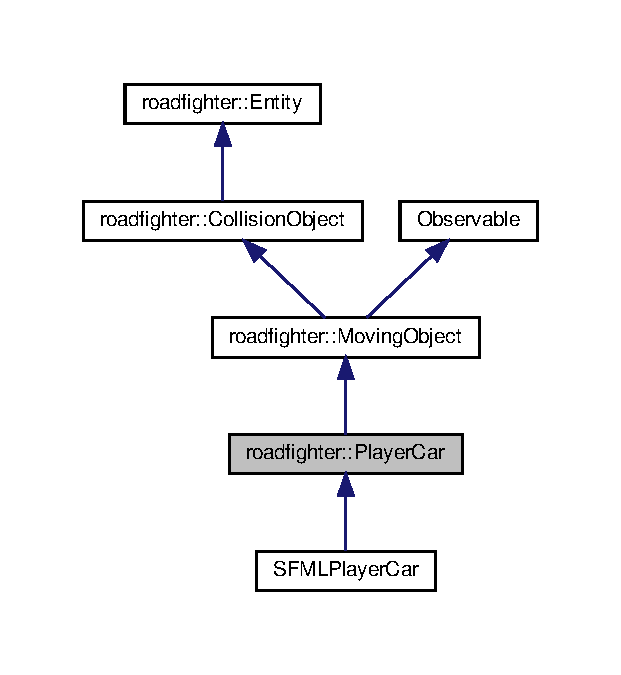
\includegraphics[width=298pt]{classroadfighter_1_1PlayerCar__inherit__graph}
\end{center}
\end{figure}


Collaboration diagram for roadfighter\+:\+:Player\+Car\+:\nopagebreak
\begin{figure}[H]
\begin{center}
\leavevmode
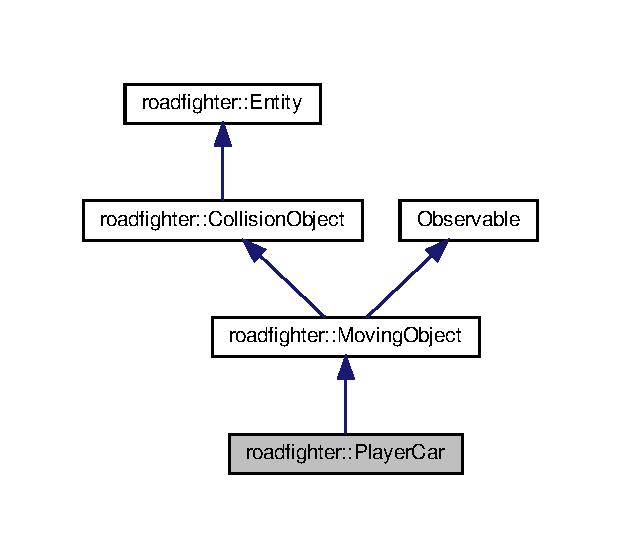
\includegraphics[width=298pt]{classroadfighter_1_1PlayerCar__coll__graph}
\end{center}
\end{figure}
\subsection*{Public Member Functions}
\begin{DoxyCompactItemize}
\item 
\hyperlink{classroadfighter_1_1PlayerCar_ada20f509f074df30613ecfe09e80c79e}{Player\+Car} ()=default
\item 
\hyperlink{classroadfighter_1_1PlayerCar_a0e4db8cf7fc38214fa0383e1518ab2a2}{Player\+Car} (double m\+\_\+max\+Vert\+Speed, double m\+\_\+vert\+Accel, double m\+\_\+hor\+Accel, std\+::shared\+\_\+ptr$<$ \hyperlink{classroadfighter_1_1InputController}{Input\+Controller} $>$ controller, int fuel=100)
\item 
\hyperlink{classroadfighter_1_1PlayerCar_a89f593714201e6d8252abd19125c7c88}{Player\+Car} (const \hyperlink{classroadfighter_1_1PlayerCar}{Player\+Car} \&copy)=default
\item 
\hyperlink{classroadfighter_1_1PlayerCar_a1243a4b2ec289c99884cb1c5f8a57531}{Player\+Car} (\hyperlink{classroadfighter_1_1PlayerCar}{Player\+Car} \&\&move)=default
\item 
\mbox{\Hypertarget{classroadfighter_1_1PlayerCar_a50481f68beb27eeb71c3ecb7ea5bf4a1}\label{classroadfighter_1_1PlayerCar_a50481f68beb27eeb71c3ecb7ea5bf4a1}} 
{\bfseries Player\+Car} (const \hyperlink{classroadfighter_1_1Location}{Location} \&m\+\_\+loc1, const \hyperlink{classroadfighter_1_1Location}{Location} \&m\+\_\+loc2, double m\+\_\+max\+Vert\+Speed, double m\+\_\+vert\+Accel, double m\+\_\+hor\+Accel, double m\+\_\+fuel, const std\+::shared\+\_\+ptr$<$ \hyperlink{classroadfighter_1_1InputController}{Input\+Controller} $>$ \&m\+\_\+move\+Controller, const std\+::shared\+\_\+ptr$<$ \hyperlink{classroadfighter_1_1EntityTransporter}{Entity\+Transporter} $>$ \&transporter, const std\+::shared\+\_\+ptr$<$ \hyperlink{classroadfighter_1_1Entity__Factory__base}{Entity\+\_\+\+Factory\+\_\+base} $>$ \&factory)
\item 
\hyperlink{classroadfighter_1_1PlayerCar}{Player\+Car} \& \hyperlink{classroadfighter_1_1PlayerCar_a1913e3231449aa67ad450ac15267086b}{operator=} (const \hyperlink{classroadfighter_1_1PlayerCar}{Player\+Car} \&other)=default
\item 
\hyperlink{classroadfighter_1_1PlayerCar}{Player\+Car} \& \hyperlink{classroadfighter_1_1PlayerCar_aa6938d2531fea4938eb0837fb2763304}{operator=} (\hyperlink{classroadfighter_1_1PlayerCar}{Player\+Car} \&\&other)=default
\item 
\hyperlink{classroadfighter_1_1PlayerCar_a7da4510fe32e4380f7a5771849ac082c}{$\sim$\+Player\+Car} () override=default
\item 
void \hyperlink{classroadfighter_1_1PlayerCar_a3e0ac4c28d1635e5d142c81beeec05dc}{decreas\+Fuel} (const double \&amount)
\item 
void \hyperlink{classroadfighter_1_1PlayerCar_ac313f0e4a46a6aa155936d3d8154ec4a}{increase\+Fuel} (const double \&amount)
\item 
void \hyperlink{classroadfighter_1_1PlayerCar_aa1dcbec01dde1b212e4919b61338edde}{update\+Movement} (double dt) override
\item 
void \hyperlink{classroadfighter_1_1PlayerCar_a01480487ca7978a50a3c6609f1ebe6df}{update\+Logic} () override
\item 
bool \hyperlink{classroadfighter_1_1PlayerCar_aaf4dc181a4d21e544aecd7a8e538cfd6}{must\+Delete} () const override
\item 
void \hyperlink{classroadfighter_1_1PlayerCar_a12f0da24565a4fe64a7bf17fc7c37152}{win} () override
\item 
void \hyperlink{classroadfighter_1_1PlayerCar_ab62e40d949ac12f402fdaaab15c69b81}{collide\+With} (std\+::shared\+\_\+ptr$<$ \hyperlink{classroadfighter_1_1CollisionObject}{Collision\+Object} $>$ \&collided) override
\item 
void \hyperlink{classroadfighter_1_1PlayerCar_a330d071af729d7afbfcfd7ef92516544}{crash} () override
\item 
void \hyperlink{classroadfighter_1_1PlayerCar_a592556a1c6326c9d9a70691f036eaafc}{shot} () override
\item 
void \hyperlink{classroadfighter_1_1PlayerCar_a0f0626a6ea7d25e3ba01a8289d54acac}{bonus} () override
\item 
double \hyperlink{classroadfighter_1_1PlayerCar_aefc7f96fae66baecef10861a6b1fa0f2}{get\+Fuel} () const
\item 
\mbox{\Hypertarget{classroadfighter_1_1PlayerCar_a65725265e5af175119a4c87be9a74cfe}\label{classroadfighter_1_1PlayerCar_a65725265e5af175119a4c87be9a74cfe}} 
void {\bfseries decreasefire\+Countdown} ()
\item 
\mbox{\Hypertarget{classroadfighter_1_1PlayerCar_a2fdc34f0a8256d3fa8e36378c3c64b10}\label{classroadfighter_1_1PlayerCar_a2fdc34f0a8256d3fa8e36378c3c64b10}} 
void {\bfseries shoot} ()
\end{DoxyCompactItemize}


\subsection{Constructor \& Destructor Documentation}
\mbox{\Hypertarget{classroadfighter_1_1PlayerCar_ada20f509f074df30613ecfe09e80c79e}\label{classroadfighter_1_1PlayerCar_ada20f509f074df30613ecfe09e80c79e}} 
\index{roadfighter\+::\+Player\+Car@{roadfighter\+::\+Player\+Car}!Player\+Car@{Player\+Car}}
\index{Player\+Car@{Player\+Car}!roadfighter\+::\+Player\+Car@{roadfighter\+::\+Player\+Car}}
\subsubsection{\texorpdfstring{Player\+Car()}{PlayerCar()}\hspace{0.1cm}{\footnotesize\ttfamily [1/4]}}
{\footnotesize\ttfamily roadfighter\+::\+Player\+Car\+::\+Player\+Car (\begin{DoxyParamCaption}{ }\end{DoxyParamCaption})\hspace{0.3cm}{\ttfamily [default]}}

default constructor for \hyperlink{classroadfighter_1_1PlayerCar}{Player\+Car} \mbox{\Hypertarget{classroadfighter_1_1PlayerCar_a0e4db8cf7fc38214fa0383e1518ab2a2}\label{classroadfighter_1_1PlayerCar_a0e4db8cf7fc38214fa0383e1518ab2a2}} 
\index{roadfighter\+::\+Player\+Car@{roadfighter\+::\+Player\+Car}!Player\+Car@{Player\+Car}}
\index{Player\+Car@{Player\+Car}!roadfighter\+::\+Player\+Car@{roadfighter\+::\+Player\+Car}}
\subsubsection{\texorpdfstring{Player\+Car()}{PlayerCar()}\hspace{0.1cm}{\footnotesize\ttfamily [2/4]}}
{\footnotesize\ttfamily roadfighter\+::\+Player\+Car\+::\+Player\+Car (\begin{DoxyParamCaption}\item[{double}]{m\+\_\+max\+Vert\+Speed,  }\item[{double}]{m\+\_\+vert\+Accel,  }\item[{double}]{m\+\_\+hor\+Accel,  }\item[{std\+::shared\+\_\+ptr$<$ \hyperlink{classroadfighter_1_1InputController}{Input\+Controller} $>$}]{controller,  }\item[{int}]{fuel = {\ttfamily 100} }\end{DoxyParamCaption})}

constructor with arguments for player\+Car 
\begin{DoxyParams}{Parameters}
{\em controller} & a shared pointer to the move controller the car will use \\
\hline
{\em fuel} & the amount of fuel the car will use (default at 100) \\
\hline
\end{DoxyParams}
\mbox{\Hypertarget{classroadfighter_1_1PlayerCar_a89f593714201e6d8252abd19125c7c88}\label{classroadfighter_1_1PlayerCar_a89f593714201e6d8252abd19125c7c88}} 
\index{roadfighter\+::\+Player\+Car@{roadfighter\+::\+Player\+Car}!Player\+Car@{Player\+Car}}
\index{Player\+Car@{Player\+Car}!roadfighter\+::\+Player\+Car@{roadfighter\+::\+Player\+Car}}
\subsubsection{\texorpdfstring{Player\+Car()}{PlayerCar()}\hspace{0.1cm}{\footnotesize\ttfamily [3/4]}}
{\footnotesize\ttfamily roadfighter\+::\+Player\+Car\+::\+Player\+Car (\begin{DoxyParamCaption}\item[{const \hyperlink{classroadfighter_1_1PlayerCar}{Player\+Car} \&}]{copy }\end{DoxyParamCaption})\hspace{0.3cm}{\ttfamily [default]}}

copy constructor 
\begin{DoxyParams}{Parameters}
{\em copy} & the other \hyperlink{classroadfighter_1_1PlayerCar}{Player\+Car} that is being copied \\
\hline
\end{DoxyParams}
\mbox{\Hypertarget{classroadfighter_1_1PlayerCar_a1243a4b2ec289c99884cb1c5f8a57531}\label{classroadfighter_1_1PlayerCar_a1243a4b2ec289c99884cb1c5f8a57531}} 
\index{roadfighter\+::\+Player\+Car@{roadfighter\+::\+Player\+Car}!Player\+Car@{Player\+Car}}
\index{Player\+Car@{Player\+Car}!roadfighter\+::\+Player\+Car@{roadfighter\+::\+Player\+Car}}
\subsubsection{\texorpdfstring{Player\+Car()}{PlayerCar()}\hspace{0.1cm}{\footnotesize\ttfamily [4/4]}}
{\footnotesize\ttfamily roadfighter\+::\+Player\+Car\+::\+Player\+Car (\begin{DoxyParamCaption}\item[{\hyperlink{classroadfighter_1_1PlayerCar}{Player\+Car} \&\&}]{move }\end{DoxyParamCaption})\hspace{0.3cm}{\ttfamily [default]}}

move constructor 
\begin{DoxyParams}{Parameters}
{\em Move} & the other \hyperlink{classroadfighter_1_1PlayerCar}{Player\+Car} that is being moved in this one \\
\hline
\end{DoxyParams}
\mbox{\Hypertarget{classroadfighter_1_1PlayerCar_a7da4510fe32e4380f7a5771849ac082c}\label{classroadfighter_1_1PlayerCar_a7da4510fe32e4380f7a5771849ac082c}} 
\index{roadfighter\+::\+Player\+Car@{roadfighter\+::\+Player\+Car}!````~Player\+Car@{$\sim$\+Player\+Car}}
\index{````~Player\+Car@{$\sim$\+Player\+Car}!roadfighter\+::\+Player\+Car@{roadfighter\+::\+Player\+Car}}
\subsubsection{\texorpdfstring{$\sim$\+Player\+Car()}{~PlayerCar()}}
{\footnotesize\ttfamily roadfighter\+::\+Player\+Car\+::$\sim$\+Player\+Car (\begin{DoxyParamCaption}{ }\end{DoxyParamCaption})\hspace{0.3cm}{\ttfamily [override]}, {\ttfamily [default]}}

destructor for \hyperlink{classroadfighter_1_1PlayerCar}{Player\+Car} 

\subsection{Member Function Documentation}
\mbox{\Hypertarget{classroadfighter_1_1PlayerCar_a0f0626a6ea7d25e3ba01a8289d54acac}\label{classroadfighter_1_1PlayerCar_a0f0626a6ea7d25e3ba01a8289d54acac}} 
\index{roadfighter\+::\+Player\+Car@{roadfighter\+::\+Player\+Car}!bonus@{bonus}}
\index{bonus@{bonus}!roadfighter\+::\+Player\+Car@{roadfighter\+::\+Player\+Car}}
\subsubsection{\texorpdfstring{bonus()}{bonus()}}
{\footnotesize\ttfamily void roadfighter\+::\+Player\+Car\+::bonus (\begin{DoxyParamCaption}{ }\end{DoxyParamCaption})\hspace{0.3cm}{\ttfamily [override]}, {\ttfamily [virtual]}}

this function says what will happen if the car gets a bonus 

Implements \hyperlink{classroadfighter_1_1CollisionObject_a157e499c27619ceefd6179a459fafd90}{roadfighter\+::\+Collision\+Object}.

\mbox{\Hypertarget{classroadfighter_1_1PlayerCar_ab62e40d949ac12f402fdaaab15c69b81}\label{classroadfighter_1_1PlayerCar_ab62e40d949ac12f402fdaaab15c69b81}} 
\index{roadfighter\+::\+Player\+Car@{roadfighter\+::\+Player\+Car}!collide\+With@{collide\+With}}
\index{collide\+With@{collide\+With}!roadfighter\+::\+Player\+Car@{roadfighter\+::\+Player\+Car}}
\subsubsection{\texorpdfstring{collide\+With()}{collideWith()}}
{\footnotesize\ttfamily void roadfighter\+::\+Player\+Car\+::collide\+With (\begin{DoxyParamCaption}\item[{std\+::shared\+\_\+ptr$<$ \hyperlink{classroadfighter_1_1CollisionObject}{Collision\+Object} $>$ \&}]{collided }\end{DoxyParamCaption})\hspace{0.3cm}{\ttfamily [override]}, {\ttfamily [virtual]}}

this function will handle the logic about what will happen if another object crashes into it 
\begin{DoxyParams}{Parameters}
{\em collided} & the object that crashes into the playercar \\
\hline
\end{DoxyParams}


Implements \hyperlink{classroadfighter_1_1CollisionObject_a7eafa2fdc4463788b816fdd9370d28d9}{roadfighter\+::\+Collision\+Object}.

\mbox{\Hypertarget{classroadfighter_1_1PlayerCar_a330d071af729d7afbfcfd7ef92516544}\label{classroadfighter_1_1PlayerCar_a330d071af729d7afbfcfd7ef92516544}} 
\index{roadfighter\+::\+Player\+Car@{roadfighter\+::\+Player\+Car}!crash@{crash}}
\index{crash@{crash}!roadfighter\+::\+Player\+Car@{roadfighter\+::\+Player\+Car}}
\subsubsection{\texorpdfstring{crash()}{crash()}}
{\footnotesize\ttfamily void roadfighter\+::\+Player\+Car\+::crash (\begin{DoxyParamCaption}{ }\end{DoxyParamCaption})\hspace{0.3cm}{\ttfamily [override]}, {\ttfamily [virtual]}}

this function says what will happen if the car crashes 

Implements \hyperlink{classroadfighter_1_1CollisionObject_a18f0f60a5a664d6fb554daac0d398a2c}{roadfighter\+::\+Collision\+Object}.

\mbox{\Hypertarget{classroadfighter_1_1PlayerCar_a3e0ac4c28d1635e5d142c81beeec05dc}\label{classroadfighter_1_1PlayerCar_a3e0ac4c28d1635e5d142c81beeec05dc}} 
\index{roadfighter\+::\+Player\+Car@{roadfighter\+::\+Player\+Car}!decreas\+Fuel@{decreas\+Fuel}}
\index{decreas\+Fuel@{decreas\+Fuel}!roadfighter\+::\+Player\+Car@{roadfighter\+::\+Player\+Car}}
\subsubsection{\texorpdfstring{decreas\+Fuel()}{decreasFuel()}}
{\footnotesize\ttfamily void roadfighter\+::\+Player\+Car\+::decreas\+Fuel (\begin{DoxyParamCaption}\item[{const double \&}]{amount }\end{DoxyParamCaption})}

this function decreases the fuel by the given amount 
\begin{DoxyParams}{Parameters}
{\em amount} & \\
\hline
\end{DoxyParams}
\mbox{\Hypertarget{classroadfighter_1_1PlayerCar_aefc7f96fae66baecef10861a6b1fa0f2}\label{classroadfighter_1_1PlayerCar_aefc7f96fae66baecef10861a6b1fa0f2}} 
\index{roadfighter\+::\+Player\+Car@{roadfighter\+::\+Player\+Car}!get\+Fuel@{get\+Fuel}}
\index{get\+Fuel@{get\+Fuel}!roadfighter\+::\+Player\+Car@{roadfighter\+::\+Player\+Car}}
\subsubsection{\texorpdfstring{get\+Fuel()}{getFuel()}}
{\footnotesize\ttfamily double roadfighter\+::\+Player\+Car\+::get\+Fuel (\begin{DoxyParamCaption}{ }\end{DoxyParamCaption}) const}

getter for the fual of the car \begin{DoxyReturn}{Returns}
a double depicting the fuel 
\end{DoxyReturn}
\mbox{\Hypertarget{classroadfighter_1_1PlayerCar_ac313f0e4a46a6aa155936d3d8154ec4a}\label{classroadfighter_1_1PlayerCar_ac313f0e4a46a6aa155936d3d8154ec4a}} 
\index{roadfighter\+::\+Player\+Car@{roadfighter\+::\+Player\+Car}!increase\+Fuel@{increase\+Fuel}}
\index{increase\+Fuel@{increase\+Fuel}!roadfighter\+::\+Player\+Car@{roadfighter\+::\+Player\+Car}}
\subsubsection{\texorpdfstring{increase\+Fuel()}{increaseFuel()}}
{\footnotesize\ttfamily void roadfighter\+::\+Player\+Car\+::increase\+Fuel (\begin{DoxyParamCaption}\item[{const double \&}]{amount }\end{DoxyParamCaption})}

this function increases the fuel by the given amount 
\begin{DoxyParams}{Parameters}
{\em amount} & \\
\hline
\end{DoxyParams}
\mbox{\Hypertarget{classroadfighter_1_1PlayerCar_aaf4dc181a4d21e544aecd7a8e538cfd6}\label{classroadfighter_1_1PlayerCar_aaf4dc181a4d21e544aecd7a8e538cfd6}} 
\index{roadfighter\+::\+Player\+Car@{roadfighter\+::\+Player\+Car}!must\+Delete@{must\+Delete}}
\index{must\+Delete@{must\+Delete}!roadfighter\+::\+Player\+Car@{roadfighter\+::\+Player\+Car}}
\subsubsection{\texorpdfstring{must\+Delete()}{mustDelete()}}
{\footnotesize\ttfamily bool roadfighter\+::\+Player\+Car\+::must\+Delete (\begin{DoxyParamCaption}{ }\end{DoxyParamCaption}) const\hspace{0.3cm}{\ttfamily [override]}, {\ttfamily [virtual]}}

this function well say wether the car can be deletet or not \begin{DoxyReturn}{Returns}
playercar can never be deletet so it will always be false 
\end{DoxyReturn}


Reimplemented from \hyperlink{classroadfighter_1_1CollisionObject_a738071cd7b1b8cd4c8d455b5e552bd4c}{roadfighter\+::\+Collision\+Object}.

\mbox{\Hypertarget{classroadfighter_1_1PlayerCar_a1913e3231449aa67ad450ac15267086b}\label{classroadfighter_1_1PlayerCar_a1913e3231449aa67ad450ac15267086b}} 
\index{roadfighter\+::\+Player\+Car@{roadfighter\+::\+Player\+Car}!operator=@{operator=}}
\index{operator=@{operator=}!roadfighter\+::\+Player\+Car@{roadfighter\+::\+Player\+Car}}
\subsubsection{\texorpdfstring{operator=()}{operator=()}\hspace{0.1cm}{\footnotesize\ttfamily [1/2]}}
{\footnotesize\ttfamily \hyperlink{classroadfighter_1_1PlayerCar}{Player\+Car}\& roadfighter\+::\+Player\+Car\+::operator= (\begin{DoxyParamCaption}\item[{const \hyperlink{classroadfighter_1_1PlayerCar}{Player\+Car} \&}]{other }\end{DoxyParamCaption})\hspace{0.3cm}{\ttfamily [default]}}

copy assigment for \hyperlink{classroadfighter_1_1PlayerCar}{Player\+Car} 
\begin{DoxyParams}{Parameters}
{\em other} & the \hyperlink{classroadfighter_1_1PlayerCar}{Player\+Car} that is being copied \\
\hline
\end{DoxyParams}
\begin{DoxyReturn}{Returns}
a new \hyperlink{classroadfighter_1_1PlayerCar}{Player\+Car} that is equal to the other one 
\end{DoxyReturn}
\mbox{\Hypertarget{classroadfighter_1_1PlayerCar_aa6938d2531fea4938eb0837fb2763304}\label{classroadfighter_1_1PlayerCar_aa6938d2531fea4938eb0837fb2763304}} 
\index{roadfighter\+::\+Player\+Car@{roadfighter\+::\+Player\+Car}!operator=@{operator=}}
\index{operator=@{operator=}!roadfighter\+::\+Player\+Car@{roadfighter\+::\+Player\+Car}}
\subsubsection{\texorpdfstring{operator=()}{operator=()}\hspace{0.1cm}{\footnotesize\ttfamily [2/2]}}
{\footnotesize\ttfamily \hyperlink{classroadfighter_1_1PlayerCar}{Player\+Car}\& roadfighter\+::\+Player\+Car\+::operator= (\begin{DoxyParamCaption}\item[{\hyperlink{classroadfighter_1_1PlayerCar}{Player\+Car} \&\&}]{other }\end{DoxyParamCaption})\hspace{0.3cm}{\ttfamily [default]}}

move assignment for \hyperlink{classroadfighter_1_1PlayerCar}{Player\+Car} 
\begin{DoxyParams}{Parameters}
{\em other} & other \hyperlink{classroadfighter_1_1PlayerCar}{Player\+Car} that is being moved \\
\hline
\end{DoxyParams}
\begin{DoxyReturn}{Returns}
a \hyperlink{classroadfighter_1_1PlayerCar}{Player\+Car} that contains all the data of the first one 
\end{DoxyReturn}
\mbox{\Hypertarget{classroadfighter_1_1PlayerCar_a592556a1c6326c9d9a70691f036eaafc}\label{classroadfighter_1_1PlayerCar_a592556a1c6326c9d9a70691f036eaafc}} 
\index{roadfighter\+::\+Player\+Car@{roadfighter\+::\+Player\+Car}!shot@{shot}}
\index{shot@{shot}!roadfighter\+::\+Player\+Car@{roadfighter\+::\+Player\+Car}}
\subsubsection{\texorpdfstring{shot()}{shot()}}
{\footnotesize\ttfamily void roadfighter\+::\+Player\+Car\+::shot (\begin{DoxyParamCaption}{ }\end{DoxyParamCaption})\hspace{0.3cm}{\ttfamily [override]}, {\ttfamily [virtual]}}

this function says what will happen if the car gets shot 

Implements \hyperlink{classroadfighter_1_1CollisionObject_a338a1071e6d5e25439e57c8673308dbb}{roadfighter\+::\+Collision\+Object}.

\mbox{\Hypertarget{classroadfighter_1_1PlayerCar_a01480487ca7978a50a3c6609f1ebe6df}\label{classroadfighter_1_1PlayerCar_a01480487ca7978a50a3c6609f1ebe6df}} 
\index{roadfighter\+::\+Player\+Car@{roadfighter\+::\+Player\+Car}!update\+Logic@{update\+Logic}}
\index{update\+Logic@{update\+Logic}!roadfighter\+::\+Player\+Car@{roadfighter\+::\+Player\+Car}}
\subsubsection{\texorpdfstring{update\+Logic()}{updateLogic()}}
{\footnotesize\ttfamily void roadfighter\+::\+Player\+Car\+::update\+Logic (\begin{DoxyParamCaption}{ }\end{DoxyParamCaption})\hspace{0.3cm}{\ttfamily [override]}, {\ttfamily [virtual]}}

this funtion updates the logic of the player car 

Reimplemented from \hyperlink{classroadfighter_1_1MovingObject_a2c5d69054a59fc5c6d7458f864ee9d57}{roadfighter\+::\+Moving\+Object}.

\mbox{\Hypertarget{classroadfighter_1_1PlayerCar_aa1dcbec01dde1b212e4919b61338edde}\label{classroadfighter_1_1PlayerCar_aa1dcbec01dde1b212e4919b61338edde}} 
\index{roadfighter\+::\+Player\+Car@{roadfighter\+::\+Player\+Car}!update\+Movement@{update\+Movement}}
\index{update\+Movement@{update\+Movement}!roadfighter\+::\+Player\+Car@{roadfighter\+::\+Player\+Car}}
\subsubsection{\texorpdfstring{update\+Movement()}{updateMovement()}}
{\footnotesize\ttfamily void roadfighter\+::\+Player\+Car\+::update\+Movement (\begin{DoxyParamCaption}\item[{double}]{dt }\end{DoxyParamCaption})\hspace{0.3cm}{\ttfamily [override]}, {\ttfamily [virtual]}}

this function updates the movement by dt ticks, it is also capable of changing the direction 
\begin{DoxyParams}{Parameters}
{\em dt} & the amount of a tick the car will move forward \\
\hline
\end{DoxyParams}


Reimplemented from \hyperlink{classroadfighter_1_1MovingObject_ac1918d96dac118c4bd7d99168d92867c}{roadfighter\+::\+Moving\+Object}.

\mbox{\Hypertarget{classroadfighter_1_1PlayerCar_a12f0da24565a4fe64a7bf17fc7c37152}\label{classroadfighter_1_1PlayerCar_a12f0da24565a4fe64a7bf17fc7c37152}} 
\index{roadfighter\+::\+Player\+Car@{roadfighter\+::\+Player\+Car}!win@{win}}
\index{win@{win}!roadfighter\+::\+Player\+Car@{roadfighter\+::\+Player\+Car}}
\subsubsection{\texorpdfstring{win()}{win()}}
{\footnotesize\ttfamily void roadfighter\+::\+Player\+Car\+::win (\begin{DoxyParamCaption}{ }\end{DoxyParamCaption})\hspace{0.3cm}{\ttfamily [override]}, {\ttfamily [virtual]}}

this function says what the car will do when it wins 

Implements \hyperlink{classroadfighter_1_1CollisionObject_a03ce1ae52676088839d85c597743052c}{roadfighter\+::\+Collision\+Object}.



The documentation for this class was generated from the following files\+:\begin{DoxyCompactItemize}
\item 
Game\+Logic/include/\+Entities/Player\+Car.\+h\item 
Game\+Logic/\+Source/\+Entities/Player\+Car.\+cpp\end{DoxyCompactItemize}

\hypertarget{classroadfighter_1_1RacingCar}{}\section{roadfighter\+:\+:Racing\+Car Class Reference}
\label{classroadfighter_1_1RacingCar}\index{roadfighter\+::\+Racing\+Car@{roadfighter\+::\+Racing\+Car}}


Inheritance diagram for roadfighter\+:\+:Racing\+Car\+:\nopagebreak
\begin{figure}[H]
\begin{center}
\leavevmode
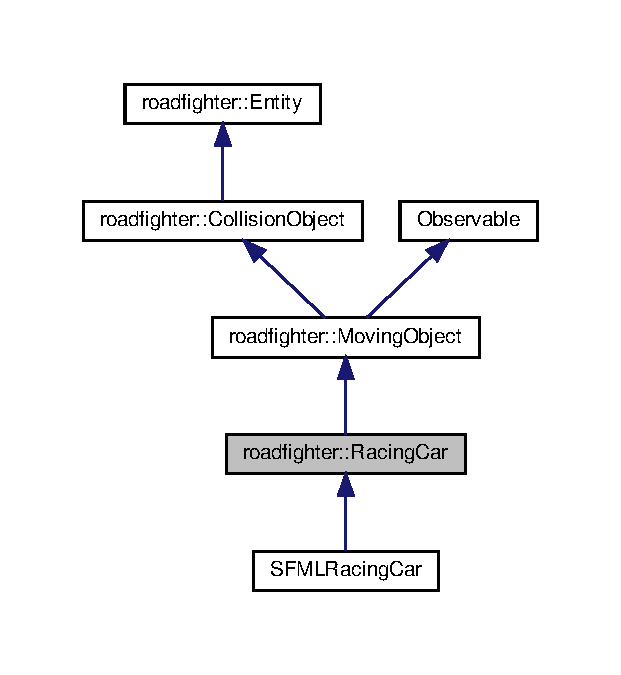
\includegraphics[width=298pt]{classroadfighter_1_1RacingCar__inherit__graph}
\end{center}
\end{figure}


Collaboration diagram for roadfighter\+:\+:Racing\+Car\+:\nopagebreak
\begin{figure}[H]
\begin{center}
\leavevmode
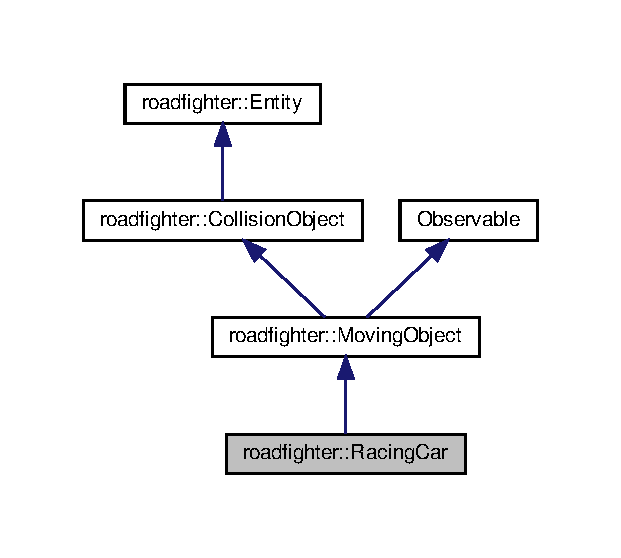
\includegraphics[width=298pt]{classroadfighter_1_1RacingCar__coll__graph}
\end{center}
\end{figure}
\subsection*{Public Member Functions}
\begin{DoxyCompactItemize}
\item 
\hyperlink{classroadfighter_1_1RacingCar_ad36c66bdc36a849289d42b5061be2572}{Racing\+Car} ()=default
\item 
\hyperlink{classroadfighter_1_1RacingCar_ad69732f995ae7a2ee44315cd6a3fc69a}{Racing\+Car} (const \hyperlink{classroadfighter_1_1RacingCar}{Racing\+Car} \&copy)=default
\item 
\hyperlink{classroadfighter_1_1RacingCar_aacfc42aa87c6b5db3f4b80f8fbc68c74}{Racing\+Car} (\hyperlink{classroadfighter_1_1RacingCar}{Racing\+Car} \&\&move)=default
\item 
\mbox{\Hypertarget{classroadfighter_1_1RacingCar_a10f2b7ee84e6859a72bccf1b922fc7f2}\label{classroadfighter_1_1RacingCar_a10f2b7ee84e6859a72bccf1b922fc7f2}} 
{\bfseries Racing\+Car} (const \hyperlink{classroadfighter_1_1Location}{Location} \&m\+\_\+loc1, const \hyperlink{classroadfighter_1_1Location}{Location} \&m\+\_\+loc2, double m\+\_\+max\+Vert\+Speed, double m\+\_\+vert\+Accel, double m\+\_\+hor\+Accel)
\item 
\hyperlink{classroadfighter_1_1RacingCar}{Racing\+Car} \& \hyperlink{classroadfighter_1_1RacingCar_a2df3fdffc4c55aa85a6d9265913aa7b0}{operator=} (const \hyperlink{classroadfighter_1_1RacingCar}{Racing\+Car} \&other)=default
\item 
\hyperlink{classroadfighter_1_1RacingCar}{Racing\+Car} \& \hyperlink{classroadfighter_1_1RacingCar_a370fa9acf725d13ecb5b96ccce61b9d3}{operator=} (\hyperlink{classroadfighter_1_1RacingCar}{Racing\+Car} \&\&other)=default
\item 
\hyperlink{classroadfighter_1_1RacingCar_a1ae41bc99dca96cde8187f4ba2172ea7}{$\sim$\+Racing\+Car} () override=default
\item 
void \hyperlink{classroadfighter_1_1RacingCar_a2e8f3c63381a1fe432cddcc1f34fb935}{update\+Movement} (double dt) override
\item 
void \hyperlink{classroadfighter_1_1RacingCar_af3f3b4c368ba61c13dc9b99004895c5d}{update\+Logic} () override
\item 
bool \hyperlink{classroadfighter_1_1RacingCar_a300bccb330cc8e84834edd5f85354a10}{must\+Delete} () const override
\item 
void \hyperlink{classroadfighter_1_1RacingCar_a24293ac56920da01d29fe99aee8d3ea6}{win} () override
\item 
void \hyperlink{classroadfighter_1_1RacingCar_a1de00cf7c8df548e8ab57a27cefb7345}{collide\+With} (std\+::shared\+\_\+ptr$<$ \hyperlink{classroadfighter_1_1CollisionObject}{Collision\+Object} $>$ \&collided) override
\item 
void \hyperlink{classroadfighter_1_1RacingCar_a2f5018f17852d75682afd78e806b8e4c}{crash} () override
\item 
void \hyperlink{classroadfighter_1_1RacingCar_a20c4363a1d31cc17d7d82c8f9a219d2d}{shot} () override
\item 
void \hyperlink{classroadfighter_1_1RacingCar_a5858dd3f2c7bb49782b29c0a90846a6c}{bonus} () override
\end{DoxyCompactItemize}


\subsection{Constructor \& Destructor Documentation}
\mbox{\Hypertarget{classroadfighter_1_1RacingCar_ad36c66bdc36a849289d42b5061be2572}\label{classroadfighter_1_1RacingCar_ad36c66bdc36a849289d42b5061be2572}} 
\index{roadfighter\+::\+Racing\+Car@{roadfighter\+::\+Racing\+Car}!Racing\+Car@{Racing\+Car}}
\index{Racing\+Car@{Racing\+Car}!roadfighter\+::\+Racing\+Car@{roadfighter\+::\+Racing\+Car}}
\subsubsection{\texorpdfstring{Racing\+Car()}{RacingCar()}\hspace{0.1cm}{\footnotesize\ttfamily [1/3]}}
{\footnotesize\ttfamily roadfighter\+::\+Racing\+Car\+::\+Racing\+Car (\begin{DoxyParamCaption}{ }\end{DoxyParamCaption})\hspace{0.3cm}{\ttfamily [default]}}

default constructor for \hyperlink{classroadfighter_1_1RacingCar}{Racing\+Car} \mbox{\Hypertarget{classroadfighter_1_1RacingCar_ad69732f995ae7a2ee44315cd6a3fc69a}\label{classroadfighter_1_1RacingCar_ad69732f995ae7a2ee44315cd6a3fc69a}} 
\index{roadfighter\+::\+Racing\+Car@{roadfighter\+::\+Racing\+Car}!Racing\+Car@{Racing\+Car}}
\index{Racing\+Car@{Racing\+Car}!roadfighter\+::\+Racing\+Car@{roadfighter\+::\+Racing\+Car}}
\subsubsection{\texorpdfstring{Racing\+Car()}{RacingCar()}\hspace{0.1cm}{\footnotesize\ttfamily [2/3]}}
{\footnotesize\ttfamily roadfighter\+::\+Racing\+Car\+::\+Racing\+Car (\begin{DoxyParamCaption}\item[{const \hyperlink{classroadfighter_1_1RacingCar}{Racing\+Car} \&}]{copy }\end{DoxyParamCaption})\hspace{0.3cm}{\ttfamily [default]}}

copy constructor 
\begin{DoxyParams}{Parameters}
{\em copy} & the other \hyperlink{classroadfighter_1_1RacingCar}{Racing\+Car} that is being copied \\
\hline
\end{DoxyParams}
\mbox{\Hypertarget{classroadfighter_1_1RacingCar_aacfc42aa87c6b5db3f4b80f8fbc68c74}\label{classroadfighter_1_1RacingCar_aacfc42aa87c6b5db3f4b80f8fbc68c74}} 
\index{roadfighter\+::\+Racing\+Car@{roadfighter\+::\+Racing\+Car}!Racing\+Car@{Racing\+Car}}
\index{Racing\+Car@{Racing\+Car}!roadfighter\+::\+Racing\+Car@{roadfighter\+::\+Racing\+Car}}
\subsubsection{\texorpdfstring{Racing\+Car()}{RacingCar()}\hspace{0.1cm}{\footnotesize\ttfamily [3/3]}}
{\footnotesize\ttfamily roadfighter\+::\+Racing\+Car\+::\+Racing\+Car (\begin{DoxyParamCaption}\item[{\hyperlink{classroadfighter_1_1RacingCar}{Racing\+Car} \&\&}]{move }\end{DoxyParamCaption})\hspace{0.3cm}{\ttfamily [default]}}

move constructor 
\begin{DoxyParams}{Parameters}
{\em Move} & the other \hyperlink{classroadfighter_1_1RacingCar}{Racing\+Car} that is being moved in this one \\
\hline
\end{DoxyParams}
\mbox{\Hypertarget{classroadfighter_1_1RacingCar_a1ae41bc99dca96cde8187f4ba2172ea7}\label{classroadfighter_1_1RacingCar_a1ae41bc99dca96cde8187f4ba2172ea7}} 
\index{roadfighter\+::\+Racing\+Car@{roadfighter\+::\+Racing\+Car}!````~Racing\+Car@{$\sim$\+Racing\+Car}}
\index{````~Racing\+Car@{$\sim$\+Racing\+Car}!roadfighter\+::\+Racing\+Car@{roadfighter\+::\+Racing\+Car}}
\subsubsection{\texorpdfstring{$\sim$\+Racing\+Car()}{~RacingCar()}}
{\footnotesize\ttfamily roadfighter\+::\+Racing\+Car\+::$\sim$\+Racing\+Car (\begin{DoxyParamCaption}{ }\end{DoxyParamCaption})\hspace{0.3cm}{\ttfamily [override]}, {\ttfamily [default]}}

destructor for \hyperlink{classroadfighter_1_1RacingCar}{Racing\+Car} 

\subsection{Member Function Documentation}
\mbox{\Hypertarget{classroadfighter_1_1RacingCar_a5858dd3f2c7bb49782b29c0a90846a6c}\label{classroadfighter_1_1RacingCar_a5858dd3f2c7bb49782b29c0a90846a6c}} 
\index{roadfighter\+::\+Racing\+Car@{roadfighter\+::\+Racing\+Car}!bonus@{bonus}}
\index{bonus@{bonus}!roadfighter\+::\+Racing\+Car@{roadfighter\+::\+Racing\+Car}}
\subsubsection{\texorpdfstring{bonus()}{bonus()}}
{\footnotesize\ttfamily void roadfighter\+::\+Racing\+Car\+::bonus (\begin{DoxyParamCaption}{ }\end{DoxyParamCaption})\hspace{0.3cm}{\ttfamily [override]}, {\ttfamily [virtual]}}

this function will handle what happens when the car gets a bonus 

Implements \hyperlink{classroadfighter_1_1CollisionObject_a157e499c27619ceefd6179a459fafd90}{roadfighter\+::\+Collision\+Object}.

\mbox{\Hypertarget{classroadfighter_1_1RacingCar_a1de00cf7c8df548e8ab57a27cefb7345}\label{classroadfighter_1_1RacingCar_a1de00cf7c8df548e8ab57a27cefb7345}} 
\index{roadfighter\+::\+Racing\+Car@{roadfighter\+::\+Racing\+Car}!collide\+With@{collide\+With}}
\index{collide\+With@{collide\+With}!roadfighter\+::\+Racing\+Car@{roadfighter\+::\+Racing\+Car}}
\subsubsection{\texorpdfstring{collide\+With()}{collideWith()}}
{\footnotesize\ttfamily void roadfighter\+::\+Racing\+Car\+::collide\+With (\begin{DoxyParamCaption}\item[{std\+::shared\+\_\+ptr$<$ \hyperlink{classroadfighter_1_1CollisionObject}{Collision\+Object} $>$ \&}]{collided }\end{DoxyParamCaption})\hspace{0.3cm}{\ttfamily [override]}, {\ttfamily [virtual]}}

this function handles what happens when another object collides with the playercar 
\begin{DoxyParams}{Parameters}
{\em collided} & the object that collides with the playercar \\
\hline
\end{DoxyParams}


Implements \hyperlink{classroadfighter_1_1CollisionObject_a7eafa2fdc4463788b816fdd9370d28d9}{roadfighter\+::\+Collision\+Object}.

\mbox{\Hypertarget{classroadfighter_1_1RacingCar_a2f5018f17852d75682afd78e806b8e4c}\label{classroadfighter_1_1RacingCar_a2f5018f17852d75682afd78e806b8e4c}} 
\index{roadfighter\+::\+Racing\+Car@{roadfighter\+::\+Racing\+Car}!crash@{crash}}
\index{crash@{crash}!roadfighter\+::\+Racing\+Car@{roadfighter\+::\+Racing\+Car}}
\subsubsection{\texorpdfstring{crash()}{crash()}}
{\footnotesize\ttfamily void roadfighter\+::\+Racing\+Car\+::crash (\begin{DoxyParamCaption}{ }\end{DoxyParamCaption})\hspace{0.3cm}{\ttfamily [override]}, {\ttfamily [virtual]}}

this function will handle what happens when the car gets crashes 

Implements \hyperlink{classroadfighter_1_1CollisionObject_a18f0f60a5a664d6fb554daac0d398a2c}{roadfighter\+::\+Collision\+Object}.

\mbox{\Hypertarget{classroadfighter_1_1RacingCar_a300bccb330cc8e84834edd5f85354a10}\label{classroadfighter_1_1RacingCar_a300bccb330cc8e84834edd5f85354a10}} 
\index{roadfighter\+::\+Racing\+Car@{roadfighter\+::\+Racing\+Car}!must\+Delete@{must\+Delete}}
\index{must\+Delete@{must\+Delete}!roadfighter\+::\+Racing\+Car@{roadfighter\+::\+Racing\+Car}}
\subsubsection{\texorpdfstring{must\+Delete()}{mustDelete()}}
{\footnotesize\ttfamily bool roadfighter\+::\+Racing\+Car\+::must\+Delete (\begin{DoxyParamCaption}{ }\end{DoxyParamCaption}) const\hspace{0.3cm}{\ttfamily [override]}, {\ttfamily [virtual]}}

a function that should be overriden and is used to denote wether an object should be deletet or not \begin{DoxyReturn}{Returns}
a bool 
\end{DoxyReturn}


Reimplemented from \hyperlink{classroadfighter_1_1CollisionObject_a738071cd7b1b8cd4c8d455b5e552bd4c}{roadfighter\+::\+Collision\+Object}.

\mbox{\Hypertarget{classroadfighter_1_1RacingCar_a2df3fdffc4c55aa85a6d9265913aa7b0}\label{classroadfighter_1_1RacingCar_a2df3fdffc4c55aa85a6d9265913aa7b0}} 
\index{roadfighter\+::\+Racing\+Car@{roadfighter\+::\+Racing\+Car}!operator=@{operator=}}
\index{operator=@{operator=}!roadfighter\+::\+Racing\+Car@{roadfighter\+::\+Racing\+Car}}
\subsubsection{\texorpdfstring{operator=()}{operator=()}\hspace{0.1cm}{\footnotesize\ttfamily [1/2]}}
{\footnotesize\ttfamily \hyperlink{classroadfighter_1_1RacingCar}{Racing\+Car}\& roadfighter\+::\+Racing\+Car\+::operator= (\begin{DoxyParamCaption}\item[{const \hyperlink{classroadfighter_1_1RacingCar}{Racing\+Car} \&}]{other }\end{DoxyParamCaption})\hspace{0.3cm}{\ttfamily [default]}}

copy assigment for \hyperlink{classroadfighter_1_1RacingCar}{Racing\+Car} 
\begin{DoxyParams}{Parameters}
{\em other} & the \hyperlink{classroadfighter_1_1RacingCar}{Racing\+Car} that is being copied \\
\hline
\end{DoxyParams}
\begin{DoxyReturn}{Returns}
a new \hyperlink{classroadfighter_1_1RacingCar}{Racing\+Car} that is equal to the other one 
\end{DoxyReturn}
\mbox{\Hypertarget{classroadfighter_1_1RacingCar_a370fa9acf725d13ecb5b96ccce61b9d3}\label{classroadfighter_1_1RacingCar_a370fa9acf725d13ecb5b96ccce61b9d3}} 
\index{roadfighter\+::\+Racing\+Car@{roadfighter\+::\+Racing\+Car}!operator=@{operator=}}
\index{operator=@{operator=}!roadfighter\+::\+Racing\+Car@{roadfighter\+::\+Racing\+Car}}
\subsubsection{\texorpdfstring{operator=()}{operator=()}\hspace{0.1cm}{\footnotesize\ttfamily [2/2]}}
{\footnotesize\ttfamily \hyperlink{classroadfighter_1_1RacingCar}{Racing\+Car}\& roadfighter\+::\+Racing\+Car\+::operator= (\begin{DoxyParamCaption}\item[{\hyperlink{classroadfighter_1_1RacingCar}{Racing\+Car} \&\&}]{other }\end{DoxyParamCaption})\hspace{0.3cm}{\ttfamily [default]}}

move assignment for \hyperlink{classroadfighter_1_1RacingCar}{Racing\+Car} 
\begin{DoxyParams}{Parameters}
{\em other} & other \hyperlink{classroadfighter_1_1RacingCar}{Racing\+Car} that is being moved \\
\hline
\end{DoxyParams}
\begin{DoxyReturn}{Returns}
a \hyperlink{classroadfighter_1_1RacingCar}{Racing\+Car} that contains all the data of the first one 
\end{DoxyReturn}
\mbox{\Hypertarget{classroadfighter_1_1RacingCar_a20c4363a1d31cc17d7d82c8f9a219d2d}\label{classroadfighter_1_1RacingCar_a20c4363a1d31cc17d7d82c8f9a219d2d}} 
\index{roadfighter\+::\+Racing\+Car@{roadfighter\+::\+Racing\+Car}!shot@{shot}}
\index{shot@{shot}!roadfighter\+::\+Racing\+Car@{roadfighter\+::\+Racing\+Car}}
\subsubsection{\texorpdfstring{shot()}{shot()}}
{\footnotesize\ttfamily void roadfighter\+::\+Racing\+Car\+::shot (\begin{DoxyParamCaption}{ }\end{DoxyParamCaption})\hspace{0.3cm}{\ttfamily [override]}, {\ttfamily [virtual]}}

this function will handle what happens when the car gets shot 

Implements \hyperlink{classroadfighter_1_1CollisionObject_a338a1071e6d5e25439e57c8673308dbb}{roadfighter\+::\+Collision\+Object}.

\mbox{\Hypertarget{classroadfighter_1_1RacingCar_af3f3b4c368ba61c13dc9b99004895c5d}\label{classroadfighter_1_1RacingCar_af3f3b4c368ba61c13dc9b99004895c5d}} 
\index{roadfighter\+::\+Racing\+Car@{roadfighter\+::\+Racing\+Car}!update\+Logic@{update\+Logic}}
\index{update\+Logic@{update\+Logic}!roadfighter\+::\+Racing\+Car@{roadfighter\+::\+Racing\+Car}}
\subsubsection{\texorpdfstring{update\+Logic()}{updateLogic()}}
{\footnotesize\ttfamily void roadfighter\+::\+Racing\+Car\+::update\+Logic (\begin{DoxyParamCaption}{ }\end{DoxyParamCaption})\hspace{0.3cm}{\ttfamily [override]}, {\ttfamily [virtual]}}

this function will update the logic of the racing car here it also can cahnge the direction 

Reimplemented from \hyperlink{classroadfighter_1_1MovingObject_a2c5d69054a59fc5c6d7458f864ee9d57}{roadfighter\+::\+Moving\+Object}.

\mbox{\Hypertarget{classroadfighter_1_1RacingCar_a2e8f3c63381a1fe432cddcc1f34fb935}\label{classroadfighter_1_1RacingCar_a2e8f3c63381a1fe432cddcc1f34fb935}} 
\index{roadfighter\+::\+Racing\+Car@{roadfighter\+::\+Racing\+Car}!update\+Movement@{update\+Movement}}
\index{update\+Movement@{update\+Movement}!roadfighter\+::\+Racing\+Car@{roadfighter\+::\+Racing\+Car}}
\subsubsection{\texorpdfstring{update\+Movement()}{updateMovement()}}
{\footnotesize\ttfamily void roadfighter\+::\+Racing\+Car\+::update\+Movement (\begin{DoxyParamCaption}\item[{double}]{dt }\end{DoxyParamCaption})\hspace{0.3cm}{\ttfamily [override]}, {\ttfamily [virtual]}}

this function will update the postion of the car by dt ticks 
\begin{DoxyParams}{Parameters}
{\em dt} & the amount of a tick the car will be moved forwar \\
\hline
\end{DoxyParams}


Reimplemented from \hyperlink{classroadfighter_1_1MovingObject_ac1918d96dac118c4bd7d99168d92867c}{roadfighter\+::\+Moving\+Object}.

\mbox{\Hypertarget{classroadfighter_1_1RacingCar_a24293ac56920da01d29fe99aee8d3ea6}\label{classroadfighter_1_1RacingCar_a24293ac56920da01d29fe99aee8d3ea6}} 
\index{roadfighter\+::\+Racing\+Car@{roadfighter\+::\+Racing\+Car}!win@{win}}
\index{win@{win}!roadfighter\+::\+Racing\+Car@{roadfighter\+::\+Racing\+Car}}
\subsubsection{\texorpdfstring{win()}{win()}}
{\footnotesize\ttfamily void roadfighter\+::\+Racing\+Car\+::win (\begin{DoxyParamCaption}{ }\end{DoxyParamCaption})\hspace{0.3cm}{\ttfamily [override]}, {\ttfamily [virtual]}}

this function will handle what happens when the car wins 

Implements \hyperlink{classroadfighter_1_1CollisionObject_a03ce1ae52676088839d85c597743052c}{roadfighter\+::\+Collision\+Object}.



The documentation for this class was generated from the following files\+:\begin{DoxyCompactItemize}
\item 
Game\+Logic/include/\+Entities/Racing\+Car.\+h\item 
Game\+Logic/\+Source/\+Entities/Racing\+Car.\+cpp\end{DoxyCompactItemize}

\hypertarget{classRandom}{}\section{Random Class Reference}
\label{classRandom}\index{Random@{Random}}
\subsection*{Public Member Functions}
\begin{DoxyCompactItemize}
\item 
\mbox{\Hypertarget{classRandom_add681ff260733a7075cebcec23a4f596}\label{classRandom_add681ff260733a7075cebcec23a4f596}} 
{\bfseries Random} (const \hyperlink{classRandom}{Random} \&copy)=delete
\item 
\mbox{\Hypertarget{classRandom_a2d93c9ddddcc84379bf1476b584d5793}\label{classRandom_a2d93c9ddddcc84379bf1476b584d5793}} 
{\bfseries Random} (const \hyperlink{classRandom}{Random} \&\&move)=delete
\item 
\mbox{\Hypertarget{classRandom_a8dd76f36034c5f247db2a4f191081deb}\label{classRandom_a8dd76f36034c5f247db2a4f191081deb}} 
\hyperlink{classRandom}{Random} {\bfseries operator=} (const \hyperlink{classRandom}{Random} \&other)=delete
\item 
\mbox{\Hypertarget{classRandom_a51effd8a6f7ca0cf4e11c447401fde54}\label{classRandom_a51effd8a6f7ca0cf4e11c447401fde54}} 
\hyperlink{classRandom}{Random} {\bfseries operator=} (const \hyperlink{classRandom}{Random} \&\&other)=delete
\item 
int \hyperlink{classRandom_a8d04412a06213d3c3b279bbd54e2981e}{get\+Random} (const int to) const
\end{DoxyCompactItemize}
\subsection*{Static Public Member Functions}
\begin{DoxyCompactItemize}
\item 
static \hyperlink{classRandom}{Random} \& \hyperlink{classRandom_a2aa30d2f678fc76f75efc60356c6ea4d}{get\+Instance} ()
\end{DoxyCompactItemize}


\subsection{Member Function Documentation}
\mbox{\Hypertarget{classRandom_a2aa30d2f678fc76f75efc60356c6ea4d}\label{classRandom_a2aa30d2f678fc76f75efc60356c6ea4d}} 
\index{Random@{Random}!get\+Instance@{get\+Instance}}
\index{get\+Instance@{get\+Instance}!Random@{Random}}
\subsubsection{\texorpdfstring{get\+Instance()}{getInstance()}}
{\footnotesize\ttfamily \hyperlink{classRandom}{Random} \& Random\+::get\+Instance (\begin{DoxyParamCaption}{ }\end{DoxyParamCaption})\hspace{0.3cm}{\ttfamily [static]}}

a method that gives you an instance \begin{DoxyReturn}{Returns}
a weak ptr to the instance (which is a shared ptr) 
\end{DoxyReturn}
\mbox{\Hypertarget{classRandom_a8d04412a06213d3c3b279bbd54e2981e}\label{classRandom_a8d04412a06213d3c3b279bbd54e2981e}} 
\index{Random@{Random}!get\+Random@{get\+Random}}
\index{get\+Random@{get\+Random}!Random@{Random}}
\subsubsection{\texorpdfstring{get\+Random()}{getRandom()}}
{\footnotesize\ttfamily int Random\+::get\+Random (\begin{DoxyParamCaption}\item[{const int}]{to }\end{DoxyParamCaption}) const}

function that returns a random variable ranging from 0 to \char`\"{}to\char`\"{} 
\begin{DoxyParams}{Parameters}
{\em to} & the max possible int that the random int will go to \\
\hline
\end{DoxyParams}
\begin{DoxyReturn}{Returns}
a random int ranging from 0 to \char`\"{}to\char`\"{} 
\end{DoxyReturn}


The documentation for this class was generated from the following files\+:\begin{DoxyCompactItemize}
\item 
Game\+Logic/\+Utility/Random.\+h\item 
Game\+Logic/\+Utility/Random.\+cpp\end{DoxyCompactItemize}

\hypertarget{classroadfighter_1_1RoadFighterGame}{}\section{roadfighter\+:\+:Road\+Fighter\+Game Class Reference}
\label{classroadfighter_1_1RoadFighterGame}\index{roadfighter\+::\+Road\+Fighter\+Game@{roadfighter\+::\+Road\+Fighter\+Game}}
\subsection*{Public Member Functions}
\begin{DoxyCompactItemize}
\item 
\hyperlink{classroadfighter_1_1RoadFighterGame_a53d3c84fb27feef4e698e5d0e9f0a59a}{Road\+Fighter\+Game} ()
\item 
\hyperlink{classroadfighter_1_1RoadFighterGame_a62e5d9d595ca8ec77f0f2d0078a7078f}{Road\+Fighter\+Game} (std\+::shared\+\_\+ptr$<$ \hyperlink{classroadfighter_1_1Entity__Factory__base}{Entity\+\_\+\+Factory\+\_\+base} $>$ factory, double ticks\+Per\+Sec)
\item 
\hyperlink{classroadfighter_1_1RoadFighterGame_a972a332abf53705ac2e6b11cf4c446aa}{Road\+Fighter\+Game} (const \hyperlink{classroadfighter_1_1RoadFighterGame}{Road\+Fighter\+Game} \&copy)=default
\item 
\hyperlink{classroadfighter_1_1RoadFighterGame_ad5801b8550efd5b3c8b2029b5b11bd34}{Road\+Fighter\+Game} (\hyperlink{classroadfighter_1_1RoadFighterGame}{Road\+Fighter\+Game} \&\&move)=default
\item 
\hyperlink{classroadfighter_1_1RoadFighterGame}{Road\+Fighter\+Game} \& \hyperlink{classroadfighter_1_1RoadFighterGame_a2bfbab81a2304aa6c1e27571720ec431}{operator=} (\hyperlink{classroadfighter_1_1RoadFighterGame}{Road\+Fighter\+Game} \&other)=default
\item 
\hyperlink{classroadfighter_1_1RoadFighterGame}{Road\+Fighter\+Game} \& \hyperlink{classroadfighter_1_1RoadFighterGame_a8887e487ce6d91da4c380eee1d3d7051}{operator=} (\hyperlink{classroadfighter_1_1RoadFighterGame}{Road\+Fighter\+Game} \&\&other)=default
\item 
virtual \hyperlink{classroadfighter_1_1RoadFighterGame_ab7e8842d97c76acc3898eaab6ebacb69}{$\sim$\+Road\+Fighter\+Game} ()=default
\item 
void \hyperlink{classroadfighter_1_1RoadFighterGame_a1bbb706a128d1f98e06ea5e0f6ab1581}{tick} (double dt)
\item 
double \hyperlink{classroadfighter_1_1RoadFighterGame_afd3d3d025119a6f730667b4924a3a42a}{gets\+Speed} () const
\item 
void \hyperlink{classroadfighter_1_1RoadFighterGame_a404d5a9afcad9e907ffd7edb589ae6cd}{draw\+World} () const
\item 
double \hyperlink{classroadfighter_1_1RoadFighterGame_a0915aa65c2ba6aeab74207d17cab1cd4}{get\+Fuel} () const
\item 
unsigned int \hyperlink{classroadfighter_1_1RoadFighterGame_a842fda5659dc00e28dcad71bbee02e22}{get\+Score} () const
\item 
bool \hyperlink{classroadfighter_1_1RoadFighterGame_a0d14deca7704a246c4953c08a26d411d}{has\+Ended} () const
\item 
void \hyperlink{classroadfighter_1_1RoadFighterGame_a524013650ed53899e8ec56b54e31f1c7}{pause\+Game} ()
\item 
void \hyperlink{classroadfighter_1_1RoadFighterGame_a2fbb9632b4e3e143486cfef5f06c17a1}{continue\+Game} ()
\item 
bool \hyperlink{classroadfighter_1_1RoadFighterGame_a2458b6d49a2bbbb974d9924d87cf0206}{ispaused} () const
\end{DoxyCompactItemize}


\subsection{Constructor \& Destructor Documentation}
\mbox{\Hypertarget{classroadfighter_1_1RoadFighterGame_a53d3c84fb27feef4e698e5d0e9f0a59a}\label{classroadfighter_1_1RoadFighterGame_a53d3c84fb27feef4e698e5d0e9f0a59a}} 
\index{roadfighter\+::\+Road\+Fighter\+Game@{roadfighter\+::\+Road\+Fighter\+Game}!Road\+Fighter\+Game@{Road\+Fighter\+Game}}
\index{Road\+Fighter\+Game@{Road\+Fighter\+Game}!roadfighter\+::\+Road\+Fighter\+Game@{roadfighter\+::\+Road\+Fighter\+Game}}
\subsubsection{\texorpdfstring{Road\+Fighter\+Game()}{RoadFighterGame()}\hspace{0.1cm}{\footnotesize\ttfamily [1/4]}}
{\footnotesize\ttfamily roadfighter\+::\+Road\+Fighter\+Game\+::\+Road\+Fighter\+Game (\begin{DoxyParamCaption}{ }\end{DoxyParamCaption})}

default constructor for \hyperlink{classroadfighter_1_1RoadFighterGame}{Road\+Fighter\+Game} \begin{DoxyReturn}{Returns}
none 
\end{DoxyReturn}

\begin{DoxyExceptions}{Exceptions}
{\em none} & \\
\hline
\end{DoxyExceptions}
\mbox{\Hypertarget{classroadfighter_1_1RoadFighterGame_a62e5d9d595ca8ec77f0f2d0078a7078f}\label{classroadfighter_1_1RoadFighterGame_a62e5d9d595ca8ec77f0f2d0078a7078f}} 
\index{roadfighter\+::\+Road\+Fighter\+Game@{roadfighter\+::\+Road\+Fighter\+Game}!Road\+Fighter\+Game@{Road\+Fighter\+Game}}
\index{Road\+Fighter\+Game@{Road\+Fighter\+Game}!roadfighter\+::\+Road\+Fighter\+Game@{roadfighter\+::\+Road\+Fighter\+Game}}
\subsubsection{\texorpdfstring{Road\+Fighter\+Game()}{RoadFighterGame()}\hspace{0.1cm}{\footnotesize\ttfamily [2/4]}}
{\footnotesize\ttfamily roadfighter\+::\+Road\+Fighter\+Game\+::\+Road\+Fighter\+Game (\begin{DoxyParamCaption}\item[{std\+::shared\+\_\+ptr$<$ \hyperlink{classroadfighter_1_1Entity__Factory__base}{Entity\+\_\+\+Factory\+\_\+base} $>$}]{factory,  }\item[{double}]{ticks\+Per\+Sec }\end{DoxyParamCaption})\hspace{0.3cm}{\ttfamily [explicit]}}

a constructor were the factory that is used to initialise all the objects is given 
\begin{DoxyParams}{Parameters}
{\em factory} & the factory that will be used to make everything \\
\hline
\end{DoxyParams}
\begin{DoxyReturn}{Returns}
none 
\end{DoxyReturn}

\begin{DoxyExceptions}{Exceptions}
{\em none} & \\
\hline
\end{DoxyExceptions}
\mbox{\Hypertarget{classroadfighter_1_1RoadFighterGame_a972a332abf53705ac2e6b11cf4c446aa}\label{classroadfighter_1_1RoadFighterGame_a972a332abf53705ac2e6b11cf4c446aa}} 
\index{roadfighter\+::\+Road\+Fighter\+Game@{roadfighter\+::\+Road\+Fighter\+Game}!Road\+Fighter\+Game@{Road\+Fighter\+Game}}
\index{Road\+Fighter\+Game@{Road\+Fighter\+Game}!roadfighter\+::\+Road\+Fighter\+Game@{roadfighter\+::\+Road\+Fighter\+Game}}
\subsubsection{\texorpdfstring{Road\+Fighter\+Game()}{RoadFighterGame()}\hspace{0.1cm}{\footnotesize\ttfamily [3/4]}}
{\footnotesize\ttfamily roadfighter\+::\+Road\+Fighter\+Game\+::\+Road\+Fighter\+Game (\begin{DoxyParamCaption}\item[{const \hyperlink{classroadfighter_1_1RoadFighterGame}{Road\+Fighter\+Game} \&}]{copy }\end{DoxyParamCaption})\hspace{0.3cm}{\ttfamily [default]}}

copy constructor 
\begin{DoxyParams}{Parameters}
{\em copy} & the other \hyperlink{classroadfighter_1_1RoadFighterGame}{Road\+Fighter\+Game} that is being copied \\
\hline
\end{DoxyParams}
\mbox{\Hypertarget{classroadfighter_1_1RoadFighterGame_ad5801b8550efd5b3c8b2029b5b11bd34}\label{classroadfighter_1_1RoadFighterGame_ad5801b8550efd5b3c8b2029b5b11bd34}} 
\index{roadfighter\+::\+Road\+Fighter\+Game@{roadfighter\+::\+Road\+Fighter\+Game}!Road\+Fighter\+Game@{Road\+Fighter\+Game}}
\index{Road\+Fighter\+Game@{Road\+Fighter\+Game}!roadfighter\+::\+Road\+Fighter\+Game@{roadfighter\+::\+Road\+Fighter\+Game}}
\subsubsection{\texorpdfstring{Road\+Fighter\+Game()}{RoadFighterGame()}\hspace{0.1cm}{\footnotesize\ttfamily [4/4]}}
{\footnotesize\ttfamily roadfighter\+::\+Road\+Fighter\+Game\+::\+Road\+Fighter\+Game (\begin{DoxyParamCaption}\item[{\hyperlink{classroadfighter_1_1RoadFighterGame}{Road\+Fighter\+Game} \&\&}]{move }\end{DoxyParamCaption})\hspace{0.3cm}{\ttfamily [default]}}

move constructor 
\begin{DoxyParams}{Parameters}
{\em Move} & the other \hyperlink{classroadfighter_1_1RoadFighterGame}{Road\+Fighter\+Game} that is being moved in this one \\
\hline
\end{DoxyParams}
\mbox{\Hypertarget{classroadfighter_1_1RoadFighterGame_ab7e8842d97c76acc3898eaab6ebacb69}\label{classroadfighter_1_1RoadFighterGame_ab7e8842d97c76acc3898eaab6ebacb69}} 
\index{roadfighter\+::\+Road\+Fighter\+Game@{roadfighter\+::\+Road\+Fighter\+Game}!````~Road\+Fighter\+Game@{$\sim$\+Road\+Fighter\+Game}}
\index{````~Road\+Fighter\+Game@{$\sim$\+Road\+Fighter\+Game}!roadfighter\+::\+Road\+Fighter\+Game@{roadfighter\+::\+Road\+Fighter\+Game}}
\subsubsection{\texorpdfstring{$\sim$\+Road\+Fighter\+Game()}{~RoadFighterGame()}}
{\footnotesize\ttfamily virtual roadfighter\+::\+Road\+Fighter\+Game\+::$\sim$\+Road\+Fighter\+Game (\begin{DoxyParamCaption}{ }\end{DoxyParamCaption})\hspace{0.3cm}{\ttfamily [virtual]}, {\ttfamily [default]}}

destructor for \hyperlink{classroadfighter_1_1RoadFighterGame}{Road\+Fighter\+Game} 

\subsection{Member Function Documentation}
\mbox{\Hypertarget{classroadfighter_1_1RoadFighterGame_a2fbb9632b4e3e143486cfef5f06c17a1}\label{classroadfighter_1_1RoadFighterGame_a2fbb9632b4e3e143486cfef5f06c17a1}} 
\index{roadfighter\+::\+Road\+Fighter\+Game@{roadfighter\+::\+Road\+Fighter\+Game}!continue\+Game@{continue\+Game}}
\index{continue\+Game@{continue\+Game}!roadfighter\+::\+Road\+Fighter\+Game@{roadfighter\+::\+Road\+Fighter\+Game}}
\subsubsection{\texorpdfstring{continue\+Game()}{continueGame()}}
{\footnotesize\ttfamily void roadfighter\+::\+Road\+Fighter\+Game\+::continue\+Game (\begin{DoxyParamCaption}{ }\end{DoxyParamCaption})}

function that unpauses the game \begin{DoxyReturn}{Returns}
none 
\end{DoxyReturn}

\begin{DoxyExceptions}{Exceptions}
{\em none} & \\
\hline
\end{DoxyExceptions}
\mbox{\Hypertarget{classroadfighter_1_1RoadFighterGame_a404d5a9afcad9e907ffd7edb589ae6cd}\label{classroadfighter_1_1RoadFighterGame_a404d5a9afcad9e907ffd7edb589ae6cd}} 
\index{roadfighter\+::\+Road\+Fighter\+Game@{roadfighter\+::\+Road\+Fighter\+Game}!draw\+World@{draw\+World}}
\index{draw\+World@{draw\+World}!roadfighter\+::\+Road\+Fighter\+Game@{roadfighter\+::\+Road\+Fighter\+Game}}
\subsubsection{\texorpdfstring{draw\+World()}{drawWorld()}}
{\footnotesize\ttfamily void roadfighter\+::\+Road\+Fighter\+Game\+::draw\+World (\begin{DoxyParamCaption}{ }\end{DoxyParamCaption}) const}

a function that calls the draw function on the world which will then call the draw function on all its entities \begin{DoxyReturn}{Returns}
none 
\end{DoxyReturn}

\begin{DoxyExceptions}{Exceptions}
{\em none} & \\
\hline
\end{DoxyExceptions}
\mbox{\Hypertarget{classroadfighter_1_1RoadFighterGame_a0915aa65c2ba6aeab74207d17cab1cd4}\label{classroadfighter_1_1RoadFighterGame_a0915aa65c2ba6aeab74207d17cab1cd4}} 
\index{roadfighter\+::\+Road\+Fighter\+Game@{roadfighter\+::\+Road\+Fighter\+Game}!get\+Fuel@{get\+Fuel}}
\index{get\+Fuel@{get\+Fuel}!roadfighter\+::\+Road\+Fighter\+Game@{roadfighter\+::\+Road\+Fighter\+Game}}
\subsubsection{\texorpdfstring{get\+Fuel()}{getFuel()}}
{\footnotesize\ttfamily double roadfighter\+::\+Road\+Fighter\+Game\+::get\+Fuel (\begin{DoxyParamCaption}{ }\end{DoxyParamCaption}) const}

getter for the current amount of fuel in the playercar \begin{DoxyReturn}{Returns}
none 
\end{DoxyReturn}

\begin{DoxyExceptions}{Exceptions}
{\em none} & \\
\hline
\end{DoxyExceptions}
\mbox{\Hypertarget{classroadfighter_1_1RoadFighterGame_a842fda5659dc00e28dcad71bbee02e22}\label{classroadfighter_1_1RoadFighterGame_a842fda5659dc00e28dcad71bbee02e22}} 
\index{roadfighter\+::\+Road\+Fighter\+Game@{roadfighter\+::\+Road\+Fighter\+Game}!get\+Score@{get\+Score}}
\index{get\+Score@{get\+Score}!roadfighter\+::\+Road\+Fighter\+Game@{roadfighter\+::\+Road\+Fighter\+Game}}
\subsubsection{\texorpdfstring{get\+Score()}{getScore()}}
{\footnotesize\ttfamily unsigned int roadfighter\+::\+Road\+Fighter\+Game\+::get\+Score (\begin{DoxyParamCaption}{ }\end{DoxyParamCaption}) const}

function that gets the score of the player \begin{DoxyReturn}{Returns}
an unsigned int denoting the score 
\end{DoxyReturn}

\begin{DoxyExceptions}{Exceptions}
{\em none} & \\
\hline
\end{DoxyExceptions}
\mbox{\Hypertarget{classroadfighter_1_1RoadFighterGame_afd3d3d025119a6f730667b4924a3a42a}\label{classroadfighter_1_1RoadFighterGame_afd3d3d025119a6f730667b4924a3a42a}} 
\index{roadfighter\+::\+Road\+Fighter\+Game@{roadfighter\+::\+Road\+Fighter\+Game}!gets\+Speed@{gets\+Speed}}
\index{gets\+Speed@{gets\+Speed}!roadfighter\+::\+Road\+Fighter\+Game@{roadfighter\+::\+Road\+Fighter\+Game}}
\subsubsection{\texorpdfstring{gets\+Speed()}{getsSpeed()}}
{\footnotesize\ttfamily double roadfighter\+::\+Road\+Fighter\+Game\+::gets\+Speed (\begin{DoxyParamCaption}{ }\end{DoxyParamCaption}) const}

gets the current speed of the playercar \begin{DoxyReturn}{Returns}
a double representing the speed of the playercar 
\end{DoxyReturn}

\begin{DoxyExceptions}{Exceptions}
{\em none} & \\
\hline
\end{DoxyExceptions}
\mbox{\Hypertarget{classroadfighter_1_1RoadFighterGame_a0d14deca7704a246c4953c08a26d411d}\label{classroadfighter_1_1RoadFighterGame_a0d14deca7704a246c4953c08a26d411d}} 
\index{roadfighter\+::\+Road\+Fighter\+Game@{roadfighter\+::\+Road\+Fighter\+Game}!has\+Ended@{has\+Ended}}
\index{has\+Ended@{has\+Ended}!roadfighter\+::\+Road\+Fighter\+Game@{roadfighter\+::\+Road\+Fighter\+Game}}
\subsubsection{\texorpdfstring{has\+Ended()}{hasEnded()}}
{\footnotesize\ttfamily bool roadfighter\+::\+Road\+Fighter\+Game\+::has\+Ended (\begin{DoxyParamCaption}{ }\end{DoxyParamCaption}) const}

function that checks if the game has ended \begin{DoxyReturn}{Returns}
bool 
\end{DoxyReturn}

\begin{DoxyExceptions}{Exceptions}
{\em none} & \\
\hline
\end{DoxyExceptions}
\mbox{\Hypertarget{classroadfighter_1_1RoadFighterGame_a2458b6d49a2bbbb974d9924d87cf0206}\label{classroadfighter_1_1RoadFighterGame_a2458b6d49a2bbbb974d9924d87cf0206}} 
\index{roadfighter\+::\+Road\+Fighter\+Game@{roadfighter\+::\+Road\+Fighter\+Game}!ispaused@{ispaused}}
\index{ispaused@{ispaused}!roadfighter\+::\+Road\+Fighter\+Game@{roadfighter\+::\+Road\+Fighter\+Game}}
\subsubsection{\texorpdfstring{ispaused()}{ispaused()}}
{\footnotesize\ttfamily bool roadfighter\+::\+Road\+Fighter\+Game\+::ispaused (\begin{DoxyParamCaption}{ }\end{DoxyParamCaption}) const}

function that checks if the game is paused \begin{DoxyReturn}{Returns}
bool 
\end{DoxyReturn}

\begin{DoxyExceptions}{Exceptions}
{\em none} & \\
\hline
\end{DoxyExceptions}
\mbox{\Hypertarget{classroadfighter_1_1RoadFighterGame_a2bfbab81a2304aa6c1e27571720ec431}\label{classroadfighter_1_1RoadFighterGame_a2bfbab81a2304aa6c1e27571720ec431}} 
\index{roadfighter\+::\+Road\+Fighter\+Game@{roadfighter\+::\+Road\+Fighter\+Game}!operator=@{operator=}}
\index{operator=@{operator=}!roadfighter\+::\+Road\+Fighter\+Game@{roadfighter\+::\+Road\+Fighter\+Game}}
\subsubsection{\texorpdfstring{operator=()}{operator=()}\hspace{0.1cm}{\footnotesize\ttfamily [1/2]}}
{\footnotesize\ttfamily \hyperlink{classroadfighter_1_1RoadFighterGame}{Road\+Fighter\+Game}\& roadfighter\+::\+Road\+Fighter\+Game\+::operator= (\begin{DoxyParamCaption}\item[{\hyperlink{classroadfighter_1_1RoadFighterGame}{Road\+Fighter\+Game} \&}]{other }\end{DoxyParamCaption})\hspace{0.3cm}{\ttfamily [default]}}

copy assigment for \hyperlink{classroadfighter_1_1RoadFighterGame}{Road\+Fighter\+Game} 
\begin{DoxyParams}{Parameters}
{\em other} & the \hyperlink{classroadfighter_1_1RoadFighterGame}{Road\+Fighter\+Game} that is being copied \\
\hline
\end{DoxyParams}
\begin{DoxyReturn}{Returns}
a new \hyperlink{classroadfighter_1_1RoadFighterGame}{Road\+Fighter\+Game} that is equal to the other one 
\end{DoxyReturn}
\mbox{\Hypertarget{classroadfighter_1_1RoadFighterGame_a8887e487ce6d91da4c380eee1d3d7051}\label{classroadfighter_1_1RoadFighterGame_a8887e487ce6d91da4c380eee1d3d7051}} 
\index{roadfighter\+::\+Road\+Fighter\+Game@{roadfighter\+::\+Road\+Fighter\+Game}!operator=@{operator=}}
\index{operator=@{operator=}!roadfighter\+::\+Road\+Fighter\+Game@{roadfighter\+::\+Road\+Fighter\+Game}}
\subsubsection{\texorpdfstring{operator=()}{operator=()}\hspace{0.1cm}{\footnotesize\ttfamily [2/2]}}
{\footnotesize\ttfamily \hyperlink{classroadfighter_1_1RoadFighterGame}{Road\+Fighter\+Game}\& roadfighter\+::\+Road\+Fighter\+Game\+::operator= (\begin{DoxyParamCaption}\item[{\hyperlink{classroadfighter_1_1RoadFighterGame}{Road\+Fighter\+Game} \&\&}]{other }\end{DoxyParamCaption})\hspace{0.3cm}{\ttfamily [default]}}

move assignment for \hyperlink{classroadfighter_1_1RoadFighterGame}{Road\+Fighter\+Game} 
\begin{DoxyParams}{Parameters}
{\em other} & other \hyperlink{classroadfighter_1_1RoadFighterGame}{Road\+Fighter\+Game} that is being moved \\
\hline
\end{DoxyParams}
\begin{DoxyReturn}{Returns}
a \hyperlink{classroadfighter_1_1RoadFighterGame}{Road\+Fighter\+Game} that contains all the data of the first one 
\end{DoxyReturn}
\mbox{\Hypertarget{classroadfighter_1_1RoadFighterGame_a524013650ed53899e8ec56b54e31f1c7}\label{classroadfighter_1_1RoadFighterGame_a524013650ed53899e8ec56b54e31f1c7}} 
\index{roadfighter\+::\+Road\+Fighter\+Game@{roadfighter\+::\+Road\+Fighter\+Game}!pause\+Game@{pause\+Game}}
\index{pause\+Game@{pause\+Game}!roadfighter\+::\+Road\+Fighter\+Game@{roadfighter\+::\+Road\+Fighter\+Game}}
\subsubsection{\texorpdfstring{pause\+Game()}{pauseGame()}}
{\footnotesize\ttfamily void roadfighter\+::\+Road\+Fighter\+Game\+::pause\+Game (\begin{DoxyParamCaption}{ }\end{DoxyParamCaption})}

function that pauses the game \begin{DoxyReturn}{Returns}
none 
\end{DoxyReturn}

\begin{DoxyExceptions}{Exceptions}
{\em none} & \\
\hline
\end{DoxyExceptions}
\mbox{\Hypertarget{classroadfighter_1_1RoadFighterGame_a1bbb706a128d1f98e06ea5e0f6ab1581}\label{classroadfighter_1_1RoadFighterGame_a1bbb706a128d1f98e06ea5e0f6ab1581}} 
\index{roadfighter\+::\+Road\+Fighter\+Game@{roadfighter\+::\+Road\+Fighter\+Game}!tick@{tick}}
\index{tick@{tick}!roadfighter\+::\+Road\+Fighter\+Game@{roadfighter\+::\+Road\+Fighter\+Game}}
\subsubsection{\texorpdfstring{tick()}{tick()}}
{\footnotesize\ttfamily void roadfighter\+::\+Road\+Fighter\+Game\+::tick (\begin{DoxyParamCaption}\item[{double}]{dt }\end{DoxyParamCaption})}

a function that will tick the whole game with dt ticks 
\begin{DoxyParams}{Parameters}
{\em dt} & the amount of ticks the game should move (should be lower or equal to the logictickspeed otherwise it\textquotesingle{}s possible more gameticks occur in 1 tick)\\
\hline
\end{DoxyParams}
in this function the position of the objects will always be updated by dt ticks but the gamelogic will only be done if 1 tick has passed so if you call this function with dt being 0.\+5 twice it will update only the positions the first time, but the second time it will update both the positions and the gamelogic

\begin{DoxyReturn}{Returns}
none 
\end{DoxyReturn}

\begin{DoxyExceptions}{Exceptions}
{\em none} & \\
\hline
\end{DoxyExceptions}


The documentation for this class was generated from the following files\+:\begin{DoxyCompactItemize}
\item 
Game\+Logic/include/\hyperlink{RoadFighterGame_8h}{Road\+Fighter\+Game.\+h}\item 
Game\+Logic/\+Source/\hyperlink{RoadFighterGame_8cpp}{Road\+Fighter\+Game.\+cpp}\end{DoxyCompactItemize}

\hypertarget{classScoreObserver}{}\section{Score\+Observer Class Reference}
\label{classScoreObserver}\index{Score\+Observer@{Score\+Observer}}


Inheritance diagram for Score\+Observer\+:\nopagebreak
\begin{figure}[H]
\begin{center}
\leavevmode
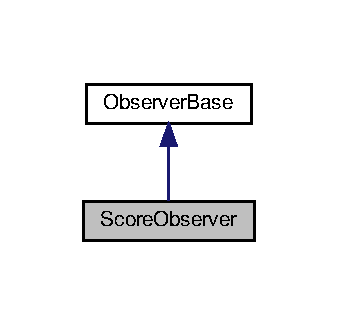
\includegraphics[width=162pt]{classScoreObserver__inherit__graph}
\end{center}
\end{figure}


Collaboration diagram for Score\+Observer\+:\nopagebreak
\begin{figure}[H]
\begin{center}
\leavevmode
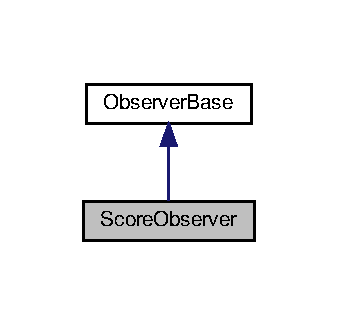
\includegraphics[width=162pt]{classScoreObserver__coll__graph}
\end{center}
\end{figure}
\subsection*{Public Member Functions}
\begin{DoxyCompactItemize}
\item 
\hyperlink{classScoreObserver_a29bf728993aedfded2ecf7c16df701cf}{Score\+Observer} ()
\item 
void \hyperlink{classScoreObserver_ad1b2727dbdc1f47de4b118a22fbdc12e}{update} (int amount) override
\item 
unsigned int \hyperlink{classScoreObserver_a99e163d5b7a3b53cdd9ae808a253235e}{get\+Score} () const
\end{DoxyCompactItemize}


\subsection{Constructor \& Destructor Documentation}
\mbox{\Hypertarget{classScoreObserver_a29bf728993aedfded2ecf7c16df701cf}\label{classScoreObserver_a29bf728993aedfded2ecf7c16df701cf}} 
\index{Score\+Observer@{Score\+Observer}!Score\+Observer@{Score\+Observer}}
\index{Score\+Observer@{Score\+Observer}!Score\+Observer@{Score\+Observer}}
\subsubsection{\texorpdfstring{Score\+Observer()}{ScoreObserver()}}
{\footnotesize\ttfamily Score\+Observer\+::\+Score\+Observer (\begin{DoxyParamCaption}{ }\end{DoxyParamCaption})}

default constructor 

\subsection{Member Function Documentation}
\mbox{\Hypertarget{classScoreObserver_a99e163d5b7a3b53cdd9ae808a253235e}\label{classScoreObserver_a99e163d5b7a3b53cdd9ae808a253235e}} 
\index{Score\+Observer@{Score\+Observer}!get\+Score@{get\+Score}}
\index{get\+Score@{get\+Score}!Score\+Observer@{Score\+Observer}}
\subsubsection{\texorpdfstring{get\+Score()}{getScore()}}
{\footnotesize\ttfamily unsigned int Score\+Observer\+::get\+Score (\begin{DoxyParamCaption}{ }\end{DoxyParamCaption}) const}

getter for m\+\_\+score \begin{DoxyReturn}{Returns}
the score stored in this observer 
\end{DoxyReturn}
\mbox{\Hypertarget{classScoreObserver_ad1b2727dbdc1f47de4b118a22fbdc12e}\label{classScoreObserver_ad1b2727dbdc1f47de4b118a22fbdc12e}} 
\index{Score\+Observer@{Score\+Observer}!update@{update}}
\index{update@{update}!Score\+Observer@{Score\+Observer}}
\subsubsection{\texorpdfstring{update()}{update()}}
{\footnotesize\ttfamily void Score\+Observer\+::update (\begin{DoxyParamCaption}\item[{int}]{amount }\end{DoxyParamCaption})\hspace{0.3cm}{\ttfamily [override]}, {\ttfamily [virtual]}}

update function overidded from observerbase 
\begin{DoxyParams}{Parameters}
{\em amount} & the amopunt of score that gets added \\
\hline
\end{DoxyParams}


Implements \hyperlink{classObserverBase}{Observer\+Base}.



The documentation for this class was generated from the following files\+:\begin{DoxyCompactItemize}
\item 
Game\+Logic/include/\+Observer/Score\+Observer.\+h\item 
Game\+Logic/\+Source/\+Observer/Score\+Observer.\+cpp\end{DoxyCompactItemize}

\hypertarget{classSFML__Entity__Factory}{}\section{S\+F\+M\+L\+\_\+\+Entity\+\_\+\+Factory Class Reference}
\label{classSFML__Entity__Factory}\index{S\+F\+M\+L\+\_\+\+Entity\+\_\+\+Factory@{S\+F\+M\+L\+\_\+\+Entity\+\_\+\+Factory}}


Inheritance diagram for S\+F\+M\+L\+\_\+\+Entity\+\_\+\+Factory\+:\nopagebreak
\begin{figure}[H]
\begin{center}
\leavevmode
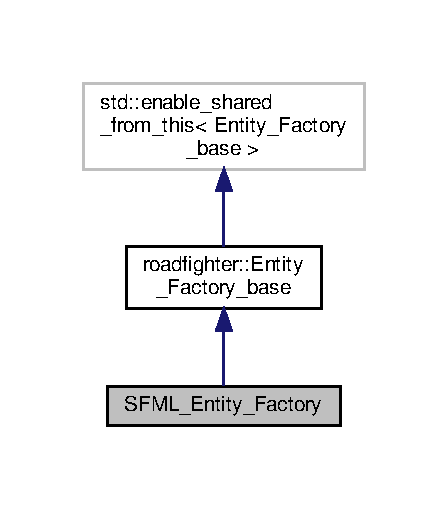
\includegraphics[width=215pt]{classSFML__Entity__Factory__inherit__graph}
\end{center}
\end{figure}


Collaboration diagram for S\+F\+M\+L\+\_\+\+Entity\+\_\+\+Factory\+:\nopagebreak
\begin{figure}[H]
\begin{center}
\leavevmode
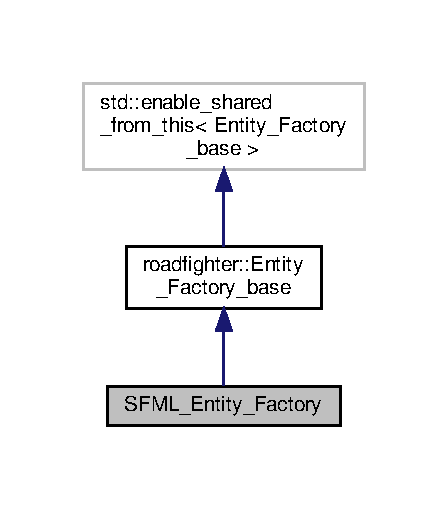
\includegraphics[width=215pt]{classSFML__Entity__Factory__coll__graph}
\end{center}
\end{figure}
\subsection*{Public Member Functions}
\begin{DoxyCompactItemize}
\item 
\mbox{\Hypertarget{classSFML__Entity__Factory_a615be01ab0a89f1cc1c8684ad38b94ae}\label{classSFML__Entity__Factory_a615be01ab0a89f1cc1c8684ad38b94ae}} 
{\bfseries S\+F\+M\+L\+\_\+\+Entity\+\_\+\+Factory} (const std\+::shared\+\_\+ptr$<$ sf\+::\+Render\+Window $>$ \&window)
\item 
std\+::shared\+\_\+ptr$<$ \hyperlink{classroadfighter_1_1Entity}{roadfighter\+::\+Entity} $>$ \hyperlink{classSFML__Entity__Factory_ab80783626b22a7746a8e9dd49e48e898}{create\+Bullet} (double x, double y, double v\+Speed) override
\item 
std\+::shared\+\_\+ptr$<$ \hyperlink{classroadfighter_1_1Entity}{roadfighter\+::\+Entity} $>$ \hyperlink{classSFML__Entity__Factory_afe1acae3b9c6d07ac30426a72ad390d0}{creat\+Passing\+Car} (double x, double y, double v\+Speedl) override
\item 
std\+::shared\+\_\+ptr$<$ \hyperlink{classroadfighter_1_1Entity}{roadfighter\+::\+Entity} $>$ \hyperlink{classSFML__Entity__Factory_a3c45cdbbfb31525bcdbee0ce87948236}{create\+Player\+Car} (double x, double y, double max, double v\+Accel, double h\+Accel, double fuel) override
\item 
std\+::shared\+\_\+ptr$<$ \hyperlink{classroadfighter_1_1Entity}{roadfighter\+::\+Entity} $>$ \hyperlink{classSFML__Entity__Factory_ac65176cfefa77f5f4af79f88ed244478}{create\+Racing\+Car} (double x, double y, double max, double v\+Accel, double h\+Accel) override
\item 
std\+::shared\+\_\+ptr$<$ \hyperlink{classroadfighter_1_1Entity}{roadfighter\+::\+Entity} $>$ \hyperlink{classSFML__Entity__Factory_a3a6743085eb4c1793be523fe07724328}{create\+World} () override
\item 
std\+::shared\+\_\+ptr$<$ \hyperlink{classroadfighter_1_1Entity}{roadfighter\+::\+Entity} $>$ \hyperlink{classSFML__Entity__Factory_af6fb01565b73487c90d93bc820603ca2}{create\+Bonus\+Car} (double x, double y, double v\+Speed) override
\item 
std\+::shared\+\_\+ptr$<$ \hyperlink{classroadfighter_1_1Entity}{roadfighter\+::\+Entity} $>$ \hyperlink{classSFML__Entity__Factory_af484c4ae7c9a82c171eb047fb05aa350}{create\+End} (double y) override
\end{DoxyCompactItemize}


\subsection{Member Function Documentation}
\mbox{\Hypertarget{classSFML__Entity__Factory_af6fb01565b73487c90d93bc820603ca2}\label{classSFML__Entity__Factory_af6fb01565b73487c90d93bc820603ca2}} 
\index{S\+F\+M\+L\+\_\+\+Entity\+\_\+\+Factory@{S\+F\+M\+L\+\_\+\+Entity\+\_\+\+Factory}!create\+Bonus\+Car@{create\+Bonus\+Car}}
\index{create\+Bonus\+Car@{create\+Bonus\+Car}!S\+F\+M\+L\+\_\+\+Entity\+\_\+\+Factory@{S\+F\+M\+L\+\_\+\+Entity\+\_\+\+Factory}}
\subsubsection{\texorpdfstring{create\+Bonus\+Car()}{createBonusCar()}}
{\footnotesize\ttfamily std\+::shared\+\_\+ptr$<$ \hyperlink{classroadfighter_1_1Entity}{roadfighter\+::\+Entity} $>$ S\+F\+M\+L\+\_\+\+Entity\+\_\+\+Factory\+::create\+Bonus\+Car (\begin{DoxyParamCaption}\item[{double}]{x,  }\item[{double}]{y,  }\item[{double}]{v\+Speed }\end{DoxyParamCaption})\hspace{0.3cm}{\ttfamily [override]}, {\ttfamily [virtual]}}

base factory method for creating a Bonus\+Car 
\begin{DoxyParams}{Parameters}
{\em x} & coordinate of the bonus car (the middle) \\
\hline
{\em y} & coordinate of the passing bonus car (the middle) \\
\hline
{\em v\+Speed} & the set speed of the passingcar \\
\hline
\end{DoxyParams}
\begin{DoxyReturn}{Returns}
a shared pointer to an entity 
\end{DoxyReturn}


Implements \hyperlink{classroadfighter_1_1Entity__Factory__base_a888f537d2deed2d90a391c1900e9fdb6}{roadfighter\+::\+Entity\+\_\+\+Factory\+\_\+base}.

\mbox{\Hypertarget{classSFML__Entity__Factory_ab80783626b22a7746a8e9dd49e48e898}\label{classSFML__Entity__Factory_ab80783626b22a7746a8e9dd49e48e898}} 
\index{S\+F\+M\+L\+\_\+\+Entity\+\_\+\+Factory@{S\+F\+M\+L\+\_\+\+Entity\+\_\+\+Factory}!create\+Bullet@{create\+Bullet}}
\index{create\+Bullet@{create\+Bullet}!S\+F\+M\+L\+\_\+\+Entity\+\_\+\+Factory@{S\+F\+M\+L\+\_\+\+Entity\+\_\+\+Factory}}
\subsubsection{\texorpdfstring{create\+Bullet()}{createBullet()}}
{\footnotesize\ttfamily std\+::shared\+\_\+ptr$<$ \hyperlink{classroadfighter_1_1Entity}{roadfighter\+::\+Entity} $>$ S\+F\+M\+L\+\_\+\+Entity\+\_\+\+Factory\+::create\+Bullet (\begin{DoxyParamCaption}\item[{double}]{x,  }\item[{double}]{y,  }\item[{double}]{v\+Speed }\end{DoxyParamCaption})\hspace{0.3cm}{\ttfamily [override]}, {\ttfamily [virtual]}}

base factory method for creating a bullet \begin{DoxyReturn}{Returns}
a shared pointer to an Entity 
\end{DoxyReturn}


Implements \hyperlink{classroadfighter_1_1Entity__Factory__base_a5241bdb886a9f1b086d009a0f6478045}{roadfighter\+::\+Entity\+\_\+\+Factory\+\_\+base}.

\mbox{\Hypertarget{classSFML__Entity__Factory_af484c4ae7c9a82c171eb047fb05aa350}\label{classSFML__Entity__Factory_af484c4ae7c9a82c171eb047fb05aa350}} 
\index{S\+F\+M\+L\+\_\+\+Entity\+\_\+\+Factory@{S\+F\+M\+L\+\_\+\+Entity\+\_\+\+Factory}!create\+End@{create\+End}}
\index{create\+End@{create\+End}!S\+F\+M\+L\+\_\+\+Entity\+\_\+\+Factory@{S\+F\+M\+L\+\_\+\+Entity\+\_\+\+Factory}}
\subsubsection{\texorpdfstring{create\+End()}{createEnd()}}
{\footnotesize\ttfamily std\+::shared\+\_\+ptr$<$ \hyperlink{classroadfighter_1_1Entity}{roadfighter\+::\+Entity} $>$ S\+F\+M\+L\+\_\+\+Entity\+\_\+\+Factory\+::create\+End (\begin{DoxyParamCaption}\item[{double}]{y }\end{DoxyParamCaption})\hspace{0.3cm}{\ttfamily [override]}, {\ttfamily [virtual]}}

base factory method for creating a End 
\begin{DoxyParams}{Parameters}
{\em y} & coordinate of the end \\
\hline
\end{DoxyParams}
\begin{DoxyReturn}{Returns}
a shared pointer to an entity 
\end{DoxyReturn}


Implements \hyperlink{classroadfighter_1_1Entity__Factory__base_a791574991ccbe7ff95f28e5651ed2cb1}{roadfighter\+::\+Entity\+\_\+\+Factory\+\_\+base}.

\mbox{\Hypertarget{classSFML__Entity__Factory_a3c45cdbbfb31525bcdbee0ce87948236}\label{classSFML__Entity__Factory_a3c45cdbbfb31525bcdbee0ce87948236}} 
\index{S\+F\+M\+L\+\_\+\+Entity\+\_\+\+Factory@{S\+F\+M\+L\+\_\+\+Entity\+\_\+\+Factory}!create\+Player\+Car@{create\+Player\+Car}}
\index{create\+Player\+Car@{create\+Player\+Car}!S\+F\+M\+L\+\_\+\+Entity\+\_\+\+Factory@{S\+F\+M\+L\+\_\+\+Entity\+\_\+\+Factory}}
\subsubsection{\texorpdfstring{create\+Player\+Car()}{createPlayerCar()}}
{\footnotesize\ttfamily std\+::shared\+\_\+ptr$<$ \hyperlink{classroadfighter_1_1Entity}{roadfighter\+::\+Entity} $>$ S\+F\+M\+L\+\_\+\+Entity\+\_\+\+Factory\+::create\+Player\+Car (\begin{DoxyParamCaption}\item[{double}]{x,  }\item[{double}]{y,  }\item[{double}]{max,  }\item[{double}]{v\+Accel,  }\item[{double}]{h\+Accel,  }\item[{double}]{fuel }\end{DoxyParamCaption})\hspace{0.3cm}{\ttfamily [override]}, {\ttfamily [virtual]}}

base factory method for crating the player car 
\begin{DoxyParams}{Parameters}
{\em x} & xoordinate of the player car (the middle) \\
\hline
{\em y} & coordinate of the player car (the middle) \\
\hline
{\em max} & the max vertical speed \\
\hline
{\em v\+Accel} & the vertical acceleration per tick \\
\hline
{\em h\+Accel} & the horizontal acceleration per tick \\
\hline
{\em fuel} & the starting fuel of the car \\
\hline
\end{DoxyParams}
\begin{DoxyReturn}{Returns}
a shared pointer to an entity 
\end{DoxyReturn}


Implements \hyperlink{classroadfighter_1_1Entity__Factory__base_a3021f69b62b9df33706096381664d58f}{roadfighter\+::\+Entity\+\_\+\+Factory\+\_\+base}.

\mbox{\Hypertarget{classSFML__Entity__Factory_ac65176cfefa77f5f4af79f88ed244478}\label{classSFML__Entity__Factory_ac65176cfefa77f5f4af79f88ed244478}} 
\index{S\+F\+M\+L\+\_\+\+Entity\+\_\+\+Factory@{S\+F\+M\+L\+\_\+\+Entity\+\_\+\+Factory}!create\+Racing\+Car@{create\+Racing\+Car}}
\index{create\+Racing\+Car@{create\+Racing\+Car}!S\+F\+M\+L\+\_\+\+Entity\+\_\+\+Factory@{S\+F\+M\+L\+\_\+\+Entity\+\_\+\+Factory}}
\subsubsection{\texorpdfstring{create\+Racing\+Car()}{createRacingCar()}}
{\footnotesize\ttfamily std\+::shared\+\_\+ptr$<$ \hyperlink{classroadfighter_1_1Entity}{roadfighter\+::\+Entity} $>$ S\+F\+M\+L\+\_\+\+Entity\+\_\+\+Factory\+::create\+Racing\+Car (\begin{DoxyParamCaption}\item[{double}]{x,  }\item[{double}]{y,  }\item[{double}]{max,  }\item[{double}]{v\+Accel,  }\item[{double}]{h\+Accel }\end{DoxyParamCaption})\hspace{0.3cm}{\ttfamily [override]}, {\ttfamily [virtual]}}

base factory method for crating a racing car 
\begin{DoxyParams}{Parameters}
{\em x} & xoordinate of the racing car (the middle) \\
\hline
{\em y} & coordinate of the racing car (the middle) \\
\hline
{\em max} & the max vertical speed \\
\hline
{\em v\+Accel} & the vertical acceleration per tick \\
\hline
{\em h\+Accel} & the horizontal acceleration per tick \\
\hline
\end{DoxyParams}
\begin{DoxyReturn}{Returns}
a shared pointer to an entity 
\end{DoxyReturn}


Implements \hyperlink{classroadfighter_1_1Entity__Factory__base_a17b9c30501b8a11624bee8f1c24a6b7e}{roadfighter\+::\+Entity\+\_\+\+Factory\+\_\+base}.

\mbox{\Hypertarget{classSFML__Entity__Factory_a3a6743085eb4c1793be523fe07724328}\label{classSFML__Entity__Factory_a3a6743085eb4c1793be523fe07724328}} 
\index{S\+F\+M\+L\+\_\+\+Entity\+\_\+\+Factory@{S\+F\+M\+L\+\_\+\+Entity\+\_\+\+Factory}!create\+World@{create\+World}}
\index{create\+World@{create\+World}!S\+F\+M\+L\+\_\+\+Entity\+\_\+\+Factory@{S\+F\+M\+L\+\_\+\+Entity\+\_\+\+Factory}}
\subsubsection{\texorpdfstring{create\+World()}{createWorld()}}
{\footnotesize\ttfamily std\+::shared\+\_\+ptr$<$ \hyperlink{classroadfighter_1_1Entity}{roadfighter\+::\+Entity} $>$ S\+F\+M\+L\+\_\+\+Entity\+\_\+\+Factory\+::create\+World (\begin{DoxyParamCaption}{ }\end{DoxyParamCaption})\hspace{0.3cm}{\ttfamily [override]}, {\ttfamily [virtual]}}

base factory method for creating the world \begin{DoxyReturn}{Returns}
a shared pointer to an enityt 
\end{DoxyReturn}


Implements \hyperlink{classroadfighter_1_1Entity__Factory__base_aa24de6bbeb80c25e96f3e24d6bcb5169}{roadfighter\+::\+Entity\+\_\+\+Factory\+\_\+base}.

\mbox{\Hypertarget{classSFML__Entity__Factory_afe1acae3b9c6d07ac30426a72ad390d0}\label{classSFML__Entity__Factory_afe1acae3b9c6d07ac30426a72ad390d0}} 
\index{S\+F\+M\+L\+\_\+\+Entity\+\_\+\+Factory@{S\+F\+M\+L\+\_\+\+Entity\+\_\+\+Factory}!creat\+Passing\+Car@{creat\+Passing\+Car}}
\index{creat\+Passing\+Car@{creat\+Passing\+Car}!S\+F\+M\+L\+\_\+\+Entity\+\_\+\+Factory@{S\+F\+M\+L\+\_\+\+Entity\+\_\+\+Factory}}
\subsubsection{\texorpdfstring{creat\+Passing\+Car()}{creatPassingCar()}}
{\footnotesize\ttfamily std\+::shared\+\_\+ptr$<$ \hyperlink{classroadfighter_1_1Entity}{roadfighter\+::\+Entity} $>$ S\+F\+M\+L\+\_\+\+Entity\+\_\+\+Factory\+::creat\+Passing\+Car (\begin{DoxyParamCaption}\item[{double}]{x,  }\item[{double}]{y,  }\item[{double}]{v\+Speed }\end{DoxyParamCaption})\hspace{0.3cm}{\ttfamily [override]}, {\ttfamily [virtual]}}

base factory method for creating a Passing\+Car 
\begin{DoxyParams}{Parameters}
{\em x} & coordinate of the passing car (the middle) \\
\hline
{\em y} & coordinate of the passing car (the middle) \\
\hline
{\em v\+Speed} & the set speed of the passingcar \\
\hline
\end{DoxyParams}
\begin{DoxyReturn}{Returns}
a shared pointer to an entity 
\end{DoxyReturn}


Implements \hyperlink{classroadfighter_1_1Entity__Factory__base_aa21b8cb23696844b7349ccf2c87d10fa}{roadfighter\+::\+Entity\+\_\+\+Factory\+\_\+base}.



The documentation for this class was generated from the following files\+:\begin{DoxyCompactItemize}
\item 
S\+F\+M\+L\+Conversion/\+Include/S\+F\+M\+L\+\_\+\+Entity\+\_\+\+Factory.\+h\item 
S\+F\+M\+L\+Conversion/\+Source/S\+F\+M\+L\+\_\+\+Entity\+\_\+\+Factory.\+cpp\end{DoxyCompactItemize}

\hypertarget{classSFMLBonusCar}{}\section{S\+F\+M\+L\+Bonus\+Car Class Reference}
\label{classSFMLBonusCar}\index{S\+F\+M\+L\+Bonus\+Car@{S\+F\+M\+L\+Bonus\+Car}}


Inheritance diagram for S\+F\+M\+L\+Bonus\+Car\+:\nopagebreak
\begin{figure}[H]
\begin{center}
\leavevmode
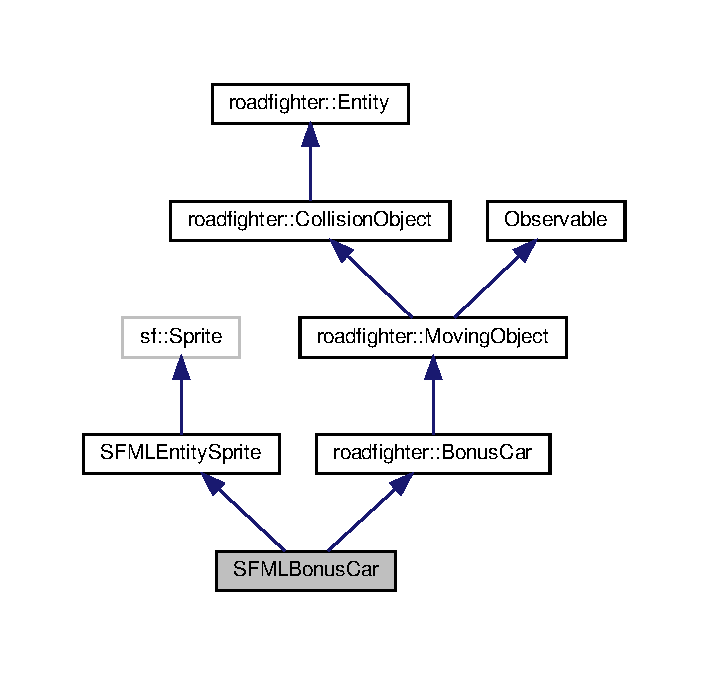
\includegraphics[width=340pt]{classSFMLBonusCar__inherit__graph}
\end{center}
\end{figure}


Collaboration diagram for S\+F\+M\+L\+Bonus\+Car\+:\nopagebreak
\begin{figure}[H]
\begin{center}
\leavevmode
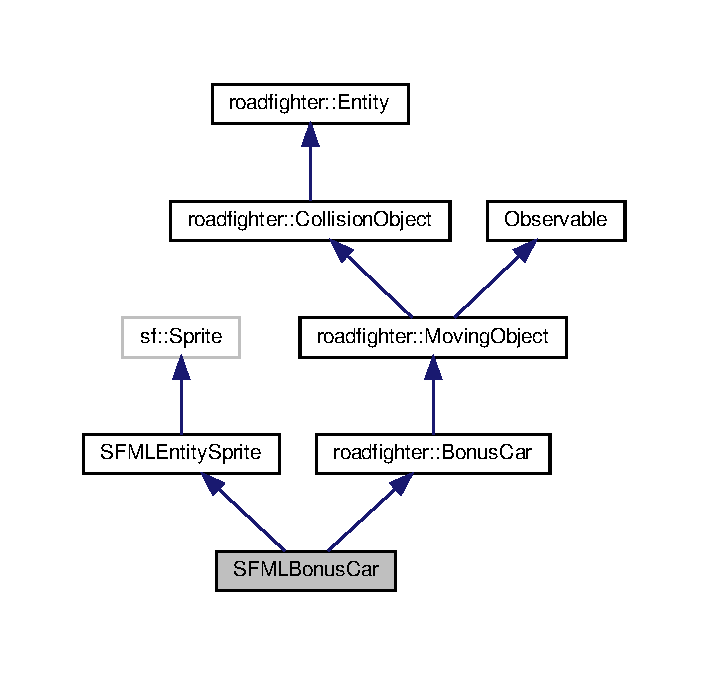
\includegraphics[width=340pt]{classSFMLBonusCar__coll__graph}
\end{center}
\end{figure}
\subsection*{Public Member Functions}
\begin{DoxyCompactItemize}
\item 
\mbox{\Hypertarget{classSFMLBonusCar_a891d1bc1e689c6343799ea8984ef2f9e}\label{classSFMLBonusCar_a891d1bc1e689c6343799ea8984ef2f9e}} 
{\bfseries S\+F\+M\+L\+Bonus\+Car} (const std\+::shared\+\_\+ptr$<$ sf\+::\+Render\+Window $>$ \&window, const \hyperlink{classroadfighter_1_1Location}{roadfighter\+::\+Location} \&m\+\_\+loc1, const \hyperlink{classroadfighter_1_1Location}{roadfighter\+::\+Location} \&m\+\_\+loc2, double vert\+Speed)
\item 
void \hyperlink{classSFMLBonusCar_a95d6a17fdbd099db1fe080da1581da20}{draw} () override
\end{DoxyCompactItemize}


\subsection{Member Function Documentation}
\mbox{\Hypertarget{classSFMLBonusCar_a95d6a17fdbd099db1fe080da1581da20}\label{classSFMLBonusCar_a95d6a17fdbd099db1fe080da1581da20}} 
\index{S\+F\+M\+L\+Bonus\+Car@{S\+F\+M\+L\+Bonus\+Car}!draw@{draw}}
\index{draw@{draw}!S\+F\+M\+L\+Bonus\+Car@{S\+F\+M\+L\+Bonus\+Car}}
\subsubsection{\texorpdfstring{draw()}{draw()}}
{\footnotesize\ttfamily void S\+F\+M\+L\+Bonus\+Car\+::draw (\begin{DoxyParamCaption}{ }\end{DoxyParamCaption})\hspace{0.3cm}{\ttfamily [override]}, {\ttfamily [virtual]}}

virtual void function that is used to draw the entity this function is not overriden in the game logic itself and should be implemented by the creator of the graphics implementation 

Implements \hyperlink{classroadfighter_1_1Entity_ac516f8005f969ad5a86c252e5a3640ee}{roadfighter\+::\+Entity}.



The documentation for this class was generated from the following files\+:\begin{DoxyCompactItemize}
\item 
S\+F\+M\+L\+Conversion/\+Include/\+Entities/S\+F\+M\+L\+Bonus\+Car.\+h\item 
S\+F\+M\+L\+Conversion/\+Source/entities/S\+F\+M\+L\+Bonus\+Car.\+cpp\end{DoxyCompactItemize}

\hypertarget{classSFMLBullet}{}\section{S\+F\+M\+L\+Bullet Class Reference}
\label{classSFMLBullet}\index{S\+F\+M\+L\+Bullet@{S\+F\+M\+L\+Bullet}}


Inheritance diagram for S\+F\+M\+L\+Bullet\+:\nopagebreak
\begin{figure}[H]
\begin{center}
\leavevmode
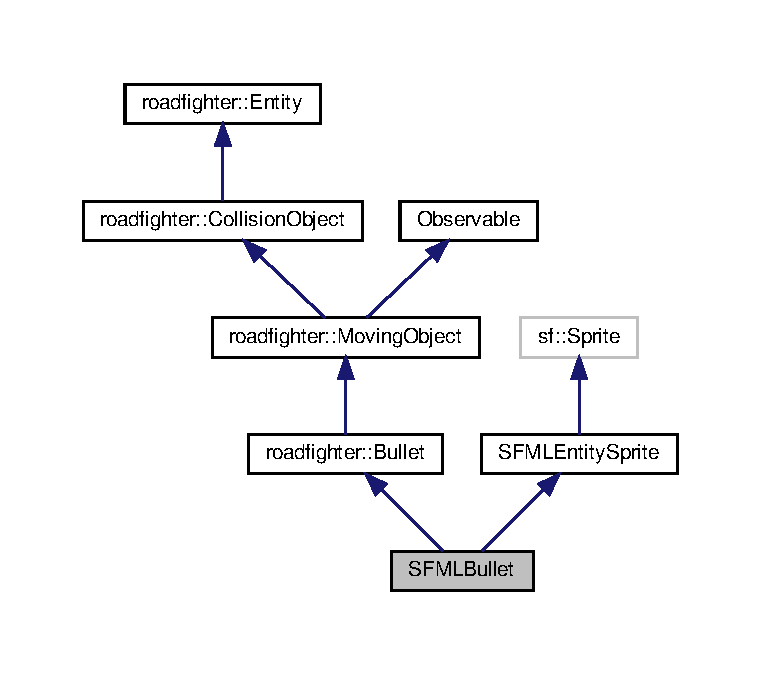
\includegraphics[width=350pt]{classSFMLBullet__inherit__graph}
\end{center}
\end{figure}


Collaboration diagram for S\+F\+M\+L\+Bullet\+:\nopagebreak
\begin{figure}[H]
\begin{center}
\leavevmode
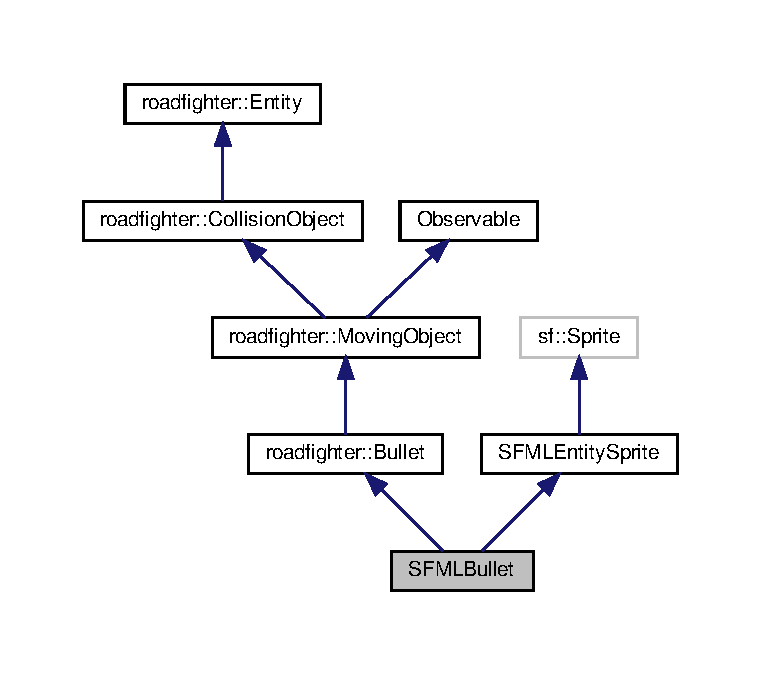
\includegraphics[width=350pt]{classSFMLBullet__coll__graph}
\end{center}
\end{figure}
\subsection*{Public Member Functions}
\begin{DoxyCompactItemize}
\item 
\mbox{\Hypertarget{classSFMLBullet_a2b3500037bdd26f039c24fc0f8d9ddeb}\label{classSFMLBullet_a2b3500037bdd26f039c24fc0f8d9ddeb}} 
{\bfseries S\+F\+M\+L\+Bullet} (const \hyperlink{classroadfighter_1_1Location}{roadfighter\+::\+Location} \&m\+\_\+loc1, const \hyperlink{classroadfighter_1_1Location}{roadfighter\+::\+Location} \&m\+\_\+loc2, double vertspeed, const std\+::shared\+\_\+ptr$<$ sf\+::\+Render\+Window $>$ \&window)
\item 
void \hyperlink{classSFMLBullet_a2b774898d1f369ab6d1e58659dab389a}{draw} () override
\end{DoxyCompactItemize}


\subsection{Member Function Documentation}
\mbox{\Hypertarget{classSFMLBullet_a2b774898d1f369ab6d1e58659dab389a}\label{classSFMLBullet_a2b774898d1f369ab6d1e58659dab389a}} 
\index{S\+F\+M\+L\+Bullet@{S\+F\+M\+L\+Bullet}!draw@{draw}}
\index{draw@{draw}!S\+F\+M\+L\+Bullet@{S\+F\+M\+L\+Bullet}}
\subsubsection{\texorpdfstring{draw()}{draw()}}
{\footnotesize\ttfamily void S\+F\+M\+L\+Bullet\+::draw (\begin{DoxyParamCaption}{ }\end{DoxyParamCaption})\hspace{0.3cm}{\ttfamily [override]}, {\ttfamily [virtual]}}

virtual void function that is used to draw the entity this function is not overriden in the game logic itself and should be implemented by the creator of the graphics implementation 

Implements \hyperlink{classroadfighter_1_1Entity_ac516f8005f969ad5a86c252e5a3640ee}{roadfighter\+::\+Entity}.



The documentation for this class was generated from the following files\+:\begin{DoxyCompactItemize}
\item 
S\+F\+M\+L\+Conversion/\+Include/\+Entities/S\+F\+M\+L\+Bullet.\+h\item 
S\+F\+M\+L\+Conversion/\+Source/entities/S\+F\+M\+L\+Bullet.\+cpp\end{DoxyCompactItemize}

\hypertarget{classSFMLEnd}{}\section{S\+F\+M\+L\+End Class Reference}
\label{classSFMLEnd}\index{S\+F\+M\+L\+End@{S\+F\+M\+L\+End}}


Inheritance diagram for S\+F\+M\+L\+End\+:\nopagebreak
\begin{figure}[H]
\begin{center}
\leavevmode
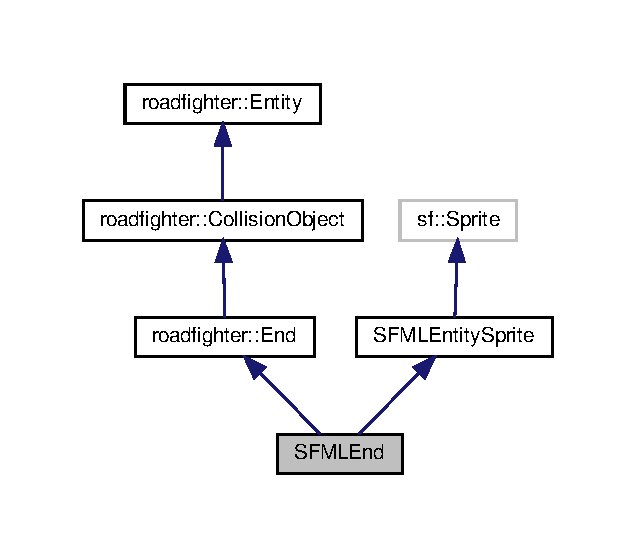
\includegraphics[width=305pt]{classSFMLEnd__inherit__graph}
\end{center}
\end{figure}


Collaboration diagram for S\+F\+M\+L\+End\+:\nopagebreak
\begin{figure}[H]
\begin{center}
\leavevmode
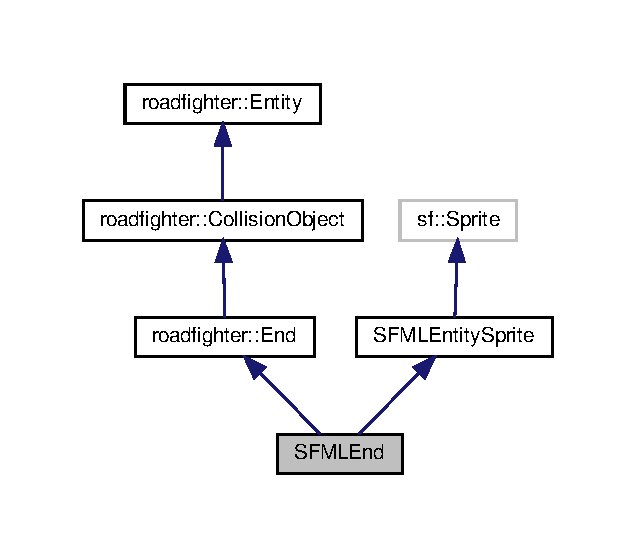
\includegraphics[width=305pt]{classSFMLEnd__coll__graph}
\end{center}
\end{figure}
\subsection*{Public Member Functions}
\begin{DoxyCompactItemize}
\item 
\mbox{\Hypertarget{classSFMLEnd_acf2db930f449f1995d98216fffdea1ec}\label{classSFMLEnd_acf2db930f449f1995d98216fffdea1ec}} 
{\bfseries S\+F\+M\+L\+End} (const \hyperlink{classroadfighter_1_1Location}{roadfighter\+::\+Location} \&m\+\_\+loc1, const \hyperlink{classroadfighter_1_1Location}{roadfighter\+::\+Location} \&m\+\_\+loc2, const std\+::shared\+\_\+ptr$<$ sf\+::\+Render\+Window $>$ \&window)
\item 
void \hyperlink{classSFMLEnd_aee51982a63f9c1c6495f539528683989}{draw} () override
\end{DoxyCompactItemize}


\subsection{Member Function Documentation}
\mbox{\Hypertarget{classSFMLEnd_aee51982a63f9c1c6495f539528683989}\label{classSFMLEnd_aee51982a63f9c1c6495f539528683989}} 
\index{S\+F\+M\+L\+End@{S\+F\+M\+L\+End}!draw@{draw}}
\index{draw@{draw}!S\+F\+M\+L\+End@{S\+F\+M\+L\+End}}
\subsubsection{\texorpdfstring{draw()}{draw()}}
{\footnotesize\ttfamily void S\+F\+M\+L\+End\+::draw (\begin{DoxyParamCaption}{ }\end{DoxyParamCaption})\hspace{0.3cm}{\ttfamily [override]}, {\ttfamily [virtual]}}

virtual void function that is used to draw the entity this function is not overriden in the game logic itself and should be implemented by the creator of the graphics implementation 

Implements \hyperlink{classroadfighter_1_1Entity_ac516f8005f969ad5a86c252e5a3640ee}{roadfighter\+::\+Entity}.



The documentation for this class was generated from the following files\+:\begin{DoxyCompactItemize}
\item 
S\+F\+M\+L\+Conversion/\+Include/\+Entities/S\+F\+M\+L\+End.\+h\item 
S\+F\+M\+L\+Conversion/\+Source/entities/S\+F\+M\+L\+End.\+cpp\end{DoxyCompactItemize}

\hypertarget{classSFMLEntitySprite}{}\section{S\+F\+M\+L\+Entity\+Sprite Class Reference}
\label{classSFMLEntitySprite}\index{S\+F\+M\+L\+Entity\+Sprite@{S\+F\+M\+L\+Entity\+Sprite}}


Inheritance diagram for S\+F\+M\+L\+Entity\+Sprite\+:\nopagebreak
\begin{figure}[H]
\begin{center}
\leavevmode
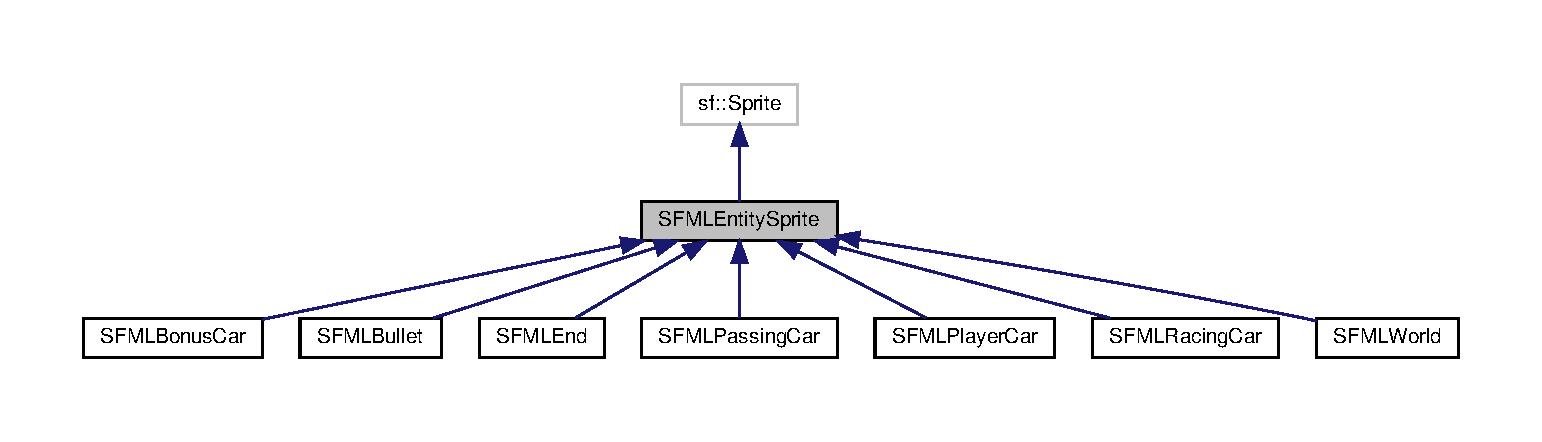
\includegraphics[width=350pt]{classSFMLEntitySprite__inherit__graph}
\end{center}
\end{figure}


Collaboration diagram for S\+F\+M\+L\+Entity\+Sprite\+:\nopagebreak
\begin{figure}[H]
\begin{center}
\leavevmode
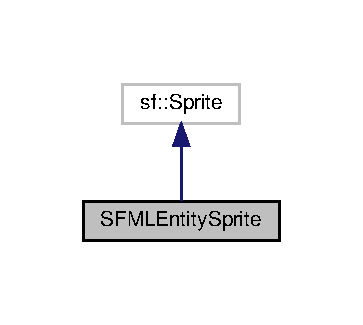
\includegraphics[width=174pt]{classSFMLEntitySprite__coll__graph}
\end{center}
\end{figure}
\subsection*{Public Member Functions}
\begin{DoxyCompactItemize}
\item 
\mbox{\Hypertarget{classSFMLEntitySprite_a70480096b35a12e360ebb76fc10e958f}\label{classSFMLEntitySprite_a70480096b35a12e360ebb76fc10e958f}} 
{\bfseries S\+F\+M\+L\+Entity\+Sprite} (const std\+::string \&path, std\+::shared\+\_\+ptr$<$ sf\+::\+Render\+Window $>$ window)
\item 
\mbox{\Hypertarget{classSFMLEntitySprite_af27155ca269dc50239c6ef57d03dedaf}\label{classSFMLEntitySprite_af27155ca269dc50239c6ef57d03dedaf}} 
void {\bfseries set\+Sprite\+Location} (double x, double y)
\item 
\mbox{\Hypertarget{classSFMLEntitySprite_af831d4a79aec4370c15f22f2dc86433e}\label{classSFMLEntitySprite_af831d4a79aec4370c15f22f2dc86433e}} 
void {\bfseries set\+Sprite\+Size} (double width, double height)
\item 
\mbox{\Hypertarget{classSFMLEntitySprite_a65526a721915827363cbfc32c9cf8b61}\label{classSFMLEntitySprite_a65526a721915827363cbfc32c9cf8b61}} 
void {\bfseries load\+Sprite} (const std\+::string \&path)
\item 
\mbox{\Hypertarget{classSFMLEntitySprite_ac285372cd7a7d8413ccb52c2d0699376}\label{classSFMLEntitySprite_ac285372cd7a7d8413ccb52c2d0699376}} 
const std\+::shared\+\_\+ptr$<$ sf\+::\+Render\+Window $>$ \& {\bfseries get\+Window} () const
\end{DoxyCompactItemize}


The documentation for this class was generated from the following files\+:\begin{DoxyCompactItemize}
\item 
S\+F\+M\+L\+Conversion/\+Include/\+Entities/S\+F\+M\+L\+Entity\+Sprite.\+h\item 
S\+F\+M\+L\+Conversion/\+Source/entities/S\+F\+M\+L\+Entity\+Sprite.\+cpp\end{DoxyCompactItemize}

\hypertarget{classSFMLPassingCar}{}\section{S\+F\+M\+L\+Passing\+Car Class Reference}
\label{classSFMLPassingCar}\index{S\+F\+M\+L\+Passing\+Car@{S\+F\+M\+L\+Passing\+Car}}


Inheritance diagram for S\+F\+M\+L\+Passing\+Car\+:\nopagebreak
\begin{figure}[H]
\begin{center}
\leavevmode
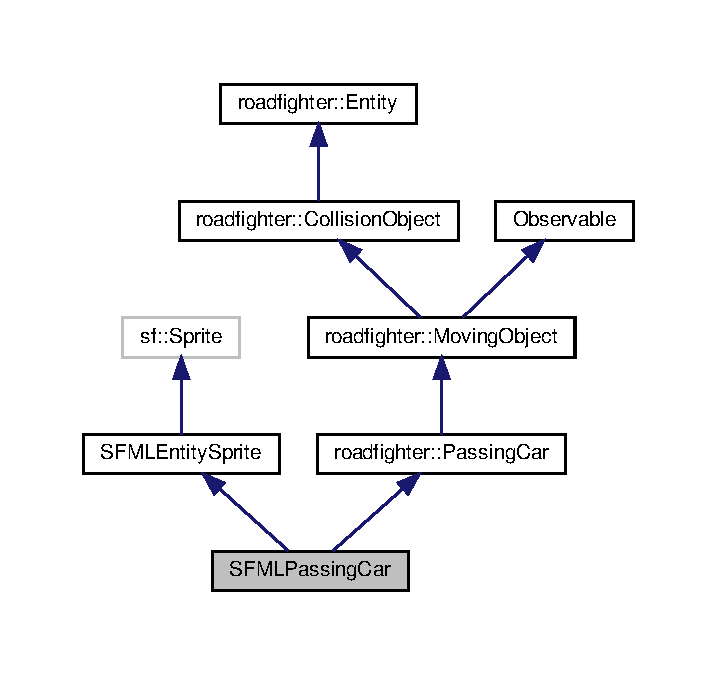
\includegraphics[width=344pt]{classSFMLPassingCar__inherit__graph}
\end{center}
\end{figure}


Collaboration diagram for S\+F\+M\+L\+Passing\+Car\+:\nopagebreak
\begin{figure}[H]
\begin{center}
\leavevmode
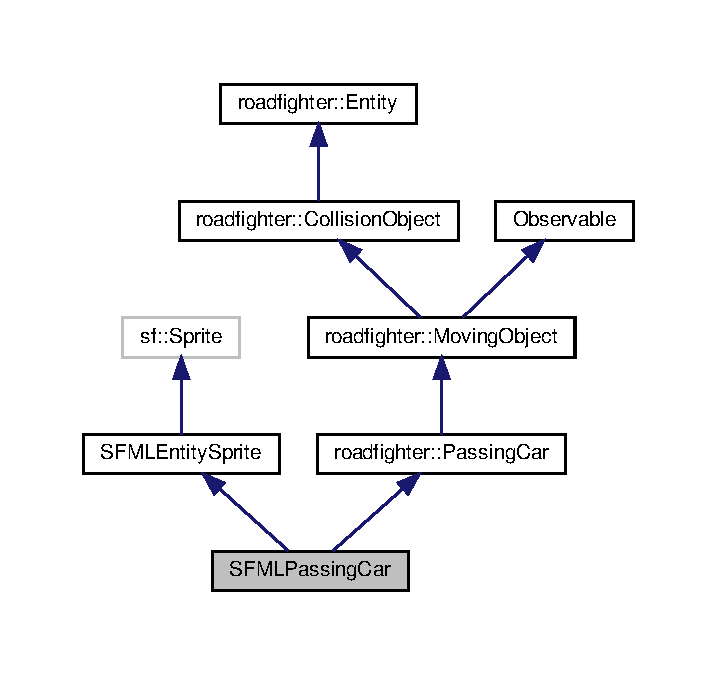
\includegraphics[width=344pt]{classSFMLPassingCar__coll__graph}
\end{center}
\end{figure}
\subsection*{Public Member Functions}
\begin{DoxyCompactItemize}
\item 
\mbox{\Hypertarget{classSFMLPassingCar_a8011df3b42eb3b0fa11c7a55f9ac5400}\label{classSFMLPassingCar_a8011df3b42eb3b0fa11c7a55f9ac5400}} 
{\bfseries S\+F\+M\+L\+Passing\+Car} (const std\+::shared\+\_\+ptr$<$ sf\+::\+Render\+Window $>$ \&window, const \hyperlink{classroadfighter_1_1Location}{roadfighter\+::\+Location} \&m\+\_\+loc1, const \hyperlink{classroadfighter_1_1Location}{roadfighter\+::\+Location} \&m\+\_\+loc2, double vert\+Speed)
\item 
void \hyperlink{classSFMLPassingCar_ad860ff5f0eea98fffaa51381c9424e8d}{draw} () override
\end{DoxyCompactItemize}


\subsection{Member Function Documentation}
\mbox{\Hypertarget{classSFMLPassingCar_ad860ff5f0eea98fffaa51381c9424e8d}\label{classSFMLPassingCar_ad860ff5f0eea98fffaa51381c9424e8d}} 
\index{S\+F\+M\+L\+Passing\+Car@{S\+F\+M\+L\+Passing\+Car}!draw@{draw}}
\index{draw@{draw}!S\+F\+M\+L\+Passing\+Car@{S\+F\+M\+L\+Passing\+Car}}
\subsubsection{\texorpdfstring{draw()}{draw()}}
{\footnotesize\ttfamily void S\+F\+M\+L\+Passing\+Car\+::draw (\begin{DoxyParamCaption}{ }\end{DoxyParamCaption})\hspace{0.3cm}{\ttfamily [override]}, {\ttfamily [virtual]}}

virtual void function that is used to draw the entity this function is not overriden in the game logic itself and should be implemented by the creator of the graphics implementation 

Implements \hyperlink{classroadfighter_1_1Entity_ac516f8005f969ad5a86c252e5a3640ee}{roadfighter\+::\+Entity}.



The documentation for this class was generated from the following files\+:\begin{DoxyCompactItemize}
\item 
S\+F\+M\+L\+Conversion/\+Include/\+Entities/S\+F\+M\+L\+Passing\+Car.\+h\item 
S\+F\+M\+L\+Conversion/\+Source/entities/S\+F\+M\+L\+Passing\+Car.\+cpp\end{DoxyCompactItemize}

\hypertarget{classSFMLPlayerCar}{}\section{S\+F\+M\+L\+Player\+Car Class Reference}
\label{classSFMLPlayerCar}\index{S\+F\+M\+L\+Player\+Car@{S\+F\+M\+L\+Player\+Car}}


Inheritance diagram for S\+F\+M\+L\+Player\+Car\+:\nopagebreak
\begin{figure}[H]
\begin{center}
\leavevmode
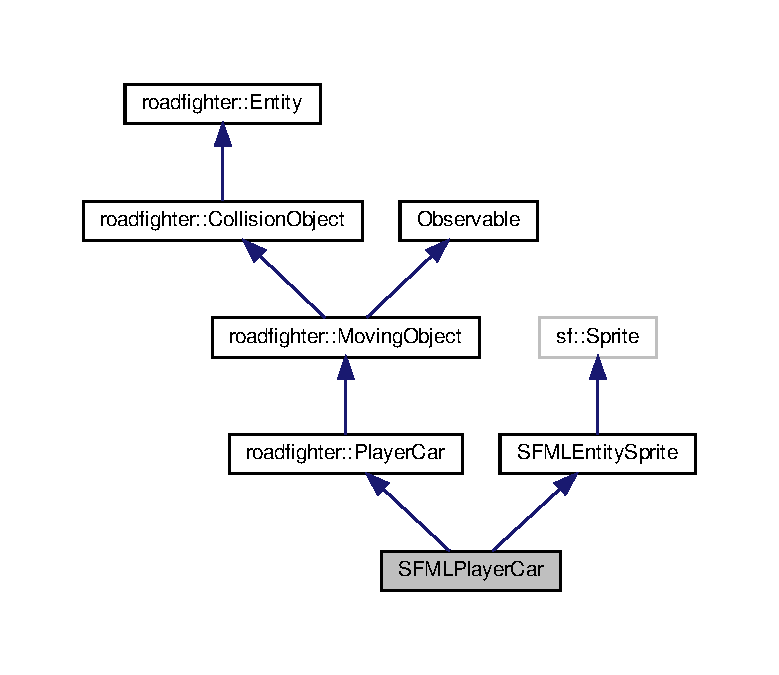
\includegraphics[width=350pt]{classSFMLPlayerCar__inherit__graph}
\end{center}
\end{figure}


Collaboration diagram for S\+F\+M\+L\+Player\+Car\+:\nopagebreak
\begin{figure}[H]
\begin{center}
\leavevmode
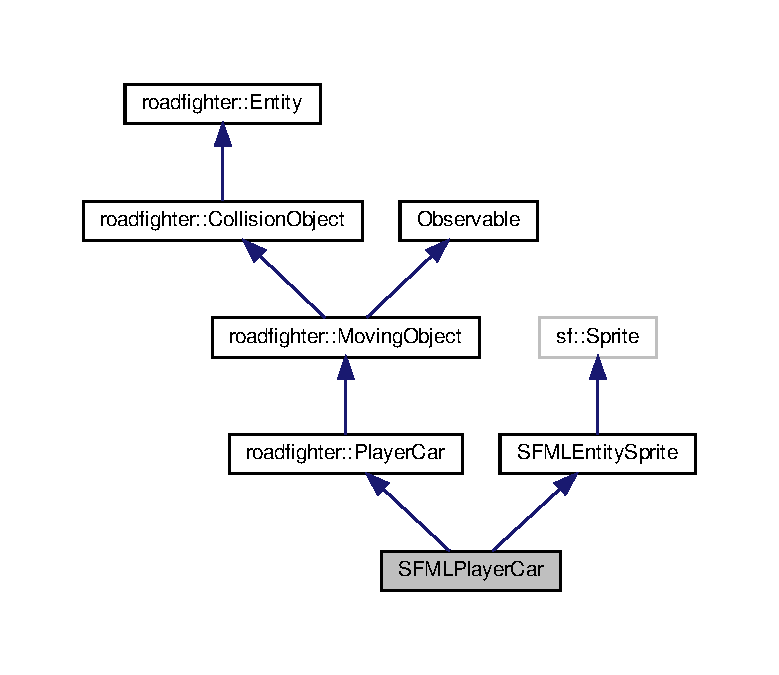
\includegraphics[width=350pt]{classSFMLPlayerCar__coll__graph}
\end{center}
\end{figure}
\subsection*{Public Member Functions}
\begin{DoxyCompactItemize}
\item 
\mbox{\Hypertarget{classSFMLPlayerCar_a9abc7243272952e87a6fe14973184e37}\label{classSFMLPlayerCar_a9abc7243272952e87a6fe14973184e37}} 
{\bfseries S\+F\+M\+L\+Player\+Car} (const \hyperlink{classroadfighter_1_1Location}{roadfighter\+::\+Location} \&m\+\_\+loc1, const \hyperlink{classroadfighter_1_1Location}{roadfighter\+::\+Location} \&m\+\_\+loc2, double m\+\_\+max\+Vert\+Speed, double m\+\_\+vert\+Accel, double m\+\_\+hor\+Accel, double m\+\_\+fuel, const std\+::shared\+\_\+ptr$<$ \hyperlink{classroadfighter_1_1InputController}{roadfighter\+::\+Input\+Controller} $>$ \&m\+\_\+move\+Controller, const std\+::shared\+\_\+ptr$<$ \hyperlink{classroadfighter_1_1EntityTransporter}{roadfighter\+::\+Entity\+Transporter} $>$ \&transporter, const std\+::shared\+\_\+ptr$<$ \hyperlink{classroadfighter_1_1Entity__Factory__base}{roadfighter\+::\+Entity\+\_\+\+Factory\+\_\+base} $>$ \&factory, const std\+::shared\+\_\+ptr$<$ sf\+::\+Render\+Window $>$ \&window)
\item 
void \hyperlink{classSFMLPlayerCar_ab4adedb2554e5f5eb59b7565a592c2b2}{draw} () override
\end{DoxyCompactItemize}


\subsection{Member Function Documentation}
\mbox{\Hypertarget{classSFMLPlayerCar_ab4adedb2554e5f5eb59b7565a592c2b2}\label{classSFMLPlayerCar_ab4adedb2554e5f5eb59b7565a592c2b2}} 
\index{S\+F\+M\+L\+Player\+Car@{S\+F\+M\+L\+Player\+Car}!draw@{draw}}
\index{draw@{draw}!S\+F\+M\+L\+Player\+Car@{S\+F\+M\+L\+Player\+Car}}
\subsubsection{\texorpdfstring{draw()}{draw()}}
{\footnotesize\ttfamily void S\+F\+M\+L\+Player\+Car\+::draw (\begin{DoxyParamCaption}{ }\end{DoxyParamCaption})\hspace{0.3cm}{\ttfamily [override]}, {\ttfamily [virtual]}}

virtual void function that is used to draw the entity this function is not overriden in the game logic itself and should be implemented by the creator of the graphics implementation 

Implements \hyperlink{classroadfighter_1_1Entity_ac516f8005f969ad5a86c252e5a3640ee}{roadfighter\+::\+Entity}.



The documentation for this class was generated from the following files\+:\begin{DoxyCompactItemize}
\item 
S\+F\+M\+L\+Conversion/\+Include/\+Entities/S\+F\+M\+L\+Player\+Car.\+h\item 
S\+F\+M\+L\+Conversion/\+Source/entities/S\+F\+M\+L\+Player\+Car.\+cpp\end{DoxyCompactItemize}

\hypertarget{classSFMLRacingCar}{}\section{S\+F\+M\+L\+Racing\+Car Class Reference}
\label{classSFMLRacingCar}\index{S\+F\+M\+L\+Racing\+Car@{S\+F\+M\+L\+Racing\+Car}}


Inheritance diagram for S\+F\+M\+L\+Racing\+Car\+:\nopagebreak
\begin{figure}[H]
\begin{center}
\leavevmode
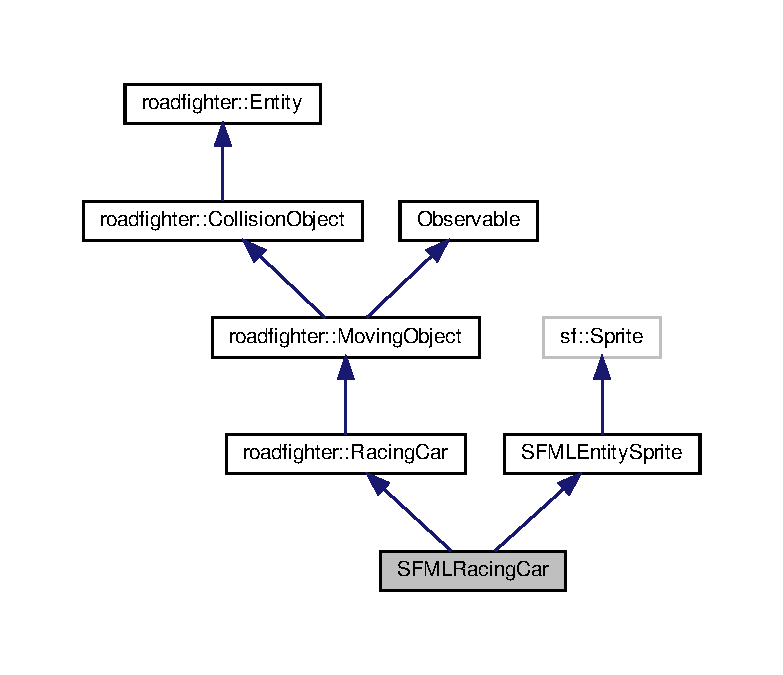
\includegraphics[width=350pt]{classSFMLRacingCar__inherit__graph}
\end{center}
\end{figure}


Collaboration diagram for S\+F\+M\+L\+Racing\+Car\+:\nopagebreak
\begin{figure}[H]
\begin{center}
\leavevmode
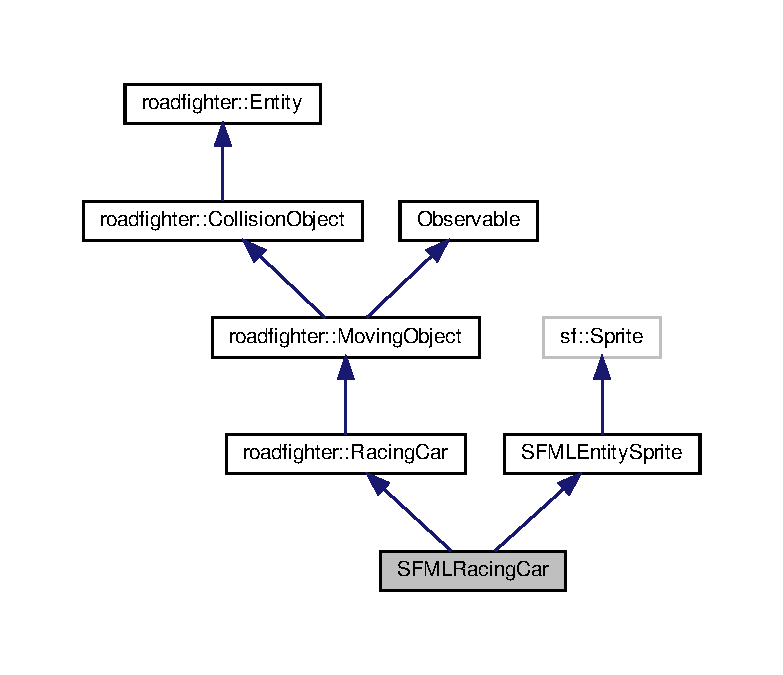
\includegraphics[width=350pt]{classSFMLRacingCar__coll__graph}
\end{center}
\end{figure}
\subsection*{Public Member Functions}
\begin{DoxyCompactItemize}
\item 
\mbox{\Hypertarget{classSFMLRacingCar_a88403a7946e3b8c4174bff103110f8c1}\label{classSFMLRacingCar_a88403a7946e3b8c4174bff103110f8c1}} 
{\bfseries S\+F\+M\+L\+Racing\+Car} (const \hyperlink{classroadfighter_1_1Location}{roadfighter\+::\+Location} \&m\+\_\+loc1, const \hyperlink{classroadfighter_1_1Location}{roadfighter\+::\+Location} \&m\+\_\+loc2, double m\+\_\+max\+Vert\+Speed, double m\+\_\+vert\+Accel, double m\+\_\+hor\+Accel, const std\+::shared\+\_\+ptr$<$ sf\+::\+Render\+Window $>$ \&window)
\item 
void \hyperlink{classSFMLRacingCar_a2b1c8b9ad2b80c9e18990cb078d2d62d}{draw} () override
\end{DoxyCompactItemize}


\subsection{Member Function Documentation}
\mbox{\Hypertarget{classSFMLRacingCar_a2b1c8b9ad2b80c9e18990cb078d2d62d}\label{classSFMLRacingCar_a2b1c8b9ad2b80c9e18990cb078d2d62d}} 
\index{S\+F\+M\+L\+Racing\+Car@{S\+F\+M\+L\+Racing\+Car}!draw@{draw}}
\index{draw@{draw}!S\+F\+M\+L\+Racing\+Car@{S\+F\+M\+L\+Racing\+Car}}
\subsubsection{\texorpdfstring{draw()}{draw()}}
{\footnotesize\ttfamily void S\+F\+M\+L\+Racing\+Car\+::draw (\begin{DoxyParamCaption}{ }\end{DoxyParamCaption})\hspace{0.3cm}{\ttfamily [override]}, {\ttfamily [virtual]}}

virtual void function that is used to draw the entity this function is not overriden in the game logic itself and should be implemented by the creator of the graphics implementation 

Implements \hyperlink{classroadfighter_1_1Entity_ac516f8005f969ad5a86c252e5a3640ee}{roadfighter\+::\+Entity}.



The documentation for this class was generated from the following files\+:\begin{DoxyCompactItemize}
\item 
S\+F\+M\+L\+Conversion/\+Include/\+Entities/S\+F\+M\+L\+Racing\+Car.\+h\item 
S\+F\+M\+L\+Conversion/\+Source/entities/S\+F\+M\+L\+Racing\+Car.\+cpp\end{DoxyCompactItemize}

\hypertarget{classSFMLRoadFighter}{}\section{S\+F\+M\+L\+Road\+Fighter Class Reference}
\label{classSFMLRoadFighter}\index{S\+F\+M\+L\+Road\+Fighter@{S\+F\+M\+L\+Road\+Fighter}}
\subsection*{Public Member Functions}
\begin{DoxyCompactItemize}
\item 
\mbox{\Hypertarget{classSFMLRoadFighter_a0f3bf2fc0d057aac66fbc68d87fba175}\label{classSFMLRoadFighter_a0f3bf2fc0d057aac66fbc68d87fba175}} 
void {\bfseries rungame} ()
\end{DoxyCompactItemize}


The documentation for this class was generated from the following files\+:\begin{DoxyCompactItemize}
\item 
S\+F\+M\+L\+Conversion/\+Include/S\+F\+M\+L\+Road\+Fighter.\+h\item 
S\+F\+M\+L\+Conversion/\+Source/S\+F\+M\+L\+Road\+Fighter.\+cpp\end{DoxyCompactItemize}

\hypertarget{classSFMLWorld}{}\section{S\+F\+M\+L\+World Class Reference}
\label{classSFMLWorld}\index{S\+F\+M\+L\+World@{S\+F\+M\+L\+World}}


Inheritance diagram for S\+F\+M\+L\+World\+:\nopagebreak
\begin{figure}[H]
\begin{center}
\leavevmode
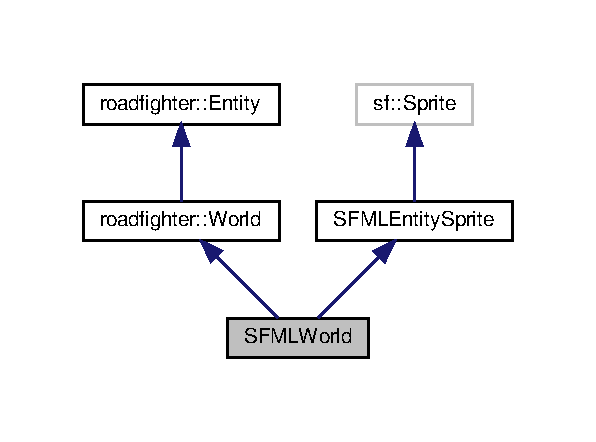
\includegraphics[width=286pt]{classSFMLWorld__inherit__graph}
\end{center}
\end{figure}


Collaboration diagram for S\+F\+M\+L\+World\+:\nopagebreak
\begin{figure}[H]
\begin{center}
\leavevmode
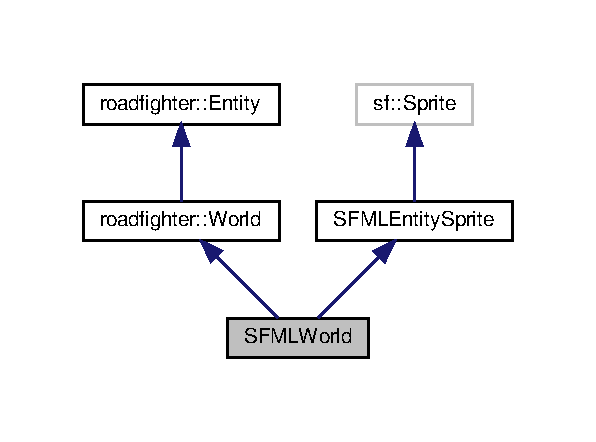
\includegraphics[width=286pt]{classSFMLWorld__coll__graph}
\end{center}
\end{figure}
\subsection*{Public Member Functions}
\begin{DoxyCompactItemize}
\item 
\mbox{\Hypertarget{classSFMLWorld_a44e744c66e65d0cff6a76b68f281f566}\label{classSFMLWorld_a44e744c66e65d0cff6a76b68f281f566}} 
{\bfseries S\+F\+M\+L\+World} (const std\+::shared\+\_\+ptr$<$ \hyperlink{classroadfighter_1_1EntityTransporter}{roadfighter\+::\+Entity\+Transporter} $>$ \&m\+\_\+\+Transporter, const std\+::shared\+\_\+ptr$<$ sf\+::\+Render\+Window $>$ \&window)
\item 
void \hyperlink{classSFMLWorld_aa0e1deda989ca494937054c5f5b139b0}{draw} () override
\end{DoxyCompactItemize}


\subsection{Member Function Documentation}
\mbox{\Hypertarget{classSFMLWorld_aa0e1deda989ca494937054c5f5b139b0}\label{classSFMLWorld_aa0e1deda989ca494937054c5f5b139b0}} 
\index{S\+F\+M\+L\+World@{S\+F\+M\+L\+World}!draw@{draw}}
\index{draw@{draw}!S\+F\+M\+L\+World@{S\+F\+M\+L\+World}}
\subsubsection{\texorpdfstring{draw()}{draw()}}
{\footnotesize\ttfamily void S\+F\+M\+L\+World\+::draw (\begin{DoxyParamCaption}{ }\end{DoxyParamCaption})\hspace{0.3cm}{\ttfamily [override]}, {\ttfamily [virtual]}}

calls the draw function on all entities 

Reimplemented from \hyperlink{classroadfighter_1_1World_a90534263a154d6d7c1e8aef4e0138881}{roadfighter\+::\+World}.



The documentation for this class was generated from the following files\+:\begin{DoxyCompactItemize}
\item 
S\+F\+M\+L\+Conversion/\+Include/\+Entities/S\+F\+M\+L\+World.\+h\item 
S\+F\+M\+L\+Conversion/\+Source/entities/S\+F\+M\+L\+World.\+cpp\end{DoxyCompactItemize}

\hypertarget{classTransformation}{}\section{Transformation Class Reference}
\label{classTransformation}\index{Transformation@{Transformation}}
\subsection*{Public Member Functions}
\begin{DoxyCompactItemize}
\item 
\mbox{\Hypertarget{classTransformation_a65a5cdfc705e00a299a463e6f7b916ef}\label{classTransformation_a65a5cdfc705e00a299a463e6f7b916ef}} 
std\+::tuple$<$ double, double $>$ {\bfseries location\+Transformation} (const \hyperlink{classroadfighter_1_1Location}{roadfighter\+::\+Location} \&loc)
\item 
\mbox{\Hypertarget{classTransformation_a57c76d966ef85e477ff96308a1a78ac7}\label{classTransformation_a57c76d966ef85e477ff96308a1a78ac7}} 
{\bfseries Transformation} (const \hyperlink{classTransformation}{Transformation} \&copy)=delete
\item 
\mbox{\Hypertarget{classTransformation_a2cda67dca866d42f0f9fbb743b117f4c}\label{classTransformation_a2cda67dca866d42f0f9fbb743b117f4c}} 
{\bfseries Transformation} (const \hyperlink{classTransformation}{Transformation} \&\&move)=delete
\item 
\mbox{\Hypertarget{classTransformation_a23d584b571e04044be0645b91985ff39}\label{classTransformation_a23d584b571e04044be0645b91985ff39}} 
\hyperlink{classTransformation}{Transformation} {\bfseries operator=} (const \hyperlink{classTransformation}{Transformation} \&other)=delete
\item 
\mbox{\Hypertarget{classTransformation_a1ed9a68ef131bc75ead5e80283101fe4}\label{classTransformation_a1ed9a68ef131bc75ead5e80283101fe4}} 
\hyperlink{classTransformation}{Transformation} {\bfseries operator=} (const \hyperlink{classTransformation}{Transformation} \&\&other)=delete
\end{DoxyCompactItemize}
\subsection*{Static Public Member Functions}
\begin{DoxyCompactItemize}
\item 
\mbox{\Hypertarget{classTransformation_a33d49600e087b60273b3ec316e00d9cb}\label{classTransformation_a33d49600e087b60273b3ec316e00d9cb}} 
static \hyperlink{classTransformation}{Transformation} \& {\bfseries get\+Instance} ()
\end{DoxyCompactItemize}


The documentation for this class was generated from the following files\+:\begin{DoxyCompactItemize}
\item 
S\+F\+M\+L\+Conversion/\+Include/Transformation.\+h\item 
S\+F\+M\+L\+Conversion/\+Source/Transformation.\+cpp\end{DoxyCompactItemize}

\hypertarget{classroadfighter_1_1World}{}\section{roadfighter\+:\+:World Class Reference}
\label{classroadfighter_1_1World}\index{roadfighter\+::\+World@{roadfighter\+::\+World}}


Inheritance diagram for roadfighter\+:\+:World\+:\nopagebreak
\begin{figure}[H]
\begin{center}
\leavevmode
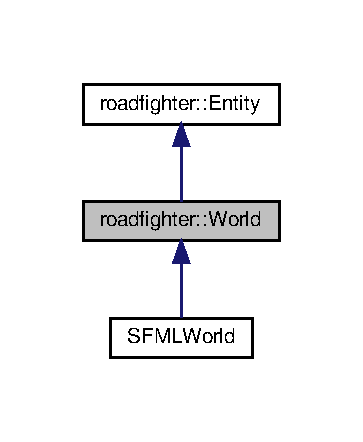
\includegraphics[width=174pt]{classroadfighter_1_1World__inherit__graph}
\end{center}
\end{figure}


Collaboration diagram for roadfighter\+:\+:World\+:\nopagebreak
\begin{figure}[H]
\begin{center}
\leavevmode
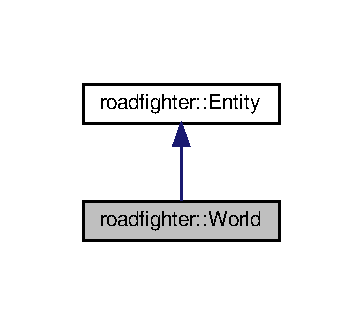
\includegraphics[width=174pt]{classroadfighter_1_1World__coll__graph}
\end{center}
\end{figure}
\subsection*{Public Member Functions}
\begin{DoxyCompactItemize}
\item 
\hyperlink{classroadfighter_1_1World_aa75df604422c5e2f160d082da86a50c4}{World} ()=default
\item 
\hyperlink{classroadfighter_1_1World_aa2f34c06cc3b81a6cd3f862137f1786b}{World} (const \hyperlink{classroadfighter_1_1World}{World} \&copy)=default
\item 
\hyperlink{classroadfighter_1_1World_aabd6663f3ee5533809152f154064cd89}{World} (\hyperlink{classroadfighter_1_1World}{World} \&\&move)=default
\item 
\mbox{\Hypertarget{classroadfighter_1_1World_ad1c38e0c158813af36113953003362d1}\label{classroadfighter_1_1World_ad1c38e0c158813af36113953003362d1}} 
{\bfseries World} (const std\+::shared\+\_\+ptr$<$ \hyperlink{classroadfighter_1_1EntityTransporter}{roadfighter\+::\+Entity\+Transporter} $>$ \&m\+\_\+\+Transporter)
\item 
\hyperlink{classroadfighter_1_1World}{World} \& \hyperlink{classroadfighter_1_1World_a31482bef8cfc86abc6326a4ffca74872}{operator=} (const \hyperlink{classroadfighter_1_1World}{World} \&other)=default
\item 
\hyperlink{classroadfighter_1_1World}{World} \& \hyperlink{classroadfighter_1_1World_ae2c0a8c3c8abd624087d5c5d82c2d5fd}{operator=} (\hyperlink{classroadfighter_1_1World}{World} \&\&other)=default
\item 
virtual \hyperlink{classroadfighter_1_1World_aea82fc8fead2cfb0032de65b1a198058}{$\sim$\+World} ()=default
\item 
void \hyperlink{classroadfighter_1_1World_abaf87df4c66473070ccf57bacbe56419}{set\+BackY} (double setback)
\item 
void \hyperlink{classroadfighter_1_1World_a880776b589376b1b4fd5ed4f26de4482}{update\+Movement} (double dt) override
\item 
void \hyperlink{classroadfighter_1_1World_a8d20efd557fc36fdf6218c0fdedd0b5a}{get\+New\+Entities} ()
\item 
void \hyperlink{classroadfighter_1_1World_ad04348a1285e8246abfacf32b600866f}{check\+Collision} ()
\item 
void \hyperlink{classroadfighter_1_1World_a90534263a154d6d7c1e8aef4e0138881}{draw} () override
\item 
void \hyperlink{classroadfighter_1_1World_a066592a75c8a38e241013707b429206c}{update\+Logic} () override
\item 
void \hyperlink{classroadfighter_1_1World_af7b77b0be8fee9e26093e2990f3889aa}{delete\+Unused} ()
\item 
double \hyperlink{classroadfighter_1_1World_a37fb93dcb90ec720a4ef17c43cf64dd4}{get\+Tick\+Movement} () const
\item 
\mbox{\Hypertarget{classroadfighter_1_1World_a82f62356ff13d7b52372f5568803686d}\label{classroadfighter_1_1World_a82f62356ff13d7b52372f5568803686d}} 
void {\bfseries dettach\+All\+Observers} ()
\end{DoxyCompactItemize}


\subsection{Constructor \& Destructor Documentation}
\mbox{\Hypertarget{classroadfighter_1_1World_aa75df604422c5e2f160d082da86a50c4}\label{classroadfighter_1_1World_aa75df604422c5e2f160d082da86a50c4}} 
\index{roadfighter\+::\+World@{roadfighter\+::\+World}!World@{World}}
\index{World@{World}!roadfighter\+::\+World@{roadfighter\+::\+World}}
\subsubsection{\texorpdfstring{World()}{World()}\hspace{0.1cm}{\footnotesize\ttfamily [1/3]}}
{\footnotesize\ttfamily roadfighter\+::\+World\+::\+World (\begin{DoxyParamCaption}{ }\end{DoxyParamCaption})\hspace{0.3cm}{\ttfamily [default]}}

default constructor for \hyperlink{classroadfighter_1_1World}{World} \mbox{\Hypertarget{classroadfighter_1_1World_aa2f34c06cc3b81a6cd3f862137f1786b}\label{classroadfighter_1_1World_aa2f34c06cc3b81a6cd3f862137f1786b}} 
\index{roadfighter\+::\+World@{roadfighter\+::\+World}!World@{World}}
\index{World@{World}!roadfighter\+::\+World@{roadfighter\+::\+World}}
\subsubsection{\texorpdfstring{World()}{World()}\hspace{0.1cm}{\footnotesize\ttfamily [2/3]}}
{\footnotesize\ttfamily roadfighter\+::\+World\+::\+World (\begin{DoxyParamCaption}\item[{const \hyperlink{classroadfighter_1_1World}{World} \&}]{copy }\end{DoxyParamCaption})\hspace{0.3cm}{\ttfamily [default]}}

copy constructor 
\begin{DoxyParams}{Parameters}
{\em copy} & the other world that is being copied \\
\hline
\end{DoxyParams}
\mbox{\Hypertarget{classroadfighter_1_1World_aabd6663f3ee5533809152f154064cd89}\label{classroadfighter_1_1World_aabd6663f3ee5533809152f154064cd89}} 
\index{roadfighter\+::\+World@{roadfighter\+::\+World}!World@{World}}
\index{World@{World}!roadfighter\+::\+World@{roadfighter\+::\+World}}
\subsubsection{\texorpdfstring{World()}{World()}\hspace{0.1cm}{\footnotesize\ttfamily [3/3]}}
{\footnotesize\ttfamily roadfighter\+::\+World\+::\+World (\begin{DoxyParamCaption}\item[{\hyperlink{classroadfighter_1_1World}{World} \&\&}]{move }\end{DoxyParamCaption})\hspace{0.3cm}{\ttfamily [default]}}

move constructor 
\begin{DoxyParams}{Parameters}
{\em Move} & the other world that is being moved in this one \\
\hline
\end{DoxyParams}
\mbox{\Hypertarget{classroadfighter_1_1World_aea82fc8fead2cfb0032de65b1a198058}\label{classroadfighter_1_1World_aea82fc8fead2cfb0032de65b1a198058}} 
\index{roadfighter\+::\+World@{roadfighter\+::\+World}!````~World@{$\sim$\+World}}
\index{````~World@{$\sim$\+World}!roadfighter\+::\+World@{roadfighter\+::\+World}}
\subsubsection{\texorpdfstring{$\sim$\+World()}{~World()}}
{\footnotesize\ttfamily virtual roadfighter\+::\+World\+::$\sim$\+World (\begin{DoxyParamCaption}{ }\end{DoxyParamCaption})\hspace{0.3cm}{\ttfamily [virtual]}, {\ttfamily [default]}}

destructor for \hyperlink{classroadfighter_1_1World}{World} 

\subsection{Member Function Documentation}
\mbox{\Hypertarget{classroadfighter_1_1World_ad04348a1285e8246abfacf32b600866f}\label{classroadfighter_1_1World_ad04348a1285e8246abfacf32b600866f}} 
\index{roadfighter\+::\+World@{roadfighter\+::\+World}!check\+Collision@{check\+Collision}}
\index{check\+Collision@{check\+Collision}!roadfighter\+::\+World@{roadfighter\+::\+World}}
\subsubsection{\texorpdfstring{check\+Collision()}{checkCollision()}}
{\footnotesize\ttfamily void roadfighter\+::\+World\+::check\+Collision (\begin{DoxyParamCaption}{ }\end{DoxyParamCaption})}

check the collision for all the entities and does the apropiate action \mbox{\Hypertarget{classroadfighter_1_1World_af7b77b0be8fee9e26093e2990f3889aa}\label{classroadfighter_1_1World_af7b77b0be8fee9e26093e2990f3889aa}} 
\index{roadfighter\+::\+World@{roadfighter\+::\+World}!delete\+Unused@{delete\+Unused}}
\index{delete\+Unused@{delete\+Unused}!roadfighter\+::\+World@{roadfighter\+::\+World}}
\subsubsection{\texorpdfstring{delete\+Unused()}{deleteUnused()}}
{\footnotesize\ttfamily void roadfighter\+::\+World\+::delete\+Unused (\begin{DoxyParamCaption}{ }\end{DoxyParamCaption})}

deletes all unused entities that are currently still in the entitie vectot \mbox{\Hypertarget{classroadfighter_1_1World_a90534263a154d6d7c1e8aef4e0138881}\label{classroadfighter_1_1World_a90534263a154d6d7c1e8aef4e0138881}} 
\index{roadfighter\+::\+World@{roadfighter\+::\+World}!draw@{draw}}
\index{draw@{draw}!roadfighter\+::\+World@{roadfighter\+::\+World}}
\subsubsection{\texorpdfstring{draw()}{draw()}}
{\footnotesize\ttfamily void roadfighter\+::\+World\+::draw (\begin{DoxyParamCaption}{ }\end{DoxyParamCaption})\hspace{0.3cm}{\ttfamily [override]}, {\ttfamily [virtual]}}

calls the draw function on all entities 

Implements \hyperlink{classroadfighter_1_1Entity_ac516f8005f969ad5a86c252e5a3640ee}{roadfighter\+::\+Entity}.



Reimplemented in \hyperlink{classSFMLWorld_aa0e1deda989ca494937054c5f5b139b0}{S\+F\+M\+L\+World}.

\mbox{\Hypertarget{classroadfighter_1_1World_a8d20efd557fc36fdf6218c0fdedd0b5a}\label{classroadfighter_1_1World_a8d20efd557fc36fdf6218c0fdedd0b5a}} 
\index{roadfighter\+::\+World@{roadfighter\+::\+World}!get\+New\+Entities@{get\+New\+Entities}}
\index{get\+New\+Entities@{get\+New\+Entities}!roadfighter\+::\+World@{roadfighter\+::\+World}}
\subsubsection{\texorpdfstring{get\+New\+Entities()}{getNewEntities()}}
{\footnotesize\ttfamily void roadfighter\+::\+World\+::get\+New\+Entities (\begin{DoxyParamCaption}{ }\end{DoxyParamCaption})}

takes all the entities that are currently in the transporter and puts them with the other entities \mbox{\Hypertarget{classroadfighter_1_1World_a37fb93dcb90ec720a4ef17c43cf64dd4}\label{classroadfighter_1_1World_a37fb93dcb90ec720a4ef17c43cf64dd4}} 
\index{roadfighter\+::\+World@{roadfighter\+::\+World}!get\+Tick\+Movement@{get\+Tick\+Movement}}
\index{get\+Tick\+Movement@{get\+Tick\+Movement}!roadfighter\+::\+World@{roadfighter\+::\+World}}
\subsubsection{\texorpdfstring{get\+Tick\+Movement()}{getTickMovement()}}
{\footnotesize\ttfamily double roadfighter\+::\+World\+::get\+Tick\+Movement (\begin{DoxyParamCaption}{ }\end{DoxyParamCaption}) const}

gets the amount of ticks that the world had to move loast movement\+Update \begin{DoxyReturn}{Returns}
a double 
\end{DoxyReturn}
\mbox{\Hypertarget{classroadfighter_1_1World_a31482bef8cfc86abc6326a4ffca74872}\label{classroadfighter_1_1World_a31482bef8cfc86abc6326a4ffca74872}} 
\index{roadfighter\+::\+World@{roadfighter\+::\+World}!operator=@{operator=}}
\index{operator=@{operator=}!roadfighter\+::\+World@{roadfighter\+::\+World}}
\subsubsection{\texorpdfstring{operator=()}{operator=()}\hspace{0.1cm}{\footnotesize\ttfamily [1/2]}}
{\footnotesize\ttfamily \hyperlink{classroadfighter_1_1World}{World}\& roadfighter\+::\+World\+::operator= (\begin{DoxyParamCaption}\item[{const \hyperlink{classroadfighter_1_1World}{World} \&}]{other }\end{DoxyParamCaption})\hspace{0.3cm}{\ttfamily [default]}}

copy assigment for \hyperlink{classroadfighter_1_1World}{World} 
\begin{DoxyParams}{Parameters}
{\em other} & the world that is being copied \\
\hline
\end{DoxyParams}
\begin{DoxyReturn}{Returns}
a new world that is equal to the other one 
\end{DoxyReturn}
\mbox{\Hypertarget{classroadfighter_1_1World_ae2c0a8c3c8abd624087d5c5d82c2d5fd}\label{classroadfighter_1_1World_ae2c0a8c3c8abd624087d5c5d82c2d5fd}} 
\index{roadfighter\+::\+World@{roadfighter\+::\+World}!operator=@{operator=}}
\index{operator=@{operator=}!roadfighter\+::\+World@{roadfighter\+::\+World}}
\subsubsection{\texorpdfstring{operator=()}{operator=()}\hspace{0.1cm}{\footnotesize\ttfamily [2/2]}}
{\footnotesize\ttfamily \hyperlink{classroadfighter_1_1World}{World}\& roadfighter\+::\+World\+::operator= (\begin{DoxyParamCaption}\item[{\hyperlink{classroadfighter_1_1World}{World} \&\&}]{other }\end{DoxyParamCaption})\hspace{0.3cm}{\ttfamily [default]}}

move assignment for world 
\begin{DoxyParams}{Parameters}
{\em other} & other world that is being moved \\
\hline
\end{DoxyParams}
\begin{DoxyReturn}{Returns}
a world that contains all the data of the first one 
\end{DoxyReturn}
\mbox{\Hypertarget{classroadfighter_1_1World_abaf87df4c66473070ccf57bacbe56419}\label{classroadfighter_1_1World_abaf87df4c66473070ccf57bacbe56419}} 
\index{roadfighter\+::\+World@{roadfighter\+::\+World}!set\+BackY@{set\+BackY}}
\index{set\+BackY@{set\+BackY}!roadfighter\+::\+World@{roadfighter\+::\+World}}
\subsubsection{\texorpdfstring{set\+Back\+Y()}{setBackY()}}
{\footnotesize\ttfamily void roadfighter\+::\+World\+::set\+BackY (\begin{DoxyParamCaption}\item[{double}]{setback }\end{DoxyParamCaption})}

this function subtracts the given paramater from all the y values of the m\+\_\+road\+Entities 
\begin{DoxyParams}{Parameters}
{\em setback} & the amount all entities should be setback \\
\hline
\end{DoxyParams}
\mbox{\Hypertarget{classroadfighter_1_1World_a066592a75c8a38e241013707b429206c}\label{classroadfighter_1_1World_a066592a75c8a38e241013707b429206c}} 
\index{roadfighter\+::\+World@{roadfighter\+::\+World}!update\+Logic@{update\+Logic}}
\index{update\+Logic@{update\+Logic}!roadfighter\+::\+World@{roadfighter\+::\+World}}
\subsubsection{\texorpdfstring{update\+Logic()}{updateLogic()}}
{\footnotesize\ttfamily void roadfighter\+::\+World\+::update\+Logic (\begin{DoxyParamCaption}{ }\end{DoxyParamCaption})\hspace{0.3cm}{\ttfamily [override]}, {\ttfamily [virtual]}}

updates the logic of this world and all the entities within 

Implements \hyperlink{classroadfighter_1_1Entity_a54c00f1af306290bae3e4b84e196566b}{roadfighter\+::\+Entity}.

\mbox{\Hypertarget{classroadfighter_1_1World_a880776b589376b1b4fd5ed4f26de4482}\label{classroadfighter_1_1World_a880776b589376b1b4fd5ed4f26de4482}} 
\index{roadfighter\+::\+World@{roadfighter\+::\+World}!update\+Movement@{update\+Movement}}
\index{update\+Movement@{update\+Movement}!roadfighter\+::\+World@{roadfighter\+::\+World}}
\subsubsection{\texorpdfstring{update\+Movement()}{updateMovement()}}
{\footnotesize\ttfamily void roadfighter\+::\+World\+::update\+Movement (\begin{DoxyParamCaption}\item[{double}]{dt }\end{DoxyParamCaption})\hspace{0.3cm}{\ttfamily [override]}, {\ttfamily [virtual]}}

this function updates the movement of all entities in this world by dt ticks 
\begin{DoxyParams}{Parameters}
{\em dt} & the amount of a tick the locations should be updated with \\
\hline
\end{DoxyParams}


Implements \hyperlink{classroadfighter_1_1Entity_a66614a11004d6f9516473f60b530f689}{roadfighter\+::\+Entity}.



The documentation for this class was generated from the following files\+:\begin{DoxyCompactItemize}
\item 
Game\+Logic/include/\+Entities/World.\+h\item 
Game\+Logic/\+Source/\+Entities/World.\+cpp\end{DoxyCompactItemize}

\chapter{File Documentation}
\hypertarget{Entity__Factory__base_8h}{}\section{Game\+Logic/include/\+Entity\+\_\+\+Factory\+\_\+base.h File Reference}
\label{Entity__Factory__base_8h}\index{Game\+Logic/include/\+Entity\+\_\+\+Factory\+\_\+base.\+h@{Game\+Logic/include/\+Entity\+\_\+\+Factory\+\_\+base.\+h}}
{\ttfamily \#include $<$memory$>$}\newline
{\ttfamily \#include \char`\"{}Entities/\+Entity.\+h\char`\"{}}\newline
{\ttfamily \#include \char`\"{}Observer/\+Score\+Observer.\+h\char`\"{}}\newline
{\ttfamily \#include \char`\"{}Input\+Controller.\+h\char`\"{}}\newline
{\ttfamily \#include \char`\"{}Entity\+Transporter.\+h\char`\"{}}\newline
{\ttfamily \#include \char`\"{}Observer/\+Observer\+Base.\+h\char`\"{}}\newline
Include dependency graph for Entity\+\_\+\+Factory\+\_\+base.\+h\+:
\nopagebreak
\begin{figure}[H]
\begin{center}
\leavevmode
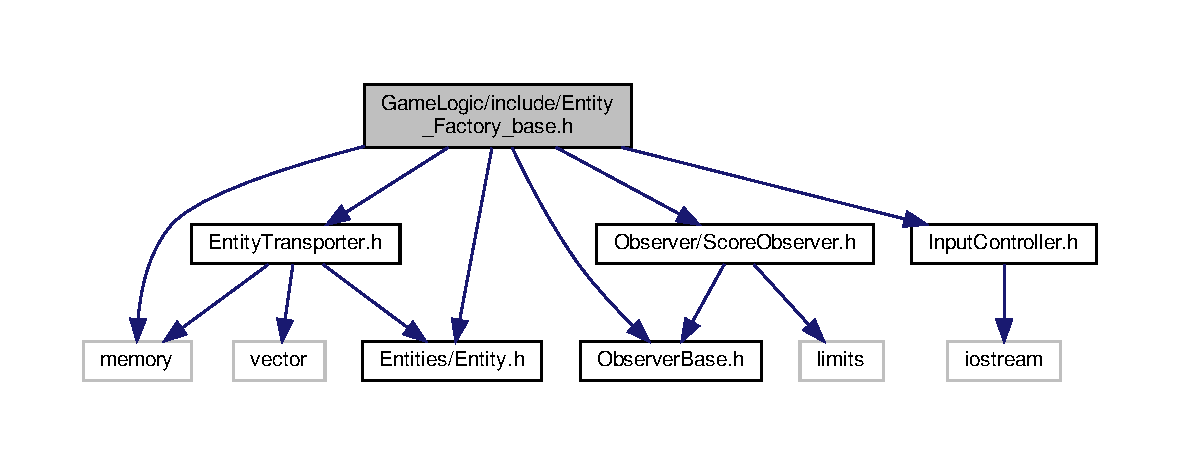
\includegraphics[width=350pt]{Entity__Factory__base_8h__incl}
\end{center}
\end{figure}
This graph shows which files directly or indirectly include this file\+:
\nopagebreak
\begin{figure}[H]
\begin{center}
\leavevmode
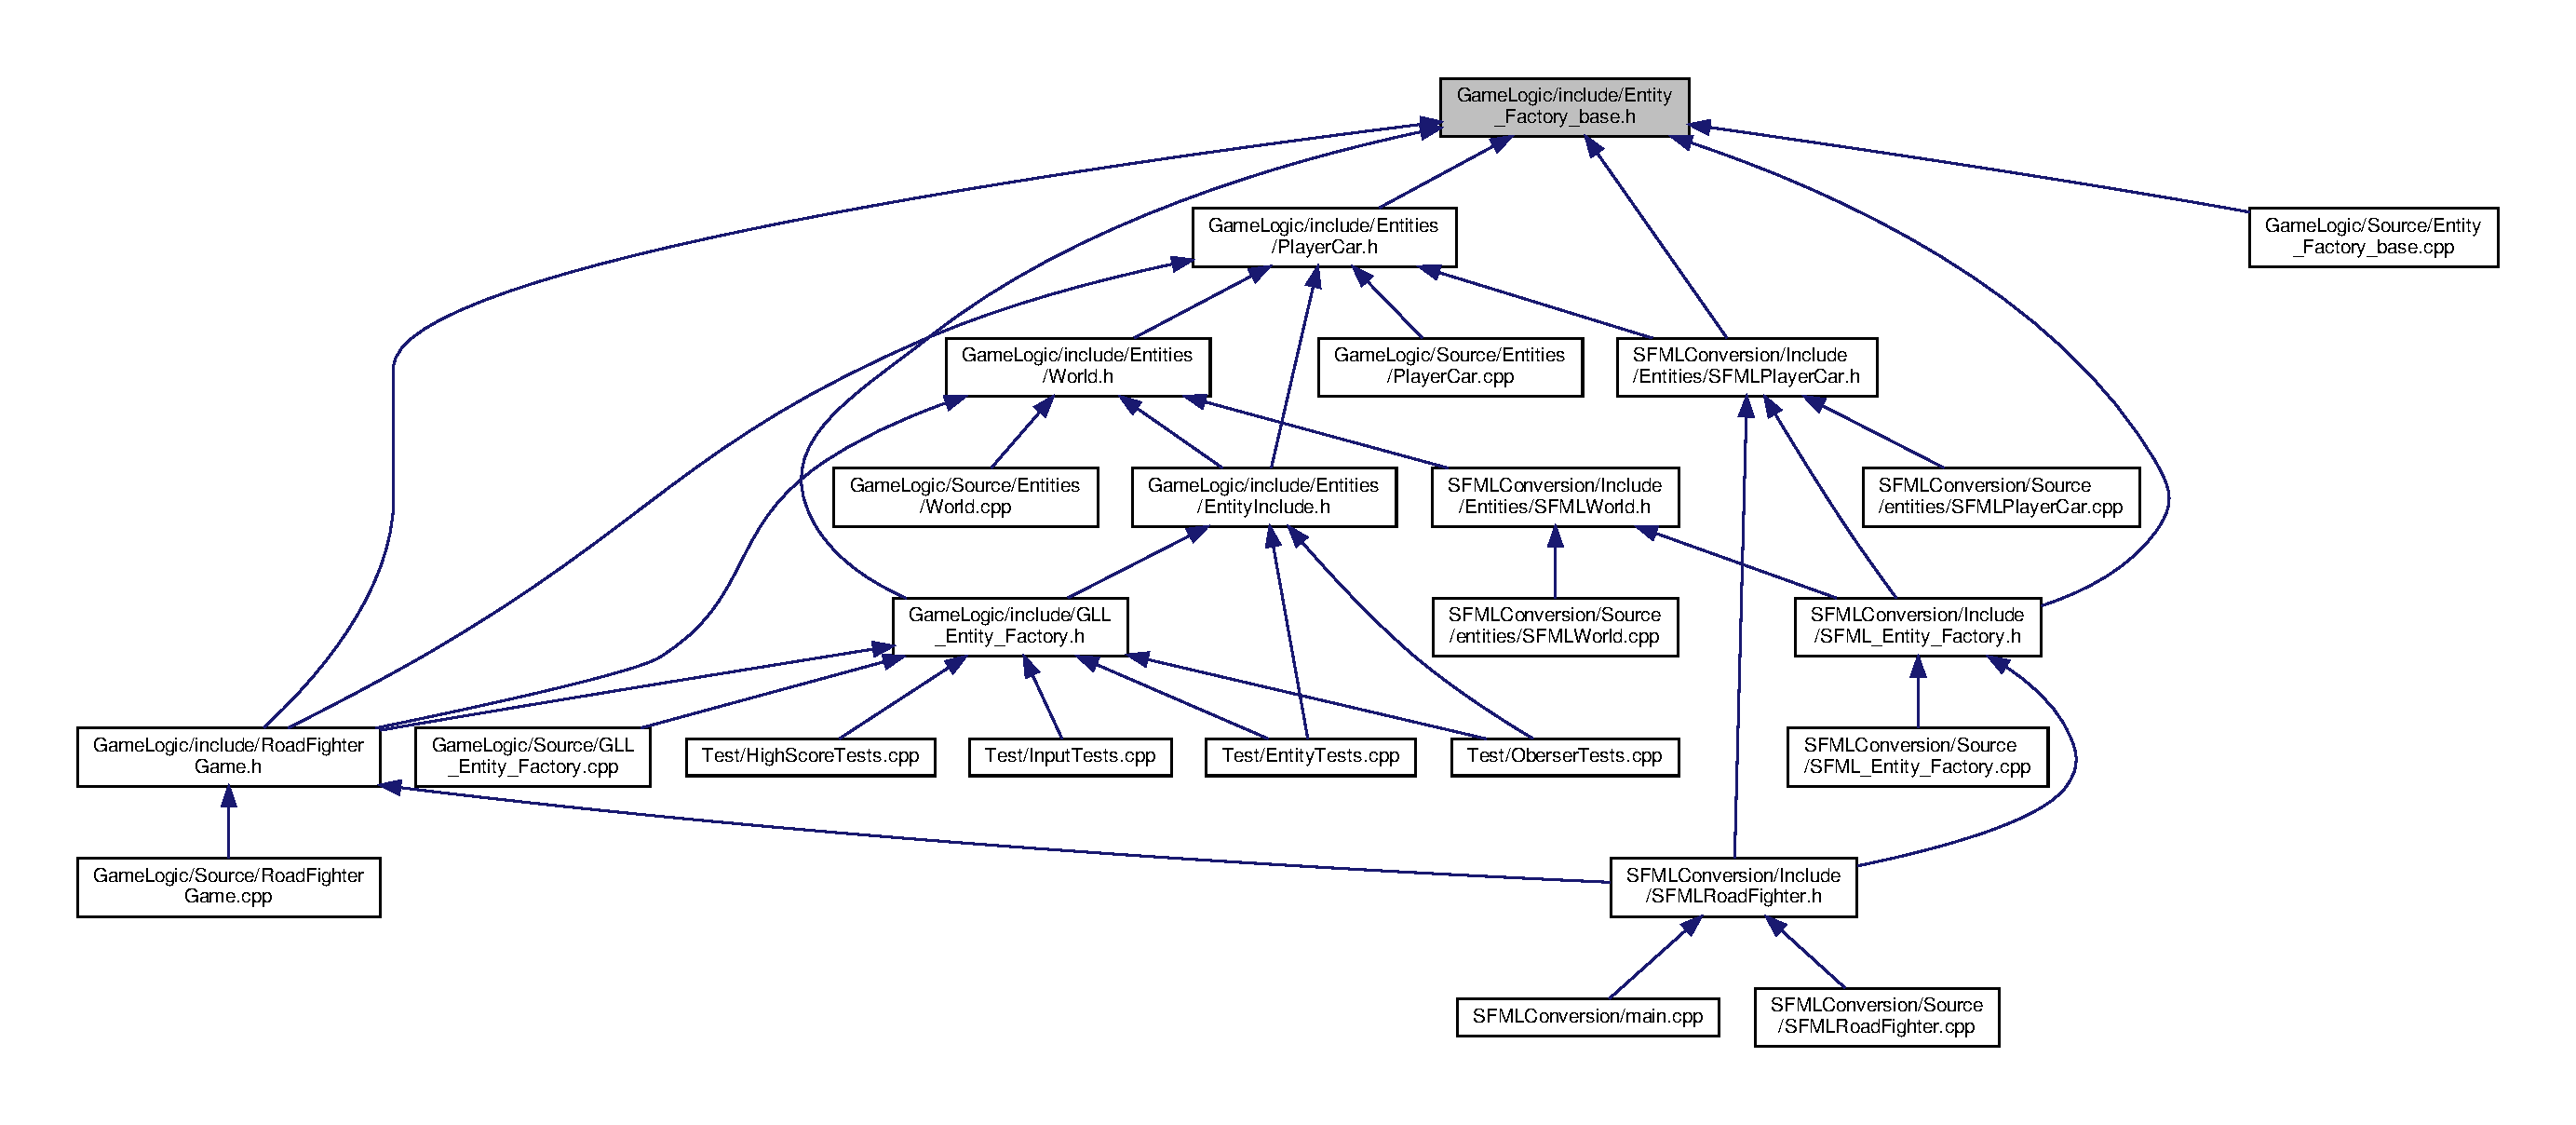
\includegraphics[width=350pt]{Entity__Factory__base_8h__dep__incl}
\end{center}
\end{figure}
\subsection*{Classes}
\begin{DoxyCompactItemize}
\item 
class \hyperlink{classroadfighter_1_1Entity__Factory__base}{roadfighter\+::\+Entity\+\_\+\+Factory\+\_\+base}
\end{DoxyCompactItemize}
\subsection*{Namespaces}
\begin{DoxyCompactItemize}
\item 
 \hyperlink{namespaceroadfighter}{roadfighter}
\end{DoxyCompactItemize}


\subsection{Detailed Description}
a abstract class that should be overidden and is used to represent the abstract factory that is used to create all the entities \begin{DoxyAuthor}{Author}
Thibaut Van Goethem 
\end{DoxyAuthor}

\hypertarget{EntityTransporter_8h}{}\section{Game\+Logic/include/\+Entity\+Transporter.h File Reference}
\label{EntityTransporter_8h}\index{Game\+Logic/include/\+Entity\+Transporter.\+h@{Game\+Logic/include/\+Entity\+Transporter.\+h}}
{\ttfamily \#include \char`\"{}Entities/\+Entity.\+h\char`\"{}}\newline
{\ttfamily \#include $<$memory$>$}\newline
{\ttfamily \#include $<$vector$>$}\newline
Include dependency graph for Entity\+Transporter.\+h\+:\nopagebreak
\begin{figure}[H]
\begin{center}
\leavevmode
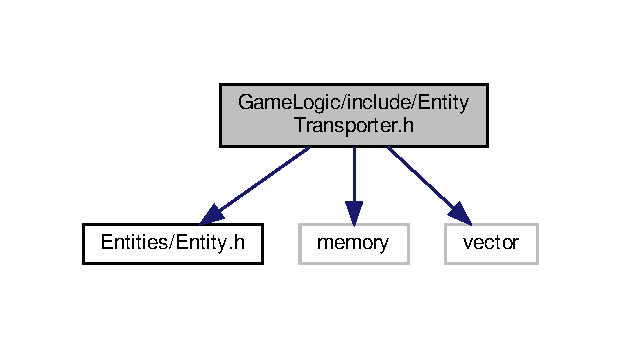
\includegraphics[width=298pt]{EntityTransporter_8h__incl}
\end{center}
\end{figure}
This graph shows which files directly or indirectly include this file\+:\nopagebreak
\begin{figure}[H]
\begin{center}
\leavevmode
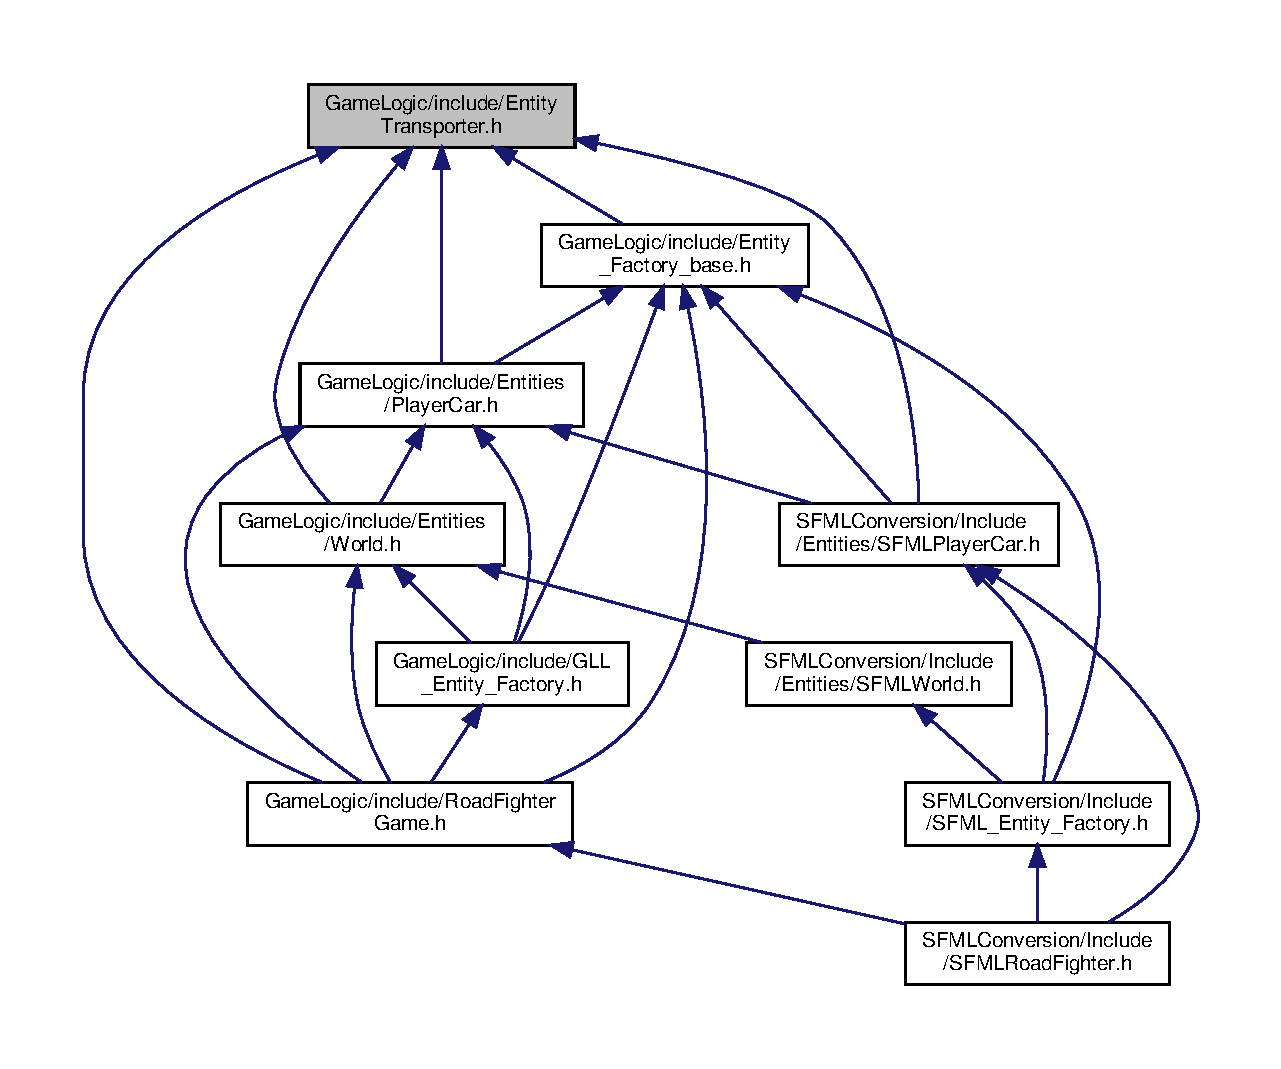
\includegraphics[width=350pt]{EntityTransporter_8h__dep__incl}
\end{center}
\end{figure}
\subsection*{Classes}
\begin{DoxyCompactItemize}
\item 
class \hyperlink{classroadfighter_1_1EntityTransporter}{roadfighter\+::\+Entity\+Transporter}
\end{DoxyCompactItemize}


\subsection{Detailed Description}
this file is for the entity\+Transporter that will regulate the exchange of entities between the game and the world 
\hypertarget{GLL__Entity__Factory_8h}{}\section{Game\+Logic/include/\+G\+L\+L\+\_\+\+Entity\+\_\+\+Factory.h File Reference}
\label{GLL__Entity__Factory_8h}\index{Game\+Logic/include/\+G\+L\+L\+\_\+\+Entity\+\_\+\+Factory.\+h@{Game\+Logic/include/\+G\+L\+L\+\_\+\+Entity\+\_\+\+Factory.\+h}}
{\ttfamily \#include $<$memory$>$}\newline
{\ttfamily \#include \char`\"{}Entity\+\_\+\+Factory\+\_\+base.\+h\char`\"{}}\newline
{\ttfamily \#include \char`\"{}Entities/\+Bullet.\+h\char`\"{}}\newline
{\ttfamily \#include \char`\"{}Entities/\+Player\+Car.\+h\char`\"{}}\newline
{\ttfamily \#include \char`\"{}Entities/\+Racing\+Car.\+h\char`\"{}}\newline
{\ttfamily \#include \char`\"{}Entities/\+World.\+h\char`\"{}}\newline
Include dependency graph for G\+L\+L\+\_\+\+Entity\+\_\+\+Factory.\+h\+:\nopagebreak
\begin{figure}[H]
\begin{center}
\leavevmode
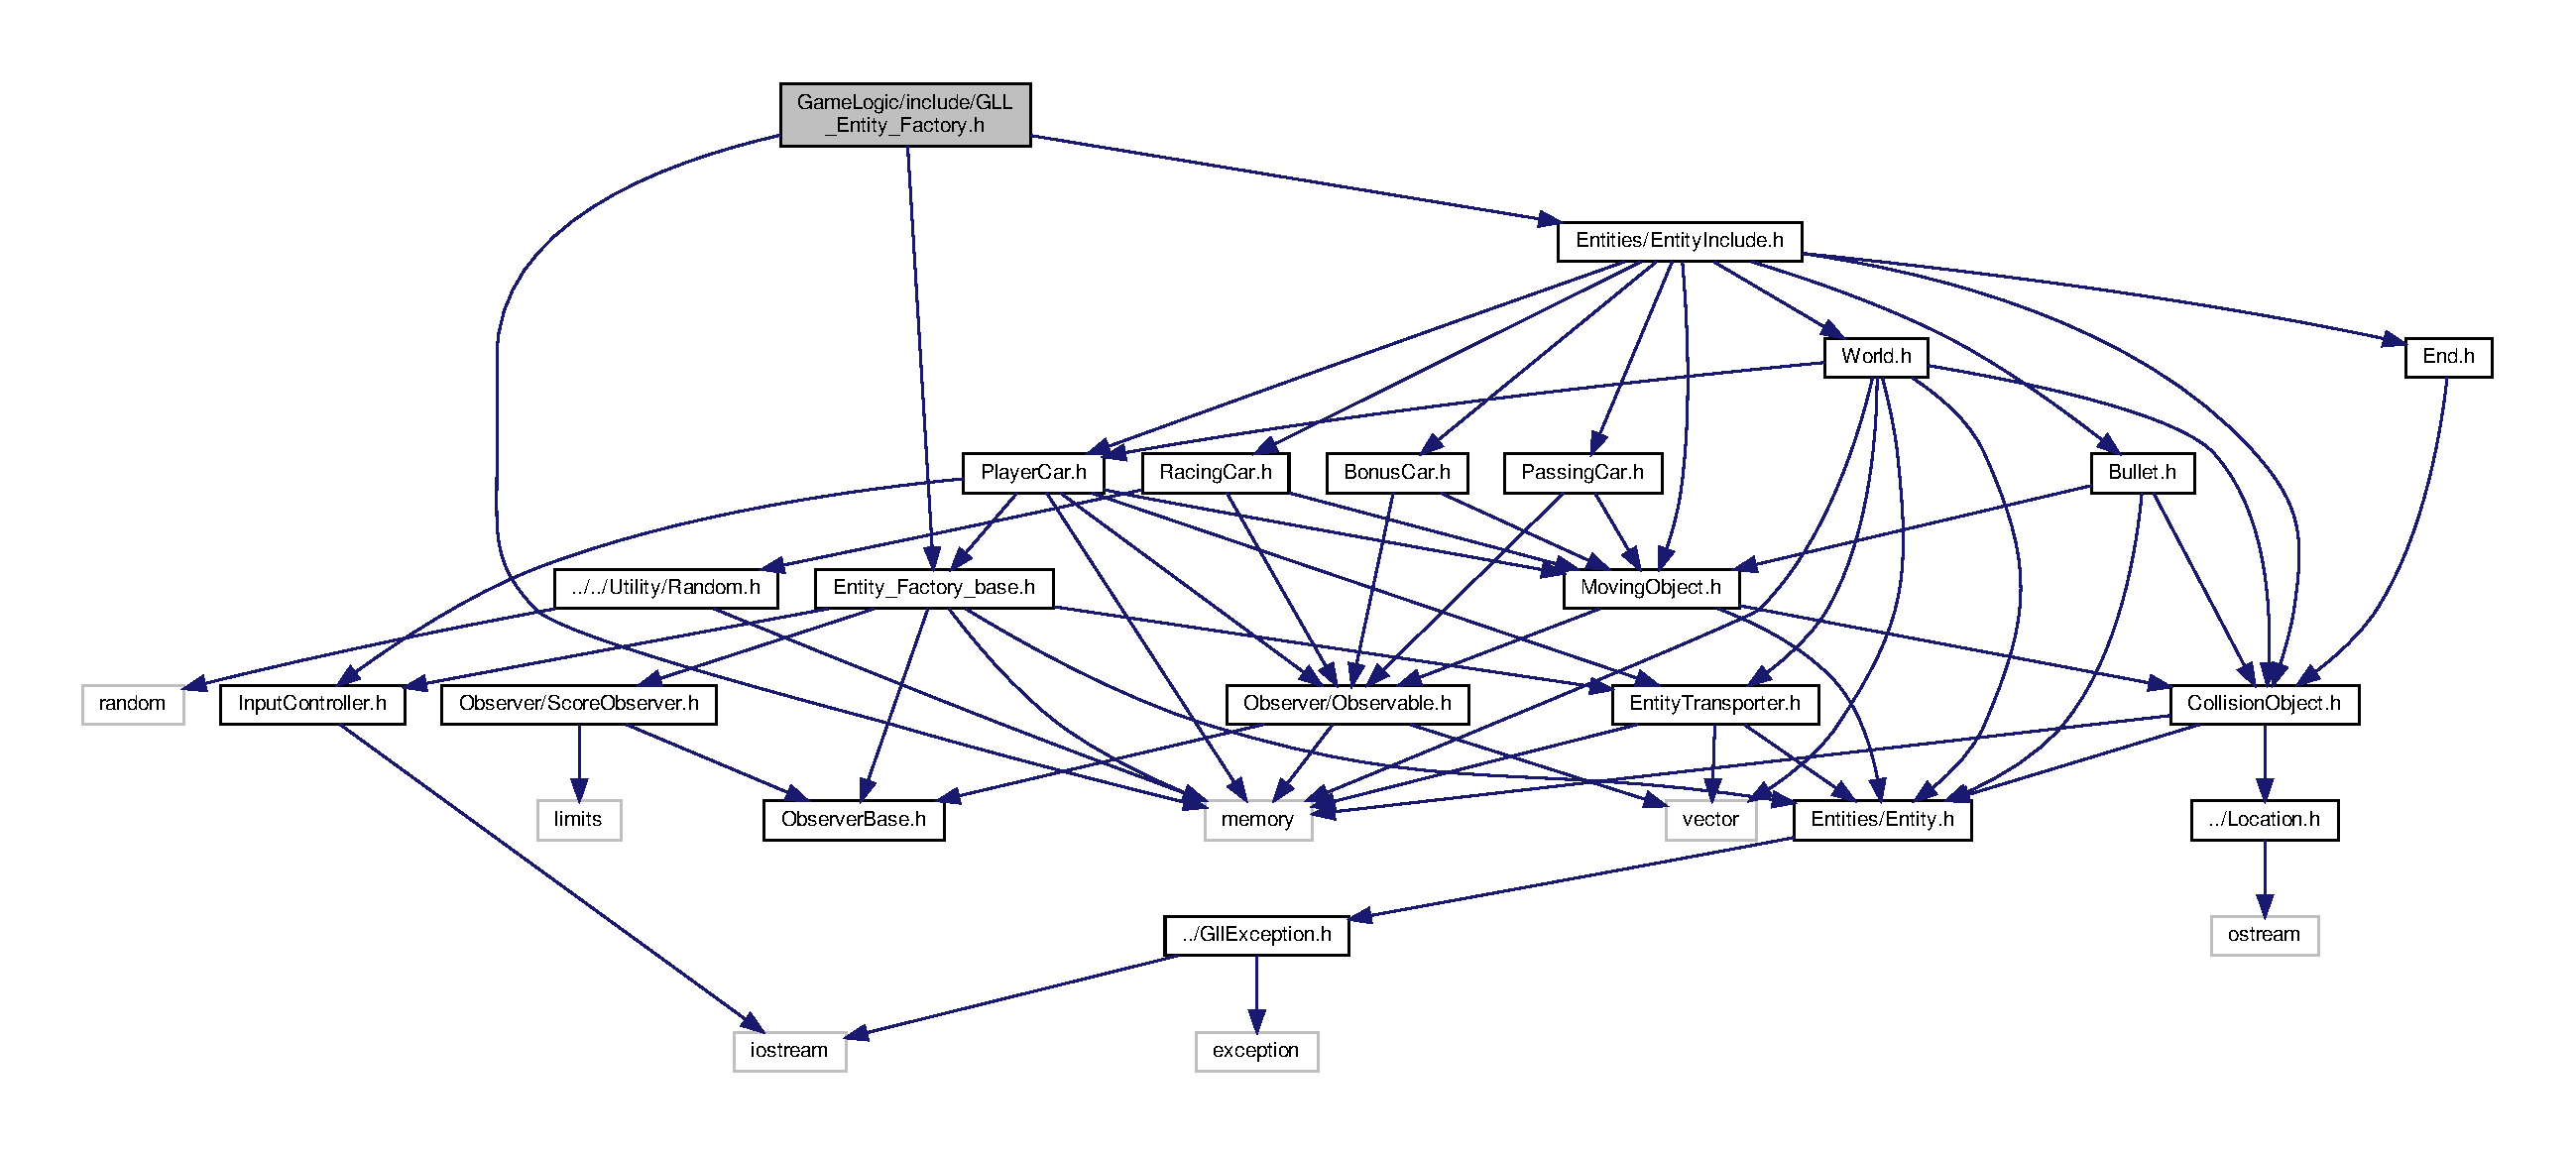
\includegraphics[width=350pt]{GLL__Entity__Factory_8h__incl}
\end{center}
\end{figure}
This graph shows which files directly or indirectly include this file\+:\nopagebreak
\begin{figure}[H]
\begin{center}
\leavevmode
\includegraphics[width=236pt]{GLL__Entity__Factory_8h__dep__incl}
\end{center}
\end{figure}
\subsection*{Classes}
\begin{DoxyCompactItemize}
\item 
class \hyperlink{classroadfighter_1_1GLL__Entity__Factory}{roadfighter\+::\+G\+L\+L\+\_\+\+Entity\+\_\+\+Factory}
\end{DoxyCompactItemize}


\subsection{Detailed Description}
this file contains a class derived from teh base antitie factory and will be teh default value if no abstract factory is given to the roadfighter game this factory will be used to create all sorts of entities 
\hypertarget{InputController_8h}{}\section{Game\+Logic/include/\+Input\+Controller.h File Reference}
\label{InputController_8h}\index{Game\+Logic/include/\+Input\+Controller.\+h@{Game\+Logic/include/\+Input\+Controller.\+h}}
{\ttfamily \#include $<$iostream$>$}\newline
Include dependency graph for Input\+Controller.\+h\+:\nopagebreak
\begin{figure}[H]
\begin{center}
\leavevmode
\includegraphics[width=255pt]{InputController_8h__incl}
\end{center}
\end{figure}
This graph shows which files directly or indirectly include this file\+:\nopagebreak
\begin{figure}[H]
\begin{center}
\leavevmode
\includegraphics[width=350pt]{InputController_8h__dep__incl}
\end{center}
\end{figure}
\subsection*{Classes}
\begin{DoxyCompactItemize}
\item 
class \hyperlink{classroadfighter_1_1InputController}{roadfighter\+::\+Input\+Controller}
\end{DoxyCompactItemize}
\subsection*{Enumerations}
\begin{DoxyCompactItemize}
\item 
\mbox{\Hypertarget{InputController_8h_a7d7f8a685d9171fc4243ae6011fc342a}\label{InputController_8h_a7d7f8a685d9171fc4243ae6011fc342a}} 
enum {\bfseries E\+Vert\+Move} \{ {\bfseries v\+\_\+none}, 
{\bfseries v\+\_\+accel}, 
{\bfseries v\+\_\+decel}
 \}
\item 
\mbox{\Hypertarget{InputController_8h_a4f147cd0e746b046e0ce2fc14fa4e180}\label{InputController_8h_a4f147cd0e746b046e0ce2fc14fa4e180}} 
enum {\bfseries E\+Hor\+Move} \{ {\bfseries h\+\_\+none}, 
{\bfseries h\+\_\+left}, 
{\bfseries h\+\_\+right}
 \}
\end{DoxyCompactItemize}


\subsection{Detailed Description}
this file contains the movecontroller class that handles the acces of current keyboard input over the whole roadfighter game it also contains 2 enums used to represent vertical and horizontal movement 
\hypertarget{Location_8h}{}\section{Game\+Logic/include/\+Location.h File Reference}
\label{Location_8h}\index{Game\+Logic/include/\+Location.\+h@{Game\+Logic/include/\+Location.\+h}}
{\ttfamily \#include $<$ostream$>$}\newline
Include dependency graph for Location.\+h\+:\nopagebreak
\begin{figure}[H]
\begin{center}
\leavevmode
\includegraphics[width=228pt]{Location_8h__incl}
\end{center}
\end{figure}
This graph shows which files directly or indirectly include this file\+:\nopagebreak
\begin{figure}[H]
\begin{center}
\leavevmode
\includegraphics[width=350pt]{Location_8h__dep__incl}
\end{center}
\end{figure}
\subsection*{Classes}
\begin{DoxyCompactItemize}
\item 
class \hyperlink{classroadfighter_1_1Location}{roadfighter\+::\+Location}
\end{DoxyCompactItemize}


\subsection{Detailed Description}
this file has a very simple 2d location class that is used in every collision object to represetn it\textquotesingle{}s position 
\hypertarget{RoadFighterGame_8h}{}\section{Game\+Logic/include/\+Road\+Fighter\+Game.h File Reference}
\label{RoadFighterGame_8h}\index{Game\+Logic/include/\+Road\+Fighter\+Game.\+h@{Game\+Logic/include/\+Road\+Fighter\+Game.\+h}}
{\ttfamily \#include $<$memory$>$}\newline
{\ttfamily \#include \char`\"{}Entity\+\_\+\+Factory\+\_\+base.\+h\char`\"{}}\newline
{\ttfamily \#include \char`\"{}Entities/\+World.\+h\char`\"{}}\newline
{\ttfamily \#include \char`\"{}Entities/\+Player\+Car.\+h\char`\"{}}\newline
{\ttfamily \#include \char`\"{}G\+L\+L\+\_\+\+Entity\+\_\+\+Factory.\+h\char`\"{}}\newline
{\ttfamily \#include \char`\"{}Entities/\+Entity.\+h\char`\"{}}\newline
{\ttfamily \#include \char`\"{}Input\+Controller.\+h\char`\"{}}\newline
{\ttfamily \#include \char`\"{}Entity\+Transporter.\+h\char`\"{}}\newline
{\ttfamily \#include \char`\"{}../\+Utility/\+Random.\+h\char`\"{}}\newline
{\ttfamily \#include \char`\"{}Observer/\+Score\+Observer.\+h\char`\"{}}\newline
{\ttfamily \#include \char`\"{}High\+Score\+Manager.\+h\char`\"{}}\newline
Include dependency graph for Road\+Fighter\+Game.\+h\+:\nopagebreak
\begin{figure}[H]
\begin{center}
\leavevmode
\includegraphics[width=350pt]{RoadFighterGame_8h__incl}
\end{center}
\end{figure}
This graph shows which files directly or indirectly include this file\+:\nopagebreak
\begin{figure}[H]
\begin{center}
\leavevmode
\includegraphics[width=236pt]{RoadFighterGame_8h__dep__incl}
\end{center}
\end{figure}
\subsection*{Classes}
\begin{DoxyCompactItemize}
\item 
class \hyperlink{classroadfighter_1_1RoadFighterGame}{roadfighter\+::\+Road\+Fighter\+Game}
\end{DoxyCompactItemize}
\subsection*{Enumerations}
\begin{DoxyCompactItemize}
\item 
\mbox{\Hypertarget{RoadFighterGame_8h_ad5f7291dfb2d888ac0c59e10f59ba8a0}\label{RoadFighterGame_8h_ad5f7291dfb2d888ac0c59e10f59ba8a0}} 
enum {\bfseries E\+Game\+Status} \{ {\bfseries game\+Running}, 
{\bfseries game\+Ending}, 
{\bfseries game\+Ended}, 
{\bfseries game\+Paused}
 \}
\end{DoxyCompactItemize}


\subsection{Detailed Description}
this file contains a class that will be the brains of the logic behind the roadfighter game 
%--- End generated contents ---

% Index
\backmatter
\newpage
\phantomsection
\clearemptydoublepage
\addcontentsline{toc}{chapter}{Index}
\printindex

\end{document}
